%%%%%%%%%%%%%%%%%%%%%%%%%%%%%%%%%%%%%%%%%%%%%%%%%%%%%%%%%%%%%%%%%%%%%%
% Oslo CTM3
% User manual
%%%%%%%%%%%%%%%%%%%%%%%%%%%%%%%%%%%%%%%%%%%%%%%%%%%%%%%%%%%%%%%%%%%%%%
%
% CHECK TAGS TOBEUPDATED
%
%%%%%%%%%%%%%%%%%%%%%%%%%%%%%%%%%%%%%%%%%%%%%%%%%%%%%%%%%%%%%%%%%%%%%%
%
% This manual has been written over several years, mainly 2008-2015,
% with updates during 2016-2017.
%
% Amund Sovde Haslerud, 2018
%   meteorologen@gmail.com
%%%%%%%%%%%%%%%%%%%%%%%%%%%%%%%%%%%%%%%%%%%%%%%%%%%%%%%%%%%%%%%%%%%%%%
% Compiling:
%  Use latex, bibtex and makeindex. See batch file compile_manual.
%  Some of the eps-figures (produced using python3 on linux) do not
%  work well with windows Latex (MixTex).
%%%%%%%%%%%%%%%%%%%%%%%%%%%%%%%%%%%%%%%%%%%%%%%%%%%%%%%%%%%%%%%%%%%%%%
% Search keywords to easily locate sections
%   Abstract:                 #ABS
%   Table of contents:        #TOC
%   Introduction:             #INTRO
%   Get started:              #GETS
%   Intro to source code:     #SRC
%   Program structure:        #PROG
%   Programming guidelines:   #GUIDE
%   Transport:                #TRSP
%   Wet and dry deposition:   #SCAV
%   Emissions:                #EMISSION
%   QSSA chemical integrator: #QSSA
%   Tropospheric chemistry:   #TROPC
%   Stratospheric chemistry:  #STRATC
%   Photochemistry:           #PHOT
%   Sulphate:                 #SULF
%   Black and organic carbon: #BCOC
%   Mineral dust:             #DUST
%   Seasalt:                  #SALT
%   Nitrate:                  #NIT
%   M7:                       #M7
%   Physics:                  #PHY
%   Diagnostics:              #DIAG
%
%   Appendix:                 #APPX
%   Description model files:  #MODFILES
%   SVN/Subversion:           #SVN
%   Technical notes:          #TECH
%   Things to revise:         #REVISETHIS
%   Compiler options:         #COMP
%   HPC:                      #HPC
%   Libraries:                #XLIB
%   Meteorological data:      #METDATA
%   Trouble shooting:         #TROUBLE
%   Peer-reviewed papers:     #PEER
%   Contact information:      #CONTACT
%   Acknowledgements:         #ACKN
%%%%%%%%%%%%%%%%%%%%%%%%%%%%%%%%%%%%%%%%%%%%%%%%%%%%%%%%%%%%%%%%%%%%%%
% Set up the document page and style
%%%%%%%%%%%%%%%%%%%%%%%%%%%%%%%%%%%%%%%%%%%%%%%%%%%%%%%%%%%%%%%%%%%%%%
\documentclass[a4paper,10pt,twocolumn]{article}
\usepackage[latin1]{inputenc}
\usepackage[T1]{fontenc}
\usepackage[usenames]{color}
\usepackage{graphicx}
% To make eps work in pdflatex
\usepackage{epstopdf}
\usepackage{fancyhdr}
% For references layout
\usepackage{natbib}
% To make index at the end
\usepackage{makeidx}
\makeindex
\usepackage{multicol}

\usepackage[singlelinecheck=false]{caption}

% side margin and text width
\addtolength{\oddsidemargin}{-2.5mm}
\addtolength{\evensidemargin}{-2.5mm}
\addtolength{\textwidth}{5mm}

% vertical dimension
\addtolength{\topmargin}{-27mm}
\addtolength{\textheight}{50mm} %{68pt}

% text width
%\oddsidemargin 0mm
%\evensidemargin 0mm
%\textwidth 160mm

\makeatletter
\setlength{\@fptop}{0pt}
\makeatother

% indent
\setlength{\parindent}{0mm}
% How many levels of subdirectories should be allowed
\setcounter{secnumdepth}{5}
%%%%%%%%%%%%%%%%%%%%%%%%%%%%%%%%%%%%%%%%%%%%%%%%%%%%%%%%%%%%%%%%%%%%%%

%%%%%%%%%%%%%%%%%%%%%%%%%%%%%%%%%%%%%%%%%%%%%%%%%%%%%%%%%%%%%%%%%%%%%%
% Setting up some short commands
% Line commands
\newcommand{\HRule}{\rule{\linewidth}{1mm}}
\newcommand{\VRule}{\rule{1mm}{60mm}}
\newcommand{\strek}{\rule[2mm]{\linewidth}{0.1mm}\vspace*{-1.5mm}}
\newcommand{\TynnRule}{\rule{\linewidth}{0.5mm}}
\newcommand{\MidtStrek}{\rule[0.8mm]{6mm}{0.1mm}}
% Bullet command
\newcommand{\bul}{$\bullet$\ }
% Tab command
\newcommand{\atab}{\hspace*{5mm}}

% Commands for names/text
\newcommand{\model}{Oslo~CTM3}
\newcommand{\version}{v1.0}
\newcommand{\oldmodel}{Oslo~CTM2}
\newcommand{\pmain}{\mbox{pmain}}
\newcommand{\ucimodel}{UCI CTM}
\newcommand{\qcodelastupdate}{6.1b}
\newcommand{\osloctmmail}{\texttt{oslo-ctm@geo.uio.no}}
\newcommand{\osloctmweb}{\texttt{not~available}}
% Commands for e.g. files and directories
\newcommand{\pmainf}{\mbox{\it pmain.f90}}
\newcommand{\makefile}{{\it Makefile}}
\newcommand{\ratjfile}{{\it ratj\_oc.d}}
\newcommand{\tracerlist}{{\it tracer\_list.d}}
\newcommand{\wetscavlist}{{\it scavenging\_wet.dat}}
\newcommand{\dryscavlist}{{\it scavenging\_dry.dat}}
\newcommand{\dryscavlistOC}{{\it drydep.ctm}}
\newcommand{\fjxscatfile}{{\it FJX\_scat.dat}}
\newcommand{\fjxumaerfile}{{\it FJX\_UMaer.dat}}
\newcommand{\maininput}{{\it LxxCTM.inp}}
\newcommand{\diaginput}{{\it LxxCTM.inp}}
\newcommand{\emisfile}{{\it Ltracer\_emis\_xxxx.inp}}
\newcommand{\oslopath}{{\it OSLO}}
\newcommand{\emislistdir}{{\it tables}}
% Abel paths
\newcommand{\emispath}{{\it /work/projects/cicero/ctm\_input/EMIS}}
\newcommand{\dustpath}{\oslopath/{\it DEAD\_COLUMN}}
\newcommand{\hpcdatageo}{{\it /work/projects/cicero/ctm\_input}}
\newcommand{\inputctmiii}{{\it Input\_CTM3}}
% Geo/Cicero paths
\newcommand{\ctmciceropath}{{\it /div/amoc/d4-4/oslo-ctm/}}
\newcommand{\ctmgeopath}{{\it /div/amoc/d4-4/oslo-ctm/archive\_ctm/}}
\newcommand{\toolspath}{{\it ctm\_tools/}}
\newcommand{\inputpath}{{\it input\_files/}}
\newcommand{\boxpath}{{\it box\_models/}}
\newcommand{\metdatastore}{{\it /div/pdo/metdata/}}
% Other paths
\newcommand{\generateOpenIFS}{{\it generateOpenIFS}}


% New environments
\newenvironment{itemize2} {
\begin{itemize}\addtolength{\itemsep}{-0.3\baselineskip}\vspace*{-0.95\baselineskip}
}{\end{itemize} }
\newenvironment{description2} {
\begin{description}\addtolength{\itemsep}{-0.6\baselineskip}
}{\end{description} }
%%%%%%%%%%%%%%%%%%%%%%%%%%%%%%%%%%%%%%%%%%%%%%%%%%%%%%%%%%%%%%%%%%%%%%
%%%%%%%%%%%%%%%%%%%%%%%%%%%%%%%%%%%%%%%%%%%%%%%%%%%%%%%%%%%%%%%%%%%%%%
%%%%%%%%%%%%%%%%%%%%%%%%%%%%%%%%%%%%%%%%%%%%%%%%%%%%%%%%%%%%%%%%%%%%%%
% Begin document
%%%%%%%%%%%%%%%%%%%%%%%%%%%%%%%%%%%%%%%%%%%%%%%%%%%%%%%%%%%%%%%%%%%%%%
%%%%%%%%%%%%%%%%%%%%%%%%%%%%%%%%%%%%%%%%%%%%%%%%%%%%%%%%%%%%%%%%%%%%%%
%%%%%%%%%%%%%%%%%%%%%%%%%%%%%%%%%%%%%%%%%%%%%%%%%%%%%%%%%%%%%%%%%%%%%%
\begin{document}
%%%%%%%%%%%%%%%%%%%%%%%%%%%%%%%%%%%%%%%%%%%%%%%%%%%%%%%%%%%%%%%%%%%%%%




%%%%%%%%%%%%%%%%%%%%%%%%%%%%%%%%%%%%%%%%%%%%%%%%%%%%%%%%%%%%%%%%%%%%%%
% Title
%%%%%%%%%%%%%%%%%%%%%%%%%%%%%%%%%%%%%%%%%%%%%%%%%%%%%%%%%%%%%%%%%%%%%%
\pagestyle{empty}
\twocolumn[\flushright
{\bf \huge \model}\\
\vspace*{3mm}
{\bf \Large \version}\\
\vspace*{3mm}
{\bf \Large User manual}\\
\vspace*{6mm}
\TynnRule\\
\vspace*{3mm}
\flushleft
{\bf \large Amund S{\o}vde Haslerud}\\
{\bf CICERO Center for International Climate Research}\\
\vspace*{3mm}
{\bf \today}\\
\vspace*{3mm}
\TynnRule\\
\vspace*{5mm}
\bigskip

\begin{picture}(500,500)
\put (0,220){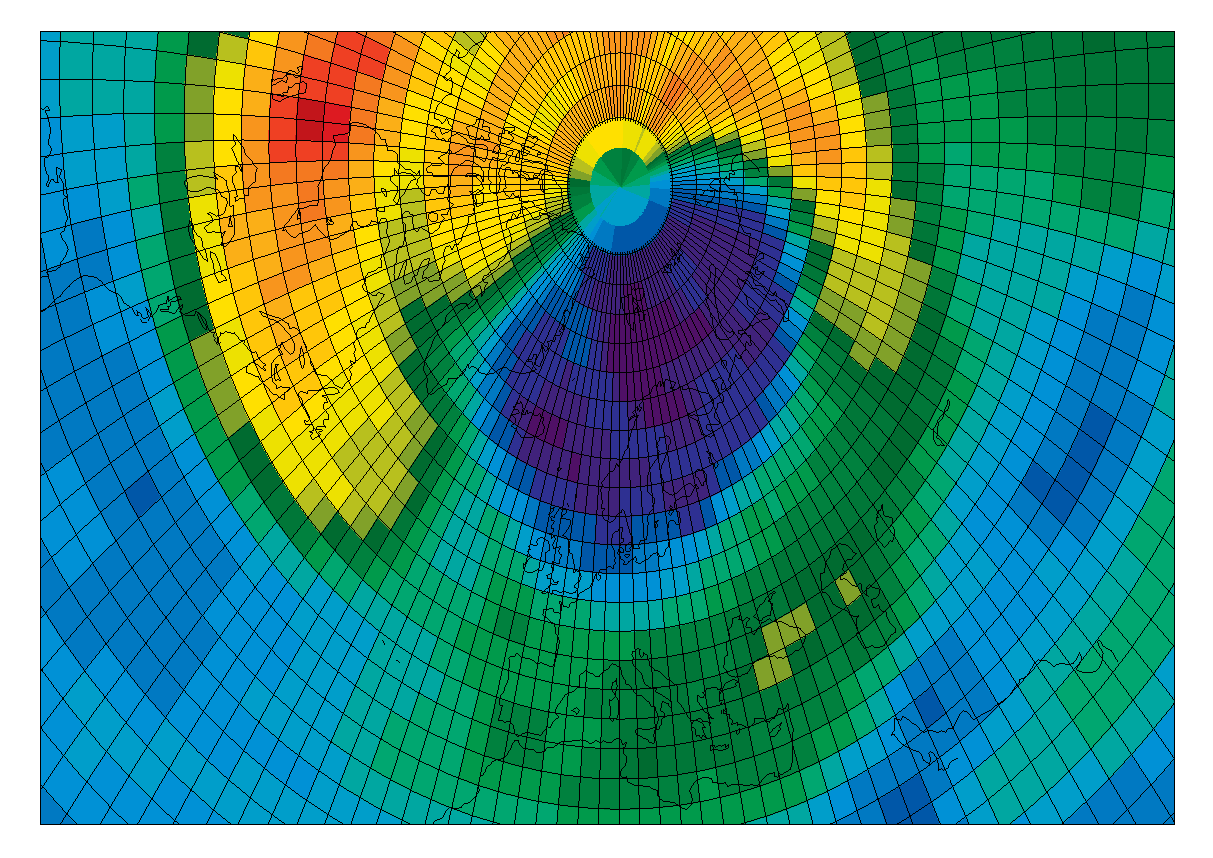
\includegraphics[width=250pt]{figures/c3manfront1}}
\put (150,0){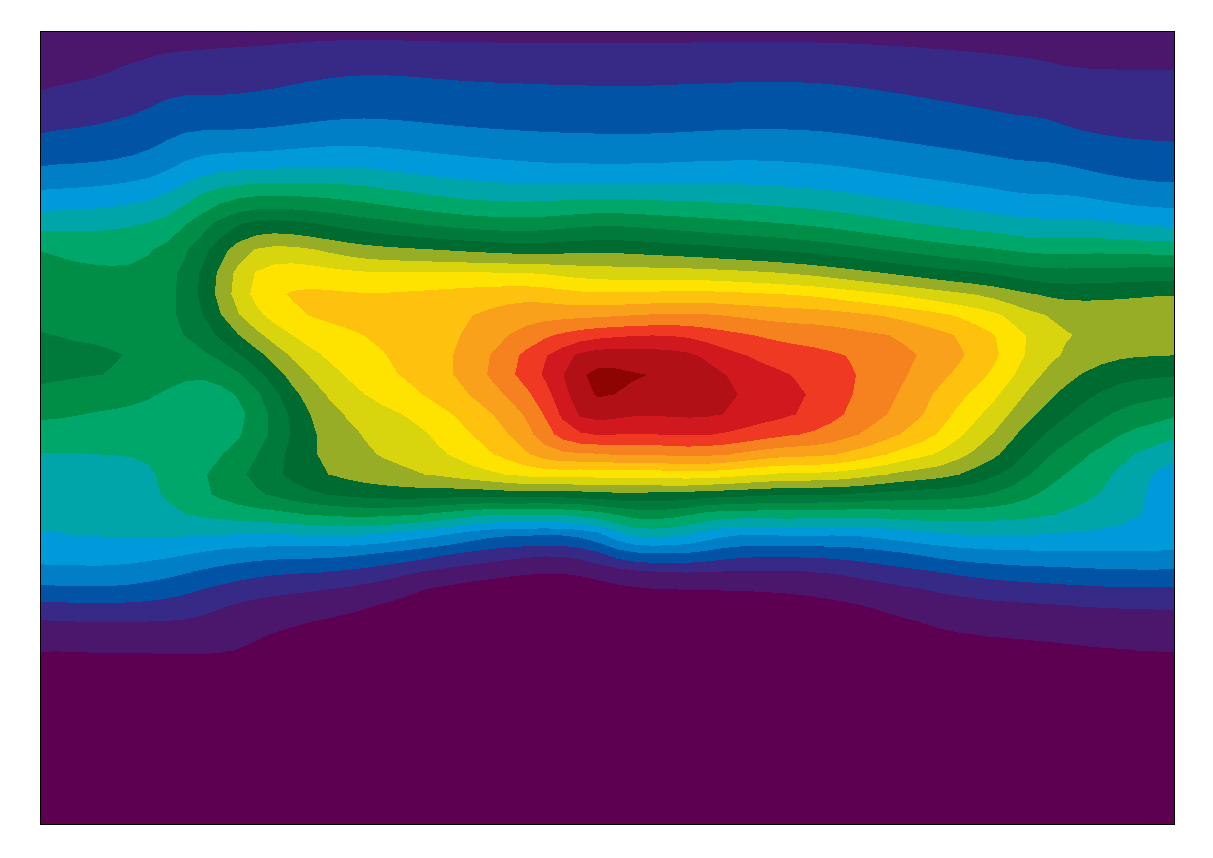
\includegraphics[width=250pt]{figures/c3manfront2}}
\put (300,250){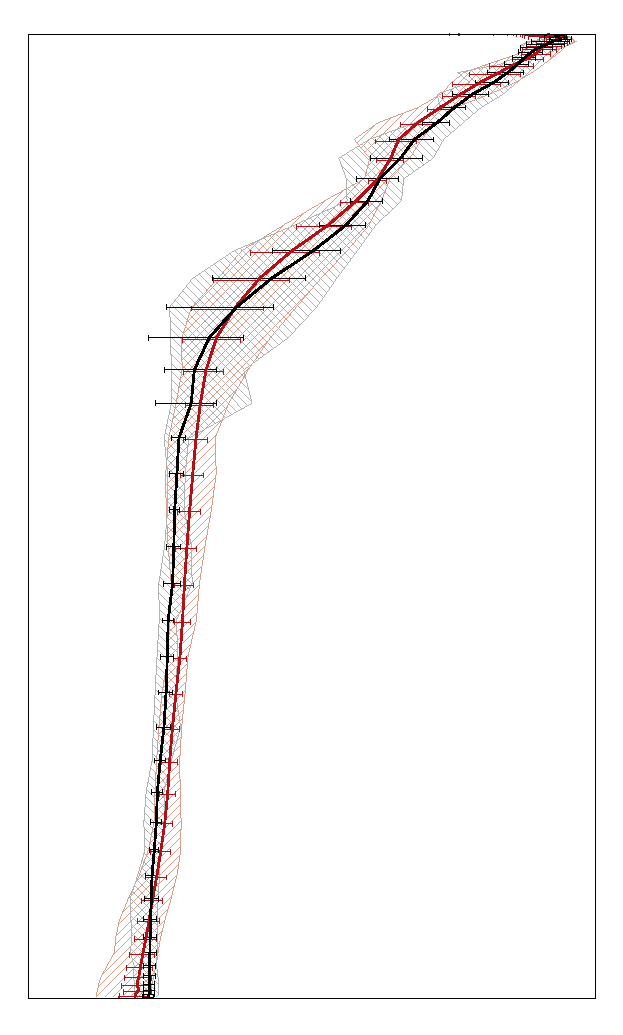
\includegraphics[width=150pt]{figures/c3manfront3}}
\end{picture}

\vspace*{24mm}
\TynnRule\\
] % end twocolumn
\clearpage
%%%%%%%%%%%%%%%%%%%%%%%%%%%%%%%%%%%%%%%%%%%%%%%%%%%%%%%%%%%%%%%%%%%%%%
%\pagestyle{plain}
\pagestyle{fancy}
\setcounter{page}{2}
\lhead{Oslo CTM3 user manual}
\rhead{\today}
\cfoot{\thepage}
\renewcommand{\headrulewidth}{0.4pt}
\renewcommand{\footrulewidth}{0.4pt}
\small
%%%%%%%%%%%%%%%%%%%%%%%%%%%%%%%%%%%%%%%%%%%%%%%%%%%%%%%%%%%%%%%%%%%%%%



%%%%%%%%%%%%%%%%%%%%%%%%%%%%%%%%%%%%%%%%%%%%%%%%%%%%%%%%%%%%%%%%%%%%%%
% Abstract -- #ABS
%%%%%%%%%%%%%%%%%%%%%%%%%%%%%%%%%%%%%%%%%%%%%%%%%%%%%%%%%%%%%%%%%%%%%%
\begin{abstract}
This manual contains a~description of the \model\ and how to set up
simulations.
Information about emissions, which type of simulation you want do,
with which components etc. are described, but most of all, this
manual attempts to document the different processes and the
source code of the \model.
\end{abstract}
%%%%%%%%%%%%%%%%%%%%%%%%%%%%%%%%%%%%%%%%%%%%%%%%%%%%%%%%%%%%%%%%%%%%%%
%%%%%%%%%%%%%%%%%%%%%%%%%%%%%%%%%%%%%%%%%%%%%%%%%%%%%%%%%%%%%%%%%%%%%%



%%%%%%%%%%%%%%%%%%%%%%%%%%%%%%%%%%%%%%%%%%%%%%%%%%%%%%%%%%%%%%%%%%%%%%
% Table of contents -- #TOC
%%%%%%%%%%%%%%%%%%%%%%%%%%%%%%%%%%%%%%%%%%%%%%%%%%%%%%%%%%%%%%%%%%%%%%
% No extra space between paragraphs is needed for TOC
\setlength{\parskip}{0mm}
% Insert table of contents
\tableofcontents
% Set space between paragraphs (to avoid using \\)
\setlength{\parskip}{3mm}
%%%%%%%%%%%%%%%%%%%%%%%%%%%%%%%%%%%%%%%%%%%%%%%%%%%%%%%%%%%%%%%%%%%%%%
%%%%%%%%%%%%%%%%%%%%%%%%%%%%%%%%%%%%%%%%%%%%%%%%%%%%%%%%%%%%%%%%%%%%%%



%%%%%%%%%%%%%%%%%%%%%%%%%%%%%%%%%%%%%%%%%%%%%%%%%%%%%%%%%%%%%%%%%%%%%%
% Introduction -- #INTRO
%%%%%%%%%%%%%%%%%%%%%%%%%%%%%%%%%%%%%%%%%%%%%%%%%%%%%%%%%%%%%%%%%%%%%%
\section{\model\ manual}\index{about the manual}
The \model\ is a~three dimensional global chemical transport model
(CTM), and this manual explains how to use it. This manual also
describes the model, and is meant as a~thorough description of
the model.

Generally, the use of the model is described in
Section~\ref{sxn:getstarted}--\ref{sxn:programming}, while the
rest is describing the different processes and the model code.

The \model\ is available through a~repository, as will be explained
in the coming sections.

First, some starting info about the \model.


% Historical background
\subsection{Historical background}\index{history}
\model\ is developed at the Department of Geosciences at the
University of Oslo (UiO), and later at the CICERO Center for International
Climate Research.
It is described by \citet{SovdeEA2012} and is an updated version of
the \oldmodel, which was based on a~CTM from University of California,
Irvine (UCI), developed by Michael Prather \& Xin Zhu (January 1996,
p-code 1.0/96), and where the chemical modules developed at the UiO
were included.

In roughly a~decade the two models diverged substantially; the
\oldmodel\ grew with additional chemistry/aerosol packages, while the
UCI group developed and improved the efficiency of the transport.
In order to save CPU hour requirements, the UCI group
(Prather {\it et al.}) updated their CTM to improve the structure,
parallelisation and transport in 2007.
Due to the large CPU requirements for the
\oldmodel, it was decided to implement the new UCI structure in the
Oslo model, earning the name \model.

By the end of 2007, the \oldmodel\ was very messy, so the update of
the core structure also initiated a~clean-up of the \oldmodel\ code.


% Version numbering
\subsection{Version numbering}
The \model\ documented by \citet{SovdeEA2012} is to be considered
version~v0.1, while the current version is \version.
Version numbering is not directly related to
repository\index{source code!repository} revision numbers,
however, in the \model\ repository, the version documented
by \citet{SovdeEA2012} was r143.

There are numerous small changes from version v0.1 to \version,
e.g.~that the aerosol packages have undergone some revisions, and
the scavenging tables have been modified.
%TOBEUPDATED
%Should include update history.


% The programming concept
\subsection{\model\ vs the UCI CTM}
During the first five years of \model\ development, the basic idea of
the \model\ was to keep the UCI model core untouched, only adding
modules we want and thereby staying away from interfering too much
with the core.

However, in 2015, the UCI CTM had already diverged some bit from the
starting point of \model, being partly rewritten to use modules
instead of common blocks.
So I decided to rewrite the \model\ into Fortran90. This was done for
all files except the transport routines, which are the basis for the
transport model. Keeping those intact may be wise in case of future
UCI updates. However, all the common blocks are now gone.

The model driver (\pmain) is kept clean and short; the \oldmodel\
philosophy that all goes into \pmain\ is left for good!

So far the \model\ changes have been large enough so it is not
possible to use the UCI chemistry just by operating a~switch.
The original UCI code files are available through the UCI group, and
will not be available in CTM3. I do, however, have their older codes
if update history is needed.

% Model limitations
\subsection{Limitations to \model}
\model\ is a good tool to study the atmospheric processes. However,
care should be taken when comparing model results with
observations. Even a~high resolution in the \model\ is actually fairly
coarse, so a~perfect fit with observations, especially close to the
Earth surface, should not be expected.

The \model\ is primarily  set up to study current meteorology, so when
using it in pre-industrial conditions you have to make assumptions.


%%%%%%%%%%%%%%%%%%%%%%%%%%%%%%%%%%%%%%%%%%%%%%%%%%%%%%%%%%%%%%%%%%%%%%
%%%%%%%%%%%%%%%%%%%%%%%%%%%%%%%%%%%%%%%%%%%%%%%%%%%%%%%%%%%%%%%%%%%%%%



%%%%%%%%%%%%%%%%%%%%%%%%%%%%%%%%%%%%%%%%%%%%%%%%%%%%%%%%%%%%%%%%%%%%%%
% Get started -- #GETS
%%%%%%%%%%%%%%%%%%%%%%%%%%%%%%%%%%%%%%%%%%%%%%%%%%%%%%%%%%%%%%%%%%%%%%
\section{Get started}
\label{sxn:getstarted}\index{get started}
%TOBEUPDATED
The \model\ is currently available through a~SVN repository (see
Section~\ref{sxn:thesource}), and to get access to the model you have
to have a~user account at the Department of Geosciences or at CICERO,
and you have to be member of the unix group \verb#gf-ozone#.
This will change eventually.

%TOBEUPDATED
I~have planned to eventually make the \model\ open source,
but that is yet for the future.

When you are well into the model, you may need some utilities or
programs (for generating e.g. input files). Such CTM-files may not be
part of the SVN, and may otherwise be located at \ctmgeopath.

Part of the SVN, though, are some tools for post processing. More of this
later.

In this Section you will find a~short description of how to download the
model from the SVN repository, a~short model overview and how to get
it running.



% How to get the model
\subsection{How to get the model -- SVN}
\label{sxn:thesource}\index{get started!get the model}\index{get started!SVN}
The \model\ is available through the UiO central subversion system
(SVN)\index{SVN}.
To access the code you have to be member of the group \verb#gf-ozone#.

SVN is a~version control system, and if you are unfamiliar with it, the
SVN book offers a~fairly good introduction to it:
{\it http://svnbook.red-bean.com/}\index{SVN!manual}.

To use SVN you need to have SVN installed/loaded. Contact your IT services
if you need help on this.

Important SVN commands are \verb#checkout#, \verb#add#, \verb#delete#,
\verb#commit#, \verb#status#, \verb#diff#, \verb#resolve# (for
versions prior to 1.5 it is called \verb#resolved#),  \verb#merge#.

You will find more about SVN in the SVN book, and a~short summary in
Appendix~\ref{app:svn}. The repository structure is described in
Section~\ref{app:repository}, where you will also see that 
there also are some plotting utilities and other tools available.


% Fetching the code
{\bf Fetching the code}\index{downloading the Oslo CTM3}
\index{SVN!fetching the code}
\index{code!where is it?}\index{source code!where is it?}\\
The code is located in
a~repository\index{source code!repository}, and you get it
by typing (in shell scripts, '\verb#\#'  allows you to write a~command
on several lines; you should skip character that and write everything
on one line):
{\small
\begin{verbatim}
svn checkout \
  svn+ssh://svn.uio.no/svnroot/osloctm3/ctm3f90 \
  <name of dir to put the code>
\end{verbatim} }
After doing this, you have a~copy of the code in the directory you
specified. In the {\it .svn} directory the original revision files are
also available, but you will not use those directly; {\it .svn} is for
SVN to use.

If you don't specify the name of directory where the code will be
copied to, it will get the repository name, i.e.~{\it ctm3f90}.


% Updating your code
{\bf Update an existing code}\index{SVN!update existing code}\\
If one of the experienced users tell you to update your code, just
go to your directory and execute the command:\\
{\small
\begin{verbatim}
svn update
\end{verbatim} }
Note that if you have modified a~file that needs update, you may
experience a~conflict\index{SVN!conflicts}, i.e.~SVN does not
understand how to merge the changes. If you are unfamiliar with this,
ask the experienced users.



% User manual
\subsection{User manual}
\label{sxn:usermanual}\index{get started!get the user manual}
The \model\ user manual (this document) is available as a~pdf~file
({\it manual\_osloctm3.pdf}) in the model directory.
The \LaTeX\ source code is located in a separate repository.


% Source code directories
\subsection{Source code directory}
\label{sxn:sourcedir}\index{source code!directory}
When you have downloaded the source code, you find that it contains
several files and some directories. The transport source codes,
i.e.~the UCI heritage of the model, are located at the top level of
the directory. Most of the files have the extension {\it .f90},
except for a~few of the transport subroutines which have extension
{\it .f}.

All the specific Oslo chemistry/physics files are put in the directory
\oslopath.
You can find more about the directory structure in
Appendix~\ref{app:repository}, and in
Appendix~\ref{app:description_of_files} you can find more information
on the files.


% Model grid
\subsection{Model grid}
\label{sxn:modelgrid}\index{model grid}\index{grid}
As already noted, the \model\ is a~global model. It is divided into
grid boxes to cover the atmosphere and hence has a~certain
resolution.
When you specify a~resolution, there are three numbers to keep in mind,
at least for ECMWF meteorology data.
The truncation number is given by 'T' (e.g.~T159), indicating the spectral
resolution of the native model (e.g.~ECMWF IFS).
The vertical resolution is given by 'L' (L60).
A~forecast model can have both gridded data and spectral data, in different
resolutions, so to define the gridded data there is the 'N' number (N80).
At ECMWF the T and N numbers are closely connected.
See Appendix~\ref{app:metdata} for more.

In the \model\ the spatial resolution is controlled by the following
parameters:
\begin{itemize2}
  \item \verb#IPAR#\index{variables!IPAR}: Number of grid boxes in
    the zonal (east-west) direction. \verb#IPARW#\index{variables!IPARW}
    is the zonal resolution of the meteorological input data and
    differs from \verb#IPAR# if you run with ``degraded'' horizontal
    resolution (see Section~\ref{sxn:degraded_res} for more on
    degradation of resolution).
  \item \verb#JPAR#\index{variables!JPAR}: Number of grid boxes in
    the meridional (north-south) direction.
    \verb#JPARW#\index{variables!JPARW} is the meridional resolution
    of the meteorological input data and differs from \verb#JPAR# if
    you run with degraded horizontal resolution (see
    Section~\ref{sxn:degraded_res} for more on degradation of
    resolution).
  \item \verb#LPAR#\index{variables!LPAR}: Number of grid boxes in
    the vertical. If you collapse layers, the vertical
    resolution of the meteorological input data is
    \verb#LPARW#\index{variables!LPARW} (see
    Section~\ref{sxn:degraded_res} for more on collapsing layers).
\end{itemize2}
There are several variables describing the grid.
The horizontal grid is set up at model start, with grid center longitudes
defined in:
\begin{itemize2}
  \item \verb#XGRD(IPAR)#\index{variables!XGRD}: Radians.
  \item \verb#XDGRD(IPAR)#\index{variables!XDGRD}: Degrees.
\end{itemize2}
And grid center latitudes:
\begin{itemize2}
  \item \verb#YGRD(JPAR)#\index{variables!YGRD}: Radians.
  \item \verb#YDGRD(JPAR)#\index{variables!YDGRD}: Degrees.
\end{itemize2}

The grid edges are defined similarly by:
\begin{itemize2}
  \item \verb#XEDG(IPAR+1)#\index{variables!XEDG}: Eastern edge
  longitude of grid box (radians).
  \item \verb#XDEDG(IPAR+1)#\index{variables!XEDG}: Eastern edge
  longitude of grid box (degrees).
  \item \verb#YEDG(JPAR+1)#\index{variables!YEDG}: Southern edge
  latitude of grid box (radians).
  \item \verb#YDEDG(JPAR+1)#\index{variables!YDEDG}: Southern edge
  latitude of grid box (degrees).
\end{itemize2}

The vertical grid, however, is not fixed throughout a~model run.
It depends on the meteorological input data, more specifically the
pressure. For a~model layer $L$, the pressure at the grid box bottom
is given by
\begin{equation}
  p_b(L) = \eta_a(L) + \eta_b(L)\,p_s
\end{equation}
where $p_s$ is surface pressure in hPa and $\eta_a$
(\verb#ETAA(LPAR+1)#\index{variables!ETAA}, units of hPa) and $\eta_b$
(\verb#ETAB(LPAR+1)#\index{variables!ETAB}, unitless)
are hybrid sigma
coordinates\index{hybrid coordinates}\index{hybrid sigma coordinates}\index{sigma coordinates}.
If you collapse layers, the original sigma coordinates are given by
\verb#ETAAW(LPARW+1)#\index{variables!ETAAW}) and
\verb#ETABW(LPARW+1)#\index{variables!ETABW}.

The grid box center pressure of a~level $L$ is halfway between the
edges of the box:
\begin{eqnarray}
  p_c(L) &=& \frac{1}{2}\left[\eta_a(L) + \eta_a(L+1)\right. \nonumber\\
                && +\left.(\eta_b(L)+\eta_b(L+1))*p_s\right]
\end{eqnarray}
The height of grid box bottoms are given by the array
\verb#ZOFLE(LPAR+1,IPAR,JPAR)#\index{variables!ZOFLE}.
Surface values of this variable act as topography, and are
calculated from a~2D annual mean surface pressure field $p_m$:
\begin{equation}
  Z_s = 16000\log10\left(\frac{1013.25\textrm{hPa}}{p_m}\right)
\end{equation}
The height levels above the surface (i.e.~for the vertical range
\verb#2:LPAR+1# of \verb#ZOFLE#) are calculated from the thickness
of each layer, based on temperature ($T$), specific humidity ($q$) and
pressure at grid box edges ($p_b$).
\begin{eqnarray}
  \Delta Z(L) &=& -29.27 T(L)\left[1-0.6q(L)\right] \nonumber \\
           && \cdot \log\left(\frac{p_b(L+1)}{p_b(L)}\right)
\end{eqnarray}
Although $Z_s$ is the topography in meters, this quantity is mainly
used for diagnostics. Physical processes generally use \verb#ZOFLE# to
find layer thickness, while it is the surface pressure that defines
the topography.
See Appendix~\ref{app:layerheights} for some more info.



% Degraded resolution
\subsubsection{Degraded resolution}
\label{sxn:degraded_res}\index{setup!resolution}\index{resolution!degraded}\index{degraded resolution}
The \model\ can be run with lower resolution than the meteorological
input data. It is possible to collapse as many layers as you like,
however, \makefile\ allows for only one automatic set-up, collapsing
layer 1--3 and 4--5 into two layers. See Section~\ref{sxn:makefile}
for \makefile\ user settings. While this is standard treatment by the
UCI~group, the \model\ has so far not  been used in this fashion.

A~newer feature to \model\ is that the horizontal resolution may be
degraded, combining e.g.~4 boxes into one. This means that the model
can read e.g.~1.125$^{\circ}$\,x\,1.125$^{\circ}$ meteorological data, and convert
them to 2.25$^{\circ}$\,x\,2.25$^{\circ}$ resolution, but still using
the native resolution for calculating cloud properties.
The \makefile\ settings are:
\begin{itemize2}
  \item \verb#HWINDOW=HORIGINAL#: Use native resolution.
  \item \verb#HWINDOW=HTWO#: Combine 2\,x\,2 native boxes.
  \item \verb#HWINDOW=HFOUR#: Combine 4\,x\,4 native boxes.
\end{itemize2}
Also described in Section~\ref{sxn:makefile}.


% Oslo CTM2 vs Oslo CTM3
\subsection{\model\ vs \oldmodel}
\label{sxn:o3vso2}\index{OsloCTM2 vs OsloCTM3}\index{CTM2 vs CTM3}
Skip this part if you are not familiar with \oldmodel.

The structure of the model has changed substantially since \oldmodel.
In the \oldmodel\ all tracers were located in the tracer array
\verb#STT#\index{variables!STT}, whereas
in \model\ only the transported tracers are in \verb#STT#. Therefore
also \verb#MTC#\index{variables!MTC} is now only for the transported
species. Other variables have also been changed to separate the
transported and non-transported species.
The non-transported species are stored in \verb#XSTT#, and will be
further explained in Section~\ref{sxn:sourcecode}.

The parallel structure has changed, and most processes (chemistry,
boundary layer mixing, emissions, etc.) are now integrated columnwise
instead of through a~latitude band. Horizontal transport, however, is
calculated layer by layer (see Section~\ref{sxn:transport}).
Section~\ref{sxn:sourcecode} describes the source code more closely.


{\bf Input files and diagnostics}\\
The diagnostics have changed, as well as the names of the input
files. The input files are described in Section~\ref{sxn:setup}, while
diagnostics are described in Section~\ref{sxn:diagnostics}.

{\bf C-code}\\
The C-coding in the \oldmodel\ has been removed, and replaced with
dummy calls and logical switches. This will be explained thoroughly in
this manual.

{\bf Changes in chemistry}\\
There are some changes in the tracer list since \oldmodel:
\begin{itemize2}
  \item Tracer number 2 (\verb#NOX#), the sum of NOx components (NO,
    NO$_2$, NO$_3$, 2xN$_2$O$_5$+PAN) is only set in the tropospheric
    chemistry for stability. There is no need to transport NOX since
    all its components are transported.
  \item Tracer number 3 (\verb#NOZ#), the sum of NO$_3$ and N$_2$O$_5$
    is removed. It is now set in the tropospheric chemistry, as was
    done already in the stratospheric chemistry. NOZ is treated in
    chemistry to create stability, and does not need to be transported
    as long as NO$_3$ and N$_2$O$_5$ are transported.
  \item Tracer number 26 (\verb#CH2O2OH#) was transported but not
    used. It is removed.
  \item Tracer number 45 (\verb#O3NO#) is
    set inside the tropospheric chemistry from O$_3$ and NO, also for
    stability. It was not transported, not used in the stratosphere,
    and the diagnose was not useful, therefore it was removed.
  \item Tracer number 47 (\verb#DMS#) is not in use in the
    tropospheric chemistry, and is removed. It is used in the sulphur
    scheme where it has a~new number (which is 71).
\end{itemize2}

% NPAR
{\bf NPAR}\index{variables!NPAR}\\
In contrast to the \oldmodel\ the \verb#STT#\index{variables!STT} now
{\it only handles the transported species}, given by
\verb#NPAR#. Non-transported species are treated as a~separate
array \verb#XSTT#\index{variables!XSTT}, of which there are
\verb#NOTRPAR#\index{variables!NOTRPAR}.
See Section~\ref{sxn:coresource} for more on this.

% Convective activity
{\bf Convective activity}\index{convective activity files}\\
The convectivity files used for lightning emission in \oldmodel\ are
not needed in the \model. This is because the lightning routine is now
more consistent with the meteorological data, not using the
\citet{PriceEA1997a} dataset.

In the \model\ we calculate a~somewhat similar convective activity at
each time step and scale it against a~climatological mean. This mean
is specific for a~certain meteorological dataset, and is sensitive
for resolution.
An important difference to the \oldmodel\ is that the
\oldmodel\ divided the annual amount following the monthly totals of
\citet{PriceEA1997a}, whereas \model\ more physically follows only
the meteorological conditions.
It could be noted that \citet{MurrayEA2012} argue that Northern
Hemisphere summer lightning produce more NOx than elsewhere and at
other seasons, but this is not included in \model.
See Section~\ref{sxn:emissions_lightning} for more on lightning
emissions.

% fast-JX
{\bf fast-JX}\\
The Fast-J2 \citep{BianPrather2002} applied in the \oldmodel\ has been
replaced by fast-JX in the \model. There are some differences in the
photochemistry, e.g.~slight differences in cross sections.


% Source code documentation
{\bf Source code documentation}\\
In the process of cleaning up the Oslo code, also the source code
comments have been revised and improved. See
Section~\ref{sxn:programming} for programming guidelines.

% Variable names
{\bf Variable names}\index{variables}\index{variable names}\\
There are several variable names that have been renamed from
\oldmodel\ to \model. The new variable names are more self-explaining.

A~good example of a~changed variable name is the tropopause level,
which is now called \verb#LMTROP#\index{variables!LMTROP}, since it is
the ``\verb#LM# of the troposphere''. In the old model its name was
\verb#LMSTRT#, which was somewhat misleading.

Another is the max number of component IDs, which has been changed
from \verb#IREPMX# to
\verb#TRACER_ID_MAX#\index{variables!TRACER\_ID\_MAX}.

The tracer mapping from chemical id to transport number has changed
name from \verb#MTC# to
\verb#trsp_idx#\index{variables!trsp\_idx}.
Similarly, the mapping the other way is changed from \verb#IDMTC# to
\verb#chem_idx#\index{variables!chem\_idx}.

\verb#TMMVV#, the conversion factor from mass mixing ratio to
volume mixing ratio, is called
\verb#TMASSMIX2MOLMIX#\index{variables!TMASSMIX2MOLMIX}.
There are also mappings the other way, namely
\verb#TMOLMIX2MASSMIX#\index{variables!TMOLMIX2MASSMIX}.

Old variable names are not listed in the index list, so if you wonder
where to find the old variable, ask the experienced users.

% Other differences
{\bf Other differences}\\
In the \oldmodel\ the whole tracer array (\verb#STT#) was often
converted from one unit to another unit, just to access a~few tracers
in the correct units. This is no longer possible, and should be
avoided.

Other differences are noted when necessary in the other sections.



% Variable names
\subsection{Variable names}
\label{sxn:variable_names}\index{variables}\index{variable names}
Most of the model variable names referred to in this manual are listed
in the index list at the end of the manual, under ``variables''.
If you cannot find the variable names there, they are probably not
mentioned here, and you have to look in the model files. A~good place
to start is the global variables in the files called \verb#cmn_*# (cmn
for common files instead of common blocks).

If you look for a~variable and do not find it in the indexed list, you
may also do a~text search in this document; the variable may not have
been included in the index list.



% Setting up the model - Special/important files
\subsection{Setting up the model}
\label{sxn:setup}\index{setup}\index{model setup}
This section will explain the steps to get the model running, and will
describe some important files.

You need to know the
\begin{itemize2}
  \item Makefile
  \item pmain.f90
  \item input file (\maininput), which lists some important flags and
    input file names.
  \item tracer list (\tracerlist)
  \item wet scavenging list (\wetscavlist), which lists how to treat
    wet scavenging of tracers.
  \item dry scavenging list (\dryscavlist), which lists how UCI treats
    dry deposition of tracers. NOT used for Oslo chemistry! Oslo
    chemistry uses the file \dryscavlistOC, located in the directory
    \inputctmiii.
  \item meteorological data
  \item other input data, e.g.~how to treat CH$_4$ at the surface
    (and possibly how to initialize the tracer array
    \verb#STT#\index{variables!STT}).
\end{itemize2}


% Makefile
\subsubsection{\makefile}
\label{sxn:makefile}\index{setup!Makefile}\index{Makefile}
The first file you need to know, is the \makefile.
In \makefile\ you can set user options, i.e.~which modules or packages
to apply, which resolution to use and some compiler options. Your
choices are:
\begin{itemize2}
  \item \verb#OPTS#\index{Makefile!OPTS}: Optimize
    (\verb#O#, \verb#A#) or debug (\verb#D#).
  \item \verb#HNATIVE#\index{Makefile!HNATIVE}: Horizontal resolution of
    meteorological data, e.g. T42, T159.
  \item \verb#VNATIVE#\index{Makefile!VNATIVE}: Vertical resolution of
    meteorological data, most likely L60, but old files exist in e.g. L40.
  \item \verb#HWINDOW#\index{Makefile!HWINDOW}: Model degradation of
    horizontal resolution. Setting it to \verb#HORIGINAL#, the model uses
    native resolution, and with \verb#HTWO# it combines 2\,x\,2 native
    grid boxes. A~third option is \verb#HFOUR#.
  \item \verb#COLLAPSE#\index{Makefile!COLLAPSE}: Collapse layer 1-3
    and 4-5 into two layers.
  \item \verb#OSLOCHEM#\index{Makefile!OSLOCHEM}: Turn on Oslo
    chemistry/physics. For \model\ you would most likely never turn
    this off.
  \item \verb#TROPCHEM#\index{Makefile!TROPCHEM}: Oslo
    tropospheric chemistry (Section~\ref{sxn:tropchem}).
  \item \verb#STRATCHEM#\index{Makefile!STRATCHEM}: Oslo
    stratospheric chemistry (Section~\ref{sxn:stratchem}).
  \item \verb#SULPHUR#\index{Makefile!SULPHUR}: Sulphur
    chemistry and sulphate (Section~\ref{sxn:sulphur}).
  \item \verb#BCOC#\index{Makefile!BCOC}: Black and organic
    carbon package (Section~\ref{sxn:bcoc}).
  \item \verb#NITRATE#\index{Makefile!NITRATE}: Nitrate package
    (Section~\ref{sxn:nitrate}).
  \item \verb#SEASALT#\index{Makefile!SEASALT}: Sea salt package
    (Section~\ref{sxn:salt}).
  \item \verb#DUST#\index{Makefile!DUST}: Mineral dust package
    (Section~\ref{sxn:dust}).
  \item \verb#SOA#\index{Makefile!SOA}: Secondary organic aerosols package
    (Section~\ref{sxn:soa}).
  \item \verb#E90#\index{Makefile!E90}: Turn on to use e90~tracer for
    STE flux calculations (Section~\ref{sxn:ste}) and to produce the
    tropopause
    \verb#LSTRATAIR_E90#\index{variables!LSTRATAIR\_E90}\index{variables!LPAUZ|see {LSTRATAIR\_E90}}
    (not yet used to distinguish tropospheric and stratospheric chemistry).
  \item \verb#LINOZ#\index{Makefile!LINOZ}: Turn on to use Linoz~O$_3$
    for STE calculations.
    \model\ has not yet been set up to use Linoz to replace
    stratospheric chemistry.
  \item \verb#LIT#\index{Makefile!LIT}: Can be used for generating
    lightning factors. Explanation is given in \makefile.
  \item \verb#EMISDEP_TREATMENT#\index{Makefile!EMISDEP\_TREATMENT}:
    Defines whether to treat emissions and deposition as separate
    processes (\verb#EMISDEP_TREATMENT :=U#) or as respectively
    production and loss in chemistry (\verb#EMISDEP_TREATMENT :=O#).
  \item \verb#FC#\index{Makefile!FC}: Fortran compiler (\verb#ifort#,
    \verb#pgf90#, \verb#openf90# ...) See Appendix
    \ref{app:compiler} for more on the compiler options.
\end{itemize2}


\makefile\ does {\it not} use a~dependency
generator\index{dependency generator}, so if you add files to be
compiled you have to add dependency rules at the end of \makefile.
How to do this is described closer in Appendix~\ref{app:makefile}.

The \makefile\ tokens set up the compilation and is used for setting
model parameters. The file
{\it cmn\_size.F90}\index{cmn\_size.F90|see {source code}}
is the only file (except the mineral dust code) containing C-style code, and
thereby needs to be preprocessed by the Fortran compiler.

See Section~\ref{sxn:getstarted_compiling} if you don't know how to
compile.

If you want to run non-standard resolutions, you need to check
that the {\it cmn\_size.F90} has the necessary parameters.

See Appendix~\ref{app:makefile} for more on \makefile.





% pmain
\subsubsection{Main program -- \pmain}
\label{sxn:pmain1}\index{setup!pmain}
The main program is located in \pmainf. It is described in
Section~\ref{sxn:structure}. You should know the structure of \pmainf, 
and how it works. When you need to work on the tracer arrays, you
should also know how the parallel regions work.




% main input file
\subsubsection{Input file -- \maininput}
\label{sxn:maininput}\index{setup!main input file}
There is one input file for each resolution, and it is typically
called \maininput.
The first part of the file is to set up the run, with information
about the date, time steps, meteorological fields, and physical
processes (boundary layer mixing, dry and wet deposition schemes).

The second part lists some input file names, e.g. the tracer list
file (\tracerlist), while the third part covers information about the
diagnostics (covered in Section~\ref{sxn:diagnostics}).

The important parameters to set are
\begin{itemize2}
  \item{\verb#IYEAR#}: Reference year.
  \item{\verb#NDAYI#}: Day of year to begin CTM run.
  \item{\verb#NDAYE#}: Day at end of CTM run (finishes at end of
    day \verb#NDAYE-1#).
  \item{\verb#LCLDQMD#}: Use mid-point of quadrature cloud cover
    independent cloud atmospheres (ICA\index{ICA, independent column
      atmosphere}\index{independent column atmosphere (ICA)}) (for
    fast-JX, Section~\ref{sxn:cloudcover}\index{variables!LCLDQMD}).
  \item{\verb#LCLDQMN#}: Mean quadrature cloud cover
    ICAs\index{variables!LCLDQMN} (for fast-JX).
  \item{\verb#LCLDRANA#}: Random selected from all cloud cover
    ICAs\index{variables!LCLDRANA} (for fast-JX; default treatment).
  \item{\verb#LCLDRANQ#}: Random selected from 4 mean quadrature cloud
    cover ICAs\index{variables!LCLDRANQ} (for fast-JX).
  \item{\verb#RANSEED#}: The seed number to create random
    numbers. Ensures that the random cloud properties are the same in
    two runs\index{variables!RANSEED}).
  \item{\verb#NROPSM#}: Number of operator split steps per
    meteorological time step. Default is 1\,hour,
    i.e.~\verb#NROPSM=3#\index{variables!NROPSM}.
    Note that the meteorological steps per day
    (\verb#NRMETD#\index{variables!NRMETD}) is hard coded into the model
    because it is necessary for e.g. the diagnostic tools.
  \item{\verb#NRCHEM#}: Number of chemical sub steps per operator
    split step. Default is \verb#NRCHEM=1#\index{variables!NRCHEM}.
  \item{\verb#LJCCYC#}: Flag for calculating J-values every internal
    chemical cycling step\index{variables!LJCCYC}. See Section
    \ref{sxn:photochemistry} for more.
  \item{\verb#LMTSOM#}: Second order moment limiter\index{variables!LMTSOM}.
    Should be~2 (monotonic), but can also be set to~1 () and~3 (min/max).
    Do {\bf not} change this unless you know what you are doing.
  \item{\verb#CFLLIM#}: Global CFL limit \index{variables!CFLLIM} for
    divergence, i.e. max allowed amount taken from a~grid box in
    advection. This value should be set to 0.95, and you should not need
    to change it. With the \oldmodel\ there were a~few instances where
    certain meteorological data would cause the model to crash because
    0.95 was too high, this behaviour has so far not been seen in \model.
\end{itemize2}

Next, there is a~section for meteorological data, specifying which type of
data and where to read them:
\begin{itemize2}
  \item{\verb#metTYPE#}: Possible types\index{variables!metTYPE} are
    \verb#ECMWF_oIFS# for OpenIFS generated locally at CICERO/UIO, and
    \verb#ECMWF_IFS# for the IFS data generated at ECMWF/UIO.
  \item{\verb#metCYCLE#}: The cycle\index{variables!metCYCLE} of the
    ECMWF IFS/OpenIFS model.
  \item{\verb#metREVNR#}: The revision number\index{variables!metREVNR} of
    the ECMWF IFS/OpenIFS model.
  \item{\verb#LLPYR#}: Allow for leap\index{variables!LLPYR} year.
  \item{\verb#LFIXMET#}: Annually recycle met fields\index{variables!LFIXMET}.
  \item{\verb#JMPOLAR#}: Defines\index{variables!JMPOLAR} if polar grid box
    has same latitudinal size as other grid boxes (\verb#JMPOLAR=0#) or half
    size (\verb#JMPOLAR=1#). Should be 0 for ECMWF data.
  \item{\verb#GM0000#}: I-coord of Greenwich Meridian\index{variables!GM0000}.
    For ECMWF \verb#GM0000=1.5#, meaning that Greenwich (0$^{\circ}$E) is
    in the middle of grid box~1 (so that 1 is left edge and 2 is right edge).
    Other meteorological data may have different grids.
\end{itemize2}

After this, the hybrid sigma
coordinates\index{hybrid coordinates}\index{hybrid sigma coordinates}\index{sigma coordinates}
are listed. Note that if you collapse layers (\verb#COLLAPSE# in \makefile),
the \verb#LMMAP#\index{variables!LMMAP} must match this. So if you collapse
layers 1--3, the \verb#LMMAP# of the first 3~entries must be 1.
Native level~4 will then have \verb#LMMAP=2#. Traditionally, the \model\
had always been run in native vertical resolution, while UCI-CTM is
often run with collapsed layers near the surface.

Next:
\begin{itemize2}
  \item{\verb#PFZON#}: Allows polar latitudes to combine grid boxes
    horizontally\index{variables!PFZON}. However, this is not applied
    in \model. Entries should therefore be~1 (there are 25 entries).
  \item{\verb#NBLX#}: Boundary layer scheme\index{variables!NBLX} (Section
    \ref{sxn:transport_blmix}). Default should be~5.
  \item{\verb#NDPX#}: Dry deposition scheme\index{variables!NDPX} (Section
    \ref{sxn:drydep}). Only simple UCI scheme is available, but it is
    modified/overwritten for the \model.
  \item{\verb#NSCX#}: Scavenging scheme for large scale
    scavenging\index{variables!NSCX} (Section
    \ref{sxn:ls_scav}). Should be set to~1.
\end{itemize2}


Then input filenames for annual mean pressure and vegetation are
listed, followed by  more tracer specific parameters, e.g.~how to
start the model:
\begin{itemize2}
  \item \verb#LCONT#: Start from restart file (\verb#T#) or not
    (\verb#F#)\index{variables!LCONT}.
  \item \verb#START_AVG#\index{variables!START\_AVG}:
    If \verb#LCONT = F#, this index specifies how else to initialize
    the tracer field. \verb#START_AVG=0#: \verb#STT=0#,
    \verb#START_AVG=1#: start from \model\ average file.
\end{itemize2}

A chemistry run initialised to zero (\verb#LCONT=F# and
\verb#START_AVG=0#) will crash, probably reporting negative
stratospheric NO$_x$ or NO$_y$.

In this tracer specific section, the filenames of the tracer list
(Section~\ref{sxn:tracerlist}), scavenging lists and emission list
(Section~\ref{sxn:emisfile}) are given.

Note that the tracer list is read immediately after it is defined.
This is to allow for checking against included tracers, e.g.~by
different diagnostics.

Lastly, there are several settings and flag calendars for
diagnostics.
\begin{itemize2}
  \item \verb#JDO_C#\index{variables!JDO\_C}: When to save restart files.
  \item \verb#JDO_T#\index{variables!JDO\_T}: When to do tendencies.
\end{itemize2}
With the tendency tracer flags you specify which tracers to
diagnose. Note that these are transport numbers, not component IDs.

Then we have:
\begin{itemize2}
  \item \verb#JDO_A#\index{variables!JDO\_A}: When to do averages.
  \item \verb#JDO_X#\index{variables!JDO\_X}: When to do STE calculations.
\end{itemize2}

And finally the UCI time series output.
This is not the same as the \model\ time series
(Section~\ref{sxn:vprofseries}), and is not used.

%TOBEUPDATED
{\bf Future update}\\
Using transport numbers to define output is problematic, because you need
to keep track of the order of components. In the future this will be changed
to component names.





% Tracer list
\subsubsection{Tracer list -- \tracerlist}
\label{sxn:tracerlist}\index{setup!tracer list}
\index{setup!tracer\_list.d, tracer list}\index{tracer\_list.d, tracer list}
\index{tracer list, tracer\_list.d}
The tracer list (\tracerlist) lists all tracers needed in the
simulation.
Names and molecular weights are listed, as well
as some diagnostic flags {\it that are not yet in use}.

The list is divided into two parts: the first lists the transported and
the second lists the non-transported species.
The total listed numbers of transported and
non-transported species must match \verb#NPAR# and \verb#NOTRPAR# in
{\it cmn\_size.F90}.

When read into the model, the tracer names are found in the variables
\verb#TNAME#\index{variables!TNAME} for transported species and
\verb#XTNAME#\index{variables!XTNAME} for non-transported species.

There may be a~tracer list available for your choices,
and they are located in the directory {\it tables}.
You may have to make your own tracer list, depending on which applications
you include.

It can be mentioned that eventually, the non-transported array should be
removed, but this is left for future work.

{\bf Where is the tracer list specified?}\\
The path and file name of the tracer list is specified in the
input file \maininput.



% Emissions list
\subsubsection{Emissions list -- \emisfile}
\label{sxn:emisfile}\index{setup!emissions list}
\index{setup!Ltracer\_emis.inp, emissions list}\index{emissions list, Ltracer\_emis.inp}\index{Ltracer\_emis.inp}
This file contains all emission information needed for the \model\ to
run; information on forest fires, lightning, 2D and 3D monthly
emissions.
The files are located in the directory \emislistdir. You may want to
build your own list; just save it under a~different name.
There are files for different main inventories, such as
CEDS, ECLIPSE, RETRO and Lamarque, listed in the subdirectory
{\it EMISSION\_LISTS}.

The most recent dataset is CEDS (CMIP6) version from May 2017.

{\it Important~1}:\\
You should keep good track of the emission inputs you use in different
model runs; they are important to be able to reproduce the simulations.
For simplicity, the whole list is printed to standard out, before
reading the file again and doing the actual read-in of emission datasets.

{\it Important~2}:\\
There is not really a default/preferred emission dataset yet, so you have
to ask the experienced users about which you should use. It will
probably be best to use the newest emission estimates.
There are several datasets for anthropogenic emissions, but fewer for
natural emissions.
Natural emissions will often have to be taken from several datasets.

{\it Important~3}:\\
If you want to include CH$_4$~emissions instead of using
the standard fixed surface concentrations, you have to do some changes
to the code and input files. To do this correctly, you {\bf must} read
Section~\ref{sxn:emissions_ch4}.

{\it Important~4}:\\
If you want to build your own emission list, please read 
Section~\ref{sxn:emissions_howto}.

File names of emission files are listed along with scaling for each
component which the file applies for. Also a~few short term variations
can be specified.

Note that the whole path for the emission files should be given in
the emission list (\emisfile), so you don't have to link to the
emission directory.

Emission data can usually be found in a~directory available for all
users. However, when you start using the
\model, you should ask us where to find the data.

See Section~\ref{sxn:emissions} for further information on the
emissions and the scaling possibilities.




% Meteorological data
\subsubsection{Meteorological data}
\label{sxn:metinfo}\index{setup!meteorological data}\index{meteorological data}
Traditionally, the \model\ has been driven by meteorological data from
the ECMWF Integrated Forecast System (IFS) model, in both 40-layer and
60-layer versions.
In 2015, the ECMWF openIFS model was applied to generate new data locally
at CICERO/UIO, covering a~larger time period. This model is in principle
similar to the IFS model.

You define which meteorological data to use in the file \maininput.
First you need to specify the dataset:
\begin{itemize2}
  \item \verb#metTYPE#\index{metTYPE}\index{meteorological data!metTYPE}:
    Which type of data. \verb#ECMWF_oIFSnc4# is openIFS data in
    netCDF4 format. \verb#ECMWF_oIFS# is openIFS data in the UIO format.
    \verb#ECMWF_oIFS# is the older IFS data in the UIO format.
  \item \verb#metCYCLE#: The cycle number of the model used to generate
    meteorological data.
  \item \verb#metREVNR#: The revision number of the cycle version.
\end{itemize2}
Note that the \model\ is only set up for these datasets so far.
When other data is used, a~new read-in routine must be made, and then
the cycle and revision numbers can still be used to define the
model version.

Next you define the path where the meteorological data is located, 
\verb#MET_ROOT#\index{variables!MET\_ROOT}.
The \model\ will use \verb#metTYPE#, \verb#metCYCLE#, \verb#metREVNR#
and \verb#metTYPE# to make the full path of file names.
This is carried out in the \verb#INPUT# routine in file
{\it initialize.f90}.

When you start using the \model, you should ask current users where to
find the data.

{\it Important}\\
The openIFS meteorological data was updated from binary files to netCDF4
files late 2015. You can find more about the meteorological data and the
data formats in Appendix~\ref{app:metdata}.
If you need to run the old format, there is a~separate
read-in available, called {\it metdata\_ecmwf\_uioformat.f90}.
The \model\ should give you a~hint about this if you specify an old
\verb#metTYPE#.


{\it Important for older meteorology data}\\
The old format will eventually be phased out. The new format has greater
flexibility e.g.~to read a~field from the next time step and interpolate
temporally between them. If that is included at some point, it will be
difficult to use the binary files.

If you get very strange results in the first time steps, you may have
chosen the wrong resolution data. Reading 60-layer data in a~L40
model run, may not proceed past the end of the file. But a~L60 run will
try to read past the end of file of 40-layer data, and the model will
crash.


% Restart file
\subsubsection{Restart file}
\label{sxn:restartfile}\index{setup!restart file}\index{restart file}
A~restart file contains tracer distributions for all species in
a~simulation, as well as the moments for all the transported species.
It allows you to continue a~run without loss of tracer information,
and while some aerosol packages can be started from zero, chemical
components usually requires initial values.


There are several versions of read-in routines available. The standard
read-in reads netCDF4 files, and is called
\verb#load_restart_file#\index{subroutines!load\_restart\_file},
located in the file
{\it stt\_save\_load.f90}\index{source code!core!stt\_save\_load.f90}.
It is called from subroutine
\verb#SETUP_SPECIES#\index{subroutines!SETUP\_SPECIES} in the file
{\it initialize.f90}\index{source code!core!initialize.f90}, which is
is called from \pmainf.

In the restart file, transported species have prefix \verb#STT_#,
and for these species there are also moments available, having
prefixes
\verb#SUT_#, \verb#SVT_#, \verb#SWT_#, \verb#SUU_#, \verb#SVV_#,
\verb#SWW_#, \verb#SUV_#, \verb#SUW_#, \verb#SVW_#.
Non-transported species have prefix \verb#XSTT_#.

The read-in will interpolate horizontally if the model resolution
differs from the file resolution, but note that in such cases only
two moments are used: \verb#SWT# and \verb#SWW_#.

%TOBEUPDATED
A~possibility for vertical interpolation should be included eventually.

The read-in assumes the restart file is called {\it restart.nc}, but
note that it is possible to read several restart files. As long as
the read in flag \verb#MODE#\index{variables!MODE} is set correctly,
only the uninitialised fields will then be set.

Complementary, there is a~routine to save the restart files, called
\verb#save_restart_file#\index{subroutines!save\_restart\_file},

As a~new user, you should regularly check that you actually use the
restart file you think you use.

Traditionally you can also restart from a~monthly average, but this
needs more spin-up. There is yet no routine for reading average netCDF
files.




% Other input data
\subsubsection{Other input data}
\label{sxn:otherinput}\index{setup!linking to input data?}\index{linking to input data?}\index{setup!input data}\index{input data}
There are some additional data you need for running the \model. The
model reads these data from the directory \inputctmiii, so you
need to link to that directory. On the Abel cluster this is located at
\hpcdatageo{\it /}\inputctmiii, and the data consists of
\begin{itemize2}
  \item 2d-data for the stratospheric module (boundary condition
    data).
  \item Background aerosol surface area densities for the
    stratospheric module.
  \item CH$_4$ surface mixing ratios.
  \item Dry deposition values.
\end{itemize2}


% 2D-data
{\bf 2d-data}\index{2d-data}\index{stratospheric chemistry!2d-data}\\
Stratospheric chemistry includes a~number of species which have
long tropospheric lifetimes, and thus is set as fixed mixing ratios
in the model levels closest to the surface.
At the top of the model, i.e. upper stratosphere, the model lacks
information on how much is transported upwards (into the mesosphere)
and also on mixing ratios to be transported downwards (from the
mesosphere).

Species having very long lifetimes and are destroyed in the mesosphere,
they may build up in the stratosphere if the flux out is not considered.
Likewise, if a~component is produced in the mesosphere and transported
downwards, it would not be included as a~source for the stratosphere.

Traditionally, upper boundary conditions have been set for
many species, mimicking this, while doing chemistry up to the 
next-to-uppermost layer (\verb#LPAR-1#).

These boundary conditions are taken from simulations done with
the Oslo 2D\index{Oslo 2D} model, and are just called the 2d-data.
The data are read from the directory \inputctmiii, so you have
to link this directory to where you run the model.

While such a~method may hinder build-up of some species, it
is for other species not an ideal solution.
\begin{itemize2}
  \item Firstly; the uppermost level of the 2D model is about 55\,km,
    well below the L60 top level. The mixing ratios are therefore scaled
    to the L60 vertical grid using the uppermost mixing ratio gradient
    of the 2d-data (see Section~\ref{sxn:stratchem_lparchem} for more).
    Using 2d-data may perhaps be OK for L40, but not for L60.
  \item Secondly; depending on the tracer, it may effectively act as
    either a~sink or a~source. This may not be what was intended.
  \item A~third obstacle is that upper boundary conditions must match
    the simulated year. Removing it will make modelling e.g.
    pre-industrial and future atmospheres easier.
  \item Finally, the Oslo~2D model can no longer be run because its
    input files are nowhere to be found. The 2D data are therefore not
    available for years after 2011.
\end{itemize2}
One solution is to use e.g. WACCM to produce boundary conditions.
Another, perhaps better, solution is to do chemistry all the way
p to the model top, so that there is a~fixed lid on top of the model.
If a~flux out or in is needed, it should be parameterised as a~separate
process.
%TOBEUPDATED
{\bf I~am currently trying to revise this (started January 2015).}


The 2d-data are read from original Oslo 2D files, so-called
{\it sr-files}, and interpolation to model resolution is carried out
on-line.





% Background aerosol surface area density
{\bf Stratospheric background aerosols}\index{background aerosols!stratosphere}\\
Background aerosol surface area density is important for the
heterogeneous chemistry\index{heterogeneous chemistry} in the
stratosphere. These data are also located in
the directory \inputctmiii{\it{/backaer\_monthly/}}.

These data were compiled by David Considine and Larry Thomason at NASA
LaRC, based on SAGE II, SAGE I and SAM II satellites. Data was
prepared by the approach of \citet{ThomasonEA1997}, and
a~description can be found in the {\it backaer\_monthly/} directory.

The data are read from the original resolution and interpolated
on-line to the model resolution.

Only year 1979 to 1999 are available, where 1979 is used for all years
prior to 1979 and 1999 for all years after 1999.




% Dry deposition
{\bf Dry deposition}\index{dry deposition!input data}\\\
Dry deposition velocities are read from the~file {\it drydep.ctm}, which
is found in the \inputctmiii\ directory.
A~new dry deposition scheme is under way, and will replace this method
or most species. See Section~\ref{sxn:drydep} for more.



% Surface CH4
\subsubsection{Surface CH4}
\label{sxn:surface_ch4}\index{setup!surface CH$_4$}\index{surface CH$_4$}\index{CH$_4$ fixed at surface}
Due to its long lifetime, CH$_4$ is usually fixed at the model
surface. This is the default treatment in \model.
The files containing this input data are located in the
\inputctmiii\ directory. Surface volume mixing ratios
were calculated in the project HYMN, where CH$_4$ emissions were
included, and monthly averages for 2003, 2004 and 2005 are available
for \model. Currently we use 2003 monthly values, however, these values
should be scaled to match observed values for the year you are simulating.
This can be done by a~separate routine, scaling the HYMN 2003 dataset
to marine global annual CH$_4$ observed by ESRL Global Monitoring Division
(see Section~\ref{app:ch4routines}).


{\bf Important 1}\\
For pre-industrial simulations, these will have to be scaled or
updated.\index{setup!pre-industrial CH$_4$}\index{pre-industrial surface}\index{pre-industrial emissions}

To match these surface values, it is possible to also set the whole 3D
tracer field from the HYMN results.\index{CH$_4$!3D initialisation}


{\bf Important 2}\\
As noted above, the fixed CH$_4$ field from HYMN can be scaled to observed
values. If you use a~CH$_4$ field from a different year, you can make
a~similar scaling routine (see Appendix~\ref{app:ch4routines}).


{\bf Not so important}\\
Also available are RETRO surface values, as zonal means for different
years.


{\bf CH$_4$ emissions}\index{setup!surface CH$_4$ emissions}\\
The \model\ can also be run with CH$_4$ surface emissions. Currently
the possible set-up is a~combination of anthropogenic emissions and natural
emissions and soil uptake provided by Bousquet (project GAME).
If you want to include CH$_4$~emissions, you {\bf must} read
Section~\ref{sxn:emissions_ch4}.



% Transport options
\subsubsection{Transport options}
\label{sxn:transport_options}\index{setup!transport~options}\index{transport~options}
Transport is explained in Section~\ref{sxn:transport}, however, there
are two things worth mentioning before you start.

In the input file (\maininput), you specify the duration of the operator
split time step, i.e. the duration of each process. Default is 
\verb#NROPSM=3#, which means 60\,minutes when there are 8~meteorological
time steps during the day (this is default in \model).
This is not the time step used in the transport routine; this is further
explained in Section~\ref{sxn:transport}. The operator split time step
is the duration of each process before the next is started.

It is possible to run the \model\ with as short operator split time step as
wanted. Halving the value to \verb#NROPSM=6# will improve the polar
vortex gradients, and should be used when studying the polar
stratosphere \citep{SovdeEA2012}.

In addition, it is possible to use a~more accurate treatment of the
polar cap transport. The improved transport improves cross-polar
gradients and should also be considered for polar stratosphere
studies.
How to implement the more accurate transport is explained in the
horizontal transport section in \pmain.



% Compiling
\subsection{Compiling}
\label{sxn:getstarted_compiling}
\index{compiling}\index{compiling!problems}
When the \makefile\ is set up, it can be compiled e.g.~using
{\it gmake}\index{compiling!gmake}.\index{gmake}
Just type {\it gmake} and hit enter. Note that parallel compiling
(e.g.~gmake~-j8) is faster.

When you change global parameters you need to re-compile the whole
program, it is wise to first clean up the object
files:\index{gmake!clean}
\begin{verbatim}
  gmake clean
\end{verbatim}
This cleans all the files generated by gmake during a~compilation.

You can also check the contents of \makefile\ by
\verb#gmake check#\index{compiling!gmake check}.



% Running the model
\subsection{Running the model}
\label{sxn:getstarted_running}\index{running the model}
You start the model by typing
\begin{verbatim}
  ./osloctm3 < LxxCTM.inp
\end{verbatim}
where \verb#Lxx# is the vertical resolution you compiled with (including
possible info on how layers are collapsed). Usually, \model\ uses
{\it L60CTM.inp}.
You use the same input file for all horizontal resolutions. Horizontal
resolution is set in \makefile.


\model\ is parallelized using OpenMP (see Section~\ref{sxn:parallel}),
and for most machines you need to specify the number of threads in an
environment variable (\verb#OMP_NUM_THREADS#).
This can be handled automatically by a~job script, or you may have to
specify yourself. You can e.g.~use 16\,CPUs by running:
\begin{verbatim}
  OMP_NUM_THREADS=16 ./osloctm3 < LxxCTM.inp
\end{verbatim}

Note that this will print to screen. To print to a log file, use
\begin{verbatim}
  OMP_NUM_THREADS=16 ./osloctm3 < LxxCTM.inp > results.log
\end{verbatim}
Add the standard \verb#&# at the end to make the program run in the
background.


% Model crashes
\subsubsection{Model crashes}
\index{crashing}\index{model crashes}\index{running the model!crash}
As a~new user you will probably experience that the model crashes
when you try to run the model for the first time.

A~couple of diagnostics require certain tracers to be included, and if
they are not, the model will crash. These are:
\begin{itemize2}
  \item
    \verb#satprofs_master#\index{subroutines!satprofs\_master}
  \item
    \verb#vprofs_master#\index{subroutines!vprofs\_master}
  \item
    \verb#caribic2_master#\index{subroutines!caribic2\_master}
  \item
    \verb#trocciXXX_master#
\end{itemize2}
To solve this, you may either change the list of tracers in their
corresponding files, or you may comment out the calls to the
routines. The latter is done in the routine
\verb#nops_diag#\index{subroutines!nops\_diag} in
{\it diagnostics\_general.f90}\index{source code!oslo!diagnostics\_general.f90}.

Note that the calls are by default commented out, so you have to put
them back if you need them.

You should also check out the Appendix~\ref{app:trouble} for
trouble shooting.



% Publishing
\subsection{Publishing \& documenting}
\label{sxn:publishing}
\index{publishing}\index{documenting changes}
Not only should we publish research in peer-reviewed journals, we
should also document changes in the \model, at least if the changes
are introduced to the repository.


% Publishing in journals
\subsubsection{Publishing in journals}
When you publish results from the \model, please let the \model\ users
know of it!

I have included a~list of papers in Appendix~\ref{apx:peerreviewed}.

Contact info is found in Appendix \ref{app:contact}.


% Documenting changes
\subsubsection{Documenting changes}
If you upgrade the \model\ (other than small bug fixes) please write
up a~description document, including the main effects.

%%%%%%%%%%%%%%%%%%%%%%%%%%%%%%%%%%%%%%%%%%%%%%%%%%%%%%%%%%%%%%%%%%%%%%
%%%%%%%%%%%%%%%%%%%%%%%%%%%%%%%%%%%%%%%%%%%%%%%%%%%%%%%%%%%%%%%%%%%%%%


%%%%%%%%%%%%%%%%%%%%%%%%%%%%%%%%%%%%%%%%%%%%%%%%%%%%%%%%%%%%%%%%%%%%%%
% Introduction to the source code -- #SRC
%%%%%%%%%%%%%%%%%%%%%%%%%%%%%%%%%%%%%%%%%%%%%%%%%%%%%%%%%%%%%%%%%%%%%%
\section{Source code introduction}
\label{sxn:sourcecode}\index{source code}
This section provides a~short description of the model source code,
which is mainly written in Fortran90 with file extension {\it -.f90}.
However, there are a~few files written in fixed form with
extension {\it -.f}. The latter comprise the most important transport
files inherited from UCI, and were not converted to make possible
future updates from UCI easier.

\model\ is free from common blocks\index{common blocks}. All variables
are defined in modules.

Model source code files are generally divided into core files and
files needed for Oslo chemistry and aerosols modules.
The Oslo files are located in the directory \oslopath.

Model parameters and variables are found in the cmn-files, see
Section~\ref{sxn:cmnfiles}.

Note that several modules also contain their own global variables.

See Section~\ref{sxn:structure} for program structure and Section
\ref{sxn:programming} for programming guidelines.


% The core source
\subsection{The core source}
\label{sxn:coresource}\index{source code!core}
The model core consists of the files (routines, variables,
parameters) necessary to run the model with transport only,
e.g.~meteorological variables and tracer distribution variables.
The core source is located in the main directory, and are based on
the files inherited from UCI.

The global variable cmn-files are placed in several files,
described in Section \ref{sxn:cmnfiles}.

Essential to the model is the tracer distribution of the transported
species, named \verb#STT#\index{variables!STT}, which is a~4D array of
model grid size (see Section~\ref{sxn:modelgrid} for grid description)
times the number of {\it transported} components
(\verb#NPAR#)\index{variables!NPAR}.
See Section~\ref{sxn:oslocore_src} for how to handle the
non-transported species.

Inside the parallelisation loops, the tracer field (\verb#STT#) is
moved into local arrays (\verb#BTT#)\index{variables!BTT}, which have
a~different structure. We will call this
a~{\it B-array}\index{B-array} (or private array),
and its structure will be explained in Section~\ref{sxn:parallel}.

The second order
moments\index{moments|see {second order moments}}\index{second order moments}
scheme also transports the first and second order moments, i.e.~9
moments for each of the transported species. These moments are named
\verb#SUT#\index{variables!SUT}, \verb#SVT#\index{variables!SVT},
\verb#SWT#\index{variables!SWT}, \verb#SUU#\index{variables!SUU},
\verb#SVV#\index{variables!SVV}, \verb#SWW#\index{variables!SWW},
\verb#SUV#\index{variables!SUV}, \verb#SUW#\index{variables!SUW}, and 
\verb#SVW#\index{variables!SVW}, and are described in Section
\ref{sxn:transport}. Also the moments are transformed into B-arrays in
the parallel region. 



% Parameters
\subsubsection{The parameter files}
\label{sxn:parameters}\index{source code!core!cmn\_size.F90}
Central to the model core is the
parameter\index{parameters|see {variables}}
file\index{parameters!file cmn\_size.F90}
{\it cmn\_size.F90}, which sets the model resolution (i.e.~array sizes)
through the parameters
\verb#IPAR#, \verb#JPAR#, \verb#LPAR#, \verb#NPAR#, etc.

This file uses the \makefile\ tokens to include chunks of code
defined by the C-code (such as \verb�#ifdef�).
All parameters are set automatically when compiling
with well known user choices in \makefile.

Among the parameters are also logical switches for each of the
chemistry or aerosol modules, such as
\begin{itemize2}
  \item \verb#LOSLOCTROP#: Use Oslo tropospheric module\index{variables!LOSLOCTROP}.
  \item \verb#LOSLOCSTRAT#: Use Oslo stratospheric module\index{variables!LOSLOCSTRAT}.
  \item \verb#LSULPHUR#: Use Oslo sulphur module\index{variables!LSULPHUR}.
  \item \verb#LBCOC#: Use BCOC module\index{variables!LBCOC}.
\end{itemize2}

\makefile\ was described in Section~\ref{sxn:makefile}.



% cmn-files
\subsubsection{Global variable files}
\label{sxn:cmnfiles}\index{global variables}
The global variable files (common files) are:
\begin{itemize2}
  \item {\it cmn\_precision.f90}\index{global variables!cmn\_precision.f90}:
    Defines precision parameters.
  \item {\it cmn\_size.F90}\index{global variables!cmn\_size.F90}:
    Parameters for grid sizes and also logical parameters needed
    for the run.
  \item {\it cmn\_ctm.f90}\index{global variables!cmn\_ctm.f90}:
    Transport variables and more.
  \item {\it cmn\_chem.f90}\index{global variables!cmn\_chem.f90}:
    Emission variables and other variables related to chemistry.
  \item {\it cmn\_fjx.f90}\index{global variables!cmn\_fjx.f90}:
    Variables for fast-JX (photochemistry).
  \item {\it cmn\_met.f90}\index{global variables!cmn\_met.f90}:
    Meteorological variables.
  \item {\it cmn\_sfc.f90}\index{global variables!cmn\_sfc.f90}:
    Surface (2-dimensional) variables.
  \item {\it cmn\_diag.f90}\index{global variables!cmn\_diag.f90}:
    Diagnostic variables.
  \item {\it cmn\_parameters.f90}\index{global variables!cmn\_parameters.f90}:
    Parameters.
  \item {\it \oslopath/cmn\_oslo.f90}\index{global variables!cmn\_oslo.f90}:
    Variables for Oslo chemistry and aerosols.
\end{itemize2}



% Main program - pmain
\subsubsection{Main program}
\label{sxn:pmain2}\index{setup!pmain}
The main program is located in \pmainf. It is described in
Section~\ref{sxn:structure}.



% Diagnostics
\subsubsection{Core diagnostics}
\label{sxn:corediagnostics}\index{source code!core diagnostics}
The main diagnostics are baked into the model core, and also have
a~few B-arrays. Such B-arrays bring their diagnostics back to the
upper level, where they usually are put out every operator
split time step, or e.g.~accumulated for averaged values.
The diagnostics will be described further in
Section~\ref{sxn:diagnostics}.



% The Oslo core
\subsection{The Oslo core source}
\label{sxn:oslocore_src}\index{source code!oslo}
The Oslo core comprises the files and variables necessary to run the
model with Oslo packages. The files are located in the directory
\oslopath.

Variables are generally located inside modules or in
{\it cmn\_oslo.f90}\index{source code!core!cmn\_oslo.f90}, whereas
the subroutines are mostly located in modules.



% Important variables
\subsubsection{Important variables}
In chemistry, each component has a~chemical id, and these ids must be
mapped to transport number. This is done in the variable
\verb#trsp_idx#\index{variables!trsp\_idx}\index{tracer mapping} maps
the transported species (chemical IDs) into their transport number --
i.e.~into their place in the \verb#STT# array. In the same way
\verb#Xtrsp_idx#\index{variables!Xtrsp\_idx} maps the non-transported
species into their place in the non-transported tracer array \verb#XSTT#.
The sizes of the mapping arrays are set by the maximum number of
chemical IDs (\verb#TRACER_ID_MAX# in
{\it cmn\_size.F90})\index{variables!TRACER\_ID\_MAX}.

Similarly, two other index arrays map the other way;
\verb#chem_idx#\index{variables!chem\_idx} (size \verb#NPAR#) and
\verb#Xchem_idx#\index{variables!Xchem\_idx} (size \verb#NOTRPAR#),
respectively.

These can be found in the files
{\it cmn\_ctm.f90}\index{source code!cmn\_ctm.f90} and
{\it cmn\_oslo.f90}\index{source code!oslo!cmn\_oslo.f90},
respectively.

\verb#XSTT# is located in {\it cmn\_oslo.f90}.

Note that if you have no non-transported species, the array size will
of e.g.~\verb#Xchem_idx# will be zero. This means that before trying to
access this array, you need to check if \verb#NOTRPAR# is greater
than zero, otherwise the program may stop.

To diagnose the non-transported species, a~3D average field is also
defined (\verb#XSTTAVG#\index{variables!XSTTAVG}).
This average field follows the \model\ core average treatment.
Note that these arrays are reverse-indexed
(\verb#LPAR, NOTRPAR, IPAR, JPAR#) to reduce striding, since they are
only accessed in the IJ-blocks. They keep this structure when written
to the restart file and to average files.

{\it Important}\\
The use of non-transported species should be out-phased and replaced
by some steady-state considerations, but this will be left for later.



% Application variables
\subsubsection{Application variables}
Variables that are only used by a~specific application are in
general defined in their respective modules or files.



% Dummies
\subsubsection{Dummies}
To be able to turn off an application, most applications have some
dummy routines, located in \oslopath{\it/DUMMIES}. See
Section~\ref{sxn:structure_important} for more.

%%%%%%%%%%%%%%%%%%%%%%%%%%%%%%%%%%%%%%%%%%%%%%%%%%%%%%%%%%%%%%%%%%%%%%
%%%%%%%%%%%%%%%%%%%%%%%%%%%%%%%%%%%%%%%%%%%%%%%%%%%%%%%%%%%%%%%%%%%%%%



%%%%%%%%%%%%%%%%%%%%%%%%%%%%%%%%%%%%%%%%%%%%%%%%%%%%%%%%%%%%%%%%%%%%%%
% Program structure -- #PROG
%%%%%%%%%%%%%%%%%%%%%%%%%%%%%%%%%%%%%%%%%%%%%%%%%%%%%%%%%%%%%%%%%%%%%%
\section{Program structure}
\label{sxn:structure}
To get an overview of how the \model\ works and how it is structured,
it is best to look into the main driver \pmain\ (\pmainf).


% Structure of pmain.f90
\subsection{Main structure -- \pmainf}
\label{sxn:structure_pmain}\index{pmain.f90}
The main program (\pmainf) controls the main loops and calls
to do the calculations. Its general
structure is outlined in Table \ref{table:mainstructure},
\begin{table}[!t]
  \caption{The general structure of the main program.}
  \label{table:mainstructure}
\begin{minipage}{\linewidth}
\strek\vspace{-3mm}
\begin{verbatim}
  <initialize model>
  !// MAIN LOOP
  do NDAY = NDAYI,NDAYE-1

    <do daily stuff>

    !// METEOROLOGICAL LOOP
    do NMET = 1,NRMETD

      <update meteorology etc>

      !// OPERATOR SPLIT LOOP
      do NOPS = 1,NROPSM

        !// SUB LOOP
        do NSUB = 1, LCM
          !// do master calls
          <chemistry>
          <transport>
          <diagnostics>
        end do

        <diagnostics after every NOPS>
      end do

      <diagnostics after every NMET>
    end do

    <daily diagnostics>
  end do
\end{verbatim}
\vspace{-4mm}
\strek
\end{minipage}
\end{table}
with the important loop variables \verb#NDAY#\index{variables!NDAY},
\verb#NMET#\index{variables!NNET}, \verb#NOPS#\index{variables!NOPS},
and \verb#NSUB#\index{variables!NSUB}. They are all defined in
\pmain, and are thus not global variables.



% Main loops
\subsubsection{Main loops}
\label{mainloops}
\index{pmain.f90!main loop}\index{main loop}
\index{pmain.f90!meteorological loop}\index{meteorological loop}
\index{pmain.f90!operator split loop}\index{operator split loop}
\verb#NDAY#\index{variables!NDAY} is the day counter, looping
through each day (from \verb#NDAYI#\index{variables!NDAYI} to
\verb#NDAYE-1#\index{variables!NDAYE}, see
Section~\ref{sxn:maininput}).
These variables are therefore defined in \pmain\ (not global).
Things that need to be done on daily basis will be placed in this loop.
Daily diagnostics, however, should be placed at the end of the day.

\verb#NMET#\index{variables!NMET} is the meteorological time step.
For ECMWF IFS\index{meteorological data}\index{meteorological data!ECMWF IFS}\index{IFS}
data, the meteorological data is stored 8~times per day (00UTC, 03UTC,
...). The number of meteorological time steps is set by the
\verb#NRMETD#\index{variables!NRMETD} parameter defined
in {\it cmn\_size.F90}\index{source code!core!cmn\_size.F90}.
It should be noted that some
ERA-40\index{ERA-40}\index{meteorological data!ERA-40} data are also
available. These are also ECMWF data, but given 4 times per day.
The \model\ is not set up to use them, however, if you want to
use ERA-40, you should change the number of meteorological time
steps \verb#NRMETD#.
A~less optimal method is to read the data every second \verb#NMET#
and not changing \verb#NRMETD#. I~would not recommend this, but if you
insist, remember in read-in to change the time step used for scaling the
accumulated data.

\verb#NOPS#\index{variables!NOPS} is the operator splitting time
step\index{operator splitting}, with a~duration of
\verb#DTOPS#\index{variables!DTOPS}.
Operator splitting means that the operations are done in sequence,
with a~certain time step. There number of such sequences per
meteorological time step is given by
\verb#NROPSM#\index{variables!NROPSM}.
For a~short enough time step the operations should be close to
reality, and the solution should converge when further shortening the
time step.
Keep in mind that the order of the processes may be important. 
Note that the meteorology is kept constant through the meteorological
step, no matter how many operator split time steps are used.


Within each \verb#NOPS#, there is a~sub-stepping loop where chemistry
and transport are done asynchronously if their time steps differ.
This will be explained next.



% Sub-stepping loop
\subsubsection{Sub-stepping loop}
\label{sxn:substepping}
\index{pmain.f90!sub-stepping loop}\index{sub-stepping loop}
During one operator split loop (for each \verb#NOPS#) advection is done
\verb#NADV#\index{variables!NADV} times (calculated based on numerical
stability), while chemistry and boundary layer mixing are done
\verb#NRCHEM#\index{variables!NRCHEM} times.
\verb#NRCHEM# is set by the user in \maininput, with a~default
value of~1. See section~\ref{sxn:internal_chem_loop} for more on this
variable. The corresponding time steps are
\verb#DTADV=DTOPS/NADV#\index{variables!DTADV} and
\verb#DTCHM=DTOPS/NRCHEM#\index{variables!DTCHM}, respectively.

Operations are in general done in sequence (operator splitting), but
when time steps \verb#DTADV# and \verb#DTCHM# differ the result is an
asynchronous stepping.
The sequence of operations is solved by looping through the least
common multiple (\verb#NLCM#\index{variables!NLCM}) and do advection and
chemistry accordingly. This is done by
\verb#NSUB#\index{variables!NSUB} in Table \ref{table:mainstructure}.
Figuratively, this can be shown by some examples, given in Table
\ref{table:substepping}.
\begin{table}
  \caption{Examples of sub-stepping (NSUB) with uneven time steps.}
  \label{table:substepping}
\begin{minipage}{\linewidth}
\strek\vspace{-1mm}
{\bf Example 1}: \verb#NADV=1# and \verb#NRCHEM=4#, with
\verb#NLCM=4#:
\begin{verbatim}
   Step   What is done   Time duration
    1     CHEM  ADV      15min / 60min
    2     CHEM           15min
    3     CHEM           15min
    4     CHEM           15min
    1     CHEM  ADV      etc...
\end{verbatim}

{\bf Example 2}: \verb#NADV=3# and \verb#NRCHEM=4#, with
\verb#NLCM=12#:
\begin{verbatim}
   Step   What is done   Time duration's
    1     CHEM  ADV      15min / 20min
    2
    3
    4     CHEM           15min
    5           ADV              20min
    6
    7     CHEM           15min
    8
    9           ADV              20min
   10     CHEM           15min
   11
   12
    1     CHEM  ADV      etc...
\end{verbatim}
\vspace{-3mm}\strek
\end{minipage}
\end{table}

It follows from these examples, that when \verb#NADV# and
\verb#NRCHEM# are larger than~1, the operations are done more
frequently than once per \verb#NOPS#, and should therefore be
closer to reality.

Note that the processes in general do not start at the same hours and
minutes, but are asynchronous:
Example~2 in Table~\ref{table:substepping} shows this.
The processes are carried out using different time steps
(\verb#DTADV=DTOPS/3# vs \verb#DTCHM=DTOPS/4#), so that at
\verb#NSUB=5#, chemistry has already been calculated (4--6) when
advection is calculated (5--9)

Both chemistry and advection is done in the first \verb#NSUB#, so that
in Example~1, chemistry is done for 60~minutes consecutively
(4~times of 15\,min), starting at step~2, before the next advection.



% Internal chemistry loop
\subsubsection{Internal chemistry loop}
\label{sxn:internal_chem_loop}
\index{pmain.f90!internal chemistry loop}\index{internal chemistry loop}
Considerable CPU time is used to go in and out of the B-array parallel
region.
The reason for this is that advection needs two types of parallel
coding (IJ-block, Section~\ref{sxn:parallel:ij} and layer
parallelisation, Section~\ref{sxn:parallel:layer}). If the processes
that only need IJ-block parallelisation (e.g.~chemistry) is carried out
more often, the time spent on moving in and out of the B-arrays will
increase.

It is therefore preferable to set \verb#NRCHEM#\index{variables!NRCHEM}
as low as possible.
However, the number of operator splits is usually~3, which for
\verb#NRCHEM=1# will give a~time step of one hour for each of the
processes (emissions, boundary layer mixing, chemistry and deposition).
This may be a~little too long in the boundary layer, where mixing is
relatively fast.

Traditionally, the \oldmodel\ solved this by looping boundary layer
mixing and chemistry with a~time step of~15\,min. We adopt this in
\model, introducing an internal loop over emissions, boundary layer
mixing, chemistry and deposition in \pmain. The looping is carried out
\verb#CHMCYCLES#\index{variables!CHMCYCLES} times per \verb#NOPS#; for
\verb#NRCHEM=1#, \verb#CHMCYCLES=4#, for  \verb#NRCHEM=2#,
\verb#CHMCYCLES=2# and otherwise \verb#CHMCYCLES=1#.


Note that the chemical section (emissions, boundary layer mixing,
chemistry and deposition) is still calculated for one NRCHEM before
advection is calculated.

%TOBEUPDATED
{\bf Future update}\\
I think it would be a~good idea to let \verb#NRCHEM# change according to
\verb#NADV#; in T42 resolution, we often have \verb#NADV=1#, but also
encounter larger values, especially in higher resolutions. The code should
be modified to be able to account for this.



% Important notes
\subsubsection{Important notes}
\label{sxn:structure_important}\index{pmain.f90!important notes}
{\it Do not mess with pmain.f90!}
\index{pmain.f90!messing with pmain.f90}\\
\pmainf\ is supposed to be very short and easy to grasp. As few as
possible calls should be made from \pmain, and the calls should
preferably be to master routines (e.g.~diagnostics or chemistry).

{\it Keep the model clean of C-code!}
\index{pmain.f90!C-code}\index{C-code}\\
If you do not know what C-code may do in the Fortran code, all is
well. Or you can check Section~\ref{sxn:preproc}.
C-code should not be necessary to include or exclude parts of code.
It makes the code very difficult to read, at least for large chunks of
code. Even if one programmer introduces a~new small chunk of C-code,
experience has shown that this practice will grow.
If you insist on using them in your subroutines or modules, keep the
existing code free of C-code.

In the model core, there is only one file containing C-code, and that
is {\it cmn\_size.F90}\index{source code!core!cmn\_size.F90},
which is the basis for \makefile\ to generate important
parameters. (In the Oslo core, the DUST code also contain
some C-code.)

Instead of C-code, dummy routines should be used in the model code.
The time spent on calling a~routine which in worst case does nothing (see
Section~\ref{sxn:preproc}), is very minute compared to spending time
on a~messy program code. 
The compiler will in most cases remove the call to an empty routine,
removing calling overhead by inlining the code (which is empty).
See the files in \oslopath{\it/DUMMIES} for dummy examples.

% The C preprocessing system
\subsection{The C-code preprocessing system}
\label{sxn:preproc}\index{C-code preprocessing system}
\index{preprocessing system}
The C-code preprocessing system is a~way to include or exclude chunks
of code from being compiled. The preprocessor will look for specified
{\it tokens}, e.g. \verb#DO_THIS#. In the preprocessing the code
located between the statement \verb�#ifdef DO_THIS� and \verb�#endif�
will then be compiled. The C-compiler will make a~temporary file which
will be compiled by the Fortran compiler.

Files containing such C-code will typically only be located in files
with extensions {\it -.F} or {\it -.F90}.

We will avoid C-code in the model, except in {\it cmn\_size.F90},
where the tokens are coupled to settings in \makefile.



% Parallelisation of the Oslo CTM3
\subsection{Parallelisation of the \model}
\label{sxn:parallel}\index{parallelisation}
The \model\ is parallelized using OpenMP. The general parallelisation
is done in \pmainf\ and is carried out in two different ways, which
will be described in Section~\ref{sxn:parallel:ij} and
\ref{sxn:parallel:layer}:
\begin{itemize2}
  \item[1.] Over IJ-blocks: Applies for chemistry, boundary layer
    mixing, convection and vertical advection.
  \item[2.] Over vertical layers: Horizontal advection only.
\end{itemize2}
In addition some other routines outside parallel regions are
parallelized, e.g.~emission interpolation.

Here I go through the basics of these parallel regions and how they
are set up to work most efficiently.


% OpenMP
\subsubsection{OpenMP}
\label{openmp}\index{OpenMP}\index{OMP}
The OpenMP code can easily be located by the \texttt{!\$OMP} at the
beginning of a~line of code. It is followed by different
specifications, e.g.~\texttt{!\$OMP PARALLEL}. One of the important
issues is to understand the meaning of \verb#PRIVATE#\index{PRIVATE}
variables; they are private to each thread/CPU.
\verb#SHARED#\index{SHARED} variables are shared.
By default, as a~safety measure, you have to define {\it all} variables
inside a~parallel region (not necessary for parameters, which cannot
be changed).

If you want to learn more about OpenMP, see {\it http://openmp.org/}.
Also, the Fortran company provides a~tutorial on their web
page {\it http://www.fortran.com/}.



% Parallel IJ-blocks
\subsubsection{Parallel IJ-blocks (MP-blocks)}
\label{sxn:parallel:ij}\index{parallelisation!IJ-blocks}\index{IJ-blocks}
Most processes are either independent of neighboring grid
boxes, or they depend on the grid box above or below. In the
\model\ these processes are treated columnwise, and the columns are
grouped together in blocks of a~certain horizontal extent.

In this way the model domain (\verb#IPARxJPARxLPAR#) is split into
blocks (so-called IJ-blocks or MP-blocks) beneficial for parallel
work:
\verb#IPAR# is divided into
\verb#MPIPAR#\index{parallelisation!MPIPAR}\index{variables!MPIPAR}
sections, and \verb#JPAR# into
\verb#MPJPAR#\index{parallelisation!MPJPAR}\index{variables!MPJPAR}
sections, while \verb#LPAR# is unchanged. This creates
\verb#MPIPAR x MPJPAR# blocks of size (\verb#LPAR#,
\verb#IDBLK#\index{parallelisation!IDBLK}\index{variables!IDBLK},
\verb#JDBLK#\index{parallelisation!JDBLK}\index{variables!JDBLK})
which are fed into the parallelisation
(\verb#IDBLK=IPAR/MPIPAR# and \verb#JDBLK=JPAR/MPJPAR#).

Useful related parameters are
\verb#IDGRD=IPARW/IPAR#\index{variables!IDGRD} and
\verb#JDGRD=JPARW/JPAR#\index{variables!JDGRD}, giving the number of
grid boxes combined in each direction. Total number of grid boxes
combined is \verb#NDGRD#\index{variables!NDGRD}.

For the IJ-blocks, the transported 4D~arrays (\verb#STT#, and moments)
are split into temporary private arrays (B-arrays) available for each
processor, where the spatial size is (\verb#LPAR,IDBLK,JDBLK#). The
index order has been ``reversed'' (i.e. the \verb#LPAR# first instead
of last) to minimize striding when working vertically. See
Section~\ref{sxn:programming_loops} for more on striding.

\begin{figure}[!t]
  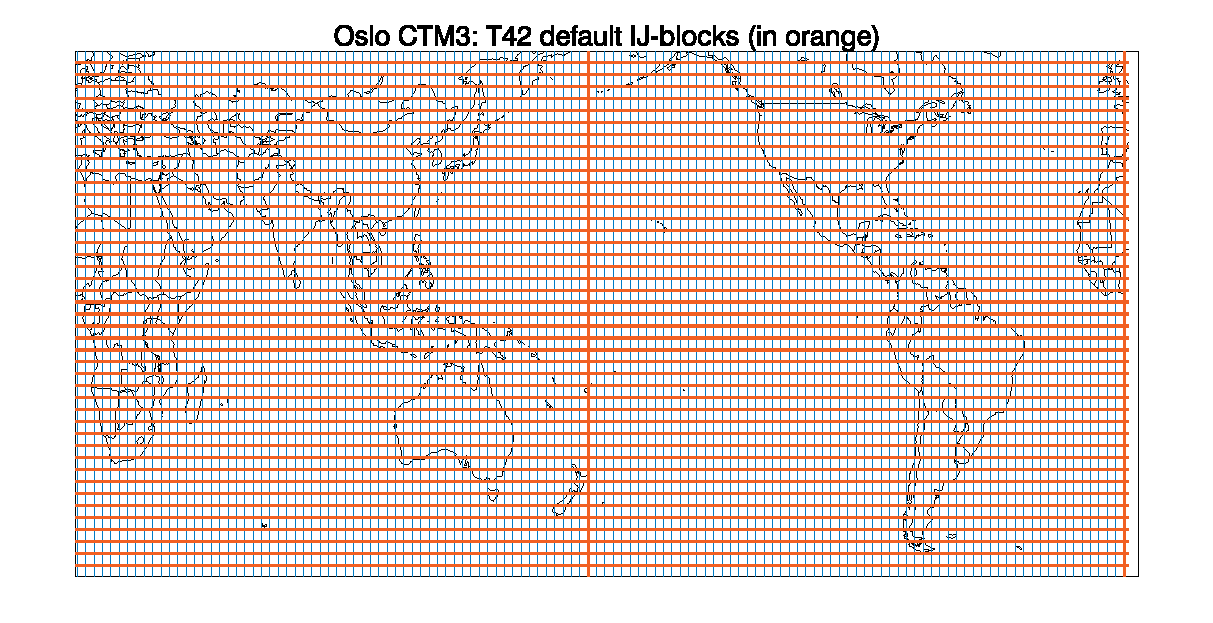
\includegraphics[width=0.94\linewidth]{figures/ctm3_mpblocks_t42_new}
  \caption{Default IJ-block structure for T42 horizontal resolution,
    where one block covers half the zonal direction
    and one latitude band.}
  \label{fig:mpblocks}
\end{figure}

Due to the IJ-block array structure, the loops will produce less
striding for long zonal blocks.
Depending on the resolution, the choice of \verb#MPIPAR# and
\verb#MPJPAR# must be tested to find which is faster.
%
For the older T42 and for newer 2x2 combined T159 horizontal
resolutions the default is
\verb#MPIPAR=2#\index{parallelisation!MPIPAR}\index{variables!MPIPAR} and
\verb#MPJPAR=JPAR#\index{parallelisation!MPJPAR}\index{variables!MPJPAR},
so that the IJ-blocks cover half of the zonal direction
(\verb#1:IPAR/2#), and one latitude band, as shown in
Figure~\ref{fig:mpblocks}.

It may, however, be that other configurations are better when
transporting few tracers.
For other resolutions there are other block sizes (defined
in {\it cmn\_size.F90}).
A~more thorough discussion on the IJ-block sizes is
included in Section~\ref{sxn:nrcpus}.

In \pmainf, the parallel index \verb#M# loops through the number of
IJ-blocks, and is passed on to subroutines where it is usually named
\verb#MP#. The global indices are accessible by using the variables
\verb#MPBLKIB#, \verb#MPBLKIE#, \verb#MPBLKJB# and \verb#MPBLKJE#
(all of size \verb#MPBLK#).
Their names \verb#MPBLKIB# and \verb#MPBLKIE# are somewhat
self-explaining; the first contains the zonal beginning point of all
IJ-blocks (i.e.~the global zonal indices), while the latter contains
the end points. Similarly, \verb#MPBLKJB# and \verb#MPBLKJE# are the
starting and end points in the meridional direction.
\index{parallelisation!access to global indices}
\index{parallelisation!MPBLKIB/MPBLKIE}\index{variables!MPBLKIB/MPBLKIE}
\index{parallelisation!MPBLKJB/MPBLKJE}\index{variables!MPBLKJB/MPBLKJE}
For a~given IJ-block (which have parallel index \verb#MP#), the first
global zonal index therefore is given by \verb#MPBLKIB(MP)# and ends
at \verb#MPBLKIE(MP)#, while the first global meridional index is
given by \verb#MPBLKJB(MP)# and ends at \verb#MPBLKJE(MP)#.

A~typical IJ-block loop is outlined in Table \ref{table:ijblock},
\begin{table}
  \caption{Looping through an IJ-block and accessing global and
  private variables, for component N.}
  \label{table:ijblock}
\begin{minipage}{\linewidth}
\strek
\vspace{-3mm}
\begin{verbatim}
  !// Loop over latitudes in IJ-block
  do J = MPBLKJB(MP),MPBLKJE(MP)
     !// IJ-block index JJ
     JJ   = J - MPBLKJB(MP) + 1

     !// Loop over longitudes
     do I = MPBLKIB(MP),MPBLKIE(MP)
        !// IJ-block index II
        II   = I - MPBLKIB(MP) + 1

        !// Corresponding local/global
        !// indices
        BTT(L,N,II,JJ) = STT(I,J,L,N)

     enddo
  enddo
\end{verbatim}
\vspace{-4mm}\strek
\end{minipage}
\end{table}
and you should understand how it works and why the reverse-ordered
B-arrays provide less striding\index{striding} (see
Section~\ref{sxn:programming_loops} for more on striding).
For global indices \verb#I,J# the local/private indices for IJ-block
number \verb#MP# are given by
\index{parallelisation!access to IJ-block indices}
\verb#II = I - MPBLKIB(MP) + 1#
and
\verb#JJ = J - MPBLKJB(MP) + 1#.

A~mapping from global indices \verb#I,J# to IJ-block number and local
indices can be found in the variable
\verb#all_mp_indices#\index{variables!all\_mp\_indices}\index{IJ-blocks!indices}\index{IJ-blocks!(I,J)~to~(II,JJ,MP)}\index{parallelisation!access to global indices}:\\
\verb#(II,JJ,MP) = all_mp_indices(1:3,I,J)#
%\verb#JJ = all_mp_indices(2,I,J)#\\
%\verb#MP = all_mp_indices(2,I,J)#\\



% Parallel layers
\subsubsection{Parallel layers}
\label{sxn:parallel:layer}\index{parallelisation!layers}
Horizontal advection, i.e.~transport between neighboring grid boxes,
have no need for information about boxes above or below. Hence, this
process carried out layer by layer, and a~processor calculates
transport of all tracers for one layer,
before being assigned (by OpenMP) a~new layer to transport.

It is also possible to do the transport component by component, so
that each processor work on each species, transporting them layer
by layer. Although this was done in \oldmodel, it is not done now. The
experience of the UCI group was that looping over layers is faster.
{\it Note also that studies with few tracers would limit effective
  use of the number of CPUs, if parallelisation is done over components.}


% OpenMP and advection
\subsubsection{OpenMP and advection}
\label{sxn:parallel:advection}\index{parallelisation!advection}
The important consequences of the advection treatment
(Section~\ref{sxn:parallel:ij} and \ref{sxn:parallel:layer}) is that
advection works both in IJ-block and layers and therefore need to go
in and out of IJ-blocks for each transported time step.
It means that increasing the number of operator split steps, also
increases the time spent shuffling data in and out of B-arrays;
transport may be better resolved, but it will be slightly more time
consuming.


% Writing parallelized code
\subsubsection{Writing parallelized code}
\label{sxn:parallel:writing_code}\index{parallelisation!writing parallelized code}
When you write a~new module, be sure to parallelize it! For most
processes or applications, it would be wise to use the IJ-block
structure, and therefore assign global arrays in reverse
order\index{reverse order}\index{indexing!reverse order}
(\verb#LPAR,IPAR,JPAR#), or even better by blocks
(\verb#LPAR,IDBLK,JDBLK,MPBLK#).

If your application works in the horizontal (this is less likely),
parallelisation should be layerwise, and global arrays should
{\it not} be reverse order but have the usual structure
(\verb#IPAR,JPAR,LPAR#).

Example: If you use 4~processes and your unparallelized application
uses 5\,seconds per time step (assuming one hour), it will contribute
with $\sim 12$\,hours of computing time when simulating one year.
Effectively parallelized, you could possibly divide this by the
numbers of processors, so that in using 4~CPUs you save 9~hours of
real computing time.

% Table: CPU timings
\begin{table}[!t]
  \caption{Computational efficiency when increasing the number of
    CPUs for T42L60 resolution. Timings are given in wall clock
    hours, for pure transport of 32 and 64 tracers, T42L60
    resolution, meteorological data for January 2005}
  \label{table:cpu}
\centering
  \begin{tabular}{c|c|c}
   \hline
      & T42L60\_32 & T42L60\_64 \\
   \hline
   4\,CPUs  & 1.72 & -- \\
   8\,CPUs  & 0.92 & 1.95 \\
   16\,CPUs & 0.57 & 1.08 \\
   32\,CPUs & 0.46 & 0.67 \\
   \hline
   8:4     & 0.53 & --   \\
   16:8    & 0.62 & 0.55 \\
   32:16   & 0.81 & 0.62 \\
   \hline
  \end{tabular}
\end{table}

% How many CPUs?
\subsubsection{How many CPUs and IJ-blocks?}
\label{sxn:nrcpus}\index{parallelisation!CPUs: how many to use?}\index{CPUs: how many to use?}
The more done in parallel, the more efficient and faster will the
program be. The \model\ is better parallelized than the \oldmodel,
however, there are a~few things you should be aware of when it comes
to the choice of CPU numbers and how it relates to the number of
IJ-blocks.

The number of IJ-blocks (set up in {\it cmn\_size.F90} should be close
to a~multiple of the number of CPUs, since the amount of work done in
a~column should be approximately the same for all columns.
However, this may not be true; the vertical transport (such ad
convection and advection) may have a~large impact on the time spent in
an IJ-block.

It is more difficult to do such a~choice for the horizontal transport,
since the amount of work done differ from layer to layer (shorter time
step for larger wind speeds).
However, the time spent in horizontal transport is relatively small,
so a~good choice for the number of CPUs will be a~multiple of
the number of IJ-blocks. As will be explained, the number of
IJ-blocks should be at least twice as large as the number of CPUs.

Since the time spent in each block may differ, it can be assumed that
OpenMP should use a~dynamic schedule. To make that efficient, the
number of blocks must be larger than the number of CPUs. But there is
also the possibility that too many CPUs may give larger
overhead. I~will discuss this further below.


% MP-blocks similar to number of CPUs
Timing tests of pure transport are included in Table~\ref{table:cpu},
showing that transporting 32~tracers on 8~CPUs and switching to
16~CPUs saves $\sim$40\,\% time, while switching from 16 to 32 only
saves~20\,\%.
However, transporting 64~tracers and switching from 16 to 32~CPUs also
saves about 40\,\%.
Hence, the number of IJ-blocks should be at least twice as large as
the number of CPUs.

The number of IJ-blocks and how they are defined also affect how
efficient the parallel code will be.
For the setting
\verb#MPIPAR=1#\index{parallelisation!MPIPAR}\index{variables!MPIPAR} and
\verb#MPJPAR=JPAR/2#\index{parallelisation!MPJPAR}\index{variables!MPJPAR},
each block will cover the whole zonal direction (\verb#1:IPAR#)
and two latitude bands.
Table~\ref{table:mpsize} shows a~few tests carried out for meteorologic
data of 1~January 2005, in T42N32L60 horizontal resolution, comparing CPU
timings for different IJ-block sizes.

% Table: CPU timings
\begin{table}[t!]
  \caption{Computational efficiency for different choices of IJ-block
    sizes, for 64 tracers in T42N32L60 resolution. Timings are
    for one day of transport (1~January 2005), given in
    wall clock seconds.}
  \label{table:mpsize}
\centering
  \begin{tabular}{l|c|c}
   \hline
   \multicolumn{3}{l}{Pure transport (average for 4~tests per case).} \\
   MPIPAR/MPJPAR   & 16\,CPU & 32\,CPU \\
   \hline
   1/16            & 120.8 & 112.0 \\
   1/32            & 122.0 & 71.4 \\
   2/16            & 119.6 & 72.5 \\
   1/64            & 116.7 & 69.6 \\
   2/32            & 115.0 & 69.3 \\
   2/64            & 110.8 & 68.0 \\
   \hline
   \multicolumn{3}{l}{Full chemistry (average for 3~tests per case).} \\
   MPIPAR/MPJPAR   & 16\,CPU & 32\,CPU \\
   \hline
   1/32            & 256.3 & 151.7 \\
   2/32            & 245.9 & 144.8 \\ 
   2/64            & 245.0 & 145.0 \\
   \hline
  \end{tabular}
\end{table}

Based on Table~\ref{table:cpu}, the number of blocks
should be at least twice the number of CPUs.
% Additional runs have been carried out to put further light on this.

It should be easily recognized that the number of IJ-blocks should be
at least as large as the number of CPUs, since most work is done in
the IJ-blocks used in parallelization.
16~IJ-blocks on 32~CPUs was only slightly faster than on 16~CPUs because
horizontal transport is parallelized over 60 model layers, where the
main improvement was.


Due to e.g.~read access limits, the timings varied slightly.
Therefore, each test was done 4~times, and the values
presented in Table~\ref{table:mpsize} are averages.
It seems that \verb#MPIPAR=2# and \verb#MPJPAR=JPAR# is
fastest for T42N32L60 transport, followed closely by
\verb#MPIPAR=2# and \verb#MPJPAR=JPAR/2#.

Adding chemistry makes the array sizes larger, and relatively more
work is done in the IJ-blocks.
One-day tests with full tropospheric and stratospheric chemistry show
that on 16~CPUs, \verb#MPIPAR=2# and \verb#MPJPAR=JPAR# saves about
10\,s per day, compared to \verb#MPIPAR=1# and \verb#MPJPAR=JPAR/2#.
Note that 10\,s per day amounts to $\sim$1\,hour of computing
time for one year.
For T42N32L60, the configuration \verb#MPIPAR=2# and \verb#MPJPAR=JPAR/2#
seems to be almost as fast as \verb#MPIPAR=2# and \verb#MPJPAR=JPAR#
on 16~CPUs, and slightly faster on 32~CPUs.
As the default IJ-block size for T42N32L60 we set
\verb#MPIPAR=2# and \verb#MPJPAR=JPAR#.

Using a~different date, where the meteorological conditions impose
a~shorter time step (10~Jan in this case), indicates that IJ-blocks
spanning more than 2~meridional boxes, e.g.~\verb#MPIPAR=2# and
\verb#MPJPAR=JPAR/4#, seem to make transport slower.

{\bf Higher resolutions}\\
For higher resolutions, the recommendation is a~bit more difficult.
Based on the transport tests, using
\verb#MPIPAR=1# and \verb#MPJPAR=JPAR#, was the fastest choice.
Adding chemistry and more species will increase the memory
use and potentially change this. In fact, tests done in 2018 suggested
\verb#MPIPAR=8# and \verb#MPJPAR=JPAR# as a~better option.


{\it Important}\\
However, the OpenMP scheduling has until 2018 been static (the default
scheduling). This means that every CPU know which IJ-block it will
calculate, and is likely not beneficial if the computing time differs
for each block (which it often does).
Therefore, the use of dynamic scheduling should be used. It adds some
overhead, but is generally faster unless the number of IJ-blocks is
very high compared to the number of CPUs used.
The difference between static and dynamic scheduling for 1280
IJ-blocks in T159N80L60 resolution was about 12\,\%.
Thus, the default value for T159N80L60 is set to
\verb#MPIPAR=8# and \verb#MPJPAR=JPAR#, i.e.~1280~IJ-blocks.

Also when combining 2x2 grid boxes, dynamic was clearly beneficial,
saving 10--20\,\% for \verb#MPIPAR=2# and \verb#MPJPAR=JPAR#.
It is not clear whether \verb#MPIPAR=2# is faster than \verb#MPIPAR=4#
for dynamic scheduling, but with static scheduling \verb#MPIPAR=4# is
worse.
As default, we keep the \verb#MPIPAR=2# and \verb#MPJPAR=JPAR# and use
dynamic scheduling for 2x2 combination of grid boxes.


The main lesson is: The number of IJ-blocks should be close to
a~multiple (2/4/8) of CPUs.
This should make sure that CPUs are not partially idle during
computation. E.g.~when using 80~IJ-blocks for T159N80L60 on 32~CPUs,
half of the CPUs will on average do 3~IJ-blocks, while the rest does~2.

As noted, vertical transport may change this slightly if time steps
differ greatly in different IJ-blocks. However, a~multiple of the
number of CPUs seems to be the best choice.

Keep in mind that machines sometimes are set up with hyperthreading,
telling you it has more CPUs than it actually has. The \model\ has
even shown slower performance when the number of CPUs requested is
higher than the number of physical CPUs (but within the threaded number).

In essence, when using other resolutions, you should check different
choices of IJ-blocks to find which is faster.

If you plan to use only one processor
(serial run)\index{parallelisation!serial run}\index{serial run},
you should still use several IJ-blocks. E.g.~one global IJ-block will
be large and not very efficient, since the whole global arrays will
have to be re-arranged.
Remember also that the efficiency is greatly reduced in a~serial run,
since the re-arranging of the structure is time consuming
{\it and carried out by one processor only}.



% Module based programming
\subsection{Module based programming}
\label{sxn:modulebased}\index{modules}
The model code has evolved from being partially Fortran90 to being
fully Fortran90 in 2015. Common blocks\index{modules!common block}
are no longer used, as they are marked obsolete by the Fortran company.

When you add new packages, you should program them as modules. It is
more flexible, and allows combining fixed format code with free format
code.
Another advantage is that you can define which parts of a~module you
want to access. You access the whole module with
\begin{verbatim}
  use <module>
\end{verbatim}\index{modules!use}
where \verb#<module># is the name of the module. This statement must
be placed before the \verb#implicit none# statement.

However, you get a~better code, which is easier to read and search or debug,
when you specify the variables and subroutines to use:
\begin{verbatim}
  use <module>, only: <variables, subroutines>
\end{verbatim}\index{modules!use}
where \verb#<variables, subroutines># is the list of needed variables
and/or subroutines, separated by commas.

If you include a~module A, which again includes a~module B, you have
indirectly access to all variables and routines in B. By using the
\verb#only# statement, this can be restricted.

For programming guidelines on how to make your subroutines optimal for
the \model, see Section~\ref{sxn:programming}.

%%%%%%%%%%%%%%%%%%%%%%%%%%%%%%%%%%%%%%%%%%%%%%%%%%%%%%%%%%%%%%%%%%%%%%
%%%%%%%%%%%%%%%%%%%%%%%%%%%%%%%%%%%%%%%%%%%%%%%%%%%%%%%%%%%%%%%%%%%%%%



%%%%%%%%%%%%%%%%%%%%%%%%%%%%%%%%%%%%%%%%%%%%%%%%%%%%%%%%%%%%%%%%%%%%%
% Programming guidelines -- #GUIDE
%%%%%%%%%%%%%%%%%%%%%%%%%%%%%%%%%%%%%%%%%%%%%%%%%%%%%%%%%%%%%%%%%%%%%%
\section{Programming guidelines}
\label{sxn:programming}
\index{programming guidelines}
Think structure! If you do not understand the structure of the model
(Section~\ref{sxn:structure}), you will probably end up with a~very
messy and inefficient code.

A~messy code may solve your problem, but should {\it never} be added
to the \model\ repository!


% Comment your code!
\subsection{Comment your code!}
\label{sxn:programming_comment}
\index{programming guidelines!comments}
Comment your code! Others should understand your code (and yourself
included after putting the code away for a~while). If you do
simplifications or approximations, include a~comment about why.

Comment so that a~newbeginner should understand quickly.
Never include comments that are not understandable, such as
``be careful''.

You should at least describe the following:
\begin{itemize2}
  \item Each module at the top of the file; its purpose and what it
    contains.
  \item Each subroutine, its purpose and variables, including the
    units of variables.
  \item All calculations. Include exact references if possible; if no
    reference is available, write why you do what you do.
    Write a~description that can be included in this manual at a~later
    stage.
\end{itemize2}


% Change existing code?
\subsection{Change existing code?}
\label{sxn:programming_changecode}
\index{programming guidelines!change existing code}
You should try to stay away from the existing core code except for
making master calls at the top level (\pmain) or in master
routines themselves.
If you think you need to do changes (especially big changes) in the
existing code\index{code!big changes in existing code?}, check with
the experienced programmers to find out if there may be better ways.


% Accessing cmn files in Fortran90 free format
\subsection{Accessing variables in Fortran90 free format}
\label{sxn:programming_f90}
\index{programming guidelines!accessing variables}
\index{free format}\index{free format!including cmn-files}
The Fortran90 free format is much easier to read than the fixed F77 style
format, and is more elegant. E.g., there is no limit on the number of
characters used on each line.

You can access variables from other modules in this way:
\begin{verbatim}
  use cmn_size, only: IPAR
\end{verbatim}


% Adding a new subroutine
\subsection{Adding a new subroutine}
\label{sxn:programming_newsubroutine}
\index{programming guidelines!adding a subroutine}
When you add a~new subroutine it should be included in
a~module\index{modules}\index{modules!use}\index{adding a subroutine}.
Global variables or parameters should also be specified in
this module, or possibly in common modules.

Still, there may be some very very few occasions, where it may be
necessary to add arrays to the core or the existing chemistry files,
but it should generally be avoided.

When adding a~new file, you need to include it in \makefile. How to do
this is explained in Appendix~\ref{app:makefile}.


% Adding new components
\subsection{Adding new components}
\label{sxn:programming_newcomps}
\index{programming guidelines!adding components}
When you add components, you need to make sure to change the number
of tracers in {\it cmn\_size.F90}\index{source code!core!cmn\_size.F90},
so that \makefile\ selects the right
numbers in compiling. Also make sure the tracer list\index{tracer list}
(\tracerlist) has the correct tracer numbers, names and molecular
masses.

The default length of tracer names (\verb#TMASS#\index{variables!TNAME}
and (\verb#XTMASS#\index{variables!XTNAME}) is 10, set by
\verb#TNAMELEN#\index{variables!TNAMELEN} in {\it cmn\_size.F90}.
If you need longer names, you have to modify \verb#TNAMELEN#.

Scavenging parameters are located in the file
\wetscavlist\ and \dryscavlist.\index{scavenging parameters}


% Efficient code
\subsection{Efficient code}
\label{sxn:programming_efficiency}
\index{programming guidelines!efficient code}
Think parallel! Whether you add processes or diagnostics, the work
should be done in parallel regions.

Diagnostics may be a~little tricky, since they often require access to
the global arrays. In this case, try to keep the arrays small, and do
calculations in the parallel regions. The goal
is to do as little as possible outside of the parallel regions (see
Section~\ref{sxn:parallel:writing_code}).

If you need to convert a~few tracers to another unit, you should only
convert the ones you need. See Section~\ref{sxn:programming_unit} for
more information on this.


% Unit conversion
\subsection{Unit conversion}
\label{sxn:programming_unit}
\index{programming guidelines!unit conversion}\index{unit conversion}
The tracer arrays are given in mass (kg) per grid box, and when you
need another unit you should create a~temporary array and convert it
on the fly, avoiding routines converting the whole tracer array.

All tracers are, however, converted before chemistry, and put into the
local array \verb#ZC_LOCAL#\index{variables!ZC\_LOCAL} (also
stratospheric components before doing tropospheric chemistry).
There is probably not much/anything to gain by only 
converting the tropospheric components for tropospheric chemistry and
vice versa for stratospheric chemistry, but it may be revised at
a~later stage.
%TOBEUPDATED when the trop/strat is called from the same master routine
However, only the tropospheric column is converted before tropospheric
chemistry (\verb#1:LMTROP(I,J)#), and only the stratospheric column 
before stratospheric chemistry (\verb#LMTROP(I,J)+1:LPAR#).

The conversion routines are located in
{\it utilities\_oslo.f90}\index{source code!oslo!utilities\_oslo.f90}.
Next follows descriptions of the conversions, you will probably need
them.


% Mass to concentration
\subsubsection{Mass to concentration}
\label{sxn:programming_mass2conc}
\index{programming guidelines!mass to concentration}\index{unit conversion!mass to concentration}
The unit of concentration is molec/cm$^3$. Conversion from mass
($m_t$) to concentration ($c_t$) involves the molecular mass (unit g/mol)
and volume (m$^3$). The conversion is done by
\begin{equation}
  c_t = m_t \frac{10^{-3}N_A}{M_t V}
  \label{mass2conc}
\end{equation}
where $N_A$ is the Avogadro's number ($6.022149\times 10^{23}$molec/mol),
$M_t$ is the molecular mass (or weight) of the tracer (g/mol), and $V$ is
the grid box volume (m$^3$). The factor $10^{-3}$ is a~combination of
converting $m_t$ from kg to~g and volume from m$^3$ to cm$^3$.

Converting the other way;
\begin{equation}
  m_t = c_t \frac{10^3 M_tV}{N_A}
  \label{conc2mass}
\end{equation}

$M_t$ is given in
\verb#TMASS#\index{variables!TMASS} for transported species and
\verb#XTMASS#\index{variables!XTMASS} for non-transported species.
Remember that they are indexed after transported and non-transported
numbers, not tracer IDs, so to get the correct molecular masses you
need the index arrays \verb#trsp_idx# and/or \verb#Xtrsp_idx#.


% Mass to mixing ratio
\subsubsection{Mass to mixing ratio}
\label{sxn:programming_mass2vmr}
\index{programming guidelines!mass to volume mixing ratio}\index{unit conversion!mass to volume mixing ratio}
By the term mixing ratio, the atmospheric chemistry community often mean
mole/number mixing ratio, which as I will show is the same as volume
mixing ratio for an ideal gas. In the aerosol field, however, mass mixing
ratio is more common.

Mass mixing ratio (mmr) unit is kg/kg, i.e.~mass of tracer ($m_t$) divided by
the mass of air ($m_a$). On the other hand, mole (or number) mixing ratio is
the number of tracer molecules ($n_t$) divided by molecules of air ($n_a$).
For an ideal gas, concentration is $c_t=n_tN_A/V$, and $c_a=n_aN_A/V$, so the
mixing ratio by volume is $c_t/c_a$.

For a~specific tracer, the relationship between mole ($n_t$) and mass
($m_t$) is:
\begin{equation}
  n_t = \frac{m_t}{M_t}
  \label{moles_from_mass}
\end{equation}

Thus, the conversion from mmr to vmr only involves
the tracer mass ($m_t$), air mass ($m_a$) and the molecular weights of
the tracer ($M_t$) and air ($M_a$):
\begin{equation}
  vmr = \frac{n_t}{n_a}
      = \frac{\frac{m_t}{M_t}}{\frac{m_a}{M_a}}
      = \frac{m_t}{m_a}\frac{M_a}{M_t}
  \label{mass2vmr}
\end{equation}

The number $M_a/M_t$ is available as
\verb#TMASSMIX2MOLMIX#\index{variables!TMASSMIX2MOLMIX}
for transported species and
\verb#XTMASSMIX2MOLMIX#\index{variables!XTMASSMIX2MOLMIX}
for non-transported species.

Note also that $m_t/m_a$ is the mass mixing ratio $mmr$.

Converting back to mass:
\begin{equation}
  m_t = vmr \times m_a \frac{M_t}{M_a}
  \label{mvr2mass}
\end{equation}
$M_t/M_a$ is available as the variable
\verb#TMOLMIX2MASSMIX#\index{variables!TMOLMIX2MASSMIX}
for transported species and
\verb#XTMOLMIX2MASSMIX#\index{variables!XTMOLMIX2MASSMIX}
for non-transported species, so to convert to mass mixing ratio you
multiply with \verb#TMOLMIX2MASSMIX# (or \verb#XTMOLMIX2MASSMIX#)
and then multiply with the air mass.


% Mass mixing ratio to volume mixing ratio
\subsubsection{vmr to mmr}
\label{sxn:programming_vmr2mmr}
\index{programming guidelines!vmr to mmr}\index{unit conversion!vmr to mmr}
The conversion from mass mixing ratio (mmr) to volume mixing ratio
(vmr) is very short and easy. Given tracer mass ($m_t$), tracer moles
($n_t$), air mass ($m_a$), air moles ($n_a$) and the molecular weights
of the tracer ($M_t$) and air ($M_a$):
\begin{eqnarray}
  mmr &=& \frac{m_t}{m_a} = \frac{n_t M_t}{n_a M_a}\nonumber\\
      &=& vmr \times \frac{M_t}{M_a}
  \label{vmr2mmr}
\end{eqnarray}
In other words: multiply volume mixing ratio by \verb#TMOLMIX2MASSMIX# (or
\verb#XTMOLMIX2MASSMIX# for non-transported tracers).


% Concentration to mixing ratio
\subsubsection{Concentration to mixing ratio}
\label{sxn:programming_conc2vmr}
\index{programming guidelines!concentration to volume mixing ratio}\index{unit conversion!concentration to volume mixing ratio}
You should not need this conversion, but I include it in case you
are interested. 
For an ideal gas the volume mixing ratio equals molecules of tracer
divided by molecules of air, i.e.~concentration of tracer divided by
concentration of air:
\begin{equation}
  vmr = \frac{c_t}{c_a}
  \label{conc2vmr}
\end{equation}
$c_a$ is the concentration of air -- i.e.~air density (molec/cm$^3$),
while $c_t$ is the tracer concentration. The air density is given as 
\verb#AIRMOLEC_IJ#\index{variables!AIRMOLEC\_IJ}\index{air density},
a~global field on IJ-block structure
(\verb#LPAR,IDBLK,JDBLK,MPBLK#) which is updated in the B-region at
each meteorological time step.

Equation (\ref{conc2vmr}) can also be derived from Equation
(\ref{conc2mass}) and (\ref{mass2vmr}):
\begin{eqnarray}
  vmr &=& c_t\frac{10^3 M_a V}{m_a N_A}\nonumber\\
      &=& \frac{c_t}{c_a}
\end{eqnarray}

Back to concentration:
\begin{eqnarray}
  c_t &=& vmr \frac{10^{-3}m_a N_A}{M_a V}\nonumber\\
      &=& vmr \times c_a
  \label{vmr2conc}
\end{eqnarray}



% Keep pmain.f90 clean
\subsection{Keep \pmain\ clean}
As noted in Section~\ref{sxn:structure_important}, you should not make
large changes in \pmainf.\index{pmain.f90!messing with pmain.f90}
It is supposed to be very short and easy to grasp. Only simple master
calls should be made from \pmain\ (which is possible; write master
routines!).


% Precision of numbers
\subsection{Precision of numbers}
\index{programming guidelines!use r8}\index{programming guidelines!double precision}
Variables should in general be defined as double precision, although
there are some exceptions. The precision parameters are set in
{\it cmn\_precision.f90}, and you should follow the existing
code. Do {\it not} use the old \texttt{real*8} method.

There are several definitions for precision:
%TOBEUPDATED rTnd should probably be split in rTnd2d and rTnd3d?
\begin{itemize2}
  \item \verb#r8#\index{r8}\index{precision!r8} is double precision.
  \item \verb#r4#\index{r4}\index{precision!r4} is single precision.
  \item \verb#rMom#\index{rMom}\index{precision!rMom} is the precision of
    the second order moments (standard is single precision).
  \item \verb#rAvg#\index{rAvg}\index{precision!rAvg} is the precision of
    average diagnostic arrays.
  \item \verb#rTnd#\index{rTnd}\index{precision!rTnd} is the precision of
    budget tendency arrays.
\end{itemize2}

Most computers work faster on double precision than on single
precision, so you should use double precision for floating point
numbers. Only for very large arrays a~gain can be achieved by using
single precision, since it may reduce the number of cache misses.
See Section~\ref{sxn:transport_som} for an example of this.


% Stay away from C-code
\subsection{Stay away from C-code}
From the start, the goal has been to keep the \model\ free of
C-code!\index{pmain.f90!C-code} Write dummy routines instead; if you
need an example, take a~look in the directory \oslopath\ vs
\oslopath{\it/DUMMIES} while you study the \makefile.

The only C-code allowed should be in the file {\it cmn\_size.F90}
(and of course the DUST code which I have not updated).


% Fortran loops
\subsection{Looping in Fortran}
\label{sxn:programming_loops}
\index{programming guidelines!looping in Fortran}\index{loops in Fortran}
Multidimensional arrays should be traversed in the natural ascending
storage order, which is column-major
\index{programming guidelines!column major order} order for
Fortran. This means that the leftmost index varies most rapidly
with a~stride of one.
For a~loop through the array \verb#ARR(IPAR,JPAR)#, the correct
traversing is shown in Table~\ref{table:flooping}.
\begin{table}
  \caption{Correct traversing of an array in Fortran.}
  \label{table:flooping}
\vspace{1mm}\begin{minipage}{\linewidth}
\strek\vspace{-3mm}
\begin{verbatim}
  do J=1,JPAR
    do I=1,IPAR
      ARR(I,J) = ...
    enddo
  enddo
\end{verbatim}
\vspace{-3mm}\strek
\end{minipage}
\end{table}

If you want to set the whole array
(e.g.~initialize\index{programming guidelines!initializing arrays} it),
use
\begin{verbatim}
  ARR(:,:) = 0.
\end{verbatim}
not just \verb#ARR = 0.#, which is possible: It makes the code easier
to read.
If you want to initialize only grid boxes I\,=\,10 to 20 and J\,=\,4 to
10, you can use \verb#ARR(10:20,4:10) = 0.#. The compiler will chose
the most efficient way to handle this.

If you are accustomed to C~programming, you should note that C~uses
row-major order\index{programming guidelines!row major order},
where the rightmost index varies most rapidly. If you put your 3D
or 4D array from C~coding into Fortran, it will be very ineffective,
striding\index{programming guidelines!striding}\index{striding} at
every step: If the array is of dimension
(\verb#IPAR#,\verb#JPAR#,\verb#LPAR#,\verb#NPAR#), and you loop
through it C-wise,
\begin{table}
  \caption{A very bad choice of C-looping in Fortran. {\it Do not do
      this in Fortran}.}
  \label{table:clooping}
\vspace{1mm}\begin{minipage}{\linewidth}
\strek\vspace{-3mm}
\begin{verbatim}
  do I=1,IPAR
    do J=1,JPAR
      do L=1,LPAR
        do N=1,NPAR
          ARR(I,J,L,N) = ...
        enddo
      enddo
    enddo
  enddo
\end{verbatim}
\vspace{-3mm}\strek
\end{minipage}
\end{table}
for every step of \verb#N# (from \verb#1# to \verb#NPAR#) it must jump
(stride) over \verb#IPAR#x\verb#JPAR#x\verb#LPAR# memory locations to
get to the next \verb#N# (see Table~\ref{table:clooping}).
{\bf You must not do this in Fortran!}

There are of course times when this needs to be violated, for example
when rearranging arrays into temporary arrays, with different
structures (see e.g.~Section~\ref{sxn:parallel}). In cases where the
temporary array is smaller, the largest arrays should be traversed in
column-major order, to keep the memory jumps as small as
possible.
Sometimes it may be difficult to decide which way to loop.


% Implicit none
\subsection{Implicit none}
\label{sxn:programming_implicitnone}
\index{programming guidelines!implicit none}\index{implicit none}
Always use implicit programming, starting each subroutine with
\verb#implicit none#. Explicit programming is very difficult to debug
if necessary, and should be avoided.

%%%%%%%%%%%%%%%%%%%%%%%%%%%%%%%%%%%%%%%%%%%%%%%%%%%%%%%%%%%%%%%%%%%%%%
%%%%%%%%%%%%%%%%%%%%%%%%%%%%%%%%%%%%%%%%%%%%%%%%%%%%%%%%%%%%%%%%%%%%%%



%%%%%%%%%%%%%%%%%%%%%%%%%%%%%%%%%%%%%%%%%%%%%%%%%%%%%%%%%%%%%%%%%%%%%%
% Transport -- #TRSP
%%%%%%%%%%%%%%%%%%%%%%%%%%%%%%%%%%%%%%%%%%%%%%%%%%%%%%%%%%%%%%%%%%%%%%
\section{Transport}
\label{sxn:transport}\index{transport}
Transport of atmospheric species is done by large scale advection,
convection and turbulent mixing. The latter is most important in the
boundary layer.
The basis for the \model\ transport is the Secondary Order Moments
scheme introduced by \citet{Prather1986}, which was later
re-structured and documented in \citet{PratherEA2008}.



% Secondary Order Moments
\subsection{Secondary Order Moments}\label{sxn:transport_som}
\index{transport schemes!secondary order moments}\index{secondary order moments}
In addition to transporting mean grid box values, the first and second
order moments are also transported. The first order moments carry 
information about the slope between grid boxes, while the second
order moments carry information about the curvature (the slope of the
slope).

The 3~first order moments are \verb#SUT#\index{variables!SUT},
\verb#SVT#\index{variables!SVT} and \verb#SWT#\index{variables!SWT}, and
the 6~second order moments are called \verb#SUU#\index{variables!SUU},
\verb#SVV#\index{variables!SVV}, \verb#SWW#\index{variables!SWW},
\verb#SUV#\index{variables!SUV}, \verb#SUW#\index{variables!SUW} and
\verb#SVW#)\index{variables!SVW}.
In result, there are 9~moments that need to be transported.

The moment array sizes are
(\verb#IPAR#,\verb#JPAR#,\verb#LPAR#,\verb#NPAR#), and their
units\index{secondary order moments!units} are
the same as for the mean grid value (i.e.~kg/grid box).
This may be somewhat counter-intuitive, but is explained
in \citet{Prather1986}.


The horizontal mass fluxes due to advection is stored in two arrays,
one for zonal divergence (\verb#ALFA#\index{variables!ALFA}) and one
for meridional (\verb#BETA#\index{variables!BETA}).
\begin{verbatim}
  ALFA(I,J,L) ==> [I,J,L] ==> ALFA(I+1,J,L)
  BETA(I,J,L) ==> [I,J,L] ==> BETA(I,J+1,L)
\end{verbatim}

Their units are~kg/s. See {\it p-dyn0.f}\index{source code!core!p-dyn0.f}
for more.


% CPU requirements
It is easy to see that transporting 10~variables per component will
require a~lot of CPU power, and that the memory requirements also are
relatively large\index{transport schemes!CPU requirements}.
The mass amounts carried by the moments are small compared to the
gridbox tracer average (\verb#STT#), and can therefore be stored in
single precision (defined by \verb#rMom#)\index{rMom}\index{precision!rMom}.
However, in the 1D~transport subroutine, everything is carried out in
double precision (\verb#r8#). Overall, this makes the code faster,
due to reduced code size and hence reduced cache misses.
It could be mentioned that conversion from single to double precision
takes some extra time, but the gain in a~reduced code size is much larger.
Comparison with double precision moments has been done, finding that
single precision do introduce some noise, but very small.


% Advection
\subsection{Advection}
\label{sxn:transport_adv}
\index{advection}
\index{transport schemes!advection}
Advection is carried out through the use of Secondary Order Moments
scheme, as described by \citet{PratherEA2008}. The transport papers
are available for free at his web
page\footnote{http://www.ess.uci.edu/$\sim$prather/}.

The global time step is based upon a~Lifshitz criterion, which in our
case is a~divergence criterion \citep{PratherEA2008}.
The transporting routine -- \verb#qvect3#\index{subroutines!qvect3} --
has an internal CFL criteria / time stepping\index{CFL criteria}.
The latter allows a~shorter time step at high latitudes where the grid
boxes are smaller compared to low latitudes.

Note that the Lifshitz criterion and internal CFL criterion may not
handle very rigorous deep convection well. Testing meteorological data
from an earth system model indicates this, giving negative air mass
after vertical transport if the number of advection steps is not
increased. I~have included a~crude fix for this in the routine
\verb#CFLADV#\index{subroutines!CFLADV} in {\it p-dyn0.f} -- if you
run into this problem, you may try that solution.


One of the major improvements from \oldmodel\ is that polar grid boxes
are no longer combined in transport (the so-called extended polar
zones).

There is, however, one important update from the 2008 description.
In \citet{SovdeEA2012}, the treatment of horizontal transport at the
polar caps was updated (see Section~\ref{sxn:transport_adv_hor}). 


% Horizontal advection
\subsubsection{Horizontal advection}
\label{sxn:transport_adv_hor}
\index{advection!horizontal}
The horizontal advection is carried out layer by layer, so that each
CPU works on a~whole layer. The routines are
\verb#DYN2UL#\index{subroutines!DYN2UL} and
\verb#DYN2VL#\index{subroutines!DYN2VL}, located in {\it p-dyn2.f}.

In \citet{PratherEA2008}, the polar cap treatment of horizontal
transport was to combine the polar boxes \verb#I# and \verb#I+IPAR/2#,
for meridional transport, while maintaining the gradients.
This did not work well, and was updated in 2011 to allow for a~more
accurate treatment, which are described in \citet{SovdeEA2012}.

For meridional transport, the two pie-shaped boxes on opposite sides
of the poles are no longer combined, and the V-flux across the pole is
zeroed and instead added to the U-flux (transport around the pole point).
To avoid short transport time steps due to small masses in the
polar-pie grid boxes, the default treatment in \model\ is to combine
boxes \verb#1:2# and \verb#JPAR-1:JPAR#, for
a~given \verb#I#, and maintain the moments.
An optional, more accurate treatment, is to skip the combining of
boxes, but that is more time consuming due to a~shorter global time
step required in transport.
The latter treatment improves cross-polar gradients, and should be
considered when studying e.g.~frozen-in anti-cyclones or O$_3$~holes.

To use this optional treatment involves using the files
{\it p-dyn0-v2.f}\index{source code!core!p-dyn0-v2.f} and 
{\it p-dyn2-v2.f}\index{source code!core!p-dyn2-v2.f} instead of the
standard {\it p-dyn0.f}\index{source code!core!p-dyn0.f} and 
{\it p-dyn2.f}\index{source code!core!p-dyn2.f}, and is explained in detail
in the horizontal transport section of \pmainf.


% Vertical advection
\subsubsection{Vertical advection}
\label{sxn:transport_adv_ver}
\index{advection!vertical}
The vertical advection is carried out column by column.
Large scale advection is computed from the continuity equation, as the global
field \verb#GAMA#\index{variables!GAMA}. In the IJ-blocks it is put into 
the field \verb#GAMAB#\index{variables!GAMAB}. Both advection and subsidence
due to convection (\verb#GAMACB#\index{variables!GAMACB}) are transported
together. I.e.~vertical advection must be calculated {\it after}
convection (Section~\ref{sxn:transport_conv}).

As the advection routine \verb#qvect3# needs the transport pipe to be
of {\it even number length}, care must be taken when using degraded
vertical resolution (L37/ or L57) (to get a~transport pipe of even
length).

There are two possible ways to create even length transport pipes, and
for very short arrays (e.g.~19 layers) this may also improve the speed
of the vertical advection:
\begin{itemize2}
  \item For each component, stack some columns on top of each other,
  to be transported as a~longer pipe.
  \item Stack several components from the same column in the longer
  pipe.
\end{itemize2}

The number of stacked columns or components is given by
\verb#IMDIV#\index{variables!IMDIV} in {\it cmn\_size.F90}, and is therefore
chosen automatically by \makefile.

Due to the model structure, stacking two components from the same
column works better than stacking two columns, since the minimum time
step needed in the pipe may differ in two columns:
Combining different columns means that the column with the shortest
time step forces the other columns to take a~shorter time step.
E.g.~convection may cause this, since it can vary much from column
to column.

Due to the structure of the B-arrays, this stacking of columns also
strides more than for tracer stacking, although that may not be a~big
problem for computers to handle.

For L60/L40 resolution, the fastest vertical advection is achieved by
no stacking at all. For special meteorological conditions using
\verb#IMDIV=1# halved the operator splitting time step compared to
\verb#IMDIV=4#.

Stacking components has, however, a~small disadvantage; If \verb#NPAR#
is not divisible with IMDIV, the remaining part of the transport pipe
will have to be filled with dummy tracers. The cost of this is small.
Choosing \verb#IMDIV=2# ensures the least number of dummies.

At some point the cost of creating a~long pipe will be larger than the
gain of using fewer pipes, reducing the efficiency of this method.
For L60 and L40 we use \verb#IMDIV=1#, while for L37 and L57 we use
a~pipe with 2~components, for both T42 and 1x1 horizontal resolution.


% Convection
\subsection{Convection}
\label{sxn:transport_conv}
\index{convection}
\index{transport schemes!convection}
Convective transport is calculated as a~separate process, and the
subsidence due to convection is calculated as a~mass flux
(\verb#GAMACB#\index{variables!GAMACB}). \verb#GAMACB# is treated
together with the large scale vertical advection
\verb#GAMA#\index{variables!GAMA} in the same transport routine
(\verb#DYN2W_OC#)\index{subroutines!DYN2W\_OC}.

The wet removal of gases due to convective rain is described in
Section~\ref{sxn:conv_scav}, whereas the transport is described here.

Convective transport is calculated using mass fluxes of updrafts and
downdrafts. The ECMWF IFS convective scheme is based on
\citet{Tiedtke1989}, so we use the same reference for the
\model\ convection.

Two important processes that occur in convection are entrainment and
detrainment. They can be separated into (1)~turbulent exchange through
cloud edges and (2)~organized exchanges. For updrafts the entrainment
can be noted
\begin{equation}
  E_{up} = E_{up}^{(1)} + E_{up}^{(2)}
\end{equation}
and detrainment
\begin{equation}
  D_{up} = D_{up}^{(1)} + D_{up}^{(2)}
\end{equation}


If you look at the IFS documentations, you will see that the
parameterisations change from cycle to cycle. In general  
\begin{equation}
  E_{up}^{(1)} = f D_{up}^{(1)}
\end{equation}
where $f$ may be unity or parameterized. $E_{up}^{(1)}$ is
proportional to the incoming mass flux and inverse proportional to the
cloud radii:
\begin{equation}
  E_{up}^{(1)} = f\frac{0.2}{R_{up}}\frac{M_{up}}{\overline{\rho}}
\end{equation}
where $\overline{\rho}$ is the air density. In this equation we locate
the fractional entrainment\index{convection!fractional entrainment}
(m$^{-1}$) as:
\begin{equation}
  \varepsilon_{up}^{(1)} = \frac{0.2}{R_{up}}
\end{equation}
See the IFS documentation for more on this and on equations for
$E_{up}^{(2)}$ and for detrainment.

{\it Important}\\
While the detrainment
rates\index{convection!detrainment rate}\index{detrainment!rate}
are given as [s$^{-1}$] in the IFS documentation, the meteorological
fields available (archived data) are mass flux per height,
i.e.~accumulated [kg/(m$^3$s)]\index{detrainment rate!units}\index{convection!detrainment rate!units}.

Available mass flux fields in the meteorological data are
\begin{itemize2}
  \item Updraft mass
    flux\index{convection!updraft mass flux}\index{updraft mass flux}
    (\verb#CWETE#\index{variables!CWETE})
  \item Downdraft mass
    flux\index{convection!downdraft mass flux}\index{downdraft mass flux}
    (\verb#CWETD#\index{variables!CWETD})
  \item Updraft detrainment rate
  \item Downdraft detrainment rate
\end{itemize2}


The detrainment rates are converted to entrainment mass
fluxes\index{entrainment!mass flux}
\verb#CENTU#\index{variables!CENTU} for
updrafts\index{entrainment!into updrafts} and
\verb#CENTD#\index{variables!CENTD} for
downdrafts\index{entrainment!into downdrafts}.
See Appendix~\ref{app:met_ctm_mflux} for some details on this.

For a~given grid box, the \model\ treatment of convection due to
updrafts consists of three parts, considering
\begin{itemize2}
  \item Mass flux in at bottom and out on top.
  \item Entrainment into updrafts from ambient air.
  \item Entrainment or detrainment to balance the net updraft mass
    fluxes and entrainment.
\end{itemize2}

It can be noted that the organized entrainment in the IFS model takes
place in the lowest part of the cloud, below the level of strongest
vertical ascent (explained in IFS documentation).
This information is lost for our use, but the balancing due to net
flux will retrieve some of the lost information.

In the convective routine the entrainment
\verb#CENTU#\index{variables!CENTU} is retrieved as
\verb#ENT_U#\index{variables!ENT\_U} and mass flux
\verb#CWETE#\index{variables!CWETE} as
\verb#FLUX_E#\index{variables!FLUX\_E}. For a~given layer \verb#L#,
with short notation, they are related as
\begin{equation}
  F_E(L) + E_U(L) - D_U(L) = F_E(L+1)
  \label{eq:fluxbalance}
\end{equation}
where $F_E$ is the mass flux from bottom of the given level, $E_U$ is
air entrained and $D_U$ is the detrained air at the same level
(positive if detrained).
In this way we allow detrainment to act as a~vent as the air is
rising, possibly increasing the mixing with the surrounding air in the
process (detrainment will leave polluted mass at lower levels,
transporting less to the plume top).

The detrainment $D_U(L)$ is positive when air leaves the convective plume
and is lost to the surroundings. From Eq.~(\ref{eq:fluxbalance}) we have:
\begin{equation}
  D_U(L) = - F_E(L+1) + ( F_E(L) + E_U(L) )
\end{equation}
However, it may be that this results in a~negative $D_U$, which means that
an additional amount of ambient air needs to be entrained from the
surroundings to balance the mass fluxes.

Downdrafts are explained in Appendix~\ref{app:met_ctm_mflux}.


% Boundary layer mixing
\subsection{Boundary layer mixing}
\label{sxn:transport_blmix}
\index{boundary layer mixing}
\index{transport schemes!boundary layer mixing}
The boundary layer mixing scheme is selected by the flag
\verb#NBLX#\index{variables!NBLX} in \maininput.
In the UCI code only the Prather scheme is available, but in the \model\ the
Holtslag scheme has been included from qcode~55.

The boundary layer is mixed each chemical time step, before chemistry.

It is important to notice that boundary layer height
(\verb#BLH#\index{variables!BLH}) is usually an instantaneous field, which
may be problematic during morning hours when photochemistry becomes effective
-- especially for thin boundary layer heights.

A~method for solving this is included, namely interpolating the \verb#BLH#
linearly in time between the current and the next meteorological time step
(\verb#BLH_CUR#\index{variables!BLH\_CUR} and
\verb#BLH_NEXT#\index{variables!BLH\_NEXT}, respectively).
The routine is called \verb#set_blh_ij#\index{subroutines!set\_blh\_ij},
and is called from \pmain, in the \verb#CCYC#-loop. To do this, each
IJ-block counts its elapsed seconds of the meteorological time step,
in the variable \verb#nmetTimeIntegrated#\index{variables!nmetTimeIntegrated}
defined in \pmain.

{\it Important}\index{boundary layer mixing!important}\\
This means that when using the time interpolation, \verb#BLH# should be
used with care in other routines.

Except from the boundary layer mixing routine, \verb#BLH# is put out in
several routines (vertical profiles and such), outside the IJ-block.
These routines put out values interpolated to each NOPS (if \verb#BLH_NEXT#
is available).


% Prather scheme
\subsubsection{NBLX=1: Prather scheme}\index{boundary layer mixing!Prather scheme}
The Prather bulk scheme uses e-folding time assuming full mixing in
3\,hours. The scheme is set up to be applied to collapsed bottom
layers (layer~1 consists of layer 1:3 and layer~2 of 4:5). The bulk
scheme should in principle be applicable to the full resolution, but
it may be too fast or slow.

It has been tested in the \ucimodel\ to do well compared with other
boundary layer schemes, although much simpler.
Some boundary layer parameters are still calculated.

The \model\ dry deposition used diffusitivities
(\verb#PBL_KEDDY#\index{PBL\_KEDDY}) for the lowermost model level,
which were only calculated in the Holtslag method.
A~separate calculation of \verb#PBL_KEDDY# has been included in the
Prather scheme.


% Holtslag
\subsubsection{NBLX=5: Holtslag}\index{boundary layer mixing!Holtslag scheme}
The \citet{HoltslagEA1990} k-profile scheme has been retrieved from
the previous version of the UCI model (qcode~55).
The boundary layer height needs to be doubled due to catch the whole
boundary layer. In L40, a~maximum of 9000\,m was used, but for L60
this had to be lowered to 8000\,m.
\begin{verbatim}
   ZBL = min(BLH(i,J)*2.d0,8000.d0)
\end{verbatim}

% Other
\subsubsection{Other schemes}
No other schemes are available, but qcode~55 also had code for
H\&R (NBLX=2), Louis (NBLX=3) and M-Y2.5 (NBLX=4).





%%%%%%%%%%%%%%%%%%%%%%%%%%%%%%%%%%%%%%%%%%%%%%%%%%%%%%%%%%%%%%%%%%%%%%
%%%%%%%%%%%%%%%%%%%%%%%%%%%%%%%%%%%%%%%%%%%%%%%%%%%%%%%%%%%%%%%%%%%%%%



%%%%%%%%%%%%%%%%%%%%%%%%%%%%%%%%%%%%%%%%%%%%%%%%%%%%%%%%%%%%%%%%%%%%%%
% Wet and dry scavenging -- #SCAV
%%%%%%%%%%%%%%%%%%%%%%%%%%%%%%%%%%%%%%%%%%%%%%%%%%%%%%%%%%%%%%%%%%%%%%
\section{Wet and dry scavenging}
\label{sxn:wetdrydep}
\index{scavenging}
Dry deposition is the process where gases are deposited on the ground,
i.e.~either through gravitational settling of by uptake processes in
the soil or in plants.
Thus it applies only to the lowermost model level.

Wet deposition, or scavenging, is when gases or aerosols are removed
by precipitation.

% Wet scavenging
%%%%%%%%%%%%%%%%%%%%%%%%%%%%%%%%%%%%%%%%%%%%%%%%%%%%%%%%%%%%%%%%%%%%%%
\subsection{Wet scavenging}
\label{sxn:wetscav}
\index{scavenging!wet scavenging}\index{wet scavenging}
Wet scavenging is usually divided into three types:
\begin{itemize2}
  \item {\it Rainout:} Used for aerosols when they act as
    cloud condensation nuclei (CCN) and fall out as rain.
  \item {\it Washout:} Gases/aerosols are deposited on rain
    drops. This is the usual mechanism for scavenging gases.
  \item {\it Sweepout:} When the rain droplets collect molecules or
    aerosols. Sometimes called {\it impact washout}.
\end{itemize2}
In \model\ we treat washout for both gases and aerosols, since
the meteorology (rain) is prescribed: We do not calculate the
precipitation from CCN. But the large scale scavenging scheme does
also calculate sweepout of species with mass limited washout
(i.e.~species which easily stick to water, such as HNO$_3$ and some
aerosols), called impact washout in the code.

It should be noted that the washout process is treated differently for
large scale and convective precipitation.

The wet scavenging parameters are found in the file \wetscavlist, as
listed in Tables~\ref{table:scavlist1}--\ref{table:scavlist3}.
It differs from the original UCI file, which is also available in
{\it scavng55.dat} for the interested reader.
In general, the scavenging follows Henry's law, so coefficients for
this are listed. How to specify more sophisticated effective
expressions is explained in Section~\ref{sxn:henryhardcode}.
The settings apply in general to the large scale wet scavenging, but
there are a~few options that only apply for convective scavenging.



% move parameter description here
The wet scavenging list contains parameters for convective scavenging
and large scale scavenging -- where some are specific for either convective
or large scale, but most apply for both. Here follows a list of the
parameters, which are also described at the end of the scavenging list.
\begin{itemize2}
  \item \verb#SOLU#\index{variables!SOLU}: Fraction of grid box
    available for wet scavenging. Applies for both convective and
    large scale scavenging. For convective scavenging, this must be
    accompanied by setting the flag \verb#CHN#\index{variables!CHN}
  \item \verb#CHN#\index{variables!CHN}: Defines treatment of
    convective scavenging, with the possibility to switch off liquid
    or ice large scale scavenging.
    Options are listed at the bottom of the scavenging file, and the
    most used flags are 0, 1 or 3. Large scale scavenging is treated
    unless stated otherwise:\\
    \begin{itemize2}
      \item[0] No convective scavenging.
      \item[1] Fraction dissolved is calculated from Henry
        coefficients, either using Henry's law or mass-limited. This
        fraction is multiplied with \verb#QFRAC#\index{variables!QFRAC}
        to get the fraction removed by scavenging
        (Section~\ref{sxn:conv_scav}--\ref{sxn:conv_scav_henrytheory}).
      \item[2] Not in use.
      \item[3] Assumes fully dissolved tracer, so that \verb#QFRAC#
        gives the fraction removed.
      \item[4] Removes fraction given by \verb#SOLU# and {\it not}
        \verb#QFRAC#.
        In other words: Everything is removed for \verb#SOLU=1#.
        Should be used with care!
      \item[5] Same as (3), but large scale scavenging is turned off.
      \item[6] Same as (3), but large scale scavenging on liquid is
        turned off. Large scale ice scavenging is included (if
        defined by \verb#ISCVFR#).
      \item[7] Convective removal only if minimum temperature in
        convective plume is lower than 258\,K.
        Large scale ice scavenging is included, but not liquid
        scavenging.
      \item[8] Convective removal only if minimum temperature in
        convective plume is lower than 258\,K and maximum temperature
        in plume is lower than 273\,K.
        Large scale ice scavenging is included, but not liquid
        scavenging.
    \end{itemize2}
  \item \verb#TCHENA#\index{variables!TCHENA}: First part of Henry
    expression, i.e.~Henry coefficient at 298\,K.
  \item \verb#TCHENB#\index{variables!TCHENB}: Exponential part of
    Henry expression, i.e. the temperature coefficient.
  \item \verb#TCKAQA#\index{variables!TCKAQA}: Flag for denoting
    that Henry expression should be modified by hard-coded settings.
    See \ref{sxn:henryhardcode} for more.
  \item \verb#TCKAQB#\index{variables!TCKAQB}: Zero is removal
    according to Henry expression, non-zero is mass (or kinetically)
    limited removal, which is used for highly soluble species.
  \item \verb#ISCVFR#\index{variables!ISCVFR}: Fraction of gridbox
    available for large-scale ice scavenging\index{ice scavenging}\index{scavenging!ice scavenging}.
  \item \verb#IT#\index{variables!IT}: Ice treatment when
    \verb#ISCVFR#>0.\\
    \begin{itemize2}
      \item[0] No scavenging below 258\,K.
      \item[1] For temperatures below 258\,K use \citet{KarcherVoigt2006}.
      \item[2] Use same treatment as for 258\,K\,--\,273\,K, i.e. with
        retention coefficient.
      \item[3] No removal for $T$<258\,K, but set retention
        coefficient to~1 instead of 0.5.
      \item[4] Standard treatment (Henry's law or kinetically limited)
        below 258\,K (as in option 2), but set retention
        coefficient to~1 instead of 0.5.
    \end{itemize2}
\end{itemize2}


% Large scale scavenging
%%%%%%%%%%%%%%%%%%%%%%%%%%%%%%%%%%%%%%%%
\subsubsection{Large scale scavenging}
\label{sxn:ls_scav}
\index{scavenging!large scale}
The large scale scavenging master routine located in
\verb#WASHOUT0#\index{subroutines!WASHOUT0}.
While the model in principle can use a~simplified scheme
(\verb#WASHOUT1#), it has been disabled for \model; we only use the
more sophisticated version by \citet{NeuPrather2012}
(\verb#WASHOUT2#), which scavenge separately by liquid and ice
precipitation.
It is still possible to choose the simple scheme by changing the
parameter \verb#NSCX#\index{variables!NSCX} in the input file
\maininput, but the data needed is not read into the model. If you
need that data, you can find it in {\it scavng55.dat}.

The \verb#WASHOUT2# is a~simple cloud model, dividing each grid box
layer in four parts:
\begin{itemize2}
  \item Cloud core, with rain coming in from above. Depending on how
    much rains out, rain may evaporate or be formed.
  \item Cloudy, with no rain coming in, but rain may form.
  \item Clear sky with rain from above.
  \item Clear sky with no rain.
\end{itemize2}
Fractional areas are calculated and may change e.g.~due to
evaporation. A~constant evaporation rate is used. More details are
explained by \citet{NeuPrather2012}.


For some species, such as HNO$_3$ and some aerosols, uptake on ice may be
important. Uptake on ice is controlled by a~non-zero ice scavenging fraction
\verb#ISCVFR#\index{variables!ISCVFR} in the scavenging list, denoting
how much of the grid box is available for ice scavenging.
For 258\,K\,<\,T\,<\,273\,K, the uptake is generally calculated using
Henry's law and the table-specified Henry's law coefficients, modified
by a~retention
coefficient\index{retention coefficient}\index{scavenging!retention coefficient}.
This is because Henry expressions are not given for
temperatures below 0$^{\circ}$C, and currently the retention
coefficient is set to~0.5 \citep{NeuPrather2012}.
Mass limited ice removal of species is calculated assuming a~Henry
coefficient of typically~10$^8$, which will yield the species completely
dissolved, even if the retention coefficient is 0.5.

Note that the retention coefficient can possibly be overwritten
by the \verb#IT# flags. In the future, it could be that the retention
coefficient could become part of the scavenging table.

Uptake of HNO$_3$ on ice can also occur below 258\,K, and follows
\citet{KarcherVoigt2006} when \verb#IT# is set to~1. Other options are
also available.



% Convective scavenging
%%%%%%%%%%%%%%%%%%%%%%%%%%%%%%%%%%%%%%%%%%%%%
\subsubsection{Convective scavenging}
\label{sxn:conv_scav}
\index{scavenging!convective}
Convective scavenging is adopted from the \oldmodel, and does not
separate between ice and liquid water; all is treated as rain.
It differs from the UCI method, which is rather crude.
The routines are called from \verb#CONVW_OC#\index{subroutines!CONVW\_OC}
and are located in
{\it cnv\_oslo.f90}\index{source code!oslo!cnv\_oslo.f90}.

If you need to do changes in that file, be certain that you understand
the units used; rain, liquid water and mass fluxes are kg/s.
Note that these values are accumulated in the meteorological data
files, and then converted. Entrainment into updrafts is originally not
flux, and is described in Section~\ref{sxn:transport_conv}.

Convection forms an elevator (or plume) transporting mass upwards.
To calculate the convective scavenging we need to know how much of
a~tracer that is solved in the liquid water of the elevator
(\verb#elev_mass_lw#)\index{variables!elev\_mass\_lw}, which is
described at the end of this section. The \verb#elev_mass_lw# also
covers the rain in the elevator.

The fraction of rain to liquid water in the elevator is called
\verb#QFRAC#\index{scavenging!QFRAC}\index{variables!QFRAC}.
Given an amount of tracer solved in the elevator liquid water,
the fraction \verb#QFRAC# is subject for removal.

Calculation is done using the mass fluxes from the meteorological data.
At the lowest level of entrainment, we entrain air and humidity from
the surroundings, to form the base of the elevator.
It is then lifted according to the mass fluxes, and assuming adiabatic
lifting, the elevator temperature cools and eventually water will
condense. The condensed water goes into \verb#elev_mass_lw#.
Entrainment or detrainment is then calculated, before we remove the
net rain out of the box. We do not consider net rain into the box to
increase \verb#elev_mass_lw#; with our simplified elevator, this
unfortunately not possible.

Eventually we reach the elevator top (determined by the mass fluxes)
and we have the following data for each level of the elevator:
Amount of liquid water, volume of elevator and volume fraction of
liquid water (droplets) in the elevator, which is called
\verb#LW_VOLCONC#\index{scavenging!LW\_VOLCONC}\index{variables!LW\_VOLCONC}
(e.g.~volume concentration). \verb#LW_VOLCONC# is used in calculating
the amount of tracer solved in the elevator. Some species are dissolved
completely (e.g.~HNO$_3$) and others are dissolved according to Henry's
law (Section~\ref{sxn:conv_scav_henrytheory}).

In the scavenging list, the parameters
\verb#SOLU#\index{scavenging!SOLU} and
\verb#CHN#\index{scavenging!CHN} 
defines whether or not each tracer is washed out by convection. These
data are stored in the model arrays
\verb#TCWETL(NPAR)#\index{variables!TCWETL} and
\verb#TCCNVHENRY(NPAR)#\index{variables!TCCNVHENRY}, respectively.
\verb#CHN# controls how to calculate the fraction of tracer
removed. Options are listed at the bottom of the scavenging file, and
also in the previous Section.

The use of Henry's law to find the fraction of tracer dissolved in the
elevator is described in the next Section.


% Theory on Henry's law
%%%%%%%%%%%%%%%%%%%%%%%%%%%%%%%%%%%%%%%%%%%%%
\subsubsection{Theory on Henry's law}
\label{sxn:conv_scav_henrytheory}
Looking at the convective scavenging code, you find a~fraction
of dissolved tracer on the form
\begin{equation}
  f_{dissolved} = \frac{H_H LW_{volconc}}{H_H LW_{volconc} + 1}\label{eq:fdis}
\end{equation}
A~similar expression can be found in the large scale scavenging
routine (subroutine HENRYS\index{subroutines!HENRYS}, although it is
different below 273\,K).
% Should write more on that...
I will explain the background of this equation here.

First of all, there are several data on Henry coefficients; usually
they are given at 298\,K, together with a~temperature coefficient.
Another possibility, as in \citet{jpl10-06}, coefficients are given
for the expression:
\begin{equation}
  \ln H(T) = A + \frac{B}{T} + C\,\ln T
\end{equation}
Coefficient $C$ is rarely used, and while $B$ is used by the \model, I
stress that this $A$-coefficient differs from the model definition:
\model\ applies the well used van't Hoff's temperature
extrapolation from 298\,K. This extrapolation assumes that Henry's law
varies as
\begin{equation}
  \frac{d\,\ln H}{d\,T} = \frac{\Delta H_{sol}}{RT^2}
\end{equation}
where $\Delta H_{sol}$ is the solution enthalpy. $\Delta H_{sol}$ is
assumed constant (a~fairly good approximation), so that the expression
can be re-arranged and integrated between temperatures $T_1$ and $T_2$:
\begin{equation}
  H(T_2) = H(T_1)\,\exp\left[\frac{\Delta H_{sol}}{R}
           \left(\frac{1}{T_1}-\frac{1}{T_2}\right)\right]
\end{equation}
The temperature dependence
\begin{equation}
  \frac{\Delta H_{sol}}{R} = - \frac{d\,\ln H}{d(\frac{1}{T})}
\end{equation}
is the $B$ coefficient given e.g.~by \citet{jpl10-06} and also
used in the \model. Hence, using $T_2=298$\,K, the model finds the
Henry expression at any temperature:
\begin{equation}
  H(T) = H(298\,\mathrm{K})\,\exp\left[B
           \left(\frac{1}{T}-\frac{1}{298\,\mathrm{K}}\right)\right]
\end{equation}
This means that the $A$-coefficient used in the model (in scavenging
table), is in fact $H(298\,\mathrm{K})$.

The following explanation applies to the convective scavenging, 
where $LW_{volconc}$ is calculated. In the routine for large scale
scavenging, $LW_{volconc}$ is not explicitly calculated, which is why
Eq.~(\ref{eq:fdis}) differs slightly in that routine. However, the
basics behind it is the same.

{\it Important notice}\\
When Eq.~(\ref{eq:fdis}) is used and $LW_{volconc}$ is calculated, as
in the convective routine, $H(T)$ has to be modified to get the
correct units, i.e.~we have to multiply it by $R\,T$, where
$R=0.08206$\,atm\,L\,mol$^{-1}$\,K$^{-1}$.

{\bf Deriving Eq.~(\ref{eq:fdis})}\\
Henry's law coefficient for any gas is defined as
\begin{equation}
  P_{gas} = k_H  X
\end{equation}
where $P_{gas}$ is the partial pressure of the gas above the solution,
and $X$ is the molar fraction of the dissolved gas in the solution;
\begin{equation}
  X = \frac{n_{aq}}{n_{aq} + n_{solvent}}
\end{equation}
where $n_{aq}$ is the number of moles solved, and $n_{solvent}$ is
the number of moles of the solvent (i.e. water in our case).

Assuming ideal solution, we can change to concentration by dividing
by volume of the solution, and get:
\begin{equation}
  X = \frac{C_{aq}}{C_{aq} + C_{solvent}}\nonumber
\end{equation}
As long as Henry's law applies, i.e. the species is {\it not} highly
soluble, we always have $C_{aq} \ll C_{solvent}$, and can approximate
to:
\begin{equation}
  X = \frac{C_{aq}}{C_{solvent}}
\end{equation}

Since the concentration of the solvent (water) is approximately constant,
we arrive at the other common form of Henry's law:
\begin{equation}
  P_{gas}= k  C_{aq}
\end{equation}

Units for $k$: [atm L(solvent)/mol], and for $P_{gas}$: [atm].

If $k$ is high, it means the component prefers thermodynamically
to be in gas phase.

We are interested in calculating $C_{aq}$ from $P_{gas}$, so we
introduce
\begin{equation}
  H_{STAR} = 1/k
\end{equation}
with units [mol/(atm L(solvent))], so that
\begin{equation}
  C_{aq} = H_{STAR}  P_{gas}
\end{equation}

If we want to apply the calculations to molar concentration (mol/L),
we have to change some units:
\begin{equation}
  P_{gas} = C_g  R  T
\end{equation}
given correct units of R, i.e. [atm L /(mol K):
\begin{itemize2}
  \item J = kgm$^2$/s$^2$ = Pa m$^3$
  \item R = 8.31451J/(mol K) / 101325Pa/atm \\ x 1000 L/m$^3$
          = 0.0820578 atm L/(mol K)
\end{itemize2}
Henry's law therefore implies that the concentration in the solution
is proportional to the atmospheric concentration: 
\begin{equation}
  C_{aq} = H_{STAR}  R  T  C_g = H_H  C_g\label{eq:henry_caq}
\end{equation}
where $H_H$ has the units [mol/L(solvent) / (mol/L(air))].

We want the mass fraction of the dissolved gas, which equals the
molar fraction $f_{dissolved}$.
\begin{equation}
  f_{dissolved} = \frac{n_{aq}}{n_{aq} + n_g}
\end{equation}

The volumes have units [m$^3$], while the number concentration of
tracer in air, $C_g$, has units [mol/L(air)]. Hence, we get the moles
of tracer in gas phase:
\begin{equation}
  n_g  = C_g  V_{elevator\_air}
     \frac{10^3\textrm{L(air)}}{\textrm{m}^3\textrm{(air)}}
\end{equation}

$C_{aq}$ has units [mol/L(solvent)], and the number of moles in
the solution is
\begin{eqnarray}
  n_{aq} &=& C_{aq}  V_{elevator\_solvent}\label{eq:n_aq}\\
         &&  \cdot10^3\textrm{L(solvent)/m}^3\textrm{(solvent)}\nonumber
\end{eqnarray}

As already explained, the solvent is liquid water.
The volume of the solvent is given by the liquid water content, and is
calculated in elevator fractions as volume concentration, i.e.~volume
of liquid water in elevator to total elevator volume. As can be found
in the source code comments, the volume of liquid water is
\begin{equation}
  V_{elevator\_solvent} = \frac{\textrm{mass of liquid water}}{\rho}
\end{equation}
where $\rho$ is the density of water (which is $10^3$\,kg/m$^3$).
The liquid water volume concentration is then
\begin{equation}
  LW_{volconc} = \frac{V_{elevator\_solvent}}{V_{elevator\_air}}
  \label{eq:lwvolconc}
\end{equation}

Using Equation~(\ref{eq:n_aq}) and~(\ref{eq:lwvolconc}), the moles of
gas dissolved in water is
\begin{eqnarray}
  n_{aq} &=& C_{aq} LW_{volconc} V_{elevator\_air}\\
         &&    \cdot10^3\textrm{L(solvent)/m}^3\textrm{(solvent)}
\end{eqnarray}

The mass fraction dissolved in the droplets (mass fraction equals mole
fraction in this case), which is subject to washout, is therefore
\begin{eqnarray}
  f_{dissolved} &=& \frac{n_{aq}}{n_{aq} + n_g}\nonumber\\
          &=& \frac{C_{aq} LW_{volconc}}{C_{aq} LW_{volconc} + C_g}
\end{eqnarray}
and by Equation~(\ref{eq:henry_caq}) we get
\begin{equation}
  f_{dissolved} = \frac{H_H LW_{volconc}}{H_H LW_{volconc} + 1}
  \label{eq:fdissolved}
\end{equation}
In the \model\ code this fraction is called
\verb#DISSOLVEDFRAC#\index{variables!DISSOLVEDFRAC}.

When the retention coefficient\index{retention coefficient}\index{scavenging!retention coefficient}
is used in large scale scavenging, it is multiplied by $H_H$ in
Equation~(\ref{eq:fdissolved}).


% Hardcoding Henry coefficients
%%%%%%%%%%%%%%%%%%%%%%%%%%%%%%%%%%%%%%%%%%%%%
\subsubsection{Hard-coded Henry coefficients}
\label{sxn:henryhardcode}
Some tracers have empirical Henry constants, which need to be
hard-coded. This is specified by a~non-zero
\verb#TCKAQA#\index{variables!TCKAQA} in
the scavenging list \wetscavlist.

The hard coding is done in the routine
\verb#getHstar#\index{subroutines!getHstar} in
{\it scavenging\_largescale\_uci.f90}\index{source code!oslo!scavenging\_largescale\_uci.f90}, called by either the large scale scavenging routine or
the convective scavenging routine.



% Dry deposition
%%%%%%%%%%%%%%%%%%%%%%%%%%%%%%%%%%%%%%%%%%%%%%%%%%%%%%%%%%%%%%%%%%%%%%
\subsection{Dry deposition}
\label{sxn:drydep}
\index{dry deposition}
Deposition velocities are stored in
\verb#VDEP#\index{dry deposition!VDEP}\index{variables!VDEP}
of size (\verb#NPAR#,\verb#IPAR#,\verb#JPAR#), thus allowing for
possible deposition of any transported tracer.

% Units
\verb#VDEP#\index{variables!VDEP} is given in units [m/s], and is set
in subroutine \verb#setdrydep#\index{subroutines!setdrydep} in
the file
{\it drydeposition\_oslo.f90}\index{source code!oslo!drydeposition\_oslo.f90},
which is called from \pmain.

{\bf Important 1}\\
When these deposition velocities are to be used in QSSA, they have to
be divided by the height of the lowermost layer, to get the
unit~[s$^{-1}$]. This is carried out e.g.~before chemistry
(\verb#MASTER_OSLO#) and in subroutine \verb#bcoc_master#.


{\bf Important 2}\\
Inspired by CTM2-tests done by others, I started in 2013--2014 to make
an update of the dry deposition scheme. However, I never got to finish
it. Early 2018, I got a small opportunity to look at it again, and
made some small changes, so the new scheme may be tested properly.

The \oldmodel\ parameterisation, which is the standard scheme,
is explained very briefly in Section~\ref{sxn:drydeptech_history},
while the new scheme is described in
Section~\ref{sxn:drydeptech_new}--\ref{sxn:drydeptech}.



% Technical: Historical note
\subsubsection{Historical note}
\label{sxn:drydeptech_history}
\index{dry deposition!technical description: historical note}
In the \model\ \citep{SovdeEA2012} and its predecessor Oslo~CTM2
dry deposition has been parameterised based on \citet{Wesely1989},
not by calculating the deposition velocities from equations, but
rather by using seasonal day and night averaged deposition velocities
for different land use types.
However, some velocities seem to rather come from \citet{Hough1991}.

Using 5~land-use types (water, forest, grass, tundra/desert and
ice/snow) in each gridbox, a~mean velocity was then defined.
Day and night was defined by using the solar zenith angle (subroutine
\verb#SOLARZ#), giving day if less than 90$^{\circ}$.
Winter was defined as temperatures below 273.15\,K for grid boxes
containing land masses. Ocean gridboxes containing sea ice use
ice/snow values, but a~distinction on season was not necessary because
the summer and winter values are equal.
However, snow cover was taken into account, reducing uptake when snow
thickness was about 1\,m (10\,cm water equivalents) in forest and
10\,cm (1\,cm water equivalents) on grass/tundra.

The old UCI read-in is disabled, but a~short note about it is given in
Section~\ref{sxn:drydep_uci}.


% Technical: Dry deposition update
\subsubsection{The new dry deposition scheme}
\label{sxn:drydeptech_new}
The dry deposition parameterisation is in the process of being
updated to follow the method of the EMEP model \citep{SimpsonEA2012}.
It is a~more physical approach and is described in detail in
Section~\ref{sxn:drydeptech}.

The EMEP method is used for the gaseous species
O$_3$, H$_2$O$_2$, NO$_2$, PAN, SO$_2$, NH$_3$, HCHO, CH$_3$CHO.
CO has a~very small uptake and is not included in the EMEP
treatment, so we keep the old \oldmodel\ parameterisation.

Some of the aerosol deposition rates follow the EMEP aerosol
parameterisation, namely BC/OC aerosols, sulphur aerosols
(SO$_4$ and MSA), and secondary organic aerosols (SOA).
Other aerosol modules have their own parameterisations which are
described in their own sections of this manual.


My first tests showed that the new parameterisation improved
the ability to reproduce measured surface O$_3$.
Generally, the largest impacts can be found for 
O$_3$, HNO$_3$, SO$_2$ and NH$_3$, but also for SO$_4$ due to changes
in SO$_2$.

However, the 2018 version of the new scheme uses a~more physically
correct value of the stomatal conductance, calculated by the
MEGANv2.10 module. It is also possible to use a~climatology of
stomatal conductance, but I would not recommend it.

%TOBEUPDATED
Tropospheric burden of O$_3$ and HNO$_3$ increased by~5--8\,\% and
5--10\,\%, respectively. A~$\sim$20\,\% decrease was found for
tropospheric SO$_2$ and SO$_4$, while NH$_3$ tropospheric burden
decreased by 20--30\,\%.
The other species do not change much (0--3\,\%). Interestingly,
NO$_2$ decreases slightly during winter but increases more during
summer, showing that secondary effects coming from chemistry are also
important.




% Technical: Dry deposition
%%%%%%%%%%%%%%%%%%%%%%%%%%%%
\subsubsection{Technical description: gaseous species}
\label{sxn:drydeptech}
\index{dry deposition!technical description: gaseous species}
Typically, deposition uptake follows an~electric
circuit analogy, where the deposition velocity $v_d^i$ for species $i$
is
\begin{equation}
  v_d^i = \frac{1}{R_a + R_b^i + R_c^i}\label{eq:vdi}
\end{equation}
where $R_a$ is the aerodynamical resistance between the surface and
the top of the vegetation canopy (i.e.~the altitude $z_0$, called
roughness length), $R_b^i$~is the quasi-laminar layer resistance to
the gas and $R_c^i$~is the canopy resistance (often called surface
resistance and sometimes denoted~$r_s^i$).

$R_a$ is the same for all gases, depending only on the surface/air
properties. $R_b^i$ and $R_c^i$~are different for all gases, and the
latter also vary from vegetation type to vegetation type.

The inverse of a~resistance is called conductance, which is
denoted~$G$:
\begin{equation}
  G = \frac{1}{R}
\end{equation}
Conductance is in essence the same as velocity. This is important to
keep in mind when calculating an average deposition value in
a~gridbox.

If Eq.~(\ref{eq:vdi}) is the gridbox average, then the $R$s are grid
box effective averages. This must be kept in mind when calculating grid box
averages of $R_c^i$, which depend on land-use types; then we need to
calculate resistances for all vegetation types and do a~proper
weighting to get the gridbox average.

To do this weighting we recognise that a~molecule can only choose
one land type; it will not take the least resistance of several
land-use types.

As an example, assume we have 2~land-use types with gridbox fractions
being 50\,\% each, with resistances
$R_1=1$\,s/m and $R_2=10000$\,s/m.
A~molecule is located above one of these surfaces and cannot choose
where to go. This means that several land-use types,
e.g.~forest and grass, cannot occupy the same area when the area is
infinitesimally small (approaches zero).

Each of these two areas would have their respective velocities
$v_i=1/R_i$, i.e.~$v_1=1$\,m/s and $v_2=10^{-4}$\,m/s. The small
velocity will remove little, but if the big velocity would remove
almost everything, it would in this case remove half of the species in
the whole gridbox.

Then it is easy to see that the gridbox effective average $R$ is found
by
\begin{equation}
  \frac{1}{R} = f_1 \cdot \frac{1}{R_1} + f_2 \cdot\frac{1}{R_2}
\end{equation}
which is actually the average conductance
\begin{equation}
  G = f_1\cdot G_1 + f_2 \cdot G_2
\end{equation}

giving $v \approx 0.5$\,m/s. If $v=1$\,m/s would remove all in the gridbox, 
$v=0.5$\,m/s removes half, as expected.

Had we used ($f_1*R_1+f_2*R_2$) as the average resistance, the
velocity would be $0.0002$\,m/s, which is clearly not what we want.

Hence, it is the velocities (or conductances) which have to be
weighted according to land-use fractions, to get a~gridbox mean
velocity.


% New dry deposition scheme
The new dry deposition scheme calculates $R_a$, $R_b^i$ and $R_c^i$
following \citet{SimpsonEA2012}, which will be referred to as
EMEP2012. Main gases included are O$_3$, SO$_2$, NH$_3$, NO$_2$,
H$_2$O$_2$ and HNO$_3$, but in addition I have included NO, HCHO and
CH$_3$CHO which to some extent are also subject to dry deposition.

As already noted, dry deposition of CO is still treated with the old
scheme. This is because it is not available through EMEP2012. In
general, CO dry deposition is so small that models tend to exclude
it. It is set to 0.03\,cm/s over vegetated areas
\citet{ConradSeiler1985}, and it is reduced when there is snow.

Aerosols are not part of the new update and follows the old deposition
treatment, using fixed deposition velocities or calculated separately
as in the sea salt or mineral dust modules.


{\bf Important}\\
To use this treatment, both the nitrate and sulphur modules should be
included. They are needed for calculation of SO$_2$ deposition which
is again needed to calculate dry deposition velocities for other
gases.
Note that \citet{SovdeEA2012} concluded that these modules should be
included anyway; doing so does not increase computing time by much.
Still, if sulphur and nitrate are not included, a~monthly model
climatology of the parameters $a_{sn}$ and $a_{sn}^{24h}$ is needed.

However, this climatology has not yet been produced, so if you try to
run the model without sulphur and nitrate modules, the program will
stop.


% Aerodynamical resistance (Ra)
{\bf Aerodynamical resistance R$_a$}\index{dry deposition!aerodynamical resistance (Ra)}\\
The aerodynamical resistance ($R_a$) in EMEP2012 is not well defined
in \citet{SimpsonEA2012}. They first assess friction velocity $u_*$ by
using stability functions (Eq.~(52) in EMEP2012):
\begin{equation}
  u_* = \frac{V_H(z)\,k}{
    \ln\left(\frac{z-d}{z_0}\right)
     - \Psi_m\left(\frac{z-d}{z_0}\right)
     - \Psi_m\left(\frac{z_0}{L}\right)}
\end{equation}
Here, $V_H(z)$ is the wind speed at their reference height $z$ and
$\Psi_m$ represents the integrated stability equations for momentum,
$d$ is a~constant (typically 0.7\,m), and $L$ is the Obukhov length.
However, they do not list the equation for $R_a$.

A~somewhat similar expression is found for $R_a$ in the earlier EMEP
version \citep[EMEP2003,][]{SimpsonEA2003},
namely
\begin{equation}
  R_a = \frac{1}{k\,u_*}\left[
    \ln\left(\frac{z-d}{z_0}\right)
     - \Psi_h\left(\frac{z-d}{z_0}\right)
     - \Psi_h\left(\frac{z_0}{L}\right) \right]\label{eq:ra1}
\end{equation}

However, for certain values of $z$, $z_0$ and $L$, Eq.~(\ref{eq:ra1})
can produce a~negative $R_a$, which is wrong. This also applies to the
$u_*$ calculation of EMEP2012.

Therefore we use a~different approach in \model, namely the method
of \citet{Monteith1973}. Sensible heat flux ($SHF$) between surface
and air is given by
\begin{equation}
  SHF = \rho c_p \frac{T_0-T_z}{R_{a,H}}\label{eq:ra2}
\end{equation}
where $\rho$ is air density, $c_p$ the specific heat at constant
pressure, $T_0$ is the surface temperature, $T_z$ is the temperature
at reference height $z$, and the aerodynamic resistance $R_{a,H}$ is
the diffusion resistance to sensible heat transfer between surface and
the reference height~$z$.
In \model\ it is assumed that $R_a=R_{a,H}$.

Sensible heat flux can also be written
\begin{equation}
  SHF = -\rho c_p K_H\frac{\partial T}{\partial z}\label{eq:monSHF}
\end{equation}
and momentum flux using the wind $u$ profile
\begin{equation}
  MF = -\rho u_*^2 = \rho K_M\frac{\partial u}{\partial z}\label{eq:monMF}
\end{equation}
where $K_H$ and $K_M$ are the respective eddy diffusitivities.
When $K_M=K_H$, Eq.~(\ref{eq:monSHF}) and (\ref{eq:monMF}) gives
\begin{equation}
  SHF = - \rho c_p \frac{\partial T}{\partial u} u_*^2
\end{equation}
which in finite differences between surface and reference height $z$
can be written
\begin{equation}
  SHF = \rho c_p (T_0-T_z) \frac{u_*^2}{u_z}
\end{equation}
where $T_z$ and $u_z$ are temperature and wind speed at height~$z$.
From Eq.~(\ref{eq:ra2}) we get the \citet{Monteith1973} equation for
$R_{a,H}$:
\begin{equation}
  R_{a,H} = \frac{u_z}{u_*^2}
\end{equation}
This is what we use for $R_a$ in \model, and as reference height we
use the midpoint of the surface model level. This level is about 16\,m
thick, so the reference height is about~8\,m.
This is possible because both $u_z$ and $u_*$ are available from the
meteorological data.


% Quasi-laminar layer resistance (Rb)
{\bf Quasi-laminar layer resistance R$_b$}\index{dry deposition!quasi-laminar layer resistance (Rb)}\\
$R_b^i$ is species specific, and is defined differently over land and
ocean. When a~gridbox contain both land and ocean, a~weighted mean
$R_b^i$ is calculated using the respective land and ocean
conductances.

Over land we use
\begin{equation}
  R_b^i = \frac{2}{k\,u_*} \left(\frac{Sc_i}{Pr}\right)^{2/3}
\end{equation}
where $Pr$ is the Prandtl number (0.72) and $Sc_i$ is the Schmidt
number for gas $i$, defined as:
\begin{equation}
  Sc_i = \frac{\nu}{D_i}
\end{equation}
Here $\nu$ is the kinetic viscosity of air and $D_i$ is the molecular
diffusivity for gas $i$. If you look at the code, you will see that
the $Sc_{H_2O}=0.6$ as well as $D_{H_2O}=0.21\cdot 10^{-4}$ are
defined, and that $Sc_i$ is found from
\begin{equation}
  Sc_i = Sc_{H_2O}\frac{D_{H_2O}}{D_i}
\end{equation}
where $D_{H_2O}/D_i$ is listed in Table~\ref{table:wesely}.

Over sea we use
\begin{equation}
  R_b^i = \frac{1}{k\,u_*} \ln\left(\frac{z_0}{D_i}\,k\,u_*\right)
  \label{eq:rbiocean}
\end{equation}
with minimum limit of 10\,s/m and maximum of 1000\,s/m.

$z_0$ is available from monthly mean ISLSCP2/FASIR
but have zero value over ocean.
Hence, a~different approach is taken to find $z_0$ over water;
assuming different approaches over calm and rough ocean, separated by
wind speed of~3\,m/s.
Calm sea follows e.g.~\citet{Hinze1975} or \citet{Garratt1992}, but
with a~slightly higher coefficient:
\begin{equation}
  z_{0,w,calm} = \min\left(2\cdot10^{-3},\,0.135 \frac{\nu}{u_*} \right)
\end{equation}
where $\nu$ is kinematic viscosity for air, calculated from surface
pressure ($P_{sfc}$), temperature (2-meter temperature~$T_{2M}$) and
gas constant for air ($R_{air}$):
\begin{equation}
  \nu = \frac{6.2\cdot10^{-8}\,T_{2M}}{\frac{P_{sfc}}{T_{2M}\,R_{air}}}
\end{equation}
Here the numerator is absolute viscosity and the denominator is air
density.

Rough sea follows the method of \citet{Wu1980}, which is the
\citet{Charnock1955} method with slightly higher coefficient.
\begin{equation}
  z_{0,w,rough} = \min\left(2\cdot10^{-3},\, 0.018 \frac{u_*^2}{g} \right)
\end{equation}

In addition, there is a~maximum roughness length limit of~2\,mm
imposed on both cases. However, the calculated $z_{0,w}$ is usually so
small that the limits on Eq.~(\ref{eq:rbiocean}) kicks in, so in
practice $z_{0,w}$ could very often have been zero in this
parameterisation.

\begin{table}
\caption{Values of $D_{H_2O}/D_i$ and $f_0^i$ and $H_*^i$.}
\label{table:wesely}
\begin{tabular}{l|c|c|c}
\hline
Species $i$ & $D_{H_2O}/D_i$ & $f_0^i$ & $H_*^i$ [M/atm] \\
\hline
O$_3$     &  1.6 &  1.0 & 10$^{-2}$\\
SO$_2$    &  1.9 &  0.0 & 10$^5$\\
NO$_2$    &  1.6 &  0.1 & 10$^{-2}$\\
H$_2$O$_2$ & 1.4 &  1.0 & 10$^5$\\
HCHO      &  1.3 &  0.0 & $6\cdot10^3$\\
NO        &  1.3 &  0.0 & $2\cdot10^{-3}$\\
CH$_3$CHO &  1.6 & 15.0 & 0.0\\
\hline
\end{tabular}
\end{table}


% Surface resistance (Rc)
{\bf Surface resistance R$_c$}\index{dry deposition!surface resistance (Rc)}\\
Surface resistance ($R_c^i$) consists of both stomatal and non-stomatal
resistances. To find the gridbox average we use conductances, as
explained earlier:
\begin{equation}
  G_c^i = LAI \cdot G_{sto} + G_{ns}^i
\end{equation}
where $LAI$ is the leaf area index (zero for non-vegetated surfaces),
$G_{sto}$ is the stomatal conductance and $G_{ns}^i$ is the
non-stomatal conductance.

This is the so-called big leaf assumption, where $G_{sto}$ is leaf
stomatal conductance. It is fetched from the MEGANv2.10 module (see
Section~\ref{sxn:emissions_megan}), for each of the vegetation types.
An~average is calculated to use in the dry deposition scheme.
The $LAI$ used, is the \model\ field taken from ISLSCP2/FASIR.

It is also possible to use a~monthly mean $G_{sto}$, and there are
fields available from the LPJ group (provided through HYMN project).
These are, as far as I~understand, canopy stomatal conductances, which
should not be multiplied by $LAI$.


% Stomatal conductance
{\it Stomatal conductance}\index{dry deposition!stomatal conductance}\\
Note that EMEP2012 calculate $G_{sto}$ from a~maximum stomatal
conductance $g_{sto}$ multiplied by functions to take temperature,
light, etc. into account.
However, when using $G_{sto}$ from MEGAN, the light dependency is
already taken into account.
For monthly means, a~light scaling is necessary.
Both requires a~temperature scaling.

The light scaling for monthly conductances can be done using the
photosynthetically active radiation (PAR) available through the
meteorological data, multiplying $G_{sto}$ at each time step (and grid
box) with PAR and dividing by some max or mean value. To avoid
precalculation of mean PAR for each month, I~have decided to use
500\,W/m$^2$:
\begin{equation}
  G_{sto}(t) = G_{sto} \frac{PAR(t)}{500}\label{eq:gstot}
\end{equation}

I will let others decide whether 500 is a~suitable value.


Temperature scaling is done using minimum, optimal and maximum
temperatures, however, for simplicity, I~have not done this for each
canopy type. I~picked average values from \citet{SimpsonEA2012}. Not
the best for tropical forests, so feel free to revise it.
\begin{equation}
  f_{T2} = \frac{T_{2m} - T_{min}}{T_{opt} - T_{min}}
          \left(\frac{T_{max}- T_{2m}}{t_{max} - T_{opt}}
          \right)^{\frac{T_{max}-T_{opt}}{T_{opt}-T_{min}}}
\end{equation}
The values used are
$T_{min}=2^{\circ}$C,
$T_{opt}=22^{\circ}$C,
$T_{max}=37^{\circ}$C,
and $T_{2m}$ is 2-meter temperature given by the meteorological data
(of course also given in $^{\circ}$C).


% Non-stomatal conductance
{\it Non-stomatal conductance}\index{dry deposition!non-stomatal conductance}\\
In the new scheme, non-stomatal conductance is calculated specifically
for O$_3$, SO$_2$, HNO$_3$ and NH$_3$. For other species, an
interpolation between O$_3$ and SO$_2$ values are carried out.

{-- O$_3$ --}\\
The non-stomatal conductance for O$_3$ consists of two terms, one
depending on vegetation type and one depending on the soil/surface.
For land-type $N$ of $N_{max}$ types, we can write:
\begin{equation}
   G_{ns}^{O_3}(N) = \frac{SAI(N)}{r_{ext}}
                  + \frac{1}{R_{inc}(N) + R_{gs}^{O_3}(N)}
   \label{eq:gnso3}
\end{equation}
$SAI(N)$ is the surface area index for vegetation type $N$, which is
$LAI$ plus some value representing cuticles and other surfaces,
having external leaf resistance of $r_{ext} = 2000F_T$\,s/m, where
$F_T$ is a~temperature correction factor for temperatures
below~$-1^{\circ}$C. Note that $F_T$ has an upper limit of 2, hence
has a~range of 1--2:
\begin{equation}
   F_T = \exp(-0.2(1+T_s)) \qquad;\quad 1\le F_T \le 2\label{eq:FT}
\end{equation}
We assume that $T_s$ in this equation is the surface temperature,
i.e.~2-meter temperature $T_{2M}$. Temperature unit is $^{\circ}C$.

In general we have that $SAI=LAI$ for all land types, but there are
three exceptions. The first two exceptions are forest and wetlands,
for which we set $SAI=LAI+1$.
The last exception is for cropland;
during the first part of the growth season $SAI=LAI\cdot5/3.5$ while
for the second part $SAI=LAI+1.5$. In winter, cropland act as
a~non-vegetated surface with $SAI=0$.

The two parts of growth seasons are simply defined:\\
NH: day 90--140 and 141--270.\\
SH: day 272--322 and 323--452 (i.e. day 87).

In this way, vegetation affects the conductance also by being there,
not only by uptake through the stomata.

$R_{inc}$ is the in-canopy resistance, defined for each
vegetated land-type $N$ as
\begin{equation}
   R_{inc}(N) = b\,SAI(N)\frac{h(N)}{u_*}
\end{equation}
where $h(N)$ is the canopy height and $b=14$\,s$^{-1}$ is an empirical
constant.
The in-canopy resistance is not affected by temperature or snow in
EMEP2012, and is of course zero for non-vegetated surfaces.


The term $R_{gs}^{O_3}(N)$ is found from tabulated values of all
land-types ($\hat{R}_{gs}^{O_3}$), corrected by $F_T$ and snow
cover $f_{snow}(N)$:
\begin{equation}
   \frac{1}{R_{ns}^{O_3}(N)} = \frac{1-f_{snow}(N)}{\hat{R}_{ns}^{O_3}(N)}
                  + \frac{f_{snow}(N)}{R_{snow}^{O_3}}
   \label{eq:rgso3corr}
\end{equation}
Note that EMEP2012 uses $2f_{snow}$ with a~range of [0,1]. This is
explained weirdly in \citet{ZhangEA2003}, but we stick to
using~$f_{snow}$ with range~[0,1].


Table~\ref{table:landuse} lists all land-use types and according values
of $h(N)$, $SAI(N)$, $\hat{R}_{ns}^{O_3}(N)$ and $\hat{R}_{ns}^{SO_2}(N)$.
Forest vegetation height is assumed to be 20\,m up to 60\,degrees
latitude, and 6\,m poleward of 75\,degrees. From latitudes 60--75
a~linear interpolation is carried out.
\begin{table}
\caption{Land-use properties in the new dry deposition treatment.}
\label{table:landuse}
\begin{tabular}{r|l|r|r|c|r}
\hline
  & Vegetation  & $\hat{R}_c^{O_3}$ & $\hat{R}_c^{SO_2}$ & SAI & h [m] \\
\hline
 1& Forest   &  200 &  --  & LAI+1      & 20$^*$\\
 2& Crops    &  200 &  --  & $\diamond$ & 0.4\\
 3& Moorland &  400 &  --  & LAI        & 0.7\\
 4& Grassland& 1000 &  --  & LAI        & 0.4\\
 5& Wetland  &  400 &   50 & LAI+1      & 0.5\\
 6& Tundra   &  400 &  500 & LAI        & 0\\
 7& Desert   & 2000 & 1000 & 0          & 0\\
 8& Water    & 2000 &    1 & 0          & 0\\
 9& Urban    &  400 &  400 & 0          & 0\\
10& Snow/ice & 2000 & 1000 & 0          & 0\\
\hline
  & \multicolumn{5}{l}{--: Calculated, see text.}\\
  & \multicolumn{5}{l}{$^*$: 20\,m up to 60\,N/S, 6\,m from 75\,N/S.}\\
  & \multicolumn{5}{l}{$\quad$  Interpolated 60--75\.N/S.}\\
  & \multicolumn{5}{l}{${\diamond}$: Season dependent, see text.}\\
\hline
\end{tabular}
\end{table}


{\it Snow cover}\\
Snow cover does complicate the treatment slightly, because it depends
on the land-type category: While e.g.~10\,cm of snow may be enough to
cover grass, it is not enough to cover forest. So we calculate a~snow
cover fraction using the snow depth $S_D$ available through the
meteorological data (note that this is given in meter equivalent
water, so we multiply by~10 to get snow depth in meter):
\begin{equation}
  f_{snow}(N) = \frac{S_D}{S_{D,max}} = \frac{10\,S_D}{0.1\,h(N)}
  \label{eq:fsnow}
\end{equation}
This is carried out for each land-type, under the simple assumption
that $S_{D,max}=0.1\,h(N)$, where $h(N)$ is the canopy height for the
given land-type $N$. For O$_3$ we assuming $R_{snow}^{O_3}=2000$\,s/m as
in EMEP2012, constant for all temperatures.

From the equations above, we see that this means that both the
$SAI$-term and $R_{inc}$ are unaffected by temperature and snow.


{\it Adding it up}\\
For each land-use type $N$ we now calculate $G_{ns}^{O_3}(N)$
according to Eq.~(\ref{eq:gnso3}) using the land-type specific $SAI$,
$R_{inc}$ and $\hat{R}_{gs}^{O_3}$ corrected by $F_T$ and $f_{snow}$.
Then we make a~gridbox average using the according land-type
fractions~$(f_L)$:
\begin{equation}
   G_{ns,tot}^{O_3} = \sum_{N=0}^{N_{max}}\,G_{ns}^{O_3}(N) \cdot f_L(N)
   \label{eq:gnstoto3}
\end{equation}

Finally, we have the gridbox average $R_c^{O_3}$:
\begin{equation}
   R_c^{O_3} = \frac{1}{LAI \cdot G_{sto} + G_{ns,tot}^{O_3}}
\end{equation}


{-- NH$_3$ --}\\
$R_c^{NH_3}$ is treated separately using the molar ratio of
SO$_2$/NH$_3$:
\begin{equation}
   a_{sn} = \frac{[\textrm{SO}_2]}{[\textrm{NH}_3]}
\end{equation}
An upper limit of 10 is assumed, and this limit is also used for
[NH$_3$]=0.
Using the 2\,m~temperature ($T_{2M}$) we have that for
$T_{2M}>0^{\circ}$C:
\begin{equation}
   R_c^{NH_3} = \beta\,F_1(T_{2M},RH)\,F_2(a_{sn})
\end{equation}
where $\beta=1/22$ is a~normalising factor, and
\begin{equation}
   F_1 = 10\log_{10}(T_{2M}+2)\,\exp\left(\frac{100-RH}{7}\right)
\end{equation}
where $RH$ is relative humidity in percent, and
\begin{equation}
   F_2 = 10^{-1.1099\,a_{sn}+1.6769}
\end{equation}
See \citet{SimpsonEA2012} for references.

If you run the \model\ without the nitrate and sulphur modules,
$a_{sn}$ should be read from a~monthly model climatology.


{-- SO$_2$ --}\\
The EMEP2012 treatment is based on an empirical formula for vegetated
surfaces, using the 24\,hour mean molar ratio of SO$_2$/NH$_3$
($a_{sn}^{24h}$):
\begin{equation}
  R_{ns}^{SO_2} = 11.84 \, \exp(1.1\,a_{sn}^{24h}) \, f_{RH}^{-1.67}
\end{equation}
Here $a_{sn}^{24h}$ is limited to 3, and $f_{RH}$ is fractional humidity~(0--1).
Minimum and maximum limits of 10\,s/m and 1000\,s/m, respectively, are
imposed, and if $f_{RH}=0$ we assume maximum value.

Additionally, there is a~temperature dependent limit for SO$_2$, using
the 2\,m~temperature ($T_{2M}$):\\
$R_{ns}^{SO_2}=500$\,s/m for $T_{2M}\le -5^{\circ}$C and\\
$R_{ns}^{SO_2}=100$\,s/m for $-5^{\circ}$C\,$< T_{2M}\le 0^{\circ}$C.

For non-vegetated land surfaces, tabulated values
$\hat{R}_{ns}^{SO_2}(N)$ are used (Table~\ref{table:landuse}, modified
with $F_T$ similarly as explained for~O$_3$:
\begin{equation}
   \frac{1}{R_{ns}^{SO_2}(N)} = \frac{1-f_{snow}(N)}{\hat{R}_{ns}^{SO_2}(N)}
                  + \frac{f_{snow}(N)}{R_{snow}^{SO_2}}
   \label{eq:rgsso2corr}
\end{equation}
Here we have
\begin{eqnarray}
  R_{snow}^{SO_2} &=& 70 \qquad\qquad\qquad T_{2M} \le +1^{\circ}\textrm{C}\nonumber\\
              &=& 70\cdot(2-T_{2M})
              \quad -1^{\circ}\textrm{C} \le T_{2M} < +1^{\circ}\textrm{C}\nonumber\\
              &=& 700 \qquad\qquad\qquad T_{2M} \le -1^{\circ}\textrm{C}
\end{eqnarray}

The total conductance is then
\begin{equation}
   G_{ns,tot}^{SO_2} = \sum_{N=0}^{N_{max}}\,\frac{1}{R_{ns}^{SO_2}(N)} \, f_L(N)
   \label{eq:gnstotso2}
\end{equation}
and because $R_c^{SO_2}$ does not have a~SAI term:
\begin{equation}
   R_c^{SO_2} = \frac{1}{G_{ns,tot}^{SO_2}}
\end{equation}

If you run the \model\ without the nitrate and sulphur modules,
$a_{sn}^{24h}$ should be read from a~monthly model climatology.


{-- HNO$_3$ --}\\
The surface resistance of HNO$_3$ is generally very small, but is
reduced at cold temperatures. We follow EMEP2012, but with a~minimum
value of 1\,s/m instead of 10:
\begin{equation}
  R_{ns}^{HNO_3} = \max(1, -2\,T_{2M})
\end{equation}


{-- Other gases --}\\
Other gases (except CO; see below) are interpolated using conductances
from O$_3$ and SO$_2$;
\begin{equation}
   G_{ns,tot}^{i} = 10^{-5}\,H_*^i\,G_{ns,tot}^{SO_2} + f_0^i\,G_{ns,tot}^{O_3}
   \label{eq:gnstoti}
\end{equation}
where $H_*^i$ and $f_0^i$ are taken from tables in \citet{Wesely1989},
also listed in Table~\ref{table:wesely}.
From these we find the surface resistance for gas $i$:
\begin{equation}
   R_c^{i} = \frac{1}{G_{ns,tot}^{i}}
\end{equation}
There is no need of doing this calculation for each land-use type, as
the interpolation itself introduces uncertainties, and because there
are so little data available on non-stomatal resistances,
this simpler scaling is acceptable (EMEP Report 1/2003).

In \model, this method is applied for PAN, H$_2$O$_2$, NO$_2$, NO,
HCHO and CH$_3$CHO.


{-- CO --}\\
CO uptake is very small and the \oldmodel\ parameterisation, namely
a~fixed deposition rate of 0.03\,cm/s over forest and grass lands.



% Stability scaling
{\it Note on stability scaling}\index{dry deposition!stability scaling}\\
The old deposition scheme adjusted dry deposition velocities according
to stability, following:
\begin{equation}
   v_{d,adj} = \frac{v_d}{1 + \frac{v_d\,z}{K_z}}
   \label{eq:oldDEPstabscale}
\end{equation}
where $z$ is the mid-point of the surface layer and $K_z$ the eddy
coefficient calculated by the boundary layer mixing routine.
Physically, it is the mixing of the surface level that is reduced, and
it is carried out for species using the old treatment at the end of
\verb#setdrydep#, and the unit is still~[m/s].

This scaling is not used for the EMEP parameterisation, which
already takes stability into account through $u_*$ and other
meteorological variables.



% Technical: Dry deposition: aerosols
%%%%%%%%%%%%%%%%%%%%%%%%%%%%
\subsubsection{Technical description: aerosols}
\label{sxn:drydeptechaer}
\index{dry deposition!technical description: aerosols}
The sea salt (Section~\ref{sxn:salt}) and mineral dust
(Section~\ref{sxn:dust}) modules have their own deposition
routines.
For BC/OC, sulphate and SOA, however, we use the EMEP treatment
\citep{SimpsonEA2012}. They give the dry deposition velocity $v_d$ as
\begin{equation}
  \frac{V_d}{u_*} = \left\{
  \begin{array}{ll}
    a_1 & : L \ge 0\\
    a_1 F_N \left[1+\left(\frac{-a_2}{L}\right)^{2/3}\right]
        & : L < 0\label{eq:a1fn}
  \end{array}
\right.
\end{equation}
where $F_N = 3$ for fine-nitrate and ammonium, and $F_N=1$ for
all other aerosols.
\citet{SimpsonEA2012} limit this to $1/L<-0.04$\,m$^{-1}$, which means
that for $-25<L<0$ we use $L=-25$ in Eq.~(\ref{eq:a1fn}).

The parameters $a_1$ and $a_2$ are
\begin{eqnarray}
  a_1 &=& \left\{
  \begin{array}{ll}
    0.002 & \textrm{non-forest}\\
    \max(0.002,0.008\frac{SAI}{10}) & \textrm{forest}
  \end{array}
  \right.\\
  a_2 &=& 300\,\textrm{m}
\end{eqnarray}

In principle, $a_1$ could differ from dry to wet surfaces.
This is not yet taken into account for sulphate, MSA, nitrate and
SOA.
For BC/OC, however, we have calculated our own parameters based on
mean values of \oldmodel\ for water, land and ice surfaces, as well as
the annual mean friction velocity ($\overline{u_*}$):
\begin{eqnarray}
  a_{1,L} &=& \frac{V_{land}}{\overline{u_*}}\\
  a_{1,W} &=& \frac{V_{water}}{\overline{u_*}}\\
  a_{1,I} &=& \frac{V_{ice}}{\overline{u_*}}
\end{eqnarray}

The $V$-values are defined in the BC/OC module
(Section~\ref{sxn:bcoc}) as 0.025\,cm/s, with the
exception of hydrophilic aerosols over wet surfaces which
use~0.2\,cm/s.


% Soil uptake of CH4
%%%%%%%%%%%%%%%%%%%%%%%%%%%%
\subsubsection{Soil uptake of CH$_4$}
\label{sxn:drydep_ch4}
If CH$_4$ emissions are included (Section~\ref{sxn:emissions_ch4}),
a~soil sink also has to be included: CH$_4$ is taken up in soils by
microbacteria, and this process can be modelled as dry deposition.
In \model, this requires a~deposition velocity, which currently is
calculated from two datasets; soil uptake in kg/s from a~dataset
provided by Bousquet (Section~\ref{sxn:emissions_ch4}), and CH$_4$
mass in the surface gridboxes of T42L60 resolution, calculated during
the HYMN project.

The routines taking care of this are located in the file
{\it ch4routines.f90}\index{source code!oslo!ch4routines.f90}.


% Inside or outside chemistry?
%%%%%%%%%%%%%%%%%%%%%%%%%%%%%%%%%%%%%%%%%%%
\subsubsection{Inside or outside chemistry?}
\label{sxn:drydep_inchem}
\index{dry deposition!inside chemistry}\index{dry deposition!outside chemistry}
There are two ways to treat deposition in the \model; the Oslo way and
the UCI core method.

In the UCI core method, tracers are removed by deposition as
a~separate process in the operator split loop. This allows for better
control over diagnostics.

The Oslo method is to treat dry deposition as a~loss term in
chemistry, along with treating emissions as source terms.
You define the method you need in the user specified section of
\makefile. This is described in Section~\ref{sxn:emissions}; remember
that this also moves emissions into chemistry.
Note that e.g.~mineral dust and sea salt modules have their own
deposition calculations.

The two methods should be tested thoroughly against each other.


% UCI dry deposition
%%%%%%%%%%%%%%%%%%%%%%%%%
\subsubsection{UCI dry deposition}
\label{sxn:drydep_uci}
\index{dry deposition!UCI}
It is in principle possible to use the \ucimodel\ deposition scheme,
which is very simple, listing deposition velocities for 3~different
soil types (listed in the old scavenge list {\it scavng55.dat}).


% Aerosol uptake
%%%%%%%%%%%%%%%%%%%%%%%%%%%%%%%%%%%%%%%%%%%%%%%%%%%%%%%%%%%%%%%%%%%%%%
\subsection{Uptake on aerosols}
\label{sxn:uptakeaerosol}
\index{scavenging!uptake on aerosols}\index{aerosol
  uptake}\index{heterogeneous chemistry}
A~third option for scavenging of gases is uptake on aerosols. This may
involve reactions which release products back to the atmosphere, and
is thus sometimes referred to as heterogeneous reactions.

Currently, there is only tropospheric uptake of N$_2$O$_5$, producing
HNO$_3$, and uptake of HO$_2$ and RO$_2$.
In the stratosphere there are a~few other aerosol uptake processes.

%TOBEUPDATED
The tropospheric uptake is in the process of being revised.
%Possibly include NO2 uptake on soot


%%%%%%%%%%%%%%%%%%%%%%%%%%%%%%%%%%%%%%%%%%%%%%%%%%%%%%%%%%%%%%%%%%%%%%
%%%%%%%%%%%%%%%%%%%%%%%%%%%%%%%%%%%%%%%%%%%%%%%%%%%%%%%%%%%%%%%%%%%%%%



%%%%%%%%%%%%%%%%%%%%%%%%%%%%%%%%%%%%%%%%%%%%%%%%%%%%%%%%%%%%%%%%%%%%%%
% Emissions -- #EMISSION
%%%%%%%%%%%%%%%%%%%%%%%%%%%%%%%%%%%%%%%%%%%%%%%%%%%%%%%%%%%%%%%%%%%%%%
\section{Emissions}
\label{sxn:emissions}\index{emissions}
Emissions can largely be divided into surface, lightning and aircraft
emissions. Surface emissions can further be divided into
anthropogenic, biomass burning (often distributed vertically),
natural biogenic\index{emissions!biogenic}, natural
oceanic\index{emissions!oceanic} and natural
soil\index{emissions!soil} emissions.

How emissions are treated in \model\ is explained in
Section~\ref{sxn:emissions_treatment}, before a~short note on NOx.
How to set up different emission sets and include new sets are described
in Section~\ref{sxn:emissions_howto}.

Different types of emissions are explained in the following sections.

Note that emissions are always stored with units of kg/s. When used
as chemical production terms, the units are converted to
molecules/cm$^3$/s.


% Emissions treatment
\subsection{Emissions treatment}
\label{sxn:emissions_treatment}\index{emissions!treatment}
Emissions can be treated in two ways in the \model.
\begin{itemize2}
  \item Inside chemistry as a~chemical source (Oslo method,
    Section~\ref{sxn:emissions_oslo}).
  \item As a~separate process (UCI method, Section~\ref{sxn:emissions_uci}).
\end{itemize2}
The choice of approach is set in \makefile, by the variable
\verb#EMISDEP_TREATMENT#\index{variables!EMISDEP\_TREATMENT}.
The default choice is the Oslo treatment until extensive testing
has been carried out.


% Emissions in chemistry
\subsubsection{Emissions in chemistry}
\label{sxn:emissions_oslo}\index{emissions!in chemistry}\index{emissions!chemical production}
In the traditional Oslo chemistry method, the emissions are treated as
chemical source terms (and deposition as a~sink). This method aims to
combine several of the operator split processes in one.

One advantage of this treatment is a~quasi steady state between
sources and sinks, so that parts of what is emitted is also lost (when
a~sink is present). This method will give smoother time series, since
the sources and sinks compete in the calculation.

At the moment this is the default treatment in \model.


% Emissions as a process
\subsubsection{Emissions as a process}
\label{sxn:emissions_uci}\index{emissions!separate process}
The other approach is the UCI method
(\verb#EMISDEP_TREATMENT :=U#\index{variables!EMISDEP\_TREATMENT}
\index{variables!LEMISDEP\_INCHEM} in
\makefile\index{Makefile!EMISDEP\_TREATMENT}), treating emissions as
a~separate process (routine
\verb#SOURCE#\index{subroutines!SOURCE}). Emissions are put directly
into the tracer array (as mass, kg), before they are mixed in boundary
layer mixing and then the chemistry is calculated.
For this method, the emissions may impose a~large change in the
concentrations, causing a~larger adjustment in the chemistry. It is
important to do boundary layer mixing after emissions to reduce the
artificial impact in the surface layer.

With this method it is possible to better diagnose every step of the
operator split processes. This is useful for evaluating the model and
its resolution (e.g.~time step vs convergence).

After extensive testing is carried out, this may eventually become the
default emission treatment in \model.

% #UCISALTPROD
% If revised, see same tag in SALT section.
{\it Important}\\
Note that e.g.~sea salt has separate production routines, using
QSSA. This will have to be revised if you want sea salt production as
a~separate process (see also Section~\ref{sxn:salt_technical}).
Probably less straight-forward is to change the mineral dust
production from DEAD treatment to a~separate source.


% Important about NOx
\subsection{Important about NOx}
\label{sxn:emissions_nox}\index{emissions!NOx}
NOx is treated as a~family in the Oslo chemistry. Traditionally this
NOx family was also transported, but since all its components are
transported there is no longer need for the family to be transported,
and hence not emitted.


% How to set up emissions
\subsection{How to set up emissions}
\label{sxn:emissions_howto}\index{emissions!setting up}
The emissions are listed in the file \emisfile, where
{\it xxxx} is e.g.~{\it eclipse\_V5}.
You will find some information at the top of the file, followed by
a~section with flags and data for special emissions
(e.g.~aircraft emissions).
After this the 2D and 3D monthly emissions are listed
separately.

Next, there's a~section containing static fields
used in the model to generate other relevant emissions, e.g.~emissions
that are be updated more frequently. The section is named STV for
short term variation.
Examples are DMS emissions, volcanic emissions and dust emissions.

Finally, there is a~section for biomass burning, denoted 'BBB'.

The emission datasets are described in next Sections, however, here
is a~short how-to.

It is important to make sure you include all categories you need; and
that sources are not covered by different datasets at the same time:
\begin{itemize2}
  \item aircraft emissions
  \item anthropogenic emissions
  \item biomass burning emissions
  \item lightning emissions
  \item natural biogenic emissions
  \item natural oceanic emissions
  \item natural soil emissions
  \item volcanic emissions
\end{itemize2}

Some datasets are given for one year only, e.g.~2000, while others are
given for different years. If you want to
interpolate\index{emissions!interpolate between datasets} between the
datasets, the easiest way is to include both datasets in the
\emisfile\ and apply weightings for each dataset. E.g.~for 2001 you
can include 0.8~of the 2000 dataset and 0.2~of the 2005 dataset.

You should also be aware that some datasets, such as ECLIPSE, include
agricultural waste burning as anthropogenic emissions, while it is
also present in the GFED biomass burning datasets. You need to apply
only one of these. This will be explained in the subsections of
Section~\ref{sxn:emissions_datasets}.

For each section in the emission list, the read-in structure is shown
first, with a~more detailed explanation at the bottom of the file.
An example from the 2D section is shown in Table~\ref{table:emis}.
\begin{table*}[!ht]
  \caption{Structure of the emission file \emisfile. Note how NO and
    NO$_2$ are scaled when data is given as kg or molecules.}
  \label{table:emis}
  \strek \vspace*{-3mm}
  \begin{verbatim}
-2D-- 2D emissions -------------------------------------------------------
filename / description  (See detailed description below)
  ID     SCALE       RES MONTH YEAR  CAT TYPE UNIT DIURN VERT DATASET_NAME SCENYEAR
    SPECIES SCALING ('xxx' to close dataset)
'/full_path/some_emission_file_of_anthropogenic_CO_2000_0.5x0.5.nc'
  601    1.0000d+00  HLF   99  9999  AGR   2    0    1    0   'emiss_agr'  0000
    CO  1.d0
    xxx 0 To close this data set
'/full_path/some_emission_file_of_anthropogenic_NO_2000_0.5x0.5.nc'
  601    1.0000d+00  HLF   99  9999  AGR   2    0    1    0   'emiss_agr'  0000
    NO  0.96d0
    NO2 0.0613333333d0      # NO on file: 0.04*46/30
    xxx 0 To close this data set
'/work/projects/cicero/ctm_input/EMIS/RETROEMIS_NEW/soils.nox.nc'   0000
  601    1.0000d+00  1x1   99  9999  BIO   1    1    0    0   'bio'
    NO  0.96d0      # molecules on file, no need to scale NO2/NO
    NO2 0.04d0
    xxx 0 To close this data set
  \end{verbatim}
  \vspace*{-7mm}\strek
\end{table*}

The different variables to set are described at the bottom of the
file:
\begin{itemize2}
  \item \verb#ID#: Tag referring to the format to read. When including
    a~new set with a~new structure, a~new read-in code has to be
    included.
  \item \verb#SCALE#: Scaling factor which applies for the whole dataset.
  \item \verb#RES#: String describing the resolution; \verb#1x1# for
    1~degree, \verb#HLF# for 0.5~degree, and \verb#ZP1# for 0.1~degree.
  \item \verb#MONTH#: The month the dataset applies for. \verb#99# is
    all months.
  \item \verb#YEAR#: The year the dataset applies for. \verb#9999# is
    all years.
  \item \verb#CAT#: The category for the dataset. This is used for
    diagnostics only, summing up emissions for each category.
  \item \verb#TYPE#: Defines whether the field should be scaled with
    area or not. \verb#0# when field is not per area,
    \verb#1# when field is 1/cm$^2$ and
    \verb#2# when field is 1/m$^2$.
  \item \verb#UNIT#\index{emissions!UNIT}: To define the unit of the
    dataset, so correct scaling is applied in the emission routines.
    If per area, it is combined with non-zero \verb#TYPE#.
    \verb#1# for kg/s, \verb#2# for moelc/s, \verb#3# for kg/y,
    and \verb#4# for kg/month.
  \item \verb#DIURN#\index{emissions!DIURN}:
    Flags a~dataset for diurnal variation.
    See Section~\ref{sxn:emissions_diurnal} for more.
    \verb#0# for no diurnal variation,
    \verb#1# for RETRO local hour variations,
    \verb#2# for +50\,\% from 8\,am to 7\,pm and -50\,\% from
    8\,pm to 7\,am.
    \verb#DIURN=3#: Scaling with $T$ and daylight,
    \verb#DIURN=4#: Scaling with daylight,
    \verb#DIURN=5#: Heating degree day (HDD) scaling.
  \item \verb#VERT#\index{emissions!VERT}:
    Flags whether 2D dataset should be distributed vertically on the
    lowermost model levels (altitudes about 0-16m/16-41m/41-77m/77-128m).
    Several options are available, although none are documented yet.
%TOBEUPDATED
    They should be documented as soon as possible.
    \verb#VERT=1#: 0.25/0.125/0.125/0.5 (typical power/industrial
    combustion),
    \verb#VERT=2#: 0.6/0.2/0.2/0.0 (typical residential heating),
    \verb#VERT=3#: 0.3/0.4/0.3/0.0 (typical ship emissions).
  \item \verb#DATASET_NAME#: The name of the dataset on file, needed
    for e.g.~netCDF files.
  \item \verb#SCENYEAR#\index{emissions!SCENYEAR}: The year to
    extract data for -- used for
    read-ins where the file contains several years of data.
    If the file only contain data for a~specific year, this is not used.
  \item \verb#SPECIES#\index{emissions!SPECIES}: the component for which
    the dataset is to be applied. If species differ from what the
    dataset applies for, a~scaling factor may be needed to account
    for differences in molecular masses (\verb#SCALING#).
  \item \verb#SCALING#\index{emissions!SCALING}: Scaling factor for
    \verb#SPECIES#, for the given dataset. Use this for taking different
    molecular weights into account, e.g.~as shown for
    \verb#NO# in Table~\ref{table:emis}.\\
    {\bf Important}: The scaling of components must take into account
    differences in molecular weights. However, if the emission
    dataset is given in molecules, such a~scaling should {\it not} be
    included. See the two NO/NO2 examples in Table~\ref{table:emis}.
\end{itemize2}




% Emission datasets
\subsection{Emission datasets}
\label{sxn:emissions_emis}\index{emissions!emission datasets}
As already mentioned, there are several emission inventories
available, and most are listed in the directory
\emislistdir{\it /EMISSION\_LISTS}.
Usually, the natural and anthropogenic emissions are
separated into different datasets.
E.g.~natural biogenic, oceanic and soil emissions may be taken from
POET \citep{GranierEA2005,POETreport2}. Biogenic emissions may rather
be taken from more recent MEGAN datasets, but note that MEAGAN does
not comprise oceanic emissions, nor soil emissions of NO$_x$.
Recently, a~newer MEGAN dataset has become available, the so-called
MEGAN-MACC \citep{SindelarovaEA2014}.
Anthropogenic emission datasets are e.g.~CEDS, RETRO,
\citet{LamarqueEA2010}, EDGARv4.2 or ECLIPSE.

You specify which emission datasets to include in the emission list
\emisfile. See Section~\ref{sxn:emissions_howto} for a~description on this.

All these emissions are read by the routine
\verb#emis_input#\index{subroutines!emis\_input} in
{\it emissions\_oslo.f90}.
Any dataset can in principle be used, although you may have to include
new \mbox{read-in} routines.

There are currently no studies on which dataset is the best,
and how they affect the model results.
Generally, the newer datasets should be better because they are more
up-to-date. However, some datasets lack seasonal variation, which
could be important for your study.

Note that some specific components need more specific/hard-coded
parameterisations, like forest fires
(Section~\ref{sxn:emissions_forest}) and aircraft emissions
(Section~\ref{sxn:emissions_ac}).
Such emissions are updated by
\verb#update_emis#\index{subroutines!update\_emis} in
{\it emissions\_oslo.f90}.



% Monthly and annual emissions
\subsubsection{Monthly \& annual emissions}
\label{sxn:emissions_monthly}\index{emissions!monthly}\index{emissions!annual}
The monthly and annual emissions can be 2D or 3D. 2D~fields are stored
in the array \verb#E2DS(IPAR,JPAR,NE2DS,ETPAR)#\index{variables!E2DS},
where \verb#NE2DS#\index{variables!NE2DS} is usually~1, but can be
6~if you want moments included (described below).
\verb#ETPAR#\index{variables!ETPAR} is the max number of tables, and
there is a~counter for the actual number of tables used,
\verb#NE2TBL#\index{variables!NE2TBL}.

If you have emissions as a~separate process (UCI method), and if the
emissions are on a~higher resolution than the model resolution and you
want higher accuracy for where emissions are put out, it is possible
to include moments in the 2D~emissions.
To do this you have to hard-code \verb#NE2DS=6# in {\it cmn\_size.F90}).
This is only for experienced users. It is probably wise to leave out
moments for horizontal resolutions higher than T159.

When treating emissions inside chemistry, the moments {\it cannot} be
included (\verb#NE2DS=1#).

There can be max \verb#E3PAR#\index{variables!E3PAR} 3D~fields, and
they are given in
\verb#E3DSNEW(LPAR,IPAR,JPAR,E3PAR)#\index{variables!E3DSNEW}, which
is changed from the UCI core due to striding in the original
\verb#E3DS(IPAR,JPAR,LPAR,E3PAR)#.
The counter for used fields is \verb#NE3TBL#\index{variables!NE3TBL}.

Forest fires are treated separately
(Section~\ref{sxn:emissions_forest}) and there are also some other
short term variations based on monthly or annual data
(Section~\ref{sxn:emissions_stv}).

The \model\ should in general be modified to read monthly emissions
each month, to save memory requirements.



% Diurnal scaling
\subsubsection{Diurnal scaling}
\label{sxn:emissions_diurnal}\index{emissions!short term variations}\index{emissions!diurnal scaling}
Diurnal variations can be imposed on the 2D monthly/annual datasets.
This is done by setting the \verb#DIURN#\index{variables!DIURN} flag
in \emisfile. The \verb#DIURN# flag is described below, and \emisfile\
in Section~\ref{sxn:emissions_howto}).

The \verb#DIURN# can either scale to local hour or by a~2D field.
Local hour scaling emits more during certain hours than at other,
presently with an~hourly temporal resolution.
Scaling the dataset to a~2D field usually means that it is scaled
by meteorological properties such as temperature.
These scalings need reference fields, e.g.~on monthly basis.


% Available diurnal variations
{\bf Available diurnal variations}\index{emissions!diurnal variations}\index{emissions!DIURN}\\
When the flag \verb#DIURN# is set for a~dataset listed in \emisfile,
a~diurnal variation is applied to the dataset.
Currently the possibilities are
\begin{itemize2}
  \item \verb#DIURN=0#: No diurnal variation.
  \item \verb#DIURN=1#: RETRO variations (TNO\footnote{Nederlandse Organisatie voor Toegepast Natuurwetenschappelijk Onderzoek}).
  \item \verb#DIURN=2#: +50\,\% from 8\,am to 7\,pm and -50\,\% from
    8\,pm to 7\,am.
  \item \verb#DIURN=3#: Scaling with $T$ and daylight.
  \item \verb#DIURN=4#: Scaling with daylight.
  \item \verb#DIURN=5#: Heating degree day (HDD) scaling.
\end{itemize2}
If you need other scalings, inclusion of new ones should be rather
straightforward once you know the system.
\verb#DIURN=1# and \verb#DIURN=2# can in principle be set up to work
on 3D fields, but is currently not used.


% Local hour scalings
{\bf Local hour scalings}\index{emissions!local hour variations}\\
These are found in the variable \verb#E2LocHourSCALE# and of size
\verb#24,NECAT,NE2LocHourVARS#\index{variables!NECAT}\index{variables!NE2LocHourVARS}
and are defined in {\it cmn\_oslo.f90} and set in
{\it emisutils\_oslo.f90}, routine
\verb#set_diurnal_scalings#\index{subroutines!set\_diurnal\_scalings}

% RETRO variations
{\bf RETRO variations}\\
\verb#DIURN=1# sets the RETRO variations
(TNO\footnote{Nederlandse Organisatie voor Toegepast
  Natuurwetenschappelijk Onderzoek}).
There is one scaling per category.

{\it Note that these work for pre-defined categories.}


% +50% -50%
{\bf +50\,\% $-$50\,\%}\\
\verb#DIURN=2# sets +50\,\% from 8\,am to 7\,pm and -50\,\% from
8\,pm to 7\,am.

 

% Variations with T and daylight
{\bf Variations with $T$ and daylight}\index{emissions!daylight variations}\index{emissions!temperature variations}\\
Some species, typically naturally emitted isoprene and monoterpenes,
are emitted only during daytime, whereas the emission files are
usually monthly or annual means.
In \model\ we have the possibility to scale surface emissions so that
they are emitted only during daytime. In addition, it is possible to
scale according to temperature, i.e.~daytime temperature.
In other words, these are more complex diurnal scalings than the local
hour predefined scaling.


% monthly-based daylight scaling
{\it Monthly-based daylight scaling}\\
The daylight scaling is a~2D field of the fraction of
daylight hours during the month, which we denote $f_{day}$.
It is possible to modify this to a~daily basis, but the monthly basis
was chosen to match monthly emissions.

For each hour we check if there is daylight, and scale up the
emissions~$E$:
\begin{equation}
  E_{day} = E/f_{day}
  \label{eq:daylight}
\end{equation}
During night there is consequently no emissions, except that when
there is polar night, i.e.~no daylight during a~day, we set
$f_{day}=1$. This is of minor importance for species such as isoprene
and monoterpenes, which should have very small emissions during the
polar night.
You set this option by \verb#DIURN=4# in the emission list.


% monthly-based day-temperature scaling
{\it Monthly-based day-temperature scaling}\\
Another surface scaling field is based on temperature and daylight
for the years 1997--2010 using our T42L60 meteorological data (ECMWF
IFS cycle~36r1).

This method is based upon \citet{GuentherEA1995}, who described the
effect of temperature on emissions of VOCs. They found that the
emissions~$E$ could be described by variation around a~standard
emission~$E_s$ at a~standard temperature $T_s$:
\begin{eqnarray}
  E &=& E_s f_{T}\label{eq:guenther1}\\
  f_{T} &=& \frac{\exp\left(\frac{C_1 (T - T_s)}{R T_s T}\right)}
               {1 + \exp\left(\frac{C_2 (T - T_m)}{R T_s T}\right)}
  \label{eq:guenther2}
\end{eqnarray}
Three empirical constants are used here:
$T_m=314$\,K, $C_1=95000$ and $C_2=230000$.

Using $f_T$ in Eq.~(\ref{eq:guenther2}), a~standard temperature
$T_s=303$\,K, and 3-hourly surface temperatures from our 1997--2010
meteorology, we have computed climatological monthly means of $f_T$,
namely $f_{Tclim}$. When applied to a~monthly emission inventory, we
calculate $E_s$ from Eq.~(\ref{eq:guenther1}), using $f_{Tclim}$.
Since $E_s$~is the climatological emissions at the standard
temperature, we can each hour in the model scale with $f_T$ using
$T$ at that time step.

Note that this method is also taking only daylight into account, as
described above, except in polar night, where temperature scaling is
carried out using temperatures for the whole day/night.
You set this option by \verb#DIURN=3# in the emission list.


% HDD
{\it Heating degree day (HDD) scaling}\\
HDD\index{heating degree day}\index{emissions!heating degree day}\index{emissions!HDD}
is defined as a~difference temperature in Kelvin:
\begin{equation}
  HDD = \max(0,288.15 - T_{sfc})
\end{equation}
Weighting the surface temperature $T_{sfc}$ by the time steps of the
meteorological data (3\,hr), $HDD$ has been summed up on monthly and
annual basis, giving the fraction of monthly to annual $HDD$.
This is done for specific years.
To be applied monthly on annual data of units kg/s, this fraction has
to be converted to a~scaling by multiplying with~12; the sum of the
12~scalings for a~grid box should not be~1, but~12, because we are
scaling up or down annual mean kg/s and applying it for different
months.

This is so far only set up on a~monthly basis, but could in principle
be updated every meteorological time step. \citet{StohlEA2013},
however, found that using a~monthly variation was a~good approximation.


% Vertical distribution of 2D emissions
\subsubsection{Vertical distribution of 2D emissions}
\label{sxn:emissions_vertical}\index{emissions!vertical distribution of 2D}
For 2D emission datasets, it is possible to distribute the emissions
into four of the lowermost model layers. These layers roughly cover
surface--16\,m, 16--41\,m, 41--77\,m and 77--128\,m (the actual thickness
depends on surface pressure, temperature and specific humidity, see
Appendix~\ref{app:layerheights}).

The distributions are not documented yet, but were used in \oldmodel:
%TOBEUPDATED not documented factors
\begin{itemize2}
  \item \verb#VERB=0#: All in surface layer.
  \item \verb#VERB=1#: 0.25/0.125/0.125/0.5, typical for power and
    industrial combustion.
  \item \verb#VERB=2#: 0.6/0.2/0.2/0.0, typical for residential heating.
  \item \verb#VERB=3#: 0.3/0.4/0.3/0.0, typical for ships.
\end{itemize2}

Defined in {\it cmn\_oslo.f90}, there are
\verb#NE2vertVARS#\index{variables!E2vertVARS} distributions,
and the distributions are stored in the variable
\verb#E2vertSCALE#\index{variables!E2vertSCALE}.




% Short term variations
\subsubsection{Short term variations}
\label{sxn:emissions_stv}\index{emissions!short term variations}
Some emissions are not given on monthly or annual basis, but depend
strongly on e.g.~wind or temperature. Examples are DMS from ocean
and sea spray. Organic matter from sea spray is also difficult to
retrieve from a~separate monthly dataset.

The STV section of the emission list allows inclusion of
some of these datasets.

\begin{table*}[!ht]
  \caption{Biomass burning variables used by the \model. Default
    \texttt{FF\_TYPE} is 9 (or 8 if daily fractions are not
    available).}
  \label{table:ffcode}
  \begin{tabular}{lrl}
    Variable & Option & Description\\
    \hline
    \verb#FF_TYPE#
       & 4 & GFEDv4 monthly (code 567)\\
       & 5 & CEDS monthly (code 568)\\
       & 51 & CEDS monthly (code 574), distributed according to \\
       &   & model level thickness in the boundary layer. \\
       & 6 & GFEDv4 monthly (code 569),
             distributed according to air mass in the \\
       &   & boundary layer. \\
       & 7 & GFEDv4 daily (code 570),
             distributed according to air mass in the \\
       &   & boundary layer. \\
       & 8 & GFEDv4 monthly (code 571), distributed according to  \\
       &   & model level thickness in the boundary layer. \\
       & 9 & GFEDv4 daily (code 572), distributed according to \\
       &   & model level thickness in the boundary layer. {\bf DEFAULT.}\\
    \verb#FF_YEAR#
       & 9999 & Use current meteorological year
                (\verb#MYEAR#), or specify which year to use.\\
    \verb#FF_PATH#
       & & Path to where emissions are.\\
    \hline
  \end{tabular}
\end{table*}

% DMS from ocean
{\bf DMS from ocean}\index{emissions!DMS from ocean}\\
DMS is emitted continuously from ocean water, and those emissions are
parameterized using climatological concentrations of DMS for each
month, combined with winds from the meteorological data.
See Section~\ref{sxn:sulphur_emis} for more.

The concentration is read into
\verb#DMSseaconc#\index{variables!DMSseaconc}, and has units of nM
(nanoMolar), i.e.~nmole/L. The units are then converted to kg/m and
multiplied with a~velocity based on the wind speed. This is carried
out in the \verb#SOURCE# routine or in \verb#emis4chem_oslo# when using
emissions as production terms in chemistry.



% Organic matter from ocean
{\bf Organic matter from ocean}\index{emissions!organic matter from ocean}\\
The emission of organic matter from ocean follows \citet{GanttEA2015}, based
on chlorophyll~A and sea spray.

Sea spray is taken from the sea salt module if it is included. Several
schemes are available, as described in Section~\ref{sxn:salt_production},
using the flag \verb#SeaSaltScheme#\index{variables!SeaSaltScheme}.
If the sea salt module is not included, this sea spray is calculated by the
organic matter emission routine, using its own flag \verb#SeaSaltScheme#.


\model\ use Chlorophyll~A from MODIS, where monthly data for the years
2003--2014 are available. A~climatology for the same years have been
generated, and the user specifies whether to use the climatology or not
in the emission list.


The MODIS monthly mean data are fetched from
https://oceancolor.gsfc.nasa.gov/cgi/l3
where you download the files
{\it V*.L3b\_MO\_CHL.nc} by clicking on the lower right corner of each
thumbnail.
The files are hdf5, even if the extension is .nc.
Before 2015, the files were hdf4, with different names.

I~have stored the original files at
\ctmciceropath{\it/modis\_chlorophyllA/}.

Files (both hdf5 and hdf4) are converted to netcdf using IDL program
{\it read\_chla.pro}
(located in the utilities directory) which applies the program
{\it readl3bin\_nc.pro}.

The climatology is generated from netCDF files using the IDL program
{\it chla\_avg.pro}.


% DUST
{\bf DUST emissions}\index{emissions!dust}\\
Emissions of mineral dust should be defined in the STV section, as
explained in Section~\ref{sxn:dustinput}.



% Forest fires emissions
\subsection{Forest fires emissions}
\label{sxn:emissions_forest}\index{emissions!forest fires}\index{forest fires}
Several species are affected by forest fires, and emissions may be
updated more frequently than each month. Due to this, the forest fires
need to be coded separately.

It is recommended to use daily GFEDv4 emissions, distributed in the
boundary layer, using the format code 572 in the emission list,
i.e.~daily emissions.
If daily emissions are not available (years prior to 2003), you should
use monthly emissions (code 571).
Some other options for GFEDv4 are described below.

The code defines \verb#FF_TYPE#, while the year defines \verb#FF_YEAR#
and the path defines \verb#FF_PATH#.
See Table~\ref{table:ffcode}. % placed furhter up

A~diurnal cycle is further added, according to \citet{RobertsEA2009},
putting increasing daytime emissions by 90\,\% (7--19 local hours) and
reducing nighttime emissions to 10\,\%.

An alternative dataset to GFEDv4 is monthly CEDS biomass burning,
which you set up with the old vertical profile (code 568) and the
altitude weighted boundary layer profile (code 574).

You find the inputs to the emission list in
{\it Ltracer\_emis\_biomassburning.dat} in
{\it EMISSION\_LISTS}.
The list includes scaling factors for different species.

Historically, the biomass burning emissions have been distributed in
the vertical by a~distribution from RETRO. This should be left behind, 
as it is not very physical. We rather distribute the emissions
within the boundary layer. The old profile probably put too much above
the boundary layer, so with the new method, over-shooting is reduced.

If over-shooting is needed, you should make a distribution on the
emission strength in the emission dataset, and for the strongest
sources (e.g.~defined by 90-percentile) select the grid boxes where
over-shooting may occur.

Two test options are included, distributing emissions according to
air mass in the boundary layer (air mass weighted), namely
code 570 (\verb#FF_TYPE=6#, monthly emissions) and
571 (\verb#FF_TYPE=7#, daily emissions).
These put emissions a~bit closer to the surface than the
altitude-weighted profile.


The read-in is called from
\verb#update_emis#\index{subroutines!update\_emis}
(in {\it emissions\_oslo.f90}, and there you can see which routines
are called for the different choices.


Note that the daily fractions require the monthly field to be read
every day (for the future, consider storing it).
The daily fractions have to be applied prior to regridding.


The species emitted are listed in the BBB section of the emission list,
and are typically CO, NOx, hydrocarbons, NH$_3$, SO$_2$ and black and organic
carbon. The emissions are distributed vertically based on RETRO
vertical distribution.

The number of components treated is given as
\verb#NEFIR#\index{variables!NEFIR}, with an upper limit of
\verb#EPAR_FIR#\index{variables!EPAR\_FIR}.
Their transport numbers are given in
\verb#ECOMP_FIR(EPAR_FIR)#\index{variables!ECOMP\_FIR} and
emissions are stored in the array
\verb#EMIS_FIR#\index{variables!EMIS\_FIR} with dimension 
\verb#(EPAR_FIR_LM,EPAR_FIR,IDBLK,JDBLK,MPBLK)#.
The array structure makes it easy to use with very little striding.

Note that the read-in from file is placed outside the parallel region
of the model, because the interpolation is parallelized.

Other variables used for determining species and file names, which are
read from emission list, are:
\begin{itemize2}
  \item \verb#FF_CNAMES#\index{variables!FF\_CNAMES}: Emitted component.
  \item \verb#FF_BNAMES#\index{variables!FF\_BNAMES}: Component name used in file name.
  \item \verb#FF_SCALE#\index{variables!FF\_SCALE}: Scaling factor.
  \item \verb#FF_PARTITIONS#\index{variables!FF\_PARTITIONS}: Partition
    factors (GFED only).
\end{itemize2}




{\bf Forest fire partitions}\index{emissions!forest fires!partitions}\\
It is possible to turn off specific partitions of the GFEDv4
data. There are six partitions:
\begin{itemize2}
  \item agriculture
  \item deforestation
  \item forest
  \item peat
  \item savanna
  \item woodland
\end{itemize2}
The turning off is done by hard-coding the flags
\verb#partitions#\index{variables!partitions} in the routine
\verb#gfed4_rd_*#,
the read-in located in
{\it emisutils\_oslo.f90}\index{source code!oslo!emisutils\_oslo.f90}.

One example where you have to do this, is for ECLIPSE emissions of
black carbon, where you have to turn off agricultural waste burning
(AWB), because it is included in the ECLIPSE dataset. See
Section~\ref{sxn:bcoc} for more.



% Biogenic emissions - MEGANv2.10
\subsection{Biogenic emissions: MEGAN}
\label{sxn:emissions_megan}\index{emissions!biogenic emissions}\index{emissions!MEGAN}
The emission model MEGAN, version 2.10 \citep{GuentherEA2012}, is
included in the \model. You turn it on by including it in the emission
list (STV section), as in Table~\ref{table:emismegan}.

\begin{table*}
  \caption{Turn on the online MEGAN biogenic emissions by including
    this in the STV section of the emission list.}
  \label{table:emismegan}
  \strek \vspace*{-3mm}
  \begin{verbatim}
-STV- Used for short time variations; only one species per field ------------
'Indata_CTM3/MEGAN/'
  557    1.00000d+00  HLF   99  9999  BIO   0   -1    0   '---'  9999
  ---   #This section defines the use of MEGAN and sets path to MEGAN datasets
  \end{verbatim}
  \vspace*{-7mm}\strek
\end{table*}


{\bf Turn off other biogenic emissions!} Make sure that other biogenic
emission datasets are not included in the 2D section of the emission
list. Also NOx from soil emissions should be turned off.

The MEGAN model uses leaf area index
(\verb#LAI#\index{variables!LAI})\index{leaf area index, LAI}\index{LAI}
and roughness length
(\verb#ZOI#\index{variables!ZOI})\index{roughness length, ZOI}\index{ZOI}.
See Section~\ref{sxn:leafareaindex} and Section~\ref{sxn:roughness},
respectively.

Here will follow a description of MEGAN and the changes done for \model.

\subsubsection{Modifications to MEGAN code}
The MEGANv2.10 code has been adopted to \model, in other words
stripped and cleaned up to fit the \model\ structure. Input to
MEGAN is through {\it megan\_tables.dat}, found in the {\it tables/}
directory.\index{emissions!MEGAN!input tables}

Here is a list of the tables (in appearing order):
\begin{enumerate}
  \item Megan original species (20 of them). Note that soil NOx is
    included, even if it is not described by \citep{GuentherEA2012}.
  \item Canopy types, or plant function types (PFTs). There are 16 of
    these, listed in Table~\ref{table:megan_pft}, and stored in the
    variable \verb#landSurfTypeFrac#\index{variables!landSurfTypeFrac}.
    See also Section~\ref{sxn:landsurfacetypes}.\\
  \item Canopy Characteristics, listed in Table~\ref{table:megan_pft}.\\
  \item Emission factors for the 20 MEGAN species for each canopy
    type. This is Table~2 in \citet{GuentherEA2012}.\\
  \item Emission factors for each specified species (151 of those).
    In the MEGAN original, these should sum up to~1 for each of the
    20 species. Note that while MEGAN originally does not take
    molecular masses into account, we have to do this at least for NO
    and NO$_2$. This is explained in the text.
\end{enumerate}

\begin{table}[!!!ht]
  \caption{Canopy types (PFTs) and canopy characteristics
    used in MEGAN. \label{table:megan_pft}}
  \begin{tabular}{l p{65mm}}
    \# & Canopy type\\
    \hline
     1 & Needleleaf evergreen temperate tree\\
     2 & Needleleaf evergreen boreal tree\\
     3 & Needleleaf deciduous boreal tree\\
     4 & Broadleaf evergreen tropical tree\\
     5 & Broadleaf evergreen temperate tree\\
     6 & Broadleaf deciduous tropical tree\\
     7 & Broadleaf deciduous temperate tree\\
     8 & Broadleaf deciduous boreal tree\\
     9 & Broadleaf evergreen temperate shrub\\
    10 & Broadleaf deciduous temperate shrub\\
    11 & Broadleaf deciduous boreal shrub\\
    12 & Cool/Arctic C3 grass\\
    13 & C3 grass (cool)\\
    14 & C4 grass (warm)\\
    15 & Crop 1 (Corn)\\
    16 & Crop 2 (Other crops)\\
    \hline
    &\\
    \# & Canopy characteristics \\
    \hline
    1 & canopy depth (height above ground is canopy height minus canopy depth)\\
    2 & leaf width\\
    3 & leaf length\\
    4 & canopy height\\
    5 & scattering coefficient for PPFD\\
    6 & scattering coefficient for near IR\\
    7 & reflection coefficient for diffuse PPFD\\
    8 & reflection coefficient for diffuse near IR\\
    9 & clustering coefficient (accounts for leaf clumping influence on mean
    projected leaf area in the direction of the suns beam)
    use 0.85 for default, corn=0.4-0.9; Pine=0.6-1.0; oak=0.53-0.67; 
    tropical rainforest=1.1\\
    10 & leaf IR emissivity\\
    11 & leaf stomata and cuticle factor: 1=hypostomatous, 2=amphistomatous,
    1.25=hypostomatous but with some transpiration through cuticle\\
    12 & daytime temperature lapse rate (K m-1)\\
    13 & nighttime temperature lapse rate (K m-1)\\
    14 & warm (>283K) canopy total humidity change (Pa)\\
    15 & cool (>= 283K) canopy total humidity change (Pa)\\
    16 & normalized canopy depth where wind is negligible\\
    17 & canopy transparency (included in MEGAN3)\\
    \hline
  \end{tabular}
\end{table}


{\bf Molecular weight}:
MEGAN does take into account possible differences in molecular
weights of the 20 species when speciation to 150 species is done.
This means that it calculates a total mass for each of the 20 species,
and then distributes the masses on each component.

This may be problematic when species of very different molecular weights
are lumped together. E.g.~if we want to emit NO as 4\,\% NO$_2$ or some
other fraction as NH$_3$, it would distribute the total mass of NO,
not considering that NH$_3$ is lighter or NO$_2$ heavier.

Taking the molecular weight of the 20-species into account would solve
this, but is clearly not what was intended in MEGAN.

{\bf NO, NO$_2$ and NH$_3$}:
I have therefore kept the MEGAN method, but for NO the speciation
factors have to take into account the difference in molecular weights.
These are thus scaled so that 4\,\% of NO is emitted as NO$_2$.
The total atmospheric source of NOx is 6\,Tg(N) from soil, based on
\citet{HudmanEA2012}, assuming a~total source of 7.5\,Tg(N) combined
with canopy uptake of 20\,\%.
Inclusion of NO$_2$ makes it 151 speciated species in total.

Emission factors for the 20-species NO have been increased to match WRF
factors. This increase is more than conversion from N to NO.
This gave an annual total of 4.93\,Tg(NO) for year 2000. We use the
speciated factors to scale up to 12.85\,Tg(NO)/year
(i.e.~6\,Tg(N)/year). Putting 4\,\% on NO$_2$, we get speciated
factors for NO = 2.50 and NO$_2$ = 0.16 (taking conversion of NO to
NO$_2$ into account).

NH$_3$ is also emitted from soils, and is scaled to match GEIA totals
of 7.32\,Tg(NH$_3$) (4.36 from crops and 2.96 as natural vegetation).
Our value of 4.93\,Tg(NO)/year is used to estimate the NH$_3$
speciation factor, i.e.~$2.620$.
Since MEGAN operates on mass, this scale will get us the mass
we need for NH$_3$ (unlike NO$_2$ where molecular masses are
taken into account, converting NO to NO$_2$ on the way into the
atmosphere.

The sum of speciation factors for nitrogen components is thus larger
than one.



{\bf Global scaling factor}:
The global scaling factor $Cce$ is set to 0.466, to match the
total isoprene emissions in MEGAN-MACC \citep{SindelarovaEA2014} for
year 2000 (i.e.~572\,Tg/yr), using 1982--1998 climatology of LAI and z0.
The scaling factor was originally 0.56 in the MEGAN code, whereas
e.g. CLM uses 0.4 \citep{GuentherEA2012}.

{\bf DI initialised}:
The Palmer severity drought index (DI) was never initialised, and is
set to zero. In the original MEGAN code it was allocated and that
supposedly set it to zero also.

{\bf STRESS components}:
Some of the 150 species (e.g. ethane) were assigned to 20-component
number 19, but named 'STRESS', which is component 20. This was
corrected, giving about 50\% lower emissions due to the different
emission factors.


\subsubsection{MEGAN total emissions}\label{sxn:megan_emis2file}
The emissions of \model\ species coming from MEGAN are diagnosed
following the BUDGETS calendar, and put in files
{\it emis\_accumulated\_3d\_megan\_*.nc},
similar to regular emission tendencies.

Table~\ref{table:megantotals} lists the \model\ MEGAN emissions for
year 2000, matching the values in \citet{GuentherEA2012} fairly well.
While our isoprene is somewhat higher, other components are lower than
in \citet{GuentherEA2012}, mainly due to different input datasets
(LAI, roughness length, temperature, photosynthetic active radiation).
Note that CH$_3$OH was included in this process -- it was not
accounted for in earlier versions of \model.

\begin{table}[!ht]
  \caption{MEGAN annual emissions in \model, for year
    2000.}\label{table:megantotals}
  \begin{tabular}{l|r}
    Species & Tg/yr\\
    \hline
     Isoprene   & 572.27 \\
     CO         &  92.74 \\
     Formaldehyde (CH$_2$O)   &   4.94 \\
     Methanol (CH$_3$OH)      & 127.95 \\
     Ethane (C$_2$H$_4$)      &  29.52 \\
     Propane (C$_3$H$_6$)     &  13.90 \\
     Acetone    &  36.09 \\
     $\alpha$-pinene &  58.87 \\
     $\beta$-pinene  &  18.57 \\
     Limonene        &  10.67 \\
     Ocimene         &  15.22 \\
     D3carene        &  7.37 \\
     Myrcene         &  7.68 \\
     Sabinene        &  8.22 \\
     Terpinolene     &  1.11 \\
     Terpinene       &  2.10 \\
     Terpene Alcohol &  4.14 \\
     Sesquiterpenes  & 21.36 \\
     Terpinene-ketone&  2.87 \\
     Toluene++ (Tolmatic)      &  1.53 \\
     Acetaldehyde (CH3CHO)      & 24.43 \\
     Dimethylbenzene++ (C6HXR)  &  1.48 \\
     Dimethylsulfide (DMS)  &  1.45 \\
     NO         &  12.62 \\
     NO$_2$     &   0.81 \\
     NH$_3$     &   7.30 \\
    \hline
    Total VOC+CO & 1064.45 \\
    \hline
  \end{tabular}
\end{table}





% Aircraft emissions
\subsection{Aircraft emissions}
\label{sxn:emissions_ac}\index{emissions!aircraft emissions}
Aircraft emission routines are located in
{\it emissions\_aircraft.f90}\index{source code!oslo!emissions\_aircraft.f90}.
You define which scenario (\verb#AirScen#) to use in \emisfile,
along with the path to aircraft emissions (\verb#AirEmisPath#).
If you add new emissions, the read-in will have to be updated.
As for other gaseous species, the emissions are added to the global
emission arrays.

There is no plume chemistry yet, as we have left the NILU plume
parameterisation behind, but this can eventually be included.

%{\bf Aircraft NOx should be distributed as 96\,\%~NO and 4\,\%~NO$_2$}

Aircraft emissions of H$_2$O are treated as a~separate tracer, since
H$_2$O is not transported in the troposphere, and depending on your
setup, maybe not in the stratosphere.
This separate aircraft H$_2$O tracer is given the tracer number~148,
and must be transported. It is removed below 400\,hPa according to
\citet{DanilinEA1998}, by assuming a~lifetime of 1\,hour.




% Lightning emissions
\subsection{Lightning emissions}
\label{sxn:emissions_lightning}\index{emissions!lightning}\index{lightning emissions}
Lightning is a~major contributor to NOx in the atmosphere, assumed to
amount to $5 \pm 3$\,Tg(N)/year \citep{ShumannHuntrieser2007}.
As will be described below, we use a~climatological value of
$\sim$5\,Tg(N)/year, i.e.~the emissions will vary somewhat from year
to year due to different meteorology.

To properly parameterise lightning emissions, a~horizontal
(geographical) distribution of lightning strikes must be used, and
then a~vertical distribution must be applied.

In general, lightning flash rates in \model\ are connected to the
horizontal distribution of convection, thus depending on the
meteorological dataset you use.
%This is explained in Section~\ref{sxn:emissions_lightning_hor}.
To convert to observed flash rates we need scaling factors, and these
will differ for different meteorological data
(also for different cycles or resolutions).
A~step-by-step recipe on how to calculate these scaling factors is
explained in Section~\ref{sxn:emissions_lightning_scal}, but first you
should understand the horizontal and vertical distributions.

The horizontal distribution of lightning NOx (L-NOx) was updated in 2011
by Chris D. Holmes at UCI, and was documented in \citet{SovdeEA2012}.
However, it was locked to the T42 resolution, and had to be updated in
order to properly use higher resolutions.
The current version is documented below as OAS2015
(Section~\ref{sxn:emissions_lightning_hor}), while the GMD version is
documented as GMD2012 (Section~\ref{sxn:emissions_lightning_horGMD}).
In addition, I have listed here also the 2015 version of UCI (UCI2015)
and another method (AP2002).



% Horizontal distribution - OAS2015
\subsubsection{Horizontal distribution -- OAS2015}\label{sxn:emissions_lightning_hor}\index{lightning emissions!horizontal distribution}
The \citet{PriceEA1997a} equations for flash rates over land and ocean
are the basis for \model\ L-NOx:
\begin{equation}
  f(\vec{x},t) = \left\{
     \begin{array}{ll}
        f_L(\vec{x},t) = s_L\,P_L(\vec{x},t) & \textrm{over land}  \\
        f_O(\vec{x},t) = s_O\,P_O(\vec{x},t) & \textrm{over ocean}
        \label{eq:litfreqPR}
     \end{array}
  \right.
\end{equation}
where $P_L$ and $P_O$ are the \citet{PriceEA1997a} equations for
a~given location $\vec{x}$ and time $t$, but {\it without}
scaling factors.
$s_L$ and $s_O$ are scaling factors, however, the \citet{PriceEA1997a}
scaling factors will most likely not be suitable when using the
global meteorological fields in the model. Therefore, we generate
our own scaling factors, so that the flash rates
calculated from meteorological data match what is observed.
These will be described below. $P_L$ and $P_O$ are:
\begin{equation}
  \begin{array}{ll}
    P_L(\vec{x},t) = H(\vec{x},t)^{4.92} & \textrm{over land}  \\
    P_O(\vec{x},t) = H(\vec{x},t)^{1.73} & \textrm{over ocean}
    \label{eq:litfreqPR2}
  \end{array}
\end{equation}

$H$ is the cloud top height (km), which we represent by the height of
the uppermost grid box having convective updraft mass flux coming
into it.


{\it Scaling factors}\\
After $P_L$ and $P_O$ are calculated, they need to be scaled to
match observations. I.e.~we need to find $s_L$ and $s_O$.

In this process, we also use the scaling factors to change units from
flashes per minute \citep[as in][]{PriceEA1997a} to annual fraction
of flashes per second (the reason will become evident in the next paragraphs).


Modelled total annual unscaled flashes for land and ocean,
respectively, are then
\begin{equation}
  \begin{array}{ll}
    f_{tot,L} = \sum_{\vec{x},t}{P_L}\,\Delta t\\
    f_{tot,O} = \sum_{\vec{x},t}{P_O}\,\Delta t
    \label{eq:litfreqPR3}
  \end{array}
\end{equation}
where $\Delta t$ is the model time step, which for \model\ means the
meteorological time step.

In other words,
$P_L \cdot f_{tot,L} \cdot \Delta t$ through the year sums up to~1
and $P_O \cdot f_{tot,O} \cdot \Delta t$ through the year sums up to~1.

Taking the observed fraction of ocean/land flashes into account,
we get total scaling factors:
\begin{eqnarray}
  s_L &=& \frac{\frac{f_{L,obs}}{f_{O,obs}+f_{L,obs}}}
                {f_{tot,L}}\label{eq:scalefacL}\\
  s_O &=& \frac{\frac{f_{O,obs}}{f_{O,obs}+f_{L,obs}}}
                {f_{tot,O}}\label{eq:scalefacO}
\end{eqnarray}

For each time step, we can now calculate $P_O$ and $P_L$, and multiply
them with $s_O$ and $s_L$, respectively, to get the annual fraction of
flashes per second. Multiply by the time step and climatological annual
emission (e.g.~5\,Tg(N)/year) and we have the amount emitted during the
time step, over land and ocean separately.

Because a~climatological value is assumed for the emission
(e.g.~5\,Tg(N)/year), the scaling factors should also be generated for
several years, to make climatological scaling factors.


{\it Scaling factors for IFS cy36r1}\\
For IFS cy36r1, the scaling factors are calculated using T42L60
meteorology, years 1997--2010, to get a~climatological mean.
For T159L60 resolution, only one year (2007) is calculated and
used together with the same year from T42L60, to scale the T42L60
climatological factors.

{\it Scaling factors for OpenIFS cy38r1}\\
OpenIFS cy38r1 is only generated in T159L60, and the scaling factors
are calculated as a~mean of 1995--2005. When combining grid boxes
2\,x\,2, only the year 2005 has been used.

Observed flash rates are taken from \citet{CecilEA2014}, where the
average flash rate over land is 36.9\,fl\,s$^{-1}$ and
9.1\,fl\,s$^{-1}$ over ocean, using the HRAC dataset \citep{LISOTDHRAC}.
A~climatological flash rate of 46\,s$^{-1}$ implies an average production
rate of 3.45\,kg(N) per flash, or 246\,mol/flash.
An IDL program calculating these values is given by
{\it lightning\_lisotd.pro} in the IDL utilities.



{\it Flash filter criteria}\\
The challenge is to sort out which convective plumes that
produce lightning. If no filtering is carried out, small flash rates can
be found even in shallow convection. Based on some of the UCI2015 method
and also my own testing, these are the best criteria I have found:

\begin{itemize2}
  \item Convective mass flux is filtered before use: If several
    intervals of fluxes are found, only the thickest interval is used.
    Intervals of one or two layers are disregarded.
  \item Convective mass flux below about 1200\,m is disregarded to
    filter away some shallow convection. This is calculated
    for each time step, but it can be noted that prior to 2018,
    the layer was hard coded to layer 12 -- based on average ECMWF
    60-layer data. To be more flexible with other meteorology, this
    was changed to be calculated on the fly.
  \item Convective mass flux must reach at least 500\,hPa.
  \item Entrainment into updrafts must be non-zero above 500\,hPa.
  \item Maximum temperature in the cloud must be higher than 270.5\,K.
  \item Minimum temperature in the cloud must be lower than 243\,K.
\end{itemize2}

Typically, a~cloud needs both liquid and ice phase particles to
produce lightning, so it is usually assumed that minimum cloud/updraft
temperature must be lower than 233\,K and maximum temperature must be
higher than 273\,K.
To allow for some uncertainty around this, we include two scaling
factors taking the temperature into account.
\begin{itemize2}
  \item The first considers minimum temperature, linearly increasing
    from 0 at 243\,K to 1 at 233\,K.
  \item The second considers maximum temperature, linearly increasing
    from 0 at 270.5\,K to 1 at 280.5\,K.
\end{itemize2}

{\it Note}\\
As will be described next, GMD2012 use cloud fraction to make grid
averages. However, cloud fraction is an instant meteorological field,
while convective mass flux is accumulated. To combine them is
inconsistent, since cloud fraction may be zero even if there were
convective flux during the accumulated period.
Hence this approach cannot be used.


% Horizontal distribution - GMD2012
\subsubsection{Horizontal distribution -- GMD2012}\label{sxn:emissions_lightning_horGMD}\index{lightning emissions!horizontal distribution}
The GMD2012 L-NOx method documented by \citet{SovdeEA2012}
uses the \citet{PriceRind1992} equations and measurements by
Optical Transient Detector (OTD, \citet{ChristianEA1999a}) and
Lightning Imaging Sensor (LIS, \citet{ChristianEA1999b}).
The difference to the OAS2015 scheme is the filtering of convective
instances producing lightning.

\begin{itemize2}
  \item There must be convective flux in the grid box column.
  \item The grid box average updraft velocity at $\sim 850$\,hPa must
    be larger than $0.01$\,m\,s$^{-1}$.
  \item The surface temperature must be higher than 273\,K while cloud
    top temperature must be lower than 233\,K.
\end{itemize2}

In addition, the cloud fraction was used.
Convective vertical fluxes and the clouds that contain them occupy
a~small fraction of the horizontal area of a~model grid
square. Therefore, lightning also occupies a~small fraction, $a$, of
the model grid area. The grid-averaged lightning flash rate
($\bar{f}$) is then
\begin{equation}
  \bar f(\vec{x},t) = a(\vec{x},t) \; f(\vec{x},t).
\end{equation}
where $a$, the area fraction experiencing lightning, is estimated as
a~weighted average of the cloud fractions in the column:
\begin{equation}
  a(\vec{x},t) = \frac{ \sum_{l=1}^{l_t} f_{c,l} w_l } {\sum_{l=1}^{l_t}  w_l}
\end{equation}
Here, $f_{c,l}$ is the cloudy fraction at level $l$, $w_l$ is the wet
convective mass flux at level $l$, and $l_t$ is the model level at the
cloud top.

The observed flash rate values used here was
35\,s$^{-1}$ for land and 11\,s$^{-1}$ for ocean, as given by
OTD-LIS observations during 1998--2005.

The grid box average flash rates are next constrained to match the
climatological averages of 35\,s$^{-1}$ for land and 11\,s$^{-1}$
for ocean, as given by OTD-LIS observations during 1998--2005.
This is done by scaling factors $\beta_l$ and $\beta_o$ for land and
ocean, respectively, which in \model\ also converts units from
1/min to 1/s. The final scaled box average flash rate is:
\begin{equation}
  \bar f_{scaled}(\vec{x},t) = \left\{
     \begin{array}{ll}
        \beta_l\,\bar f(\vec{x},t) & \textrm{over land}  \\
        \beta_o\,\bar f(\vec{x},t) & \textrm{over ocean}
        \label{eq:litfreqscaled}
     \end{array}
  \right.
\end{equation}

The average flash frequencies for our meteorological data
1999--2009 (ECMWF cycle 36r1, resolution T42L60), imply that
$\beta_l = 6$ and $\beta_o = 210$.
\citet{SovdeEA2012} presented the factors
$\beta_l = 0.10$ and $\beta_o = 3.50$, but these were calculated using
the original units of the \citet{PriceRind1992} equations (flashes/minute)
and were therefore a~factor 1/60 smaller.

Compared to the \citet{PriceRind1992} coefficients, the gridbox
average flash rates are thus scaled up by about 6 over land and
200 over ocean to match observed flash rates.

As for the OAS2015 method, scaling factors need to be generated,
thereby converting to fraction of annual flashes.


% Horizontal distribution - AP2002
\subsubsection{Horizontal distribution -- AP2002}\label{sxn:emissions_lightning_horAP}\index{lightning emissions!horizontal distribution AP2002}
There are other possible parameterisation, e.g.
\citet{AllenPickering2002}, where the cloud-to-ground (CG) flash
frequency ($LF_{cg}$) is calculated from the mass flux ($M$) at
440\,hPa. Hence, the convective plumes must reach 440\,hPa, and
the equation is
\begin{equation}
  LF_{cg} = \frac{A}{A30} (a + bM + cM^2 + dM^3 + eM^4)
\end{equation}
where the coefficients $a$-$e$ are different for land and water, and:
\begin{equation}
  0 < M < 9.6 \textrm{kg/(m}^2\textrm{min)}
\end{equation}
$A$ is the grid box area, while $A30$ is grid box area at 
30~degrees latitude (actually it was the area of a~specific size, but
this will be of no consequence since we scale the flash rates to match
observations).

To account for intra-cloud lightning, CG fraction can be found from
the cold-cloud thickness \citep[$\Delta Z$,][]{PriceRind1993},
i.e. the depth (km) of the cloud above the freezing level.
In the model, it is calculated between cloud top and the midpoint of
the highest layer where the temperature exceeds 273\,K.
\begin{equation}
  f_{CG} = \frac{1}{A\Delta z^4 B\Delta z^3 + C\Delta z^2
           + D\Delta z + E + 1} \label{eq:allen2002fcg}
\end{equation}
In Eq.~(\ref{eq:allen2002fcg}) it is assumed that $\Delta z$ is never
smaller than 5.5\,km. In addition, if $\Delta z > 14$\,km, 
$f_{CG}$ is set to 0.02, acting as an asymptotic value.
$A=0.021$, $B=-0.648$, $C=7.493$, $D=-36.54$, $E=63.09$.

The total flash rate for this scheme is then:
\begin{equation}
  f = \frac{LF_{CG}}{f_{CG}}
\end{equation}

This method has been briefly tested in \model, but I~found the seasonal
variation of globally averaged flash rate to misplace when minimum
and maximum occur, ans also it was very noisy.
While the annual horizontal flash rate distribution was not too bad,
the variation was also very large. This method would therefore probably
not be used, but it is included in the source code anyway.


% Horizontal distribution - UCI2015
\subsubsection{Horizontal distribution -- UCI2015}\index{lightning emissions!horizontal distribution UCI2015}
The 2015 method of UCI is explained in the lightning source code
and will not be mentioned here. I~have decided not to use it,
because it has a~very weak flash rate seasonal cycle, and the
distribution is not documented anywhere. It is also not very physical
when it comes to filtering the convective lightning events.


% Horizontal distribution - Grewe et al 2001
\subsubsection{Horizontal distribution -- other}\index{lightning emissions!horizontal distribution other}
The parameterisation described by \citet{GreweEA2001} could be
an option for \model, but this method is rather similar to the
current approach.



% Vertical distributions
\subsubsection{Vertical distribution}\label{sxn:emissions_lightning_ver}\index{lightning emissions!vertical distribution}
Many CTMs distribute L-NOx vertically by using the vertical profiles of 
\citet{PickeringEA1998}. Those profiles have recently been revised
by \citet{OttEA2010}, where the ``C-shaped'' emission profile is
replaced by a~``backward-C'' shaped profile, and is now the default
distribution in the \model.


% Current vertical distribution
The vertical distribution \citep{OttEA2010} needs different
geographic regions to be defined, and these are taken from
\citet{AllenEA2010}.
The vertical profiles are scaled to match the height of the
convective plumes, as found in the meteorological data.


% Old vertical distribution
When the \model\ was in its early start, UCI CTM used a~different
vertical distribution, namely by \citet{StockwellEA1999}.
This treatment placed lightning emissions too low in the atmosphere,
and should not be used.

%%I still include some history in the latex source file:
%This treatment distributed vertically in two main parts: Cloud to
%ground (CG) below 500\,hPa and cloud to cloud (intracloud; IC) above.
%In accordance with lightning energies, assuming CG is 10 times
%stronger than IC, and IC occurring 2.8 times more frequent (mean value
%of \citet{StockwellEA1999}), 78.125\% of the lightning is assumed to
%be CG and 21.875\% is assumed to be IC. This follows from:
%\begin{eqnarray}
%  \frac{IC}{10} + CG &=& 1 \nonumber\\
%  IC &=& 2.8GC \nonumber\\
%  \frac{2.8}{10}CG + CG &=& 1 \nonumber\\
%  CG &=& 0.78125 \nonumber
%\end{eqnarray}
%In other words:
%\begin{itemize2}
%  \item Cloud to ground: 78.125\% of the convective activity is scaled
%    from the mass fractions between the surface and 500mb (i.e.~the
%    mass fraction multiplied with 0.78125).
%  \item Intracloud: 21.875\% of the activity is scaled by the mass fractions
%  above 500hPa up to the convective top (i.e.~this mass fraction
%  multiplied with 0.21875).
%\end{itemize2}



% Lightning scaling factors
\subsubsection{Lightning scaling factors}\label{sxn:emissions_lightning_scal}\index{lightning emissions!scaling factors}
To match the lightning frequency in Eq.~(\ref{eq:litfreqPR}) to observed
values, we need to find $s_O$ and $s_L$
(Eq.~(\ref{eq:scalefacO}--\ref{eq:scalefacL}).
To find proper values, at least a~whole year of meteorological data should
be applied. Preferably, several years should be used, to create
a~climatological mean.

This calculation is already done in the lightning subroutine
{\it lightning.f90}\index{source code!core!lightning.f90}.
Accumulated flash rates for land and ocean are calculated
using the original \citet{PriceRind1992} equations scaled to
grid box averages, i.e.~Eq.~(\ref{eq:litfreqPR}),
and from these the scaling factors are calculated.
Running average values are printed to screen at the last
meteorological time step of each day, average scaling factors are
printed to screen. When you start a~simulation at day~1, the annual
average scaling factor is thus found at day~365.

The quickest way to generate scaling factors is to set \verb#LIT=:Y# in
\makefile, and use a~stripped \pmainf\ which only reads meteorological data
and calculates lightning.

When you have a~new meteorological dataset, you should let the model run
through these calculations, and use the new factors to replace
\verb#scaleLand# and \verb#scaleOcean#.

If you have one year of e.g.~T159L60 and T42L60, and know the scaling
factors for one of them, you may probably obtain suitable scaling
factors without using the climatological values mentioned above, but
instead calculate for one year of both datasets.

{\it Alternative method}\\
To make more specific calculations on the rates, e.g.~standard deviations,
you can also specify
\verb#getFlashFiles=.true.#\index{variables!getFlashFiles}
in {\it lightning.f90}, to produce files containing the 3-hourly
flash rates for both land and ocean.
These files can be read using the IDL program
{\it lightning\_flashrate.pro} or the Fortran program
{\it lightning\_flashrate.f90}, found in the repository utilities.

These files get rather big, and the IDL program may be very slow
for high resolutions.



% CH4 emissions
\subsection{CH$_4$ emissions}
\label{sxn:emissions_ch4}\index{emissions!CH$_4$ emissions}
Traditionally, CTMs have used fixed surface fields of~CH$_4$, because
of its relatively long lifetime in the atmosphere.
It is now possible to rather run the \model\ with emissions
of~CH$_4$. Whereas several emission datasets include anthropogenic
CH$_4$~emissions (e.g.~EDGARv4.2 and ECLIPSE), natural emissions are
often not available. There is also soil uptake to be accounted
for, a~process that is not well quantified.
Our current natural CH$_4$ source is generated by Bousquet for
the GAME project, providing emissions from biomass burning, wetlands
and oceans, and uptake by soil. This dataset also contain
anthropogenic sources, which is not used in the \model.

%TOBEUPDATED with new fast-JX
What to remember when using CH$_4$ emissions (also described in the
README file in model directory):\\
\begin{itemize2}
  \item \verb#LOLD_TREATMENT=.false.# in {\it strat\_h2o.f90}\index{source code!oslo!strat\_h2o.f90}.
  \item Transport stratospheric H$_2$O, H$_2$ and H$_2$Os; this
    requires \verb#NPAR_STRAT# to be increased by~3 and
    \verb#NOTRPAR_STRAT# to be decreased by~2 in {\it cmn\_size.F90}.
    This means that in the \tracerlist\ file you have to to move
    H$_2$ and H$_2$Os to the transported section. And you have to add
    tracer number 114 H$_2$O.
  \item Increase \verb#JPPJ# in {\it cmn\_size.F90}, and add H2O in
    {\it ratj\_oc.d}. The entry is listed at the bottom of the file.
  \item Add H2O in {\it FJX\_spec.dat}; entry at the bottom of the file.
    You must also increase the first number on the second line of the
    file by~1; if this is 62, you change it to 63.
  \item Scale the CH$_4$ emissions up or down to match steady
    state. Or run the model until steady state is reached.
  \item Include appropriate CH$_4$~emissions in the emission file.
  \item If CH$_4$ dataset includes agricultural emissions, you
    need to turn off GFED emissions from that sector. This is done
    by the \verb#partitions#\index{variables!partitions} variable in
    {\it emisutils\_oslo.f90}.
\end{itemize2}


{\bf Stratospheric H$_2$O}\\
When calculating CH$_4$ emissions, stratospheric H$_2$O must also be
calculated. The old treatment, using the sum of H$_2$, 2\,x\,CH$_4$ and
a~fixed sum of these two and H$_2$O, will not hold when CH$_4$ is
allowed to increase or decrease. That would require the sum of the
three species is allowed to vary (on short time scales, at least).

So when CH$_4$ emissions are included, we also calculate gaseous
H$_2$O in the stratosphere. It has a~tropospheric source, due to
upward transport, which is parameterized assuming tropopause H$_2$O to
be 3.7\,ppm, but limited to the saturation value (which is controlled
by temperature).

{\bf Emission files}\\
Anthropogenic emissions of CH$_4$ are available from several datasets,
e.g. EDGAR~v4.2 and CEDS. See \emislistdir{\it /EMISSION\_LISTS} for options.

Natural CH$_4$ emissions are taken from Bousquet data, given in a~file
called {\it fch4.ref.mask11.nc}. Its natural sources are the fields
biomass burning (\verb#bbur#), wetlands (\verb#wetlands#) and other
sources (\verb#other#).
The \model\ also reads the field \verb#soils# in the deposition
routine, to calculate surface dry deposition (see
Section~\ref{sxn:drydep_ch4}).
Note that when biomass burning is included from the Bousquet data, the
GFED data should not be used.

{\it Important note}\\
The CH$_4$ emissions must probably be scaled up or down to match the
total loss in the model. If you are not familiar with this approach, ask
the experienced users. Total CH$_4$ loss is written to standard out
every month, and the emitted CH$_4$ should match this when in steady state.



% Emission tendency diagnose
\subsection{Emission diagnoses}
\label{sxn:emissions_tnd}\index{emissions!tendency}
The emissions of each species are accumulated in the array
\verb#DIAGEMIS_IJ#\index{variables!DIAGEMIS\_IJ}. From this array, the
daily accumulated global totals are found in the subroutine
\verb#tnd_emis_daily#\index{subroutines!tnd\_emis\_daily}
in {\it diagnostics\_general.f90}.
At the dates specified by the diagnostics/budget calendar in
\maininput\ file, the following are done
(subroutine \verb#tnd_emis2file#\index{subroutines!tnd\_emis2file}):
\begin{itemize2}
  \item Globally accumulated emissions of each species since last
    printout are written to standard output (i.e.~result file).
  \item The horizontal distribution of the accumulated emissions are
    written to files {\it emis\_maps\_YYYYMMDD.dta}. If emissions are
    located at several model levels, they are all written to file.
  \item Daily accumulated emission totals are written to file
    {\it emis\_daily\_totals\_YYYY.dta}. These are only written
    at the days specified by the budget calendar.
\end{itemize2}

If emissions are treated as a~separate process, most of this diagnostic is
unnecessary. However, since we treat emissions as production terms in
chemistry, this diagnose must be included to assess what is actually emitted.






% Pre-defined datasets
\subsection{Pre-defined datasets}
\label{sxn:emissions_datasets}\index{emissions!datasets}\index{emission lists}
Here you can find some info on the different pre-defined collections
of emission files. Generally, these can be found through the ECCAD
(Emissions of atmospheric Compounds \& Compilation of Ancillary Data)
web page {\it http://eccad.sedoo.fr/}.
Emission lists\index{emission lists} can be found in the directory
\emislistdir\ and the subdirectory {\it EMISSION\_LISTS}.
These latter lists have to be combined into a~total
emission list in \emislistdir. Some lists of both anthropogenic and
natural emissions are already generated; see the
\emislistdir{\it /Ltracer\_emis.inp}-files.

Keep in mind which year the files are defined for! This is usually
given by their file names.


% CEDS emissions
\subsubsection{CEDS}
\label{sxn:emissions_ceds}\index{emissions!CEDS}
Lists for CEDS anthropogenic emissions can be found at
{\it Ltracer\_emis\_ceds.dat}.

These are the CMIP6 emission datasets, but note that I~have
generated new files for the anthropogenic emissions.
This is because the CEDS format is ill suited for extracting
separate sectors.

CEDS has monthly variation.

% ECLIPSE emissions
\subsubsection{ECLIPSE}
\label{sxn:emissions_eclipse}\index{emissions!ECLIPSE}
Lists for ECLIPSE anthropogenic emissions can be found at
{\it Ltracer\_emis\_eclipse5.dat} and
{\it Ltracer\_emis\_eclipse4.dat}.

ECLIPSE includes the agricultural waste burning, which is usually
a~part of biomass burning. This means that when including GFED
biomass burning, you have to skip that partition. This is hard-coded
in the GFED routine, through the variable 
\verb#partitions#\index{variables!partitions},

ECLIPSE has no monthly variation; it is annual mean only.

% EDGARv4.2 emissions
\subsubsection{EDGAR v4.2}
\label{sxn:emissions_edgar42}\index{emissions!EDGAR v4.2}
EDGAR v4.2 anthropogenic emissions are available, and can be found in
{\it Ltracer\_emis\_edgar42.dat}.
This file contains CH$_4$ emissions, so if you use fixed surface
CH$_4$, you cannot include those entries.

EDGARv4.2 has no monthly variation; it is annual mean.

% Lamarque emissions
\subsubsection{Lamarque/IPCC}
\label{sxn:emissions_lamarque}\index{emissions!Lamarque}
\citet{LamarqueEA2010} anthropogenic emissions
{\it Ltracer\_emis\_lamarque.dat}.

The Lamarque dataset has a~monthly variation.

% HTAP emissions
\subsubsection{HTAP}
\label{sxn:emissions_htap}\index{emissions!HTAP}
More information can be found at the HTAP web page
{\it http://htap.org/}.
HTAP emissions are given on a~monthly time scale, and are based on
EDGAR data.
{\it Ltracer\_emis\_htap.dat}.

% RETRO emissions
\subsubsection{RETRO}
\label{sxn:emissions_retro}\index{emissions!RETRO}
RETRO anthropogenic emissions, combined with POET natural emissions
\citep{GranierEA2005,POETreport2}, can be found in
{\it Ltracer\_emis\_retro.dat} in {\it tables/EMISSION\_LISTS/}.

This dataset has a~monthly variation.

% POET emissions
\subsubsection{POET}
\label{sxn:emissions_poet}\index{emissions!POET}
POET provided datasets of natural emissions from ocean.
{\it tables/EMISSION\_LISTS/Ltracer\_emis\_ocean.dat}.

% Bousquet emissions
\subsubsection{CH$_4$ emissions Bousquet}
\label{sxn:emissions_ch4bousquet}\index{emissions!CH$_4$ emissions!Bousquet}
Through the project GAME, a~dataset of CH$_4$ emissions, based on
\citet{BousquetEA2011} was generated:
{\it Ltracer\_emis\_ch4\_bousquet.dat}.

Keep in mind that this dataset also includes biomass burning, so you
must make sure CH$_4$ is not included in GFED.

The dataset contains several sources of CH$_4$, however, we have never used
the anthropogenic part. Also soil sink is given.

Dataset has monthly variation for year 1984 -- 2009.

% Volcanic
\subsubsection{Volcanic emissions}
\label{sxn:emissions_volcanic}\index{emissions!volcanic}
Volcanic emissions of SO$_2$ was provided by both AEROCOM and later
HTAP:
{\it Ltracer\_emis\_volcanoes.dat}.

Note that HTAP emissions are based on volcanic events, so make sure the
emissions actually cover your simulation period.

% Soil
\subsubsection{Soil emissions}
\label{sxn:emissions_soil}\index{emissions!soil}
Soil emissions for some species:
{\it Ltracer\_emis\_soils.dat}.

% Biomass burning
\subsubsection{Biomass burning}
\label{sxn:emissions_biomass_burning}\index{emissions!biomass burning}
Lists for biomass burning (CEDS and GFEDv4) emissions can be found at
{\it Ltracer\_emis\_biomassburning.dat}.


%%%%%%%%%%%%%%%%%%%%%%%%%%%%%%%%%%%%%%%%%%%%%%%%%%%%%%%%%%%%%%%%%%%%%%
%%%%%%%%%%%%%%%%%%%%%%%%%%%%%%%%%%%%%%%%%%%%%%%%%%%%%%%%%%%%%%%%%%%%%%




%%%%%%%%%%%%%%%%%%%%%%%%%%%%%%%%%%%%%%%%%%%%%%%%%%%%%%%%%%%%%%%%%%%%%%
% QSSA chemical integrator -- #QSSA
%%%%%%%%%%%%%%%%%%%%%%%%%%%%%%%%%%%%%%%%%%%%%%%%%%%%%%%%%%%%%%%%%%%%%%
\section{QSSA chemical integrator}
\label{sxn:qssa}\index{qssa}\index{chemistry!integrator}\index{chemistry!qssa}
The numerical integration of chemical kinetics is done applying the
Quasi Steady State Approximation (QSSA\index{qssa}) introduced by
\citet{HesstvedtEA1978}, using three different integration methods
depending on the chemical lifetime of the species, to save computing time.

For a~given integration time step $\Delta t$, the definition of the
three methods are
\begin{itemize2}
  \item Long-lived: Loss $< 0.1/\Delta t$
  \item Short-lived: Loss $> 10/\Delta t$
  \item Intermediate: $0.1/\Delta t \leq$ Loss $\leq 10/\Delta t$
\end{itemize2}

The change of a~tracer concentration depends on the production and
loss terms
\begin{equation}
  \frac{dC}{dt} = P - LC
\end{equation}
where $C$ is tracer concentration [molec/cm$^3$], $P$ is production
[molec/(cm$^3$s)] and $L$ is loss rate [1/s].

Re-arranging, we get
\begin{equation}
  \frac{dC}{P - LC} = dt
\end{equation}
which can be integrated using the kernel rule:
\begin{equation}
  -\frac{1}{L} d\ln(P - LC) = dt
\end{equation}
Integrating from ($C_1,t_1$) to ($C_2,t_2$), we have
\begin{equation}
  \frac{P - LC_2}{P - LC_1} = e^{-(t_2 - t_1)L}
\end{equation}

Setting $\Delta t = t_2 - t_1$ and solving for $C_2$ we get
\begin{equation}
  C_2 = \frac{P}{L} + (C_1 -\frac{P}{L}) e^{-L \Delta t}\label{eq:qssa1}
\end{equation}


% Longlived species
\subsection{Long-lived species}
Long-lived species have small $L$ and we can approximate
\begin{equation}
  \exp\left(-L \Delta t\right) \approx 1 - L \Delta t
\end{equation}
and using this, Equation~(\ref{eq:qssa1}) becomes
\begin{equation}
  C_2 = C_1 + (\frac{P}{L} - C_1) L \Delta t
\end{equation}


% Shortlived species
\subsection{Short-lived species}
Short-lived species have larger $L$ and we can approximate
\begin{equation}
  \exp\left(-L \Delta t\right) \approx 0
\end{equation}
and get
\begin{equation}
  C_2 = \frac{P}{L}
\end{equation}

However, for $P=0$, short-lived species are treated like intermediate
species.


% Intermediate species
\subsection{Species of intermediate lifetime}
Species of intermediate lifetime and short-lived species without
production terms are integrated using the full
Equation~(\ref{eq:qssa1}).

%%%%%%%%%%%%%%%%%%%%%%%%%%%%%%%%%%%%%%%%%%%%%%%%%%%%%%%%%%%%%%%%%%%%%%
%%%%%%%%%%%%%%%%%%%%%%%%%%%%%%%%%%%%%%%%%%%%%%%%%%%%%%%%%%%%%%%%%%%%%%



%%%%%%%%%%%%%%%%%%%%%%%%%%%%%%%%%%%%%%%%%%%%%%%%%%%%%%%%%%%%%%%%%%%%%%
% Tropospheric chemistry -- #TROPC
%%%%%%%%%%%%%%%%%%%%%%%%%%%%%%%%%%%%%%%%%%%%%%%%%%%%%%%%%%%%%%%%%%%%%%
\section{Tropospheric chemistry}
\label{sxn:tropchem}\index{chemistry}\index{chemistry!tropospheric}
\index{tropospheric chemistry}
The tropospheric chemistry routine is in principle a~1D model, looping
through a~column. It is turned on by setting \verb#TROPCHEM :=Y#
in the user specified section of \makefile.

The tropospheric chemistry was first introduced in the CTM-1
\citep{BerntsenIsaksen1997}, and in its general form it
contains 46~components given in Table~\ref{table:tropcomp}.
Originally there were 51~species, but 2~were not used
(nr~26: CH$_2$O$_2$OH and nr~47: DMS, which has a~new number in
sulphur scheme) and are removed in the \model.
Also the NOX and NOZ families used to be unnecessarily transported, so
they have been put solely into the chemistry. O3NO (O$_3$--NO) is also
treated in chemistry only (commented in Section~\ref{sxn:o3vso2}).

Transporting a~species with lifetime much shorter the transport time
step (usually 15~minutes for boundary layer mixing/chemistry) may seem
inconsistent, because the species may have changed a~lot during transport. 
Therefore, some tracers have not been transported in \model, listed
with a~{\bf No} in the Table~\ref{table:tropcomp}.
See Section~\ref{sxn:tropchem_nontransported} for more on this.

Some species in Table~\ref{table:tropcomp} are labeled {\bf Maybe},
indicating that they may be left out of transport. I~advise against
this. Species should either be transported or set from some
steady state initial value in the chemistry routines.

Tropospheric water vapor is set from meteorological data and is kept
fixed for the whole meteorological time step.


% Table of tropospheric species
\begin{table*}[th!]
\caption{The components of the tropospheric chemistry 
application. The table gives order of magnitude estimates of the
lifetime of the components. If the lifetime is short, there is
no need for transport. \label{table:tropcomp}}
\begin{minipage}{\linewidth}
\small
\begin{tabular}{|c|l|l|c|c|c|}
\hline
Nr & Component name & Remarks     & Approximate  &  Transport &  Wet dep.\\
   &                &             & lifetime     &            & \\
\hline\hline
1 & O$_3$           & Ozone       & $\sim$ months &    Yes    &  Yes \\
\hline
%2 & NOX  & NO + NO$_2$ + NO$_3$ + 2N$_2$O$_5$   &  &Yes &  No  \\
%  &      & + PAN + HO$_2$NO$_2$ & & & \\
%\hline
4 & HNO$_3$   & Nitric acid       &  $\sim$ weeks & Yes &   Yes \\
\hline
5 & PANX      &PAN + CH$_3$COO$_2$ &              &   Yes     &  No \\ 
\hline
6 & CO        &                   &               &   Yes    & No \\
\hline
7 & C$_2$H$_4$     &Ethane [CH2CH2] &              &   Yes     & No \\
\hline
8 & C$_2$H$_6$     &Ethane [CH3CH3] &              &   Yes     & No \\
\hline
9 & C$_3$H$_6$     &Propane [CH$_3$CHCH$_2$]&      &   Yes     & No \\
\hline
10& C$_4$H$_{10}$  &Butane [CH$_3$CH$_2$CH$_2$CH$_3$]&  & Yes & No \\
\hline
11& C$_6$H$_{14}$  &Dimethylbutane &               &   Yes     & No \\
\hline
12& C$_6$HXR       &m-Xylene/1,3-Dimethylbenzene [C8H10] &  &  Yes     & No \\
\hline
13& CH$_2$O        &Formaldehyde   &              &  Yes     & Yes \\ 
\hline       
14& CH$_3$CHO      &acetaldehyde   &             &  Yes      & Yes \\
\hline
15& H$_2$O$_2$     &hydrogenperoxide &            &  Yes     & Yes \\
\hline
16& CH$_3$O$_2$H   &methyl hydroperoxide &        &  Yes     & Yes \\
\hline 
17& HO$_2$NO$_2$   &Peroxynitric acid  &             &  Yes     & Yes \\
\hline
18& CH$_3$COY      &Bi-acetyl [CH$_3$COCOCH$_3$]&  &  Yes       & No \\
\hline
19& C$_3$COX       &Methylethyl ketone (2-butanone), &  &  Yes  & No \\
  &                &CH$_3$COC$_2$H$_5$              & & &\\
\hline
20& ISORPRENE      &Isoprene/2-methylbuta-1,3-diene [C5H8]& &  Yes & No \\
\hline
21& HO$_2$         &                & short       &  Maybe   & No \\
\hline
22& CH$_3$O$_2$    &methyldioxy radical & short   & No     & No \\ 
\hline
23& C$_2$H$_5$O$_2$&ethyldioxy radical & short     & No    & No \\
\hline
24& C$_4$H$_9$O$_2$&butyldioxy radical & short     & No     & No \\
\hline 
25& C$_6$H$_{13}$O$_2$ &            & short         & No     &  No \\
\hline
27& CH$_3$COB      &RO$_2$ from C$_4$H$_{10}$+OH, CH$_3$COCH(O$_2$)CH$_3$ &  & Yes & No\\ 
\hline
28&  CH$_3$CXX     &CH$_3$CH(O$_2$)CH$_2$OH &       & Yes    & No\\
\hline
29& AR1            &RO$_2$ from C$_6$HXR + OH & short & Maybe & No \\    
\hline
30& AR2            &Ketone from AR1  &             & Yes     & No \\
\hline
31& AR3            &RO$_2$ from AR3  & short       & Maybe   & No \\
\hline
32& ISOR1          &RO$_2$ from ISOPRENE + OH & short & Maybe & No \\
\hline
33& ISOK          &methylvinylketone + methacrolein (ketones) &  & Yes & Yes\\
\hline
34& ISOR3          &RO$_2$ from ISOK & short       & Maybe & No \\
\hline
35& HCOHCO         &Glyoxal     &                  & Yes     & No \\    
\hline
36& RCOHCO         &Methyl glyoxal, CH$_3$COCHO &  & Yes      & No \\
\hline
37& CH$_3$X        &Peroxyacetyl radical, CH$_3$COO$_2$ & & Yes & No \\
\hline
38& O($^3$P)       &           & short            & No & No \\
\hline
39&  O($^1$D)      &           & short            & No & No \\
\hline
40& OH             &           & short            & No & No \\ 
\hline
41& NO$_3$         &           &                  & Yes & No \\
\hline
42& N$_2$O$_5$     &           &                  & Yes & No \\    
\hline
43& NO             &           &                  & Yes & No \\
\hline
44& NO$_2$         &           &                  & Yes & No \\
\hline
46& CH$_4$         &Methane    & $\sim$ years     & Yes  & No \\ 
\hline
48& C$_3$H$_8$     &Propane    &                  & Yes  & No \\    
\hline
49& C$_3$H$_7$O$_2$&Propyl peroxide; from (propane+OH)+O$_2$ & & Yes  & No \\
\hline
50& Acetone        &CH$_3$COCH$_3$&   & Yes  & No \\
\hline
51& C$_3$COD       &Propyldioxy, 2-oxo-propyldioxy, & & Yes  & No \\
  &                & CH$_3$COCH$_2$(O$_2$) & & & \\
\hline
52& CH$_3$OH       & Methanol & Included 2018  & Yes  & Yes \\
\hline
\end{tabular}
\normalsize
\end{minipage}
\end{table*}



% Non-transported species
\subsection{Non-transported species}
\label{sxn:tropchem_nontransported}
\index{tropospheric chemistry!non-transported species}
One issue that has to be resolved in the \model\ is that
non-transported species should not be used as historic values: After
other species have been transported, the non-transported species
should not be used in chemistry for the same grid box. Instead some
initial steady state value should be calculated before chemistry.
Then the array of non-transported species could be removed or 
kept as a~diagnostic tool.

Be sure that if the species labeled {\bf Maybe} in
Table~\ref{table:tropcomp} are removed from transport, you should set
initial values in the chemistry. These will have to be hard coded to
some steady state expression/value, and should {\it never} be from
a~non-transported array.

It can be argued that transporting very short-lived species
(labeled {\bf No} in Table~\ref{table:tropcomp}) makes little
sense, since the tracer concentration will have changed before getting
to a~new location.
However, we still keep some tracers in the non-transported array.
I~mention again that historical values of the non-transported tracers
are of little value, and in worst case erratic. For OH this may not
be a~big problem, due to the iteration to get a~stable value, although
the old value is used for some calculations before the new value is
calculated.



% Tropospheric domain
\subsection{Tropospheric domain}
\label{sxn:tropchem_domain}
\index{tropospheric chemistry!domain}
When running tropospheric chemistry, you may or may not include
stratospheric chemistry (see Section~\ref{sxn:stratchem} for
stratospheric chemistry).

If you run {\it without} stratospheric chemistry, tropospheric
chemistry is calculated up to a~certain altitude, but when running full
chemistry\index{full chemistry} (stratospheric chemistry
included) it stops at the actual tropopause level for each column.
The tropopause level\index{tropopause} for a~grid box is defined by
the global array \verb#LMTROP# (see Section~\ref{sxn:lmtrop}).

It is also possible to use the e90-tracer to define stratospheric air 
(Section~\ref{sxn:e90}), either as a~3D field or by selecting the
uppermost tropospheric grid box as tropopause. The program code is not
set up for a~3D definition.



% Without stratospheric chemistry
\subsection{Without stratospheric chemistry; O$_3$, NOx and HNO$_3$}
\label{sxn:tropchem_strato3}
\index{tropospheric chemistry!stratospheric O$_3$}
O$_3$, NOx and HNO$_3$ are very important in the stratosphere, and are
transported down into the troposphere. In \oldmodel\ a~flux of O$_3$
was set in the uppermost model layer (the SynOz approach,
\citet{McLindenEA2000}), but this is only possible for L40 vertical
resolution. We have left this behind, and now use a~climatology
calculated from a~full-chemistry T42L60 simulation for the
years 2000--2008.

For each model latitude band (for each \verb#J#), tropospheric
chemistry is calculated up to a~few levels above
max(\verb#LMTROP(:,J)#). The number of levels added are controlled by
the parameter \verb#LVS2ADD2TC#\index{variables!LVS2ADD2TC}
in {\it cmn\_oslo.f90}.
Above this, O$_3$ is set from the model climatology.

The climatology of O$_3$ also affects \verb#DO3#\index{variables!DO3}
used in calculation of photochemical reaction rates
(Section~\ref{sxn:photochemistry}).


Above \verb#max(LMTROP(:,J))+LVS2ADD2TC# we also set HNO$_3$ and NOx
species based on climatologies. For consistency, these are from the
same T42L60 simulation as the O$_3$ climatology. This is carried out
to improve important UTLS NOx chemistry.

The old \oldmodel\ method is still available, but should not be used.
It was based on observed mixing ratio ($\mu$) correlations of NOy with
O$_3$, assuming 40\% to be NOx$=$NO and 60\% to be HNO$_3$:
\begin{eqnarray*}
  \mu_{HNO_3} &=& 0.0024\mu_{O_3} \\
  \mu_{NO}   &=& 0.0016\mu_{O_3} 
\end{eqnarray*}

The routines are shortly described in Appendix~\ref{app:strato3clim}.


% Box version of tropospheric chemistry code
\subsection{Box version of tropospheric chemistry code}
\label{sxn:tropchem_box}
A box version of the tropospheric chemistry code was produced by Alf
Grini and it is available in the \model\ tool box at
\ctmgeopath\boxpath.

This directory includes some matlab scripts which will plot the
concentration daily cycles. The box can be a~good educational tool,
and has been used in a~bachelor level atmospheric chemistry course.

A user manual for the box application is available as tex-file in the
{\it photochem\_box/manual}-directory.

%%%%%%%%%%%%%%%%%%%%%%%%%%%%%%%%%%%%%%%%%%%%%%%%%%%%%%%%%%%%%%%%%%%%%%
%%%%%%%%%%%%%%%%%%%%%%%%%%%%%%%%%%%%%%%%%%%%%%%%%%%%%%%%%%%%%%%%%%%%%%



%%%%%%%%%%%%%%%%%%%%%%%%%%%%%%%%%%%%%%%%%%%%%%%%%%%%%%%%%%%%%%%%%%%%%%
% Stratospheric chemistry -- #STRATC
%%%%%%%%%%%%%%%%%%%%%%%%%%%%%%%%%%%%%%%%%%%%%%%%%%%%%%%%%%%%%%%%%%%%%%
\section{Stratospheric chemistry}
\label{sxn:stratchem}\index{chemistry}\index{chemistry!stratospheric}
\index{stratospheric chemistry}
The stratospheric application is turned on by setting
\verb#STRATCHEM :=Y# in the user specified section of \makefile.


% Table of stratospheric species
\begin{table}[bh!]
\caption{The components of the stratospheric
  application. Trsp. denotes transport or not.}
\label{table:stratcomp}
\begin{minipage}{\linewidth}
{\small
\begin{tabular}{|c|l|l|c|}
\hline
Nr & Component & Remarks & Trsp. \\
   &                &         &             \\
\hline\hline
101 & MCF           & CH$_3$CCl$_3$ & Yes \\
102 & HCFC22        & CHF$_2$Cl & Yes \\
103 & CFC11         & CCl$_3$F     & Yes \\
104 & CFC12         & CCl$_2$F$_2$ & Yes \\
105 & CCl$_4$       &         & Yes \\
106 & CH$_3$Cl      &         & Yes \\
107 & N$_2$O        &         & Yes \\
108 & Clx           &         & Yes \\
109 & NOx\_str      &         & Yes \\
110 & SO            & O$_3$ + O($^3$P) + O($^1$D) & Yes\\
    &               & - NO - Cl - Br & \\
111 & HCl           &         & Yes \\
112 & Cly           &         & Yes \\
113 & H$_2$         &         & No/Yes \\
114 & H$_2$O        & May be used &  \\
115 & SH            & H + OH + H$_2$O$_2$ & Yes \\
116 & CH$_3$Br      &         & Yes \\
117 & H1211         & CF$_2$ClBr & Yes \\
118 & H1301         & CF$_3$Br   & Yes \\
119 & Bry           &         & Yes \\
120 & H2402         & CF$_2$BrCF$_2$Br & No \\
121 & F113          & CF$_2$ClCFCl$_2$ & Yes \\
122 & F114          & CF$_2$ClCF$_2$Cl & Yes \\
123 & F115          & CF$_3$CF$_2$Cl   & Yes \\
124 & HNO$_3$s      & Solid HNO$_3$ & Yes \\
125 & H$_2$Os       & Solid H$_2$O  & Yes \\
126 & HCls          & Not in use &  \\
127 & HCFC123       & CF$_3$CHCl$_2$ & Yes \\
128 & HCFC141       & CF$_3$FCl$_2$  & Yes \\
129 & HCFC142       & CF$_3$CF$_2$Cl & Yes \\
130 & H             &         & No \\
131 & HNO$_2$       & Not in use & \\
132 & Cl            &         & No \\
133 & ClO           &         & Yes \\
134 & OHCl          &         & Yes \\
135 & ClONO$_2$     &         & Yes \\
136 & Cl$_2$        &         & Yes \\
137 & OClO          &         & Yes \\
138 & HBr           &         & Yes \\
139 & Br            &         & Yes \\
140 & BrO           &         & Yes \\
141 & BrONO$_2$     &         & Yes \\
142 & OHBr          &         & Yes \\
143 & Br$_2$        &         & Yes \\
144 & ClOO          &         & Yes \\
145 & Cl$_2$O$_2$   &         & Yes \\
146 & BrCl          &         & Yes \\
147 & NOy\_str      &         & Yes \\
\hline
\end{tabular}
}
\end{minipage}
\end{table}


Species treated in the stratospheric chemistry are listed in
Table~\ref{table:stratcomp}. As for tropospheric chemistry there are
some non-transported species, which should either be changed into
transported species or set inside chemistry. E.g.~H$_2$ must be
transported when stratospheric H$_2$O is calculated
(Section~\ref{sxn:stratchem_strath2o}), but should otherwise be
a~static field.

The stratospheric chemistry was originally based on the Oslo 2D model
\citep{StordalEA1985}, later included in the stratospheric 3D model
Oslo~SCTM-1 \citep{Rummukainen1996,RummukainenEA1999} before
included in the \oldmodel\ \citep{Gauss2003, SovdeEA2008}.




% Technical information
\subsection{Technical information}
\label{sxn:stratchem_technical}
\index{stratospheric chemistry!technical information}
The stratospheric master routine is called from the chemistry master
routine in {\it main\_oslo.f90}. Working on an IJ-block\index{IJ-blocks}
(Section~\ref{sxn:parallel:ij}), it loops first through the latitudes
and longitudes of the IJ-block, calling the chemistry
(\verb#OSLO_CHEM_STR_IJ#)\index{subroutines!OSLO\_CHEM\_STR\_IJ}
column-wise.

Reaction rates dependent on temperature and pressure are defined as
arrays of length \verb#LPAR#, but only the stratospheric values are
calculated, i.e.~from \verb#LMTROP+1# to \verb#LPAR#
(even though chemistry is not currently calculated in LPAR).
Although the tropospheric part of the arrays are not used, this
approach is faster than allocating the arrays on the fly.
In addition, the arrays are small and minimal in numbers.
Also heterogeneous reaction rates are calculated in this way.



% Stratospheric H2O
\subsection{Stratospheric H$_2$O}
\label{sxn:stratchem_strath2o}
\index{stratospheric chemistry!H$_2$O treatment}
In general H$_2$O is not transported in the \model; tropospheric
H$_2$O is set from the meteorological data, while stratospheric
H$_2$O is calculated from the sum of potential hydrogen, denoted
sumH2\index{stratospheric chemistry!sum of H$_2$}, as:
\begin{equation}
  \textrm{H$_2$O} = \textrm{sumH$_2$} - 2\textrm{CH$_4$}
                     - \textrm{H$_2$}\label{sumh2}
\end{equation}
where sumH$_2$ = 7.72\,ppmv \citep{ZogerEA1999}.
The old sum was 6.97\,ppmv, which was slightly low, although the
difference did not change the chemistry much.

Note that this value has to be lowered if you simulate pre-industrial
times.\index{pre-industrial simulation}.

It is also possible to transport H$_2$O and calculate H$_2$O in the
stratospheric chemistry, by setting
\verb#LOLD_H2OTREATMENT=.false.#\index{variables!LOLD\_H2OTREATMENT}
in {\it strat\_h2o.f90}. If you want to do this, you need to
\begin{itemize}
  \item Set \verb#LOLD_H2OTREATMENT=.false.#.
  \item Transport H$_2$O (component 114), H$_2$ (113) and solid H$_2$O
    (125), i.e.~in {\it cmn\_size.F90} you must add 3
    (113, 114 and 125) to \verb#NPAR_STRAT# and remove 2 from
    \verb#NOTRPAR_STRAT# (113 and 125).
  \item Include cross section information for fast-JX in
    {\it FJX\_spec.dat}, put them after Acet-b (H$_2$O values can be
    found in {\it FJX\_spec\_h2o.dat}).
  \item Add 1 to the first two numbers in the header of
    {\it FJX\_spec.dat}, i.e.~change \verb#62# to \verb#63#.
  \item Also add H2O in {\it ratj\_oc.d}.
  \item In {\it cmn\_size.F90} you must add 1 to \verb#JPPJ#.
\end{itemize}

{\bf Tropospheric source of stratospheric H$_2$O}\\
H$_2$O is transported throughout the model domain. However, we only
calculate H$_2$O chemistry in the stratosphere. In the troposphere,
H$_2$O is set from the meteorological data.
Consequently, our H$_2$O tracer is a~purely stratospheric tracer,
with a~tropospheric source. The tropospheric source is set before
transport, and is calculated assuming a~mixing ratio of 3.7\,ppm at
the tropopause, but limited to saturation mixing ratios.

To avoid large values coming up, the tropospheric values are set in
the tropopause level and 4~levels below it. From there and down to the
surface, a~very small value is set.

In this treatment, H$_2$O mixing ratio in the uppermost model layer is
assumed to be the same as in the layer below
(routine \verb#strat_h2o_ubc2#\index{subroutines!strat\_h2o\_ubc2} in
{\it strat\_h2o.f90}).

{\it Important}\\
This new H$_2$O treatment is better than the old version, which
should eventually be abandoned. It should be applicable also for
pre-industrial simulations, assuming the tropopause mixing ratio
has not changed much.
However, tropopause temperatures may indeed have changed, but
the largest contribution to changes in stratospheric H$_2$O from
pre-industrial times is due to increased CH$_4$.

Further testing is needed before using the new treatment widely.


% Microphysics
\subsection{Microphysics}
\label{sxn:stratchem_microphysics}
\index{stratospheric chemistry!microphysics}
The microphysics scheme calculates the formation and evolution of
polar stratospheric clouds (PSCs).\index{polar stratospheric clouds}
It is a~column model, which fits very well into the IJ-block structure.
The microphysics are explained in detail by \citet{SovdeEA2008}, but
will be included here as well.

You can turn off PSC heterogeneous chemistry\index{heterogeneous chemistry}
by the logical \verb#LPSC#\index{variables!LPSC} in
{\it psc\_microphysics.f90}, where you also can turn off heterogeneous
chemistry on stratospheric background aerosols
(\verb#LAEROSOL#\index{variables!LAER}).


Particles are calculated for $N_B$\index{variables!N\_B} size bins,
originally set to 40, but since early 2018 the default is 15 bins to
save computing time (sedimentation is done for each bin).
Using 15 bins covering the same radius range only changes total O$_3$
column by up to 0.2\,\%, also in O$_3$ hole conditions (year 2016 have
been tested).
If you experience larger errors in the O$_3$ hole conditions, you may
consider increasing $N_B$.

The calculated surface area densities \verb#PSC1# and \verb#PSC2# are
given in global fields of size \verb#(LPAR,IPAR,JPAR)#. These are used
to calculate reaction rates in the stratospheric chemistry master
routine.

An important aspect of this microphysics is that sulfuric acid
(H$_2$SO$_4$) is needed in the calculations. As long as H$_2$SO$_4$ is
not calculated as a~species in the stratosphere, it is computed from
an existing background aerosol distribution (see
Section~\ref{sxn:stratchem_hetchem}), assuming some content of 
H$_2$SO$_4$ (see \citet{SovdeEA2008} for more).
As explained in the following text, the background aerosol surface
area may be modified by the microphysics scheme, and to keep the
consistency, the amount of sulfuric acid is always computed from the
original satellite data.

{\bf Important}\\
The PSC microphysics module limits calculations to an~altitude of
30\,km. This is to reduce the number of unnecessary calculations.
However, it means that for other aerosols, the satellite based surface
aerosol density will be used. It could be that using the PSC microphysics
above 30\,km could alter possible aerosols there.

{\bf Formation}\\
Given an amount of HNO$_3$, H$_2$SO$_4$ and H$_2$O, the composition of
a~ternary solution is calculated according to \citet{CarslawEA1995}.
This includes HNO$_3$ freezing on ice assuming 3\,K supercooling below
$T_{ICE}$\index{polar stratospheric clouds!T$_{ICE}$} from
\citet{MartiMauersberger1993}:
\begin{equation}
  T_{ICE} = \frac{2663.5}{12.537 - \log_{10}p_{H_2O}}
\end{equation}
with $p_{H_2O}$ in Pa.

The formed particle is treated as background aerosols (temporarily
overwriting the background aerosol satellite data) unless the
temperature is below $T_{NAT}$\index{polar stratospheric clouds!T$_{NAT}$}
given by \citet{HansonMauersberger1988} for pressures in Torr:
\begin{eqnarray}
  \log p_{HNO_3} &=& m(T)\log p_{H_2O} + b(T)\\
  m(T) &=& -2.7836 - 0.00088T\nonumber\\
  b(T) &=& 38.9855 - \frac{11397}{T} + 0.009179T\nonumber
\end{eqnarray}
At equilibrium we have $T=T_{NAT}$. Below this temperature the particle
is treated as supercooled ternary solution
(STS\index{polar stratospheric clouds!STS}, also known as
PSC1b\index{polar stratospheric clouds!PSC1b}).


Further, this ternary solution is assumed to be liquid until freezing
at a~temperature\index{polar stratospheric clouds!T$_{FRZ}$}
\begin{equation}
  T_{FRZ} = \frac{-9384}{\log_{10}\left(p_{HNO_3}p_{H_2O}\right)-39}
\end{equation}
where the pressures are in Torr. This expression is close to the
freezing temperature SAT:MixH reported by \citet{FoxEA1995}, of
a~mixture of SAT (H$_2$SO$_4\cdot$4H$_2$O) and HNO$_3\cdot$
H$_2$SO$_4\cdot$ 5H$_2$O.
$T_{FRZ}$ is in general 3-6K lower than $T_{NAT}$, in agreement with
several studies \citep[e.g.][]{VoigtEA2005}.
%Biele et al., 2001., Fahey et al., 2001, Voigt et al., 2005).
%particles stay supercooled below T_NAT and take up HNO3 (Carslaw et al. 1994)

The particle is then assumed to be nitric acid trihydrate
(NAT\index{polar stratospheric clouds!NAT}, or
PSC1a\index{polar stratospheric clouds!PSC1a}).
Once formed, the NAT will stay NAT until it melts at the temperature
reported by \citet{ZhangEA1993}:
\begin{equation}
  T_{MELT} = \frac{3236}{11.502 - \log_{10}p_{H_2O}}
\end{equation}
where $p_{H_2O}$ is in Torr.

\citet{SovdeEA2011} let the NAT particles grow, also letting the
volume of PSCs grow without a~limit, whereas the original treatment in
\citet{SovdeEA2008} used a~volume limit as in the routine it was
based on. We keep this limit in \model\ because otherwise the particle
area density will grow too large. This was never an~issue in the
Antarctic, but made too large PSCs when modelling the 2011 Arctic
spring.

{\bf Sedimentation}\\
Sedimentation is done according to \citet{Kasten1968} for each size
bin in the log-normal size distributions.


% Heterogeneous chemistry
\subsection{Heterogeneous chemistry}
\label{sxn:stratchem_hetchem}
\index{stratospheric chemistry!heterogeneous chemistry}\index{heterogeneous chemistry}
In \model\ stratosphere, heterogeneous chemistry comprises reactions
on PSCs and background aerosols. The reaction rates depend
on the surface area density of the particles, which are either given
by monthly averaged satellite data or calculated by the microphysics
scheme (see Section~\ref{sxn:stratchem_microphysics}).


% Input files needed
\subsection{Input files needed}
\label{sxn:stratchem_input}
\index{stratospheric chemistry!input files}
The stratospheric module needs information about stratospheric
background aerosols and also boundary conditions for the species
treated only in the stratosphere (surface conditions to simulate
emissions, and upper boundary conditions to simulate interaction with
the atmosphere above).

The data are located in the directory \inputctmiii:
\begin{itemize2}
  \item Climatological background aerosol data are given in the directory
    {\it backaer\_monthly} (described in Section~\ref{sxn:otherinput}).
  \item Boundary conditions generated from the Oslo~2D model are
    located in the directory {\it 2d\_data}. Note that the last year
    of data is for 2011 due to the Oslo~2D model being discontinued.
    See also next Section for upper boundary alternatives.
\end{itemize2}

You also need to have the correct tracer list \tracerlist, with the
correct number of species, which you can find in the directory
{\it tables/}.



% Upper boundary / Chemistry in LPAR?
\subsection{Upper boundary / Chemistry in LPAR?}
\label{sxn:stratchem_lparchem}
\index{stratospheric chemistry!chemistry in LPAR?}
So far, the \model\ and \oldmodel\ have not calculated chemistry
at the top model layer (\verb#LPAR#). This may be revised in the future.
%TOBEUPDATED in the future

The use of Oslo 2D data as upper boundary conditions must be
revised!\index{2d-data}\index{stratospheric chemistry!2d-data}
The uppermost level of the 2D model is about 55km, well below the L60 top
level. Using 2d-data is OK for L40, but not ideal for L60. However, in
lack of other boundary conditions we scale the 2D data to L60 using
the uppermost mixing ratio gradient.

The best solution is to do chemistry for all species in \verb#LPAR#.
However, it can be tricky for some tracers if a~flux in or out is
needed, such as species with long stratospheric lifetimes where the
mesosphere provides an important sink.
Although a~bit tricky, that should rather be parameterised.

Using another model (e.g.~WACCM) or observations as upper boundary
condition is better than using Oslo~2D results. However, any fixed
upper boundary will possibly act as a~sink or source, and the
upper boundary will depend on whether pre-industrial, current or
future atmosphere is modelled.

If chemistry is to be calculated in \verb#LPAR#, this must be done:
\begin{itemize2}
  \item Reaction rates dependent on temperature and pressure must be
    calculated in \verb#LPAR# (in subroutine
    \verb#TCRATE_TP_IJ_STR#\index{subroutines!TCRATE\_TP\_IJ\_STR}
    and \verb#TCRATE_HET_IJ#)\index{subroutines!TCRATE\_HET\_IJ}.
  \item The routine updating the upper boundary must be removed
    (\verb#update_strat_boundaries#\index{subroutines!update\_strat\_boundaries}
    in {\it stratchem\_oslo.f90}\index{source code!oslo!stratchem\_oslo.f90}).
  \item Climatological O$_3$, temperature and mass for layer
    \verb#LPAR#, used in \verb#photoj#\index{subroutines!photoj} must
    be removed. Can also be removed from
    \verb#set_atm#\index{subroutines!set\_atm} in
    {\it fastjx.f90}\index{source code!core!fastjx.f90}.
\end{itemize2}



% Linoz
\subsection{Linoz}
\label{sxn:linoz}
\index{stratospheric chemistry!Linoz}
Linoz v2 \citep{McLindenEA2000} is included in the file
{\it p-linoz.f}. However, the \model\ is not set up to use this
instead of stratospheric chemistry, only as part of the STE~diagnostic
tool (Section~\ref{sxn:ste}).

However, all UCI Linoz codes are present, so setting it up as
an~alternative stratosphere should be rather straight-forward.

%%%%%%%%%%%%%%%%%%%%%%%%%%%%%%%%%%%%%%%%%%%%%%%%%%%%%%%%%%%%%%%%%%%%%%
%%%%%%%%%%%%%%%%%%%%%%%%%%%%%%%%%%%%%%%%%%%%%%%%%%%%%%%%%%%%%%%%%%%%%%



%%%%%%%%%%%%%%%%%%%%%%%%%%%%%%%%%%%%%%%%%%%%%%%%%%%%%%%%%%%%%%%%%%%%%%
% Photochemistry -- #PHOT
%%%%%%%%%%%%%%%%%%%%%%%%%%%%%%%%%%%%%%%%%%%%%%%%%%%%%%%%%%%%%%%%%%%%%%
\section{Photochemistry}
\label{sxn:photochemistry}
\index{photochemistry}\index{fast-JX}\index{Fast-J2}
The photodissociation rates (J-values) are calculated on-line using
the fast-JX method, version~6.7c \citep{PratherFastJX67c}.
fast-JX calculates dissociation rates in the troposphere and
stratosphere. When treating only the troposphere, there are 20~values
calculated, and for the stratospheric application there are~49. The
parameter name for this is \verb#JPPJ#\index{variables!JPPJ} and
is automatically set in {\it cmn\_size.F90}.
The reactions are listed in {\it ratj\_oc.d}.

You can set up the model to calculate J-values every chemical time
step (\verb#NRCHEM#), or to calculate only once every step of the
operator split (\verb#NOPS#). This is controlled in the input file
(see Section~\ref{sxn:maininput}) using the parameter \verb#LJCCYC#
(J-values constant in the chemistry cycle).
Each parallel block (IJ-block) calculates its J-values, and stores
them in the array
\verb#JVAL_IJ#\index{variables!JVAL\_IJ}\index{photochemistry!JVAL\_IJ},
which is a~global B-like array of size
\verb#(JPPJ,LPAR,IDBLK,JDBLK,MPBLK)#.
This minimises the striding necessary for each parallel block.

The master routine is \verb#jvalues_oslo#\index{subroutines!jvalues\_oslo},
where J-values for each column is calculated by the driver
\verb#jv_column#\index{subroutines!jv\_column}\index{fast-JX!driver},
and stored in the global \verb#JVAL_IJ#.
These subroutines are located in {\it main\_oslo.f90} (see
Appendix~\ref{app:core_pphot} and~\ref{app:main_oslo}).

%TOBEUPDATED fastjx
The driver calls the fast-JX routine
\verb#PHOTOJ#\index{fast-JX!PHOTOJ}\index{subroutines!PHOTOJ} located
in the file {\it p-phot\_oc.f}.

The fast-JX uses the ozone column to calculate radiative
properties. To account for the atmosphere above the model,
a~climatology is applied. This is carried out in the subroutine
\verb#SET_ATM#\index{subroutines!SET\_ATM} in {\it fastjx.f90}.

\verb#SET_ATM# provides information about what is above the model top
(above \verb#ETAA(LPAR+1)#) as
\begin{itemize2}
  \item \verb#TOPT#\index{variables!TOPT}: Temperature
  \item \verb#TOPM#\index{variables!TOPM}: Mass
  \item \verb#TOP3#\index{variables!TOP3}: O3 concentration
\end{itemize2}
In addition we have computed the values for layer \verb#LPAR# (between 
\verb#ETAA(LPAR)# and \verb#ETAA(LPAR+1)#), since a~climatology
is thought to be more reliable than the 2D upper boundary conditions.
These arrays are \verb#LPART#, \verb#LPARM# and \verb#LPAR3#. 

Important input to the J-values are cloud cover and aerosol distribution,
since they have important scattering properties, and these will be
addressed next. First a~short note about solar flux.



% Solar flux
\subsection{Solar flux}
\label{sxn:fastjx_solarflux}
\index{solar flux}\index{fast-JX!solar flux}
The solar flux is listed at the top of the table {\it FJX\_spec.dat},
named \verb�SOL#/cm2/s�. It is the average of solar low (11~Nov 1994)
and 80\,\% of solar high (29~Mar 1992). The values apply for the wave
lengths given in the same file. The values are from the Solar-Spectral
Irradiance Monitor (SUSIM).

The solar low and solar max values are found in the file 
{\it FJX\_solminmax.dat}. It is possible to include an
interpolation between these based on observed solar cycle.
See {\it fastjx.f90} and search for \verb#FLmin# or \verb#FLmax# to
find out more.
I~am not completely sure that a~linear interpolation between min and
max is correct for all wave length bins, but it is the easiest way to
do this at the moment.

Solar flux can be found at Natural Resources Canada,
http://www.spaceweather.gc.ca/solarflux/sx-5-en.php, and when I tested
this I made 7-month running mean of the fraction of maximum flux
(i.e.~1 is max and 0 is solar min).
A~file can be found in the {\it tables} directory: 
{\it solflux\_7month\_running\_mean\_1990\_2016.dat}.
You have to specify \verb#FLscale# (see {\it fastjx.f90}) fits the
number of years in this file.

Note that including the solar cycle will only affect
photochemistry. This effect is not so large as the effect of changed
atmospheric temperatures, which is already included in the
meteorological data.


% Cloud cover
\subsection{Cloud cover}
\label{sxn:cloudcover}
\index{cloud cover}\index{fast-JX!cloud cover}
If no clouds are found in a~model column, the J-values in a~model
column are calculated straight-forward; only one calculation is
necessary. Clouds, however, makes the calculations more complicated.

In a~given model column, there may be different types of clouds with
different cloud fractions, which may overlap or not.
Using the cloud cover in the meteorological data,
there are several ways to calculate the cloud optical properties used
for J-values in fast-JX.

How to treat the clouds in fast-JX is defined in the
\maininput-files, where you can set a~random cloud cover treatment; so
if you set all to false, the result will be the classic average cloud
cover\index{average cloud cover}\index{cloud cover!average}\index{fast-JX!cloud cover!average}
as in \oldmodel.
The default treatment is \verb#LCLDRANA#\index{variables!LCLDRANA}.

The treatment of overlapping clouds is described by \citet{NeuEA2007},
and is also described shortly below.




% Average cloud cover
\subsubsection{Average cloud cover}
\label{sxn:cloud_average}
\index{average cloud cover}\index{cloud cover!average}\index{fast-JX!cloud cover!average}
Average cloud cover means that clouds covering a~fraction of a~gridbox
is averaged to a~cloud covering the whole grid box.
E.g.~a~convective cloud with optical depth of~20 covering 20\,\% of
the grid box, will be treated as a~cloud covering the whole grid box
by an optical depth of~4. \citet{NeuEA2007} showed that this is not
a~good approximation.



% Random cloud cover
\subsubsection{Random cloud cover}
\label{sxn:cloud_random}
\index{random cloud cover}\index{cloud cover!random overlap}\index{fast-JX!cloud cover!random overlap}
Clouds with cloud fraction (CF) less than~1 does not cover the whole
grid box. They may be located at different places and they may
overlap. There are two main types of treating this overlap; random and
maximum-random overlap \citep{NeuEA2007}.

In the \model\ the calculations are carried out over
\verb#NDGRD#\index{variables!NDGRD}=\verb#IDGRDxJDGRD# columns of cloud
properties.
\verb#IDGRD#\index{variables!IDGRD}=\verb#IPARW/IPAR#, and similarly
for \verb#JDGRD#\index{variables!JDGRD}; in other words they will be~1
for non-degraded horizontal resolution. \verb#NDGRD# is therefore the
number of native columns covered by a~column in a~degraded run. For
non-degraded, \verb#NDGRD=1#. For a~degraded-grid simulation where each
column covers several native columns, the native information from the
meteorological data is used.

For each column the clouds are grouped into maximum-overlapping
clouds: Clouds from neighboring levels are expected to be closely
connected and assumed to form a~maximum-overlap group.

For each maximum-overlap group, the number of possible combinations of
columns are calculated. These are the independent cloud atmospheres,
ICAs\index{ICA, independent column atmosphere}\index{independent column atmosphere (ICA)}).
In this process, as described by \citet{NeuEA2007}, the total number
of ICAs has been reduced by grouping cloud fractions into bins (there
are \verb#CBIN_#\index{variables!CBIN\_} of them (set in
{\it cmn\_fjx.f90}).

For each ICA the total column optical depth (TOD) is calculated.
How the TOD values are treated depends on your random scheme choice.
The TOD values are the basis for creating 4~quadrature
atmospheres\index{quadrature atmospheres}\index{fast-JX!quadrature
  atmospheres} (QA), which are defined by optical depths:
\begin{itemize2}
  \item QA(1): 0-0.5 (clear sky)
  \item QA(2): 0.5-4 (cirrus hazy)
  \item QA(3): 4-30 (stratus)
  \item QA(4): >30 (cumulus)
\end{itemize2}

For further reading see \citet{NeuEA2007}. As a~general user, your
choices are to set the \maininput\ switches, which are:

{\bf \verb#LCLDQMD#}\index{variables!LCLDQMD}\\
Use mid-point of quadrature cloud cover ICAs.
This is the original method published by the UCI group
\citep{NeuEA2007}.
It generates all the possible max-ran overlap cloud profiles,
then sorts them in order of increasing optical depth (OD), and breaks
those into 4~groups based on the standard breakpoints defined above.

Next, each group (may be less than~4) has a~fractional area, from which
the mid-point of that area is picked to find the ICA that is used.

This is the most expensive because it sorts a~large number of ICAs and
then results on average in 2.5 to 2.8 calls to fast-JX per time step.


{\bf \verb#LCLDQMN#}\index{variables!LCLDQMN}\\
Mean quadrature cloud cover ICAs.
Generates all max-ran ICAs and then averages them into the four quadrature
bins. No sorting by OD, but still used up to 4 ICAs per step.
%The ICA from each quad bin is selected by random number based on the fractional areas. 

{\bf \verb#LCLDRANA#}\index{variables!LCLDRANA}\\
Random selected from all cloud cover ICAs.
This is the cheapest and fastest - it picks a~random number
(fractional area = 0--1) and then generates the ICAs until it reaches
that fractional area and selects that ICA. No sorting and only 1~call
to fast-JX per time step. This is the default.


{\bf \verb#LCLDRANQ#}\index{variables!LCLDRANQ}\\
Random selected from 4 mean quadrature cloud cover ICAs.
Generates the ICAs and up to 4 quad atmospheres (as for
\verb#LCLDQMN#), but then picks one of the 4~based on a~random number.



% Aerosols in fast-JX
\subsection{Aerosols in fast-JX}
\label{sxn:photo_aer}
fast-JX can handle different aerosol types, usually fetched from the 
tracer array (\verb#STT#), but can also be set from climatologies.
The arrays and routines used for this is found in 
{\it aerosols2fastjx.f90}\index{source code!oslo!aerosols2fastjx.f90},
where climatologies from previous simulations also can be
read in.

You can turn off the effect of aerosols on fast-JX with the switch
\verb#LJV_AEROSOL#\index{variables!LJV\_AEROSOL} in
{\it aerosols2fastjx.f90}. Here you also define
which aerosols that can affect fast-JX. If you do a~simulation without
these aerosols, fast-JX will skip them also, unless a~climatology is
read in.

Aerosols may grow in size due to relative humidity (RH), and the
optical properties for such aerosols are treated slightly different
than for dry aerosols. The properties are listed in the files 
{\it tables/}\fjxscatfile\ for aerosols independent of RH and
{\it tables/}\fjxumaerfile\ for RH-dependent. These files will be
further described in Section~\ref{sxn:scat_prop}.


Using this module requires initialisation (separate routine in the
module) and then to set the aerosol path arrays before fast-JX. This
is done in {\it main\_oslo.f90}.

Each aerosol type to include must be given a~matching entry in the
files listing optical properties ({\it tables/}\fjxscatfile\ or 
{\it tables/}\fjxumaerfile).
The scattering properties themselves are described in the respective
aerosol sections.

If climatologies are used, they are given as monthly means of aerosol
paths and are interpolated linearly in time, between two monthly
means, at 00UTC every day.

If you change or add aerosol types, you may need to do changes in this
module.



% Generating cross sections
\subsection{Generating cross sections}
\label{sxn:new_xsect}
A program is available on Prather's web page, that allows you to
generate cross sections. You only need to write your own small
subroutine, which should be fairly easy after looking at the existing
ones. You will need to look up JPL \citep{jpl06-2,jpl10-06} or IUPAC
\citep{IUPACweb} to get the data needed.
You can also find a~version of this program in the utilities
repository (see Appendix~\ref{app:repository}).



% Generating scattering properties
\subsection{Generating scattering properties}
\label{sxn:scat_prop}
When an aerosol is taken into account by fast-JX, its scattering and
extinction properties are needed. You find pre-calculated values for
aerosols independent on humidity in the file \fjxscatfile, while
scattering properties for aerosols depending on humidity can be found
in \fjxumaerfile.

There are several ways to generate these numbers. The original one is
by the program \verb#FJ_phase#.

The better option is, however, a~method by Mishchenko. It is better
documented and also works better for producing humidity dependent
parameters for \fjxumaerfile.
See Section~\ref{mishchenko_spher} for more.

Both methods can be found in the utilities repository (see
Section~\ref{app:repository} to find where).

An entry in the \fjxscatfile\ is shown in Table~\ref{table:fjxscat}.
\begin{table*}
  \caption{A typical entry of \fjxscatfile, where
    $\overline{w}_0$ is the single scattering albedo, and $w^1$ --
    $w^7$ are the terms 1--7 in the Legendre expansion of the phase
    function (the first term $w_0$ is always 1 and is omitted in the
    list).}
  \label{table:fjxscat}
  \begin{tabular}{llllllllll}
 \multicolumn{10}{l}{\strek}\\
 \multicolumn{10}{l}{15 S-Vol   LOGN:r=.080 s=.800 n=1.514/.../1.435   reff=0.386\_\_\_G=.0721\_rho=1.630}\\
200 & 2.5935 & 1.0000 & 2.092 & 2.914 & 2.880 & 3.295 & 3.185 & 3.430 & 3.379\\
300 & 2.6669 & 1.0000 & 2.121 & 2.861 & 2.792 & 2.936 & 2.733 & 2.703 & 2.568\\
400 & 2.5588 & 1.0000 & 2.144 & 2.813 & 2.711 & 2.695 & 2.425 & 2.257 & 2.069\\
600 & 2.1893 & 1.0000 & 2.149 & 2.713 & 2.547 & 2.362 & 2.018 & 1.740 & 1.499\\
999 & 1.4540 & 1.0000 & 2.118 & 2.537 & 2.277 & 1.951 & 1.555 & 1.229 & 0.972\\
 \multicolumn{10}{l}{\strek}\\
$\lambda$ & $Q_{ext}$ & $\overline{w}_0$ & $\omega^1$ & $\omega^2$ &
  $\omega^3$ & $\omega^4$ & $\omega^5$ & $\omega^6$ & $\omega^7$\\
 \multicolumn{10}{l}{\strek}\\
  \end{tabular}
\end{table*}

An aerosol entry in \fjxumaerfile\ consists of 21 lines covering
optical parameters for relative humidity 0\% to 95 \% with increments
of 5, and finally adding 99\%.
For 6 wavelengths, 200\,nm, 300\,nm, 400\,nm, 550\,nm, 600\,nm and 1000\,nm,
3 optical variables are stored:  single scattering albedo, asymmetry
parameter ($g$) and the extinction coefficient ($Q_{ext}$).

{\it Size bins / Monodisperse particles}\\
Some aerosols are assumed to have fixed size, as for dust and sea
salt, so that several tracers make up the size distribution. Separate
properties may then be calculated assuming monodisperse aerosols, as
explained in the Mishchenko code.



% FJ_phase
\subsubsection{FJ\_phase}
This is the generator I got from UCI, originating from
\citet{HansenTravis1974}. The process is as follows:
\begin{itemize2}
  \item Compile {\it mie.for}.
  \item \verb#mie < mie.in > mie.out#
  \item Compile {\it leg\_mieout.for}.
  \item \verb#leg_mieout < mie.out > leg.out#; leg.out contains the
    Legendre expansion, plus phase function vs. angle.
    The \fjxscatfile\ values are found in the file fort.7.
\end{itemize2}
You may also do the following:
\begin{itemize2}
  \item Compile {\it rd\_mieout.for}.
  \item \verb#rd_mieout < mie.out#;
    Look at stdout and check summary of aerosol distributions.
\end{itemize2}



{\bf mie.in}\\
The {\it mie.in} file consists of these parameters:
\begin{table*}
  \caption{A typical entry of {\it mie.in}.}
  \label{table:miein}
  \strek \vspace*{-3mm}
\begin{verbatim}
 NSTEPS=04 NUMSD=01 NG=192IPART=10 NSIZEP=0 MIESPR=0 MIEOUT=3 SIZLIM=1.0D-09
 STEP= 0.05 FROM=00.00 TO= 2.00
 STEP= 0.10 FROM= 2.00 TO= 8.00
 STEP= 0.25 FROM= 8.00 TO=10.00
 STEP= 0.25 FROM=10.00 TO=90.00
 NSD=3  A=  0.080 B=  0.800 C=  0.000 RR1=  0.00 RR2=  2.50
 WAVL= 0.200 NR=1.460 NI=0.000
 WAVL= 0.300 NR=1.460 NI=0.000
 WAVL= 0.400 NR=1.460 NI=0.000
 WAVL= 0.600 NR=1.460 NI=0.000
 WAVL= 0.999 NR=1.460 NI=0.000
\end{verbatim}
  \vspace*{-3mm}\strek
\end{table*}


\verb#NSTEPS#\\
The NSTEPS are set up to feed into the Legendre fitter that is the
second part of the code, do not change these unless you want more
forward peak resolution. %That can readjust the LEG\_MIEOUT8.f code.???
It breaks the solution at the scattering phase angle into sections of
different resolution (more at the forward and backward peak as
noted).

\verb#NSD#\\
Size distribution type. All are described in \citet{HansenTravis1974}.
\begin{itemize}
  \item[1] Two-parameter Gamma function.
  \item[2] Bi-modal Gamma function.
  \item[3] Log-normal.
  \item[4] Power law.
\end{itemize}

\verb#IPART# and \verb#NG#\\
IPART and NG are for the integration over the size distribution (R).
This is obscure, but historical in a~way I haven't fully figured out.
The size distribution is broken into IPART segments and each segment
is then integrated over R in the range from RBOT to RBOT + RDIV using
NG (96 in this case) Gauss-point quadrature.  Thus the NG*IPART is the
effective number of R's used to integrate the scattering.


\verb#A, B, C#\\
The parameters A, B and C depends on the size distribution.

{\it NSD=1; Gamma function}\\
\begin{equation}
  n(r) = \textrm{constant } r^{(1/B-3)} \exp(-r/(AB))
\end{equation}
where the constant is given in the fortran program and
\begin{eqnarray}
  A &=& \textrm{effective radius} \nonumber\\
  B &=& \textrm{effective variance} \nonumber
\end{eqnarray}

This probably comes from Deirmendjian's modified GAMMA (pure GAMMA
when $\gamma = 1$)
\begin{equation}
  n(r) = a r^{\alpha} \exp(-b r^{\gamma})
\end{equation}
\begin{equation}
   N = a / \gamma  b^{[-(\alpha+1)/\gamma]}  \Gamma[ (\alpha+1)/\gamma ]
\end{equation}
The mode radius is $r_c$:
\begin{equation}
  r_c^{\gamma} = \alpha / (\gamma * b)
\end{equation}
where
\begin{eqnarray}
  \alpha &=& \textrm{dimensionless integer} \nonumber\\
  b &=& \textrm{has units of 1/radius} \nonumber
\end{eqnarray}

Lacis's GAMMA: (NSD=1)
\begin{eqnarray}
   A &=& (\alpha + 3) / b = r_{eff} \\
     &&  \Rightarrow 1/b = r_{eff}/(\alpha+3) \nonumber\\
   B &=& 1 / (\alpha + 3) \\
   r_c &=& A * B  * (1/B - 3) = A * (1 - 3*B) \\
   r_c &=& r_{mode} = r_{eff} * \alpha/(\alpha+3)
\end{eqnarray}

{\it NSD=2; bi-modal Gamma distribution}\\
\begin{eqnarray}
  n(r) &=& \frac{1}{2} \frac{r^{1/B-3}\exp[-\frac{r}{AB}]}
                          {(AB)^{(1/B-2)}\Gamma[1/B-2]} \nonumber\\
       &&+ \frac{1}{2} \frac{r^{1/B-3}\exp[-\frac{r}{CB}]}
                          {(CB)^{(1/B-2)}\Gamma[1/B-2]}
\end{eqnarray}
Here we have
\begin{eqnarray}
  A &=& \textrm{effective radius of mode 1} \nonumber\\
  B &=& \textrm{effective variance} \nonumber\\
  C &=& \textrm{effective radius of mode 2} \nonumber
\end{eqnarray}


{\it NSD=3; Log-normal distribution}\\
\begin{equation}
  n(r) = \frac{1}{\sqrt{2\pi}\sigma_g}\frac{1}{r}
         \exp\left[-\frac{(\ln r - \ln r_g)^2}{2\sigma_g^2}\right]
\end{equation}
where
\begin{eqnarray}
  A &=& r_g \nonumber\\
  B &=& \ln(\sigma_g)  \nonumber
\end{eqnarray}


{\it NSD=4; Power-law}\\
For $a\ne 1$ we have
\begin{eqnarray}
  n(r) &=& \frac{(a-1)r_1^{(a-1)}r_2^{(a-1)}}{r_2^{(a-1)} - r_1^{(a-1)}}r^{-a}\nonumber\\
       &=& \frac{1-a}{r_2^{(1-a)} - r_1^{(1-a)}}r^{-a}\quad\textrm{for }r_1\le r \le r_2\\
       &=& 0 \quad \mathrm{otherwise}
\end{eqnarray}
and for $a=1$
\begin{eqnarray}
  n(r) &=& \frac{r}{\ln{r_2/r_1}} \quad\textrm{for }r_1\le r \le r_2 \\
       &=& 0 \quad \mathrm{otherwise}
\end{eqnarray}
where
\begin{eqnarray}
  A &=& a \nonumber \\
  C &=& r_2 \nonumber\\
  B &=& r_1  \nonumber
\end{eqnarray}


% sphere.f
\subsubsection{Mishchenko spher.f}\label{mishchenko_spher}
There are several codes for scattering available online at Mike
Mishchenko's web page at GISS. His code for spherical aerosols is
given in the {\it spher.f}, and is clearly based on the same source
as \verb#FJ_phase#, the work of \citet{HansenTravis1974}.
This program is very well documented in the program file.

As already noted, you can find this code in the utilities of the SVN
repository (Section~\ref{app:repository}), and a~modified version
for the \model\ can be found in the file {\it spher\_ctm3.f}.

If you use the original program, you will have to hard-code the
parameters and run the program for each wavelength you need.

The modified {\it spher\_ctm3.f} loops over the wave lengths used in
the \model, and may also loop over relative humidity.

{\it RH-dependent or -independent}\\
For RH-dependent aerosols, we set \verb#LRHDEPENDENT=.true.#,
otherwise to false. When \verb#.true.#, the program will loop through
RH from 0\% with increments of 5.

If RH-dependent, look for results in {\it umdata.dat}, and for
RH-independent in {\it scatdata.dat}.

{\it What to change}\\
Refractive indices are listed in \verb#ASMRR# and \verb#ASMRI#, and
apply for wave lengths given in \verb#ASLAM#. You have to define size
distributions and how the radius grow due to RH. See the file to find
out more.


%%%%%%%%%%%%%%%%%%%%%%%%%%%%%%%%%%%%%%%%%%%%%%%%%%%%%%%%%%%%%%%%%%%%%%
%%%%%%%%%%%%%%%%%%%%%%%%%%%%%%%%%%%%%%%%%%%%%%%%%%%%%%%%%%%%%%%%%%%%%%



%%%%%%%%%%%%%%%%%%%%%%%%%%%%%%%%%%%%%%%%%%%%%%%%%%%%%%%%%%%%%%%%%%%%%%
% The sulphate application -- #SULF
%%%%%%%%%%%%%%%%%%%%%%%%%%%%%%%%%%%%%%%%%%%%%%%%%%%%%%%%%%%%%%%%%%%%%%
\section{Sulphur module}
\label{sxn:sulphur}\index{sulphur module}\index{sulphur module!chemistry}\index{sulphur module!sulphate}\index{sulphate application}\index{aerosols!sulphate|see {sulphur module}}
The tropospheric sulphur chemistry is turned on by setting
\verb#SULPHUR :=Y# in the user specified section of \makefile. It is
documented by \citet{BerglenEA2004}.

To run this application you need to include at least the tropospheric
chemistry module. The scheme needs 5~additional tracers, which are
listed in Table~\ref{table:sulfcomp}. They need to be transported, and
4~of them are subject to wet deposition.

Originally two additional species included in the tracer array; CS$_2$
and OCS (carbonyl sulfide). However, they were calculated (no
chemistry, no transport), so they are left out. They are not included
because they are not important in the troposphere, but they do play
a~role in the stratosphere. When including sulphur chemistry in the
stratosphere, these should be included.

\begin{table}
\caption{The components of the sulphate application.}
\label{table:sulfcomp}
\begin{minipage}{\linewidth}
\begin{tabular}{|c|l|c|}
\hline
Nr & Component name &  Wet dep\\
\hline\hline
71 & DMS (dimethyl-sulfide\footnote{(CH$_3$)$_2$S})& Yes \\
\hline
72 & SO$_2$                              & Yes \\
\hline 
73 & SO$_4$                              & Yes \\  
\hline
74 & H$_2$S                              & No \\
\hline
75 & MSA (methanesulfonic acid\footnote{CH$_3$SO$_3$H}) & Yes \\
\hline
\end{tabular}
\end{minipage}
\end{table}


% Sulphur emissions
\subsection{Sulphur emissions}
\label{sxn:sulphur_emis}\index{sulphur module!emissions}\index{emissions!sulphur module}
For SO$_2$ emissions it is usually assumed that 2.5\% is emitted as
sulphate, to account for oxidation.
There are several datasets available for anthropogenic emissions.
Biomass burning is usually from the Global Forest fires Emissions Database,
with a~vertical distribution from RETRO.
Volcanic emissions are usually taken from AEROCOM or HTAP.
Note that HTAP emissions are based on volcanic events, so make sure the
emissions actually cover your simulation period.

No information is available on H$_2$S emissions from vegetation and
soil, but they could be as described by \citet{BerglenEA2004}.

DMS\index{sulphur module!DMS}\index{emissions!DMS}
from ocean is parameterized as in \citet{NightingaleEA2000},
where the DMS ocean concentration for each month is taken from
\citet{KettleAndreae2000}, a~climatology based on observations.
The Kettle climatology for
DMS\index{sulphur module!DMS}\index{emissions!DMS} was updated in 2010
by \citet{LanaEA2011}, and this field is now also available.
The updated climatology should be tested before it is used extensively.
Also see Section~\ref{sxn:emissions_stv}.


In the \model\ this climatology is given in the variable
\verb#DMSseaconc#\index{variables!DMSseaconc}, and is converted from
units of nM (i.e.~nmole/L) to kg/m. This is further converted to
a~flux using the parameterisation of \citet{NightingaleEA2000}, based
on wind speed from the meteorological data.
The flux calculation is carried out in the \verb#SOURCE# or
\verb#emis4chem#\index{subroutine!emis4chem} routine.



% Sulphur scattering and absorption
\subsection{SO$_4$ scattering and absorption}
\label{sxn:sulphur_fastjx}\index{sulphur module!scattering}\index{sulphur module!absorption}
Sulphate aerosols have optical properties that can be taken into
account when calculating photochemical reaction rates.

Particles are assumed to be of log-normal size distribution, with dry
radius of 0.05\,$\mu$m and $\sigma=2$, and will grow due to relative
humidity according to \citet{Fitzgerald1975}.

Optical properties are found in \fjxumaerfile, in the entry 
\verb#GM_SO4#. Refractive indices used for calculating these data are
for ammonium sulphate according to \citet{ToonEA1976}, and the value
at 200\,nm is set to be equal to 300\,nm, in lack of measurements
below 300\,nm.


%%%%%%%%%%%%%%%%%%%%%%%%%%%%%%%%%%%%%%%%%%%%%%%%%%%%%%%%%%%%%%%%%%%%%%
%%%%%%%%%%%%%%%%%%%%%%%%%%%%%%%%%%%%%%%%%%%%%%%%%%%%%%%%%%%%%%%%%%%%%%



%%%%%%%%%%%%%%%%%%%%%%%%%%%%%%%%%%%%%%%%%%%%%%%%%%%%%%%%%%%%%%%%%%%%%%
% The black carbon and organic matter application -- #BCOC
%%%%%%%%%%%%%%%%%%%%%%%%%%%%%%%%%%%%%%%%%%%%%%%%%%%%%%%%%%%%%%%%%%%%%%
\section{Black carbon and organic matter}
\label{sxn:bcoc}\index{BCOM}\index{black carbon module|see {BCOM}}\index{organic matter module|see {BCOM}}\index{aerosols!BCOC|see {BCOM}}
The black carbon and organic matter (BC/OM) application
\citep{BerntsenEA2006} is turned on by setting \verb#BCOC :=Y# in
the user specified section of \makefile.

This application is a~stand-alone part of the \model\ and needs
the 14~tracers listed in Table~\ref{table:bcomcomp}.
\begin{table}
\caption{The components of the black carbon (BC) and organic matter
  (OM) application. All are transported. Wet scavenging is done for
  hydrophilic BC/OM, but also for 20\,\% of hydrophobic BC aerosols on
  large scale ice precipitation. Most are numbered '1' to allow for
  more size bins or particle types.}
\label{table:bcomcomp}
\begin{minipage}{\linewidth}
\begin{tabular}{|c|l|l|}
\hline
Nr & Component    & Remarks \\
\hline\hline
230    & omBB1fob & Insoluble OM biomass burn 1. \\
231    & omBB1fil & Soluble OM biomass burn 1. \\
232    & omFF1fob & Insoluble OM fossil fuel 1. \\
233    & omFF1fil & Soluble OM fossil fuel 1. \\
234    & omBF1fob & Insoluble OM biofuel 1. \\
235    & omBF1fil & Soluble OM biofuel 1. \\
236    & omOCNfob & Insoluble OM from ocean. \\
237    & omOCNfil & Soluble OM from ocean. \\
240    & bcBB1fob & Insoluble BC biomass burn 1. \\
241    & bcBB1fil & Soluble BC biomass burn 1. \\
242    & bcFF1fob & Insoluble BC fossil fuel 1. \\
243    & bcFF1fil & Soluble BC fossil fuel 1. \\
244    & bcBF1fob & Insoluble BC biofuel 1. \\
245    & bcBF1fil & Soluble BC biofuel 1. \\
\hline
\end{tabular}
\end{minipage}
\end{table}


Both water-soluble and insoluble species are emitted from different
sources into the atmosphere (Section~\ref{sxn:bcoc_emis}). The species
are subject for deposition on the Earth surface (dry deposition,
Section~\ref{sxn:bcoc_dep}), and water soluble particles are also
subject to wash-out.

Further, the insoluble species are transformed to soluble species
after given {\it aging times}\index{aging times}\index{BCOM!aging times}.
The aging times are dependent on latitude and season, based on
a~simulation with the M7 application in the
\oldmodel\ \citep{SkeieEA2011,LundBerntsen2012}.
These are read from file in
\verb#bcoc_chetinit#\index{subroutines!bcoc\_chetinit} in
{\it bcoc\_oslo.f90} \index{source code!oslo!bcoc\_oslo.f90}, and
stored in the array \verb#CHET#\index{variables!CHET}.
Input data is T42, which is interpolated to the model resolution.

BC can be deposited on snow, thereby changing the albedo of
snow. A~module for calculating BC on snow
\citep{RypdalEA2009, SkeieEA2011} is included in
\model\ (BCsnow\index{BCOM!BCsnow}\index{BCOM!BC on snow},
Section~\ref{sxn:bcsnow}).



% BC/OM emissions
\subsection{BC/OM emissions}
\label{sxn:bcoc_emis}\index{BCOM!emissions}
The main sources of black carbon and organic matter comes from:
\begin{itemize2}
  \item Fossil fuel emissions
  \item Biofuel emissions
  \item Biomass burning
\end{itemize2}
In addition, organic matter is emitted from the ocean, which is explained
below.

Several datasets are available for the non-oceanic anthropogenic emissions,
such as \citet{BondEA2007}. However, other inventories have recently become
available, e.g.~from the project ECLIPSE.
Traditionally, fossil fuel and biofuel have been combined to one dataset,
although recently it has become necessary to separate them.

Biomass burning is taken from Global Fire Emissions Database, which
are distributed vertically according to the RETRO vertical
distribution.

Organic matter released from the ocean follows \citet{GanttEA2015}, and
is calculated in the file
{\it emissions\_ocean.f90}\index{source code!oslo!emissions\_ocean.f90}.

{\bf Important 1}\\
The is method is based on sea spray production, but the \model\ sea spray
function is not necessarily the same as in \citet{GanttEA2015}.
You should make sure the \model\ does what you want it to.

If the SALT module (Section~\ref{sxn:salt}) is included, sea spray
is retrieved from that module.
If SALT is not included, sea salt production is calculated separately.

In the {\it emissions\_ocean.f90} file, you can specify which sea spray
scheme to use
(parameter \verb#SeaSaltScheme#\index{variables!SeaSaltScheme};
it may not be the same as used by the SALT module (it has a~parameter with
the same name).

However, the actual schemes are listed in Section~\ref{sxn:salt_production},
and can be found in the file
{\it seasaltprod.f90}\index{source code!oslo!seasaltprod.f90}.


{\bf Important 2}\\
Note that when using ECLIPSE emissions\index{emissions!ECLIPSE}, you
have to turn off agricultural waste burning (AWB) in GFED. This is
done by hard-coding the flags
\verb#partitions#\index{variables!partitions} in the GFED read-in
routine {\it emisutils\_oslo.f90}.



% BC/OM deposition
\subsection{BC/OM deposition}
\label{sxn:bcoc_dep}\index{BCOM!deposition}
All BC/OM tracers are dry deposited at the surface. The dry deposition
velocities are simple; they consist of three constant values for each
component, and applies for sea, land and ice. The land fraction
controls when to use land or sea, while snow cover and ice cover (also
sea ice) controls when to use deposition on ice.
Generally the deposition rate is 0.025\,cm/s, except for hydrophilic
BC/OM over water, which is assumed to be 0.2\,cm/s.

As for all \model\ dry deposition velocities, these are modified
due to the stability of the meteorological conditions. 
When deposited on the ground, the particles are lost to the
model. However, the BCsnow\index{BCOM!BCsnow} module (if included)
will keep track of the amount of BC deposited on snow
(Section~\ref{sxn:bcsnow}).

The hydrophilic aerosols are also washed out by
rain\index{BCOM!wet deposition}, as will be described next.


% BC/OM wet scavenging
\subsection{BC/OM wet scavenging}
\label{sxn:bcoc_wetscav}\index{BCOM!wet scavenging}
BC and OM aerosols are scavenged by rain (Section~\ref{sxn:wetscav}),
and as most aerosols they are assumed to be dissolved completely --
i.e.~mass limited removal.
However, the removal on large scale ice precipitation is reduced,
assuming that~20\,\% of the grid box is available for scavenging.
The 20\,\% is somewhat arbitrary, but stems from the fact that these 
aerosols are scavenged by collision processes in rain, but in ice they
are removed mainly by acting as ice nuclei \citep{BrowseEA2012}.
As will be explained below, we also apply the 20\,\% on large scale
ice for hydrophobic BC/OC, and hydrophobic BC is also fully subject
to convective wet scavenging.

Although \citet{BrowseEA2012} suggested there should be no large scale
wet scavenging for temperatures below 258\,K, we also assume that
20\,\% of the grid box aerosols can be subject for large scale ice
scavenging.
Convective scavenging is assumed to be rain, having no such limit.

Most models seem to overestimate the stratospheric amount of BC,
suggesting that tropospheric loss mechanisms are missing.
Stratospheric loss processes are not very effective, covering
gravitational settling and coagulation to mixed aerosols
(e.g.~together with sulphate).

As a~possible tropospheric loss mechanism it has been suggested that
hydrophobic BC is probably activated more quickly in convective rain,
because of the large mixing going on within convective plumes.
In principle there are two ways of parameterising this; either by
calculating the aging time on-line, or to scavenge hydrophobic BC
directly in convective rain.

We have chosen the second option, and we assume the wet scavenging to
be similar to hydrophilic BC (but not for OM).
The first option would require a~microphysical parameterisation, and
could in principle be taken from the M7 application not yet included
in \model. Another possibility is to build a~simpler scheme based on
available model variables and tracers, such as sulphate and
temperature. We have not yet looked into this.
%Further testing is needed to sort this out.



% BC/OM scattering and absorption
\subsection{BC/OM scattering and absorption}
\label{sxn:bcoc_fastjx}\index{BCOM!scattering}\index{BCOM!absorption}
Black carbon (soot) and organic matter have some optical properties
that can be taken into account. Properties depend on whether the
aerosols are of fossil fuel origin (FF), biofuel (BF), or comes from
biomass burning (BB).

%TOBEUPDATED NEED BF and change to OM?
BCFF\\
Dry aerosols, log-normal size distribution with radius 0.012\,$\mu$m,
standard deviation $\sigma=2$. Refractive indices are from soot
\citep{WCP112-86}.
Hydrophilic BCFF is assumed to have 50\,\% larger extinction
coefficient, giving two entries in \fjxscatfile:
\verb#31 GM_BCFF_PHOB# and \verb#32 GM_BCFF_PHIL#.


BCBB and OCBB\\
Dry aerosols, bi-log-normal size distribution, with radii $r_1=0.08$
and $r_2=0.16$\,$\mu$m, standard deviations $\sigma_1=1.5$ and
$\sigma_1=1.25$, and $\Gamma=0.25/0.75$. Refractive indices are from
the SAFARI campaign \citep{HaywoodEA2003b, MyhreEA2003a}.
Entry in \fjxscatfile\ is \verb#33 GM_BCOCBB#


OCFF\\
Dependent on relative humidity. Log-normal size distribution with
radius 0.5\,$\mu$m, and $\sigma=2$. Refractive indices are from
ammonium sulphate \citep{ToonEA1976}, and the value at 200\,nm is set
to be equal to 300\,nm, in lack of measurements below 300\,nm.
Growth due to humidity follows
\citet{PengEA2001}.
Entry in \fjxumaerfile\ is labeled \verb#GM_OCFF#.



% BCsnow
\subsection{BC on snow -- BCsnow}
\label{sxn:bcsnow}\index{BCOM!BCsnow}\index{BCOM!BC on snow}
The BCsnow module was first introduced by \citet{RypdalEA2009} and
later used by \citet{SkeieEA2011}.
It diagnoses the amount of BC deposited on snow; it does not
allow the deposited BC to get back into the atmosphere. When snow
evaporates or melts, the BC is assumed to deposit on the ground and
is thereby lost.
Technically, it is a~simple parameterisation for generating snow
layers based on meteorological data, using snowfall and dry deposition
values to account for the~BC.

You turn this on by setting the logical parameter
\verb#LBCsnow=.true.#\index{variables!LBCsnow} in {\it bcoc\_oslo.f90}.


% How it works
{\bf How it works}\\
There are two processes depositing BC on snow: dry deposition
and wet scavenging. During each operator split time step, dry
deposition is diagnosed by the BCOM master routine (variables
\verb#bcsnow_dd_ffc#\index{variables!bcsnow\_dd\_ffc},
\verb#bcsnow_dd_bfc#\index{variables!bcsnow\_dd\_bfc} and
\verb#bcsnow_dd_bio#\index{variables!bcsnow\_dd\_bio}),
while a~separate routine in \pmain\ diagnoses wet scavenging based on
the private arrays \verb#BTT# and \verb#BTTBCK# (variables
\verb#bcsnow_prec_ffc#\index{variables!bcsnow\_prec\_ffc},
\verb#bcsnow_prec_bfc#\index{variables!bcsnow\_prec\_bfc} and
\verb#bcsnow_prec_bio#\index{variables!bcsnow\_prec\_bio}).

The parameter \verb#ILMM#\index{variables!ILMM} defines the maximum
number of snow layers allowed.
Snow is built in \verb#BSNOWL#\index{variables!BSNOWL},
while BC layers are built in
\verb#BBCFFC#\index{variables!BBCFFC},
\verb#BBCBFC#\index{variables!BBCBFC} and
\verb#BBCBIO#\index{variables!BBCBIO}.
These four variables are of size \verb#(ILMM,IDBLK,JDBLK,MPBLK)#.

When initializing from zero, the first snow layer is fetched from the
meteorological data snow depth, but with maximum of 0.2\,m water
equivalents ($\approx$2\,m snow).
Next, snow layers are produced by the amount of snowfall.
This process is carried out after wet scavenging, by the BCsnow master
routine \verb#bcsnow_master#\index{subroutines!bcsnow\_master}, before
a~few other processes/adjustments are taken into account:
\begin{itemize2}
  \item bcsnow\_collect\_ij: Collects BC deposited on snow.
  \item bcsnow\_evapmelt\_ij: Calculates evaporation and melting of
    snow.
  \item bcsnow\_seaice\_ij: Adjustment for sea ice.
  \item bcsnow\_adjustment\_ij: Other adjustments.
\end{itemize2}


{\bf Collection}\\
When BC is collected, it is always assumed that the uppermost layer is
very thin (1\,cm of snow, or 0.1\,cm of water equivalents). This is to
account for dry deposition being deposited only on the snow layer
surface.
If there is snowfall, both dry deposited and wet scavenged BC is first
added to the uppermost thin layer. If there has been snowfall during
the last 24\,hours, the uppermost layer is merged with the layer
below, i.e.~building a~thicker layer. Finally, a~new thin layer, with
the same BC~concentration, is made for the next round.
Note, however, that the new thin layer is formed only if the current
top layer is thicker than a~threshold value, set to be 1.1\,cm of
snow. This is to avoid generating extremely thin layers.


{\bf Evaporation and melting}\\
Evaporation and melting is treated as one process (sum of the
meteorological fields). The levels below the topmost layer will be
processed first, and when a~layer is evaporated (fully or partially),
its corresponding fraction of BC is merged with the topmost layer.
The topmost layer is not affected until all layers below have
disappeared.

Note that evaporation can be negative, and this is treated as extra
snowfall, adding to the topmost snow layer.


{\bf Sea-ice treatment}\\
The ECMWF meteorological data does not include snow depth, snow melt and
evaporation on sea ice. We parameterise this as a~linear reduction of
the snow layer (on sea ice coverage larger than 30\,\%) between spring
and summer. Snow layers are not allowed if sea ice coverage is less
than 30\,\%.


{\bf Further adjustments}\\
It may be that the snow layers generated from snowfall does not
correspond fully with the snow depth given in the meteorological data.
This is adjusted for here, but only for land surface, not for sea.


% Secondary orcanic aerosols
\subsection{Secondary organic aerosols}
\label{sxn:bcoc_soa}\index{BCOM!secondary organic aerosols}\index{secondary organic aerosols}
Secondary organic aerosols (SOA\index{SOA}\index{BCOM!SOA}) are part
of the organic matter, and when running the stand-alone BCOM code,
organic carbon may comprise both primary organic aerosols (POA or POM),
and SOA.
If, however, a~more sophisticated SOA scheme is applied (see
Section~\ref{sxn:soa}), the organic carbon species of the BCOM module
act as POA only.


%%%%%%%%%%%%%%%%%%%%%%%%%%%%%%%%%%%%%%%%%%%%%%%%%%%%%%%%%%%%%%%%%%%%%%
%%%%%%%%%%%%%%%%%%%%%%%%%%%%%%%%%%%%%%%%%%%%%%%%%%%%%%%%%%%%%%%%%%%%%%



%%%%%%%%%%%%%%%%%%%%%%%%%%%%%%%%%%%%%%%%%%%%%%%%%%%%%%%%%%%%%%%%%%%%%%
% The mineral dust application -- #DUST
%%%%%%%%%%%%%%%%%%%%%%%%%%%%%%%%%%%%%%%%%%%%%%%%%%%%%%%%%%%%%%%%%%%%%%
\section{Mineral dust}
\label{sxn:dust}\index{DUST}\index{dust module|see {DUST}}\index{mineral dust module|see {DUST}}\index{aerosols!DUST|see {DUST}}
The Dust Entrainment and Deposition (DEAD)\index{DUST!DEAD} Model
\citep{ZenderEA2003} has been coupled to the \model.
You include it by setting \verb#DUST =:Y# in \makefile.

Based on wind and surface properties, it calculates the vertical
(upward) flux of mineral dust (i.e.~production), and based on observed
size distributions (source modes) of mineral dust, the flux is
distributed onto the model size bins.
The DEAD module also calculates gravitational settling and deposition
at the surface, although this can be implemented with other settling
parameterisations.
Washout is carried out in the \model\ washout (see
Section~\ref{sxn:dust_wdep}). It is, however, possible to let DEAD
take care of washout, but this option is disabled in \model.


% Where the code is
The DEAD code for the \model\ is located in the directory \dustpath,
and the DUST master routines connecting it to the \model\ can be found
in the master module
{\it dust\_oslo.f90}\index{source code!oslo!dust\_oslo.f90}
in \oslopath. The original \oldmodel\ files are located in the directory
\dustpath{\it/dead\_ctm2}.


% Get DUST running
\subsection{Get DUST running}
\index{DUST!running the application}
The dust application can be run alone with two or more dust
tracers. The number of tracers must be set in {\it cmn\_size.F90}
(\verb#NPAR_DUST#\index{variables!NPAR\_DUST}).
Default is 8~tracers, as explained in Section~\ref{dust:sizebins}.

DUST tracer names must be DUST01, DUST02, etc, and can be placed
anywhere in the tracer list; they do not need to be listed after
each other. But it is wise to declare them in increasing order,
representing increasing size bins: The routines will not
consider the numbering, but assign the first dust tracer to the
smallest bin and the last to the largest bin. A~separate array
(\verb#dust_trsp_idx#\index{variables!dust\_trsp\_idx}) keeps
track of the transport numbers of the DUST species.

If you need to change the size distribution, see
Section~\ref{dust:sizebins}.



% Dust size bins
\subsection{Dust size bins}\label{dust:sizebins}
\index{DUST!size bins}
In the standard set-up of \model, mineral dust is calculated using
8~size bins with diameters ranging log-normally from 0.06\,$\mu$m to
50\,$\mu$m.
The diameter size parameters are set in\index{DUST!changing size bins}
{\it dstpsd.F90}:
\verb#dmt_min#\index{variables!dmt\_min}\index{DUST!dmt\_min} and
\verb#dmt_max#\index{variables!dmt\_max}\index{DUST!dmt\_max}.

The dust source is controlled by the observed source modes described
next. In principle, it should not be necessary to change the size
range, and probably not the number of bins.
If you want to do changes to the model size bins, this is done
in {\it cmn\_size.F90} (\verb#NPAR_DUST#\index{DUST!NPAR\_DUST}).
You also have to change the properties used in fast-JX.

\begin{table*}[ht!]
  \caption{Defining fudge factor and mobilisation dataset in
    the STV section of \emisfile.}
  \label{table:dustemis}
  \strek \vspace*{-3mm}
\begin{verbatim}
'DEAD_Mineral_Dust_FudgeFactor_and_Mobilisation_Dataset_Name'
  556    1.4686d-04  HLF   99  9999  NAT   0   -1    0   'bsn_mds_sqr'
  ---   #This section sets mobilisation map name and fudge factor for DUST
\end{verbatim}
  \vspace*{-2mm}\strek
\end{table*}


% Sources
\subsection{Dust sources}\label{dust:sources}
\index{DUST!sources}
Mineral dust is produced by wind blowing across surfaces where mineral
dust occur. Information on earth surface is read from the DUST input
file {\it dst\_Txxx.nc}, and the user can select a~mobilisation map
and a~matching scaling factor.
This is described in Section~\ref{sxn:dustinput} for more.

How the production is technically done, is described in
Section~\ref{sxn:dusttech}.


DEAD can use mean winds or it can use a~probability density function
for wind speed. This treatment is discussed in
Section~\ref{sxn:dustwindspeed}.



% Input files needed
\subsubsection{Input files needed}\label{sxn:dustinput}
\index{DUST!input files}
DEAD reads time invariant (static) and time variant surface fields
from the file {\it dst\_Txxx.nc}, where {\it xxx} should match the
native metdata resolution (only either T159 or T42 are available).
The files are located in the directory \dustpath{\it /dustinput},
and you need to copy the correct file to the directory where you
run the model.

Such input files can be generated with the {\it map} module written by
Charlie, see Appendix~\ref{app:dustmap} for more on {\it map}.
Note that this program has not been compiled and used since around 2005.

{\bf Mobilisation/erodibility dataset}\\
Several fields are read from {\it dst\_Txxx.nc}, but there is only one
field where the user can make a~choice, namely which mobilisation
dataset/map\index{DUST!mobilisation dataset}\index{DUST!mobilisation map}
to read.
This field is also referred as the
{\it erodibility}\index{DUST!erodibility} or 
{\it erodibility factor}\index{DUST!erodibility factor}.

There are several erodibility maps available, as listed in the left
column of Table~\ref{table:fdg}, but not all should be used.
The standard field for \model\ should be \verb#bsn_mds_sqr#, as
found by \citet{GriniEA2005}, but it seems \oldmodel\ has used
\verb#mbl_bsn_fct# ever since, which is what \model\ has inherited.

It should be noted that in the DEAD code, the erodibility map is called
\verb#mbl_bsn_fct#\index{variables!mbl\_bsn\_fct}
(file {\it dsttidbs.F90}), even though another map is used.
This is somewhat unfortunate, but I didn't want to change the
variable names in {\it dst\_Txxx.nc}.


{\bf Fudge factor}\\
In addition, the user much define a~global scaling factor
(fudge factor)\index{DUST!fudge factor} that should match the
mobilisation dataset.
You specify this with the \verb#EFAC# number in the STV section
of \emisfile, as shown in Table~\ref{table:dustemis}.

The fudge factor\index{DUST!fudge factor}\index{fudge factor} is used
to scale dust production up or down, to get a~certain annual total
of emissions. The fudge factor is somewhat resolution dependent, so
you need to make sure you use the correct value (check annual total
production).
What you specify for \verb#EFAC# in the STV section of \emisfile, is
stored in  \verb#flx_mss_fdg_fct0# in {\it dstcst.F90}, and used later
in {\it dstmbl.F90}.

Note that the fudge factors are not well tested in \model, and if
'N/A' is listed in Table~\ref{table:fdg}, you should use it with care.


\begin{table}
\begin{center}
  \caption{Mobilisation dataset and fudge factors: Your
    choices must be set in \emisfile, and it is important that
    the fudge factor matches the mobilisation dataset. The factors were
    made for \oldmodel, and are to some extent resolution dependent, so
    you have to check the annual total production to find the correct
    factor for your runs.}
\label{table:fdg}
\begin{tabular}{l|l}
\hline
Mobilisation dataset           &  fudge factor \\
\hline\hline
bsn\_mds\_sqr (pdf winds)      &  1.4686$\times$10$^{-4}$  \\
bsn\_mds\_lnr (pdf winds)      &  1.0780$\times$10$^{-4}$   \\
bsn\_mds\_lnr (mean winds)     &  2.5046$\times$10$^{-4}$   \\
mbl\_bsn\_fct (pdf winds)      &  2.1994$\times$10$^{-4}$  \\
area\_acm\_fct (pdf winds)     &  N/A   \\
\hline
\end{tabular}
\end{center}
\end{table}



% Technical
\subsubsection{Technical}\label{sxn:dusttech}
\index{DUST!production, technical}
DEAD calculates first the horizontal flux of mineral dust, which is not
what is transported horizontally in the model, but the basis for calculating
the vertical flux, i.e.~the mobilisation of dust.
From observed source size modes of dust, the vertical flux is
next partitioned into the model size bins, using the overlap fraction
\verb#ovr_src_snk_frc#\index{variables!ovr\_src\_snk\_frc}, i.e.~the
fraction of each source mode going into each model size bin.

There are currently 3~source modes\index{DUST!source modes}
(\verb#dst_src_nbr# in {\it dstgrd.F90}), given by
parameters in the routine
\verb#dst_psd_src_ini#\index{subroutines!dst\_psd\_src\_ini}
in {\it dstpsd.F90}\index{source code!oslo!dstpsd.F90}:
\begin{itemize2}
  \item \verb#mss_frc_srcx#: Mass fraction.
  \item \verb#dmt_vma_srcx#: Mass median diameter [m].
  \item \verb#gsd_anl_srcx#: Geometric standard deviation.
\end{itemize2}
These are the parameters you need to change if you want a~different
size distribution of the emissions.

The overlap fraction is thus a~matrix of size
(\verb#dst_src_nbr,DST_NBR#), giving the fraction of size
distribution~$i$ in source modes that overlap with model bin~$j$.

There are two methods available for calculating the
fluxes\index{DUST!changing size distribution}:
\begin{itemize2}
  \item[1] Horizontal flux from \citet{White1979} in subroutine
    \verb#flx_mss_hrz_slt_ttl_Whi79_get# in {\it dstmblutl.F90}.
    Vertical flux from \citet{MarticorenaBergametti1995}
    in routine \verb#flx_mss_vrt_dst_ttl_MaB95_get# (same file).
  \item[2] Follows \citet{AlfaroGomes2001}.
    {\bf Should be checked against a~more recent version of
      DEAD before use.}
\end{itemize2}
Option~1 is default, and to use Option~2 you have to include the
appropriate DUST token (\verb#AlG01#) in \makefile.

Depending on your bins and distributions, the model bins may or may not
cover all sizes given by the defined source bins.
If the $i$-th source is completely bracketed by model bins, then
\begin{equation}
  \sum_{j=1}^{j=\mathrm{dst\_nbr}} \mathrm{ovr\_src\_snk\_frc}(i,j) = 1
\end{equation}
and similarly, if the $j$-th model bin completely brackets the
sources, then:
\begin{equation}
  \sum_{i=1}^{i=\mathrm{dst\_src\_nbr}} \mathrm{ovr\_src\_snk\_frc}(i,j) = 1
\end{equation}
The part of the sources bins being smaller or larger
than the model size bin range will not be accounted for.

Note that inputs for calculating the overlap fraction are generic
median diameters of log-normal distributions.
Thus, if the routine is called with number median diameters
it will compute the overlap factors for number concentration, and if
it is called with mass median diameters then it will compute the
overlap factors for mass.

For the default Option~1, this is done in \verb#ovr_src_snk_frc_get#
in {\it psdlgn.F90}, called from \verb#dst_psd_ini# in
{\it dstpsd.F90}. This fraction is converted to mass
(\verb#ovr_src_snk_mss#).
If you use Option~2, the overlap (\verb#ovr_src_snk_mss#) is updated
each time step in \verb#dst_mbl# in {\it dstmbl.F90}.


{\bf Scaling the fluxes}\\
After horizontal fluxes are calculated, they are scaled linearly
with:
\begin{itemize2}
  \item Bare ground fraction.
  \item Erodibility map/mobilisation factor.
  \item Fudge factor.
\end{itemize2}




% Wind speed variability
\subsubsection{Wind speed variability}\label{sxn:dustwindspeed}
\index{DUST!wind speed variability}
Dust is formed due to wind at the surface, and although the grid box
wind is given from the meteorological data, the actual wind will vary
around the mean wind.
Because the dust production is sensitive to the wind speed, the
inclusion of wind speed variability\index{DUST!wind speed variability}
may be important. By default we apply a~variability of 5~steps
(parameter \verb#wnd_mdp_nbr#\index{variables!wnd\_mdp\_nbr}
in {\it dstmbl.F90}), so that
the calculation of dust production (i.e.~the flux from the surface) is
done for 5~wind speeds; the mean wind, two lower and two higher wind
speeds, before being weighted properly to form the total dust flux.

For a~grid value of 10\,m/s and \verb#wnd_mdp_nbr=5#, the dust flux
will be calculated for winds of approximately 6, 8, 10, 12 and
14\,m/s, and then weighted to one flux.

You can turn this off by setting the variable
\verb#wnd_mdp_nbr=1#\index{variables!wnd\_mdp\_nbr} in
{\it dstmbl.F90}. It is also possible to increase this number.


% Sinks
\subsection{Dust sinks}
\index{DUST!sinks}
Mineral dust can be removed by precipitation and by gravitational settling.

% Gravitational settling
\subsubsection{Gravitational settling}
\label{sxn:dust_ddep}
Currently, DEAD handles the gravitational settling, but this should
probably be revised when a~second order moment routine is available.
The fall velocity is calculated from Stokes theory, and at the surface
the velocity is adjusted due to turbulent mixing.

% Wet scavenging
\subsubsection{Wet scavenging}
\label{sxn:dust_wdep}
Dust tracers are washed out as regular tracers, following the
parameters listed in the file \wetscavlist. All dust tracers are
assumed to be soluble, as they generally are good cloud condensation
nuclei. They are also removed by ice.

If you include more DUST tracers, make sure they are defined to be wet
scavenged in the file \wetscavlist.




% DUST scattering and absorption
\subsection{DUST scattering and absorption}
\label{sxn:dust_fastjx}\index{DUST!scattering}\index{DUST!absorption}
Mineral dust have optical properties that can be taken into account
when calculating photochemical reaction rates.

The dust bins (8~by default) are assumed to logarithmically span the
diameter range of 0.06\,$\mu$m to 50\,$\mu$m, so that the size of
aerosols in each bin are monodisperse (no variation of diameter in
each bin).
However, within each bin, the mass weighted diameter is calculated,
based on the bin sizes and mass median diameter
(\verb#dmt_vma#\index{variables!dmt\_vma} in routine
\verb#dst_psd_ini#\index{subroutines!dst\_psd\_ini} in
{\it dstpsd.F90}) and standard deviation of the distribution
(\verb#gsd_anl#\index{variables!gsd\_anl}, same location).
Default value for \verb#dmt_vma#\index{variables!dmt\_vma} is
2.524\,$\mu$m, with a~standard deviation
\verb#gsd_anl#\index{variables!gsd\_anl} of~2. These numbers are
supposedly taken from \citet{Shettle1984}, but I could not manage to
find it. Zender has probably a~copy if you need it.

Particle density is assumed to be 2.6\,g/cm$^3$, and refractive
indices are taken from the SHADE campaign
\citep{HaywoodEA2003a, MyhreEA2003b}.

Mineral dust does not swell with increased humidity, so the scattering
and absorbing properties are listed in the file \fjxscatfile, having
entries \verb#GM_DUST1# to \verb#GM_DUST8#.

{\it Important}\\
If you change either the size of the bins, or the mass median diameter
(\verb#dmt_vma#) or standard deviation (\verb#gsd_anl_dfl#), you have
to re-compute the table values for \verb#GM_DUST# in \fjxscatfile.


% Things to watch out for
\subsection{Things to watch out for}
\index{DUST!things to watch out for}
\model\ and DEAD are since 2015 fully consistent in resolution
parameters.

Note that DEAD has level~1 on the top (i.e.~the top of the atmosphere
has index~1). The transformation is taken care of in the subroutines in
{\it dust\_oslo.f90}.

In the DEAD file {\it blmutl.F90} two fixes have been added. The first
is to make sure the displacement height is never higher than 70\,\% of
the midpoint height. The second is to make sure that roughness height
is never higher than 70\,cm, which seemed to give problems in
iterations for some grid points at some specific times (that is: the
energy budget for the first layer did not converge).


% Dust budgets
\subsection{Dust budgets}
\label{sxn:dust_dustout}\index{mineral dust!diagnostics}\index{mineral dust!budgets}
The dust module outputs a~file called {\it ctm3dstbudget.nc} which is the
budget for dust. The file contains 5~temporally averaged fields, which
are average fluxes (kg/m$^2$/s) of dust for different processes, and
one average for the burden (kg/m$^2$):
\begin{itemize2}
  \item Convective wet deposition [kg/m$^2$/s]
  \item Large scale wet deposition [kg/m$^2$/s]
  \item Dry deposition [kg/m$^2$/s]
  \item Production [kg/m$^2$/s]
  \item Total burden [kg/m$^2$]
\end{itemize2}

The time span for the average is defined as for the SALT module; using
the core budget tendencies calendar (``BUDGET tendencies calendar''
flags in \maininput).
Also grid area is put out.

By default, the budget terms are summed up over all dust tracers,
but you can also put out budget terms for each of the tracers.
The latter is done by setting
\verb#LDUSTDIAG3D=.true#\index{variables!LDUSTDIAG3D} in
{\it dust\_oslo.f90}.

3D averages of dust mass is put out as usual by the core diagnostics.
For dust, it makes more sense to talk about mass mixing ratio (kg/kg)
since the dust is not molecules as such.


% Additional notes
\subsection{Additional notes}\label{dust:technotes}
The original DEAD model available from Zender was coded to be
parallelized over latitudes, and had to be re-structured for the column
treatment in \model; to run the original DEAD model as a~column model
(with parameters \verb#PLON=#\verb#PLAT=1#) does not fit the treatment
of input data for a~global model. So the code was re-organized to
yield a~purely column treatment.

{\bf Important}\\
If you include more DUST tracers, make sure they are defined to be wet
scavenged in the file \wetscavlist.

% DEAD version
\newcommand{\deadversion}{1.3.2}
The DEAD version\index{DUST!DEAD!version} implemented is
\deadversion. There are, however, newer versions available; check the
web site\footnote{http://dust.ess.uci.edu/dead/} for information. If
an update is needed, check the new version against the code we use. Be
certain that you keep the column treatment of the \model; if
necessary, you can compare the new version to the old code in
\dustpath{\it/dead\_ctm2}.


% DUST in the future
\subsection{Into the future}
\label{sxn:into_the_future}\index{mineral dust!future work}
The DEAD model included should be updated to a~more recent version.


%%%%%%%%%%%%%%%%%%%%%%%%%%%%%%%%%%%%%%%%%%%%%%%%%%%%%%%%%%%%%%%%%%%%%%
%%%%%%%%%%%%%%%%%%%%%%%%%%%%%%%%%%%%%%%%%%%%%%%%%%%%%%%%%%%%%%%%%%%%%%



%%%%%%%%%%%%%%%%%%%%%%%%%%%%%%%%%%%%%%%%%%%%%%%%%%%%%%%%%%%%%%%%%%%%%%
% The seasalt application -- #SALT
%%%%%%%%%%%%%%%%%%%%%%%%%%%%%%%%%%%%%%%%%%%%%%%%%%%%%%%%%%%%%%%%%%%%%%
% October 2015, September 2011, 2008-2010
\section{Sea salt}
\label{sxn:salt}\index{SALT}\index{salt module|see {SALT}}\index{sea salt module|see {SALT}}\index{aerosols!SALT|see {SALT}}
The sea salt application was introduced by \citet{GriniEA2002}. It
is an independent application which can be included in any transport
model.

In the \model, the salt code is located in the file
{\it seasalt.f90}\index{source code!oslo!seasalt.f90}.
It is primarily based on \citet{Fitzgerald1975}.

Sea salt production, however, is located in a~separate module 
{\it seasaltprod.f90}\index{source code!oslo!seasaltprod.f90},
because it is used to calculate emissions of organic matter from ocean.



% Sea salt production
\subsection{Sea salt production}
\label{sxn:salt_production}\index{SALT!production}\index{SALT!flux}
The sea salt production, or flux, is found in the array
\verb#seasalt_flux#\index{variables!seasalt\_flux}, and is of size
\verb#(NPAR_SALT, IDBLK, JDBLK, MPBLK)# and has units kg/s.

The flux is calculated from the winds, and hence carried out every
meteorological time step, by the subroutine \verb#seasalt_emis#.
Several methods are available, set by
\verb#SeaSaltScheme#\index{variables!SeaSaltScheme} in
{\it seasalt.f90}:
\begin{itemize2}
  \item[1] \citet{MonahanEA1986} for small particles, as suggested
    by \citet{GongEA1997}, and \citet{SmithEA1993} for large particles.
    This is the default heritage from \oldmodel.
  \item[2] \citet{MartenssonEA2003}.
  \item[3] \citet{GanttEA2015}, i.e. \citet{Gong2003} with sea surface
    temperature adjustment as in \citet{JaegleEA2011}.
  \item[4] \citet{WitekEA2016}, i.e. \citet{SofievEA2011} without
    salinity effects, using sea surface
    temperature adjustment as in \citet{JaegleEA2011}.
\end{itemize2}

Seasalt flux is used to calculate emissions of organic matter from
ocean, in
{\it emissions\_ocean.f90}\index{source code!oslo!emissions\_ocean.f90}.
Also see Section~\ref{sxn:bcoc_emis} for some more info.



% Technical information
\subsection{Technical information}
\label{sxn:salt_technical}\index{SALT!technical information}
The salt aerosols are divided into bins, and there is one tracer field
for each bin. The tracer names\index{SALT!tracer names} are
SALT01, SALT02, etc. They do not need to be listed after each other,
but should be (it is wise to keep the tracers close to each other in
the transport array).
The tracers should be listed in increasing order (01, 02, 03, ...)
since the size bins will be assigned from small to large, using the
names encountered in the tracer list.

The QSSA solver is used to integrate sea salt (for each bin).
The production terms are surface emissions (only in the lowermost
layer) and gravitational settling from the layer above (except for the
top layer).
The loss term includes gravitational settling to layers below (all
layers except lowest layer) and dry deposition (lowest layer).
Hence surface layer dry deposition differs from gravitational
settling.

So far the emissions and dry deposition are treated as production and
loss terms in the QSSA solver.
%TOBEUPDATED
{\it This may be non-compatible with the UCI emission treatment, and
  may need to be revised.}
% See/confer tag #UCISALTPROD in emissions section

Water makes the sea salt particles grow to larger sizes. However, this
water is not transported. The growth is calculated locally each time step,
depending on the local relative humidity, and the information on how
large the aerosols are are used to adjust their falling velocity and
their dry deposition velocity.


% Wet scavenginig
\subsubsection{Wet scavenging}
\label{sxn:salt_wdep}
Sea salt aerosols are assumed to be absolutely soluble and are removed
in the convective and stratiform precipitation processes in the
\model. Wet scavenging parameters are set in the file \wetscavlist.

{\bf Important}\\
If you include more SALT tracers, make sure they are defined to be wet
scavenged in the file \wetscavlist.



% SALT scattering and absorption
\subsection{SALT scattering and absorption}
\label{sxn:salt_fastjx}\index{SALT!scattering}\index{SALT!absorption}
Sea salt have optical properties that can be taken into account
when calculating photochemical reaction rates.


For dry aerosols, the 8~size bins are assumed to logarithmically span
the diameter range of 0.03\,$\mu$m to 25\,$\mu$m, so that the size of
aerosols in each bin are monodisperse (no variation of diameter in
each bin).

Salt particles will grow due to relative humidity, and optical
properties are found in \fjxumaerfile, where the entries are
\verb#GM_SALT1# to \verb#GM_SALT8#. The growth follows
\citet{Fitzgerald1975}, and refractive indices used for
calculating these data are taken from \citet{ShettleFenn1979} and
\citet{hitran2k}.




% Salt budgets
\subsection{Salt budgets}
\label{sxn:salt_diag}\index{SALT!diagnostics}\index{SALT!budgets}
The SALT module produces averages of the salt budget, on the same days
as the core budget tendencies does; it uses the ``BUDGET
tendencies calendar'' flags in \maininput. The routine is called from
\pmain\ after core tendencies have been processed, and the netCDF output
file is called {\it ctm3sltbudget.nc}.

Several processes are diagnosed:
\begin{itemize2}
  \item Production [kg/m$^2$/s]
  \item Dry deposition [kg/m$^2$/s]
  \item Large scale wet deposition [kg/m$^2$/s]
  \item Total burden [kg/m$^2$]
  \item Convective wet deposition [kg/m$^2$/s]
\end{itemize2}
By default, the budget terms are summed up over all sea salt tracers,
but you can also put out budget terms for each of the tracers.
The latter is done by setting
\verb#LSALTDIAG3D=.true#\index{variables!LSALTDIAG3D} in
{\it seasalt.f90}.

In the netCDF file you find all the information you need, including
grid area, the time span of accumulation, etc.

%%%%%%%%%%%%%%%%%%%%%%%%%%%%%%%%%%%%%%%%%%%%%%%%%%%%%%%%%%%%%%%%%%%%%%
%%%%%%%%%%%%%%%%%%%%%%%%%%%%%%%%%%%%%%%%%%%%%%%%%%%%%%%%%%%%%%%%%%%%%%



%%%%%%%%%%%%%%%%%%%%%%%%%%%%%%%%%%%%%%%%%%%%%%%%%%%%%%%%%%%%%%%%%%%%%%
% The nitrate application -- #NIT
%%%%%%%%%%%%%%%%%%%%%%%%%%%%%%%%%%%%%%%%%%%%%%%%%%%%%%%%%%%%%%%%%%%%%%
% October 2015, September 2011, 2008-2010
\section{Nitrate}
\label{sxn:nitrate}\index{nitrate}\index{nitrate module|see {nitrate}}\index{aerosols!nitrate|see {nitrate}}
Aerosol nitrate can be simulated with the equilibrium module developed
by \citet{MetzgerEA2002}. In the \model\ it needs to be run together
with tropospheric chemistry (Section~\ref{sxn:tropchem}), sulphate
module (Section~\ref{sxn:sulphur}) and the SALT module (Section
\ref{sxn:salt}). These must be turned on in the user section in
\makefile.

The nitrate master routine is located in the file
{\it nitrate\_oslo.f90}\index{source code!oslo!nitrate\_oslo.f90}, and it
works on IJ-blocks, calling the Metzger program as a~column model.

%Nitrate in the stratosphere?
Note that the nitrate module is not used in the stratosphere.
When stratospheric chemistry is included, the nitrate module is applied
up to the tropopause height (\verb#maxval(LMTROP(I,J))#).
When stratospheric chemistry is turned off, nitrate is calculated up to
the maximum tropopause height of the latitude band
(\verb#maxval(LMTROP(:,J))#) plus a~few layers (\verb#LVS2ADD2TC#).

In the stratosphere nitrate species are converted to HNO$_3$, and
therefore also added to NOy.
This stratospheric loss was not included in CTM2.

The Metzger program takes into account sulphate, total HNO$_3$
(i.e.~HNO$_3$(gas) + NO$_3$(aerosol)), total NH$_3$ (i.e.~NH$_3$(gas)
+ NH$_4$(aerosol)). The basic principles for gas/aerosol partitioning
in Metzger's program are:
\begin{itemize2}
  \item All sulphate exists as aerosols.
  \item The most stable form of sulphate is Na$_2$SO$_4$.
  \item The next most stable form of sulphate is (NH$_4$)$_2$SO$_4$.
  \item The most stable for of aerosol ammonium is (NH$_4$)$_2$)SO$_4$.
  \item Nitrate can exist in aerosols if neutralized by NH$_3$.
  \item Nitrate only exists in aerosols if it is cold (due to the
    Clausius Clapeyron equation).
\end{itemize2}


% Nitrate physics
\subsection{Nitrate physics -- modes}
\index{nitrate!physics}\index{nitrate!modes}
In nature, condensation/evaporation drives the partitioning of
HNO$_3$. In the equilibrium-module, however, there is no way to
follow the path from gas to aerosol.
What is found is the partitioning with lowest Gibbs energy of
the mixture we put in.

The equilibrium routine will predict Na$_2$SO$_4$ aerosols
if both Na$^+$ and SO$_4^{2-}$ are in the mixture. However, since both
SO$_4^{2-}$ and Na$^+$ are non-volatile, given a~mixture of NaCl,
H$_2$SO$_4$, HNO$_3$ and NH$_3$ the equilibrium model could predict
aerosol Na$_2$SO$_4$ and otherwise gaseous components. 

However, if sulphates are small aerosols (accumulation mode) and NaCl
are large aerosols (coarse mode), the only way Na can mix with SO$_4$
is through coagulation and not through condensation.

To treat this right, we make the (simple) assumption that sulphate
exists as a~``fine'' mode, and sea~salt as a~``coarse'' mode. We
calculate chemical equilibrium for both modes.

For the first mode, we calculate chemical equilibrium for the mixture
of NH$_3$, HNO$_3$ and H$_2$SO$_4$, which will normally predict
aerosol (NH$_4$)$_2$SO$_4$. If any excess NH$_3$ is present and if it
is cold enough, aerosol NH$_4$NO$_3$ will be predicted.

For the coarse mode, equilibrium between the leftover from
the first equilibrium (HNO$_3$ and NH$_3$) and NaCl is
calculated. Normally this will transfer a~large part of HNO$_3$ to the
aerosol phase, creating NaNO$_3$. The ``small'' mode should have the
chance to reach equilibrium first; because of their higher surface to
mass ratio, they reach equilibrium much quicker than the larger ones.

To make things simple, aerosols are assumed meta-stable in the \model,
so that we don't need to take into account particle history.


% Nitrate tracers
\subsection{Nitrate tracers}
\index{nitrate!tracers}
As noted, the nitrate application depends on tropospheric chemistry,
sulphate and sea~salt applications. The new tracers needed for this
simulation are given in Table \ref{table:nitrate}.
\begin{table*}
\caption{Tracers included in the nitrate model. H2Ofine and H2Ocoarse
  are only used in diagnostics, and are therefore left out until
  transport is necessary; they are calculated privately in the nitrate
  module.}
\label{table:nitrate}
\begin{minipage}{\linewidth}
\begin{tabular}{|c|l|l|c|c|c|}
\hline
Nr & Component name & Remarks & Approximate  &  Transport &  Wet dep.\\
   &                &         & lifetime     &            & \\
\hline \hline
61 & NH3          & Gas, emitted &    weeks  & Yes        & Yes      \\
\hline
62 & NH4fine      &              &    weeks  &  Yes       & Yes      \\
\hline
63 & NH4coarse    &              &    days   &  Yes       & Yes      \\
\hline
64 & NO3fine      &              &    weeks  &  Yes       & Yes      \\
\hline
65 & NO3coarse    &              &    days   &  Yes       & Yes      \\
\hline
-- & H2Ofine      & Aerosol water adjusts rapidly &  short  & --- & ---  \\
   &              & to ambient RH                 &         &     &      \\ 
\hline
-- & H2Ocoarse    &              &    short  &  ---       & ---      \\
\hline
\end{tabular}
\end{minipage}
\end{table*}
Wet scavenging of NH$_3$ is based on Henry's law, assumed not to be
taken up in ice, while the aerosols are assumed to be mass limited
uptake (see Section~\ref{sxn:ls_scav}).

H2Ofine and H2Ocoarse are not used in the \model, since H$_2$O is not
transported. They are only used as diagnostics, and are therefore left
out until transport is necessary; they are calculated privately in the
nitrate module
{\it nitrate\_oslo.f90}\index{source code!oslo!nitrate\_oslo.f90}.


% Sea salt in the nitrate model
\subsection{Sea salt in the nitrate model}
\index{nitrate!seasalt}
Sea salt is crucial to the nitrate application.
The stand-alone sea~salt application is treated in mass space and does
not need a~specific molar mass. However, when nitrate is included it
is important that you put the correct molecular mass to the sea~salt
tracers (which is 58\,g/mol), because the equilibrium model evaluates
how much of the Cl in NaCl which can be replaced with NO$_3$.

Note that after this has been evaluated, sea~salt is transported as
NaCl again. This might seem inconsistent since strictly speaking, they
may contain some NaNO$_3$. However, this is not important since
NaNO$_3$ is more stable than NaCl and if we have NO$_3^-$ available it 
will replace the Cl$^-$ in the next time step also. The reaction
happening is: 

\textrm{NaCl(aq) $+$ HNO$_3$(g)
          $\rightarrow$ NaNO$_3$(aq) $+$ HCl(g)}

However, the fact that we set [Cl$^-$] = [Na$^+$] as input to the
equilibrium calculations does not really change the output since HCl
is the first gas to evaporate anyway. If HNO$_3$ is available, it will
replace Cl$^-$ until [NO$_3^-$] = [Na$^+$].
Thus the important thing is to keep track of Na$^+$, which we do in
the sea~salt tracers.


% Nitrate emissions
\subsection{Nitrate emissions}
\index{nitrate!emissions}
The nitrate application needs emissions of NH$_3$. Different datasets
are available, e.g.~GEIA \citep{BouwmanEA1997} which has
traditionally been used in \oldmodel. However, newer sets are also
available, e.g.~from \citet{LamarqueEA2010}.
While the latter covers only anthropogenic emissions, the GEIA data
covers both anthropogenic and natural emissions, given on 1x1
resolution on an annual basis.
Following \citet{AdamsEA1999}, we impose a~monthly variation
on three datasets by weighting emissions by the number of daylight
hours during the year: Domestic animals, fertilizers, and crops sources.

The GEIA dataset is rather old, so it should probably be updated.

The \oldmodel\ emissions were summed up in one file, which made them
less flexible. Therefore, the format is updated, and the GEIA datasets
are available on a~netCDF file, scaled to kg(NH$_3$)/s for 12~months.
Three of them are scaled with sunlit hours as described above.

All original files are available in
\ctmgeopath\inputpath, in the subdirectory
{\it emissions/NH3\_GEIA}.
Here you also find the program {\it sumdata\_as.f}, which does the
scalings (the original file scaled all datasets with sunlit hours).
While producing monthly totals in separate files, it also produces
a~file that the IDL program {\it make\_geia\_netcdf.pro} uses to
make the netCDF file.

Emissions files can be found in the emission directories, and must be
included in the emission list \emisfile.



% Remaining problems
\subsection{Remaining problems}
\index{nitrate!remaining problems}
The dry deposition of NH$_3$ is set to some numbers found in an
old paper by \citet{SortebergHov1996}.
There seems to be agreement that drydep velocities of NH$_3$ should
exceed velocities of NH$_4^+$, but it is unclear by how much. 
The new dry deposition scheme (Section~\ref{sxn:drydep}) may improve this.

Based on the first nitrate studies with \oldmodel, it seems that the
amount of NO$_3$ fine aerosol is heavily dependent on how
efficiently NH$_3$ is mixed up to altitudes where it is cold enough to
form NH$_4$NO$_3$. At ground it is usually quite warm, while at higher
altitudes aqueous production of H$_2$SO$_4$ makes aerosols too acidic
to form NH$_4$NO$_3$.

A~scientific analysis of the \model\ should perhaps include
sensitivity to vertical mixing, since the first CTM2 results
seem to indicate that NH$_3$/NH$_4^+$ is not mixed to cold enough
layers, and the cold layers thus stay acidic due to high sulphate
production there.


% Box version
\subsection{Box version}
\index{nitrate application!box version}
A box version of the nitrate code exists in the \model\ tool box at
\ctmgeopath\boxpath.


%%%%%%%%%%%%%%%%%%%%%%%%%%%%%%%%%%%%%%%%%%%%%%%%%%%%%%%%%%%%%%%%%%%%%%
%%%%%%%%%%%%%%%%%%%%%%%%%%%%%%%%%%%%%%%%%%%%%%%%%%%%%%%%%%%%%%%%%%%%%%



%%%%%%%%%%%%%%%%%%%%%%%%%%%%%%%%%%%%%%%%%%%%%%%%%%%%%%%%%%%%%%%%%%%%%%
% M7: Make the aerosols interact -- #M7
%%%%%%%%%%%%%%%%%%%%%%%%%%%%%%%%%%%%%%%%%%%%%%%%%%%%%%%%%%%%%%%%%%%%%%
\section{M7}
\label{sxn:M7}\index{M7}\index{aerosols!M7|see {M7}}
M7 is not yet implemented, and there is no plan yet to do so.

%%%%%%%%%%%%%%%%%%%%%%%%%%%%%%%%%%%%%%%%%%%%%%%%%%%%%%%%%%%%%%%%%%%%%%
%%%%%%%%%%%%%%%%%%%%%%%%%%%%%%%%%%%%%%%%%%%%%%%%%%%%%%%%%%%%%%%%%%%%%%



%%%%%%%%%%%%%%%%%%%%%%%%%%%%%%%%%%%%%%%%%%%%%%%%%%%%%%%%%%%%%%%%%%%%%%
% SOA: Secondary organic aerosols -- #SOA
%%%%%%%%%%%%%%%%%%%%%%%%%%%%%%%%%%%%%%%%%%%%%%%%%%%%%%%%%%%%%%%%%%%%%%
\section{Secondary organic aerosols (SOA)}
\label{sxn:soa}\index{SOA}\index{aerosols!SOA|see {SOA}}
Secondary organic aerosols (SOA) was implemented in \oldmodel\ by
\citet{HoyleEA2007}, and utilised later in e.g.~\citet{HoyleEA2009}.

Several precursor hydrocarbons are included
(Section~\ref{sxn:soa_prec}).
The precursors also react within the tropospheric gas phase chemistry,
oxidised by OH, O$_3$ and NO$_3$, forming SOA gas phase components
(Section~\ref{sxn:soa_tracers}).
A~separate module calculates SOA from an equilibrium approach, as
explained in \citet{HoyleEA2007}.

Stochiometric coefficients are used for the chemical products, based
on a~two-product model \citep{HoffmannEA1997}, and the partitioning
(or separation) between the gas and aerosol phases is calculated assuming
equilibrium and using partitioning coefficients \citep{HoyleEA2007}.

Importantly, in \model\ we do the separation in both the troposphere
and the stratosphere, but the chemical conversion from precursors is
only carried out in the troposphere. Stratospheric separation was not
treated in \oldmodel.



% SOA precursor tracers
\subsection{SOA precursor tracers}
\label{sxn:soa_prec}
The SOA precursor VOCs are listed in Table~\ref{table:soapreccomp}.
In addition, the \model\ component \verb#C6HXR# has been split in
three, namely \verb#C6HXR_SOA# for trimethyl-benzenes, \verb#Benzene#
for benzene and \verb#Tolmatic# for toluene and other aromatics.


\begin{table}[bh!]
\caption{The secondary organic aerosol precursor components. Bottom
  three replaces the usual C6HXR in \model.}
\label{table:soapreccomp}
\begin{minipage}{\linewidth}
\begin{tabular}{|c|l|l|}
\hline
Nr & Component & Remarks \\
   &           &         \\
\hline\hline
280 & Apine    & $\alpha$-Pinene \\
281 & Bpine    & $\beta$-Pinene \\
282 & Limon    & Limonene \\
283 & Myrcene  & Myrcene \\
284 & Sabine   & Sabinene \\
285 & D3carene & $\Delta^3$-Carene \\
286 & Ocimene  & Ocimene \\
287 & Trpolene & Terpinolene \\
288 & Trpinene & $\alpha$- and $\gamma$-Terpinene \\
289 & TrpAlc   & Terpinoid alcohols \\
290 & Sestrp   & Sesquiterpenes \\
291 & Trp\_Ket & Terpenoid ketones \\
\hline
192 & Benzene & Benzene \\
193 & Tolmatic & Toluene and \\
    &          & other aromatics \\
 12 & C6HXR\_SOA & Trimethyl-benzenes and \\
    &          & xylene (replaces C6HXR) \\
\hline
\end{tabular}
\end{minipage}
\end{table}


% SOA tracers
\subsection{SOA tracers}
\label{sxn:soa_tracers}
The SOA tracers are several gas components \verb#SOAGASxy#, where
\verb#x# is the class number~(1--8), and \verb#y# is the oxidising
component (1--3, $O_3$, OH, NO$_3$).
Similarly, there are aerosol components \verb#SOAAERxy#.
These components have component IDs between 150 and 191.
See \citet{HoyleEA2007} for more information.


% SOA sources and sinks
\subsection{SOA sources and sinks}
\label{sxn:soa_prodloss}
The SOA precursors are emitted from the earth surface, using a~rather
old dataset, which should be updated.
These precursors, and also isoprene, are emitted assuming emissions
only at daytime and scaled to sunlight, as described in
Section~\ref{sxn:emissions_stv}.

SOA are produced or lost according to the separation method, which is
based on temperature; i.e.~the separation can be either production or
loss.

SOA gases and the precursor gases are assumed to have a~stratospheric
lifetime of 1~month, assuming the SOA are converted into species not
treated in the model.
\oldmodel\ used a~lifetime of 1~week, which was considered too short
and hence upped in \model. See {\it strat\_loss.f90} for more.
SOA aerosols are subject to gravitational settling
(also treated in {\it stratloss\_loss.f90}), and if you run the
\model\ without stratospheric chemistry, the 1~month lifetime also
applies for the aerosols.


%%%%%%%%%%%%%%%%%%%%%%%%%%%%%%%%%%%%%%%%%%%%%%%%%%%%%%%%%%%%%%%%%%%%%%
%%%%%%%%%%%%%%%%%%%%%%%%%%%%%%%%%%%%%%%%%%%%%%%%%%%%%%%%%%%%%%%%%%%%%%



%%%%%%%%%%%%%%%%%%%%%%%%%%%%%%%%%%%%%%%%%%%%%%%%%%%%%%%%%%%%%%%%%%%%%%
% Physics -- #PHY
%%%%%%%%%%%%%%%%%%%%%%%%%%%%%%%%%%%%%%%%%%%%%%%%%%%%%%%%%%%%%%%%%%%%%%
\section{Physics}
\label{sxn:physics}
\index{physics}
Based on the meteorological data, some physical properties may be
calculated. These include tropopause height, equivalent latitude,
potential vorticity, etc.
The physics routines are located in the physics module, which can be
found in the file
{\it physics\_oslo.f90}\index{source code!oslo!physics\_oslo.f90}
in the \oslopath\ directory.
Also see Appendix~\ref{app:technicalnotes}, where e.g.~airmass, layer
thickness and relative humidity is calculated.

% Tropopause height
\subsection{Tropopause height}
\label{sxn:lmtrop}
\index{physics!tropopause height}\index{tropopause height}
In \model, several routines need to distinguish between tropospheric
and stratospheric air. This is typically done by finding the tropopause,
which is 2-dimensional, or it can be done in 3D.

The chemistry is so far set up to use a~2D tropopause to select when to
use the tropospheric module and when to use the stratospheric module.
Some diagnostics such as STE flux uses 3D fields to separate tropospheric
from stratospheric air.

In any case there are several ways to calculate the tropopause.
The 3D representation is explained in Section~\ref{sxn:ste}, while the
2D representation is described here.
As noted above, the routine can be found in the file
{\it physics\_oslo.f90}.

What we call the tropopause (2D) is defined as the uppermost layer of the
troposphere, and is therefore named \verb#LMTROP#\index{variables!LMTROP}
(historically, \verb#LM# was often used as parameter instead of \verb#LPAR#).

\subsubsection{PVU based tropopause}
\label{sxn:lmtrop_pvubased}
\index{physics!tropopause height!PVU}
First, the tropopause level is not allowed to have potential temperature
higher than 380\,K \citep{HoltonEA1995}.
The uppermost layer having potential temperature below 380\,K is called
\verb#L380K#\index{variables!L380K}.

Traversing downwards from \verb#L380K#, the tropopause (top layer of
troposphere) is defined at the level where the PVU~(10$^6$PV) is lower
than 2.5\,PVU \citep{HoltonEA1995}, but not lower than 5\,km
(a~somewhat arbitrary value, not often encountered).
If the maximum PVU is lower than this limit (typical for low
latitudes) the tropopause is defined at \verb#L380K#; the upper-most
level where potential temperature is lower than 380\,K.

Sometimes the minimum (absolute value) PVU in a~column can be greater
than~2.5 (e.g.~in the polar vortex). In that case, two options
remains; if there exists an altitude of minimum absolute PVU, it is
chosen as tropopause. If PVU decrease monotonically with depth
(i.e.~downwards), the tropopause is set to a~default minimum height
of~5\,km.

The routine is called \verb#tp_pvu_ij#\index{subroutines!tp\_pvu\_ij}
and you set this option using \verb#TP_TYPE=1#\index{variables!TP\_TYPE}
in {\it cmn\_oslo.f90}.


\subsubsection{Lapse rate based tropopause}
\label{sxn:lmtrop_lapserate}
\index{physics!tropopause height!lapse rate}
The tropopause can also be found traversing upwards until the level where
the lapse rate (calculated between the current level and the next)
\begin{equation}
  -dT/dz = -\frac{T_{L+1} - T_L}{z_{L+1} - z_L}
\end{equation}
goes below 2\,K/km.

It assumes a~minimum tropopause height of 5\,km, and a~maximum height
given by 50\,hpa (top of grid box must have larger pressure than this).

The routine is called \verb#tp_dtdz_ij#\index{subroutines!tp\_dtdz\_ij},
and you set this option using \verb#TP_TYPE=2#\index{variables!TP\_TYPE}
in {\it cmn\_oslo.f90}.


\subsubsection{Lapse rate based on E90 tracer}
\label{sxn:lmtrop_e90}
\index{physics!tropopause height!e90 tracer}
The tropopause defined by the E90 tracer \citep{PratherEA2011} can be
used if the E90 tracer is included. It is the uppermost level where
the 3D \verb#LSTRATAIR_E90# is \verb#.false.# (i.e.~tropospheric air),
as given by the variable \verb#LPAUZTOP#\index{variables!LPAUZTOP}.

The routine is called \verb#tp_e90_ij#\index{subroutines!tp\_e90\_ij},
and you set this option using \verb#TP_TYPE=3#\index{variables!TP\_TYPE}
in {\it cmn\_oslo.f90}.





% Potential vorticity
\subsection{Potential vorticity}
\label{sxn:pv}
\index{physics!potential vorticity}\index{potential vorticity}
Potential vorticity (PV) is available in the L60 meteorological data,
but only in a~few L40 data sets. If not available, PV will be
calculated from the meteorological data (temperature, wind and
pressure). A~routine for this is available in {\it physics\_oslo.f90}.


% Equivalent latitude
\subsection{Equivalent latitude}
\label{sxn:eqlat}
\index{physics!equivalent latitude}\index{equivalent latitude}
In the physics module (in the file {\it physics\_oslo.f90}) we also
calculate equivalent latitude. Equivalent latitude is calculated from
PVU according to \citet{NashEA1996}, based upon the fact that PV is
assumed to be conserved on potential temperature ($\theta$) surfaces.
All necessary parameters and variables are defined in the physics module.

{\bf How it is done}\\
We define \verb#NTHE#\index{variables!NTHE} $\theta$ levels in the
parameter \verb#pvthe(NTHE)#\index{variables!pvthe}, and we
interpolate PV onto each of those levels. Then we find equivalent
latitudes for all horizontal grid boxes for those $\theta$ surfaces.

The calculation of equivalent latitude is carried out for each
hemisphere separately. Max absolute PV is in the polar vortex, and is
therefore assumed to be the pole in equivalent latitudes. Minimum is
at Equator. The PV span is divided into bins, and the area covering
each binned value of PV is calculated. Depending on the area
containing each PV, each grid box is assigned an equivalent
latitude. See the routine for equations and description.

Remember that equivalent latitude is only useful in the uppermost
troposphere and in the stratosphere, which should be reflected in the
\verb#pvthe# values.

{\bf How to use the data}\\
For a~given grid box, find the potential temperature and interpolate
equivalent latitude from the closest $\theta$ levels in \verb#pvthe#.


% Boundary layer height
\subsection{Boundary layer height}
\label{sxn:blhinterp}
\index{physics!BLH temporal interpolation}\index{boundary layer mixing}
The routine \verb#set_blh_ij#\index{subroutines!set\_blh\_ij} sets
\verb#BLH# from the boundary layer height at the current and next
meteorological time step (\verb#BLH_CUR#\index{variables!BLH\_CUR}
and \verb#BLH_NEXT#\index{variables!BLH\_NEXT}, respectively).
This is interpolated linearly in time, and we interpolate halfway
into the time step $\Delta t_{\textrm{chem2}}$ of the CCYC-loop.
The weighting fraction of current and next fields are then
\begin{eqnarray}
  f_{\textrm{next}} &=& \frac{\textrm{nmetTimeIntegrated}
                + \frac{\Delta t_{\textrm{chem2}}}{2}}
                       {\Delta t_{\textrm{met}}}\\
  f_{\textrm{cur}} &=& 1 - f_{\textrm{next}}
\end{eqnarray}
where \verb#nmetTimeIntegrated#\index{variable!nmetTimeIntegrated}
is the elapsed time of the meteorological time step,
and $\Delta t_{\textrm{met}}$ is the meteorological time step.

For diagnostic output which are done every \verb#NOPS#, the weighting
is done to get \verb#BLH# at each \verb#NOPS#:
\begin{eqnarray}
  f_{\textrm{next}} &=& \frac{\texttt{NOPS}-1}{\texttt{NROPSM}}\\
  f_{\textrm{cur}} &=& 1 - f_{\textrm{next}}
\end{eqnarray}

Both \verb#BLH_CUR# and \verb#BLH_NEXT# needs to be set when reading
meteorological data. If \verb#BLH_NEXT# cannot be found, it should
be set to the same as \verb#BLH_CUR#.



% Land surface types
\subsection{Land surface types}
\label{sxn:landsurfacetypes}
\index{physics!land surface types}\index{land surface types}\index{plant functional types, PFTs}\index{PFTs}
The \model\ needs information about land surface types, also called
land use types or plant functional types (PFT). These are used
e.g.~for dry deposition scheme or in the biogenic emission routines.

Prior to the inclusion of online biogenic emissions (see
Section~\ref{sxn:emissions_megan}), a~MODIS dataset was used.
Now we use the PFT field from the Community Land Model (CLM), giving
vegetation information for 16 types for all years since 1860.
Specifics of the PFTs are listed in Table~\ref{table:pftclm} and 
Table~\ref{table:pftmodis}.

The land surface type fractions for a~grid point \verb#I,J# are stored
in \verb#landSurfTypeFrac(:,I,J)#\index{variables!landSurfTypeFrac}.
You define which year to apply in the input file, stored in
\verb#LANDUSE_YEAR#\index{variables!LANDUSE\_YEAR}.
If you set 9999, the meteorological year will be used.
The variable \verb#LANDUSE_IDX#\index{variables!LANDUSE\_IDX} sets the
dataset you want, 2 is MODIS and 3 is CLM.

\begin{table}[!ht]
  \caption{CLM-PFTs.}
  \label{table:pftclm}
  \begin{tabular}{ll}
   \# & Name\\
   \hline
   1  & Needleleaf evergreen temperate tree\\
   2  & Needleleaf evergreen boreal tree\\
   3  & Needleleaf deciduous boreal tree\\
   4  & Broadleaf evergreen tropical tree\\
   5  & Broadleaf evergreen temperate tree\\
   6  & Broadleaf deciduous tropical tree\\
   7  & Broadleaf deciduous temperate tree\\
   8  & Broadleaf deciduous boreal tree\\
   9  & Broadleaf evergreen temperate shrub\\
   10 & Broadleaf deciduous temperate shrub\\
   11 & Broadleaf deciduous boreal shrub\\
   12 & Cool/Arctic C3 grass\\
   13 & C3 grass (cool)\\
   14 & C4 grass (warm)\\
   15 & Crop 1 (Corn)\\
   16 & Crop 2 (Other crops)\\
   17 & Barren land\\
   \hline
  \end{tabular}
\end{table}

\begin{table}[!ht]
  \caption{MODIS-PFTs.}
  \label{table:pftmodis}
  \begin{tabular}{ll}
   \# & Name\\
   \hline
   1  & Evergreen Needleleaf Forests\\
   2  & Evergreen Broadleaf Forests\\
   3  & Deciduous Needleleaf Forests\\
   4  & Deciduous Broadleaf Forests\\
   5  & Mixed Forests\\
   6  & Closed Shrublands\\
   7  & Open Shrublands\\
   8  & Woody Savannas\\
   9  & Savannas\\
   10 & Grasslands\\
   11 & Permanent Wetlands\\
   12 & Croplands\\
   13 & Urban and Built-Up\\
   14 & Cropland/Natural Vegetation Mosaic\\
   15 & Permanent Snow and Ice\\
   16 & Barren or Sparsely Vegetated\\
   17 & Unclassified\\
   \hline
  \end{tabular}
\end{table}


% Leaf area index
\subsection{Leaf area index}
\label{sxn:leafareaindex}
\index{physics!leaf area index}\index{leaf area index, LAI}\index{LAI}
The leaf area index (LAI) in \model\ is actually green leaf area
index, but we still call it \verb#LAI#\index{variables!LAI}.
It is taken from ISLSCP2, FASIR adjusted, in 0.25~degree resolution,
\citep{SietseEA2010}. The field is interpolated to \model\ resolution.

The path to the file is set in the input file, along with the year
to apply, \verb#LAI_YEAR#\index{variables!LAI\_YEAR}.
Only year 1982 to 1998 are available, so for general model studies we
use the climatological mean of these, set by \verb#LAI_YEAR=0000#
If you set \verb#9999#, the meteorological year will be used (if
available).


% Roughness length
\subsection{Roughness length}
\label{sxn:roughness}
\index{physics!roughness length}\index{roughness length, z0}\index{z0}\index{ZOI}
The roughness length (\verb#ZOI#) is taken from ISLSCP2, FASIR
adjusted, in 0.25~degree resolution, \citep{SietseEA2010}.
The field is interpolated to \model\ resolution.

The path to the file is set in the input file, along with the year
to apply, \verb#ZOI_YEAR#\index{variables!ZOI\_YEAR}.
Only year 1982 to 1998 are available, so for general model studies we
use the climatological mean of these, set by \verb#LAI_YEAR=0000#
If you set \verb#9999#, the meteorological year will be used (if
available).




%%%%%%%%%%%%%%%%%%%%%%%%%%%%%%%%%%%%%%%%%%%%%%%%%%%%%%%%%%%%%%%%%%%%%%
%%%%%%%%%%%%%%%%%%%%%%%%%%%%%%%%%%%%%%%%%%%%%%%%%%%%%%%%%%%%%%%%%%%%%%



%%%%%%%%%%%%%%%%%%%%%%%%%%%%%%%%%%%%%%%%%%%%%%%%%%%%%%%%%%%%%%%%%%%%%%
% Diagnostics -- #DIAG
%%%%%%%%%%%%%%%%%%%%%%%%%%%%%%%%%%%%%%%%%%%%%%%%%%%%%%%%%%%%%%%%%%%%%%
\section{Diagnostics}
\label{sxn:diagnostics}
\index{diagnostics}
In the \model\ we try to do all processes in parallel regions
(private arrays), and this also applies for the diagnostics.
This is done either by creating private arrays for diagnostics, which are
then put back to global arrays at the end of the parallel region, or
by letting the parallel region work directly on its part of
a~global array -- in that case the global array should be set up for
IJ-block structure (see Section~\ref{sxn:parallel:ij} for more on
that).


% Core diagnostics
\subsection{Core diagnostics}
\label{sxn:diagnostics_core}
\index{diagnostics!core}
The simplest diagnostics is the 3D averages, but the core can also
diagnose each process.

The process diagnostics can be calculated in 2D (zonal means or
layers), for pre-defined boxes, and in addition time series can be
produced.
The core diagnostics are controlled by flags in the input file
\maininput.


% 3D averages
\subsubsection{3D averages}
\label{sxn:diagnostics_core_3d}
\index{diagnostics!core!3D averages}\index{diagnostics!3D averages}
Averages of all species are calculated. The 3D average in the
\oldmodel\ was monthly averages. In the \model, however, you are more
free to set the temporal span of the average.

In the file \diaginput\ you can set flags for when to calculate
averages (AVERAGES calendar \verb#JDO_A#\index{variables!JDO\_A}).
The shortest time span is one day, and the time span is the period
since the last average calculation. Setting the flags to \verb#1#
generates the files, while setting it higher
than \verb#1# also prints some data to screen.

Since mid-2017, The file format for averages is netCDF4, and the file
name is {\it avgsavFROMDATE\_TODATE.nc}, where \verb#FROMDATE# and
\verb#TODATE# are on the form \verb#YYYYMMDD#. Hourwise, the accumulation
starts at 00UTC on \verb#FROMDATE#, and runs until 00UTC on \verb#TODATE#
(00UTC on \verb#TODATE# is thus taken into account in the next average).

Note that the program will stop if the avgsav-file already exist. This
is to prevent results from being overwritten.

%TOBEUPDATED
The plan is that only selected species (listed in input file) will be
written to 3D~averages, to save space.

All variables put to file are described in the file, and they are:

The variable dimensions on file:
\begin{itemize2}
  \item lat: Latitudinal dimension
  \item lon: Longitudinal dimension
  \item lev: Vertical dimension
  \item ilat: lat+1
  \item ilon: lon+1
  \item ilev: lev+1
  \item tname\_len: Length of character strings in \verb#TNAME#
  \item date\_size: 6 (year, month, date, hour, minutes, seconds)
\end{itemize2}

The fixed (not average) variables are:
\begin{itemize2}
  \item lon: Longitudes at grid box center. Unit is degrees East.
  \item lat: Latitudes at grid box center. Unit is degrees North.
  \item lev: Pressure at mass-weighted grid box center (mean of pressures at upper and lower edges), assuming surface at 1000hPa. Unit is hPa.
  \item ilon: Longitude at at eastern edges of grid boxes. Unit is degrees East.
  \item ilat: Latitudes at southern edges of grid boxes. Unit is degrees North.
  \item ilev: Pressure at lower edge of grid box, assuming surface at 1000hPa. Unit is hPa.
  \item ihya: Sigma hybrid coordinate A, called
    \verb#ETAA#\index{variables!ETAA} in \model. Unit is hPa.
  \item ihyb: Sigma hybrid coordinate B, called
    \verb#ETAB#\index{variables!ETAB} in \model. Unitless.
  \item IPARW: Meteorological data native longitudinal resolution.
  \item JPARW: Meteorological data native latitudinal resolution.
  \item LPARW: Meteorological data vertical resolution.
  \item NRAVG: Number of time steps accumulated.
  \item START\_TIME: Start time [YYYY,MM,DD,hh,mm,ss] for accumulating data.
  \item END\_TIME: End time [YYYY,MM,DD,hh,mm,ss] for accumulating data.
  \item START\_DAY: Start day for accumulating data (model counter NDAY).
  \item END\_DAY: End day for accumulating data (model counter NDAY).
  \item VERSION: Output file version number.
  \item NPAR: Number of transported species in simulation.
  \item NOTRPAR: Number of non-transported species in simulation.
  \item tracer\_idx: ID numbers for species used in \model
    (\verb#chem_idx# and \verb#Xchem_idx#).
  \item tracer\_molweight: Molecular weight for transported species.
    Unit is g/mol.
  \item tracer\_name: Tracer/species names.
  \item tracer\_transported: Flag if tracer was transported (1) or not (0).
  \item gridarea: Grid box area. Unit is m$^2$.
\end{itemize2}

The averaged variables are:
\begin{itemize2}
  \item Psfc: Surface pressure. Unit is hPa.
  \item AIR: Grid box air masses. Unit is kg.
  \item volume: Grid box air volumes. Unit is m$^3$.
  \item air\_density: Grid box air density. Unit is molec/cm$^3$.
  \item temperature: Grid box temperature: Unit is K.
  \item height: Height of grid box bottom, so it is of size \verb#LPAR+1#,
    and it has reverse order (ilev,lon,lat).
  \item LMTROP: Uppermost model level in troposphere.
  \item H2O\_all: H$_2$O from metdata $Q$, but overwritten in the stratosphere by calculated H$_2$O when available.
  \item Q: Specific humidity retrieved from meteorological data.
    Unit is kg(H$_2$O)/kg(air).
  \item Tracers: All included tracers. Units are kg of species.
\end{itemize2}


% Process diagnostics / budget diagnostics
\subsubsection{Process diagnostics / budget diagnostics}
\label{sxn:diagnostics_core_process}
\index{diagnostics!core!process diagnostics}\index{diagnostics!processes}
All processes are diagnosed. However, when the Oslo treatment of
emissions and deposition is used, those processes will not be
diagnosed well, as they are part of the chemistry.
However, they are diagnosed separately.

Budget diagnostics of different processes are controlled by the
BUDGET tendencies calendar (\verb#JDO_T#\index{variables!JDO\_T})
in the input file.




% e90 tracer
\subsubsection{e90~tracer}
\label{sxn:e90}\index{diagnostics!e90~tracer}\index{diagnostics!core!e90~tracer}
\citet{PratherEA2011} presented a~tracer that with given surface
emissions and an e-folding atmospheric lifetime of 90\,days, will
follow the observed tropopause closely at about 90\,ppbv.

This is used to set the 3D~logical variable
\verb#LSTRATAIR_E90#\index{variables!LSTRATAIR\_E90}, where
\verb#.true.# is stratospheric air. It uses a~specific volume mixing ratio
for the E90 tracer, given by \verb#E90VMR_TP#\index{variables!E90VMR\_TP}
\citep{PratherEA2011}.

You can turn this tracer on in \makefile.

The e90~tracer is so far used for flux calculations
(Section~\ref{sxn:ste}), but could in the future also be used for
selecting tropospheric or stratospheric chemistry scheme, either as
a~3D field or by selecting the uppermost tropospheric grid box as
tropopause, similar to the PVU-based tropopause.
Note that the program code is not set up for a~3D definition.


% STE
\subsubsection{Stratosphere-Troposphere-Exchange}
\label{sxn:ste}
\index{diagnostics!core!STE}\index{diagnostics!STE}\index{diagnostics!core!stratosphere-troposphere-exchange}\index{diagnostics!stratosphere-troposphere-exchange}\index{STE}\index{stratosphere-troposphere-exchange|see {STE}}
In \model\ the stratosphere-troposphere-exchange (STE) calculation
follows \citet{HsuEA2005}, and requires that the e90~tracer is
included (Section~\ref{sxn:e90}). STE is calculated based on the
calculated~O$_3$, with the possibility to also calculate STE for
a~Linoz O$_3$~tracer.

During a~certain time period in \model\ (e.g.~a~month), STE of O$_3$~is
calculated as a~residual of column mass budgets between the model
surface and a~certain O$_3$~isopleth \citep{HsuEA2005}.
Below the given isopleth and for the given time period, this can
be written
\begin{equation}
  \left(\frac{dM}{dt}\right)_{tot} =
        \left(\frac{dM}{dt}\right)_{chem} - S + F_{s\rightarrow t} - F_{h,t\rightarrow t}
        \label{eqn:ste}
\end{equation}
where $\left(\frac{dM_t}{dt}\right)_{tot}$ is the total change in~O$_3$,
$\left(\frac{dM_t}{dt}\right)_{chem}$ is the corresponding chemical
tendency of~O$_3$ and $S$ is sink processes such as dry deposition at
the surface and wet scavenging.
$F_{s\rightarrow t}$ is the STE to be inferred (both horizontal and
vertical), and $F_{h,t\rightarrow t}$ is the horizontal flux of O$_3$~from
tropospheric air to tropospheric air (positive out of the column).
The latter is found by comparing the volume mixing ratio of the flux
to the isopleth values, and account for values lower than the
isopleth (i.e.~the partly tropospheric air in a~gridbox).
The calculation of $F_{h,t\rightarrow t}$ is explained at the end of
this Section.

For post-processing, it is also worth noting that
$F_{h,t\rightarrow t}$ and $\left(\frac{dM_t}{dt}\right)_{tot}$ may need
to be filtered to reduce noisy plots -- see the end of this Section
for more on that.

Back to Eq~(\ref{eqn:ste}), the left-hand side is thus diagnosed as
the change from the beginning to the end of the time period, while
the right-hand side terms (except $F_{s\rightarrow t}$)
are summed up for all time steps during the time period.

Note that this is the same treatment as used by
\citet{StevensonEA2006}; but instead of separating the $P$ and $L$
terms for tropospheric~O$_3$ (which is somewhat arbitrary and often
based on a~concept of odd-oxygen) we diagnose the sum $P-L$ as
$(dM/dt)_{chem}$ in Eq~(\ref{eqn:ste}) and the deposition $D$ as $S$.
Assuming no tropospheric trend, as in \citet{StevensonEA2006},
means that $(dM/dt)_{tot} + F_{t\rightarrow t} = 0$ in our equation. 

The use of the 120\,ppb~O$_3$ surface for calculating STE may be
problematic in very polluted regions, e.g.~in biomass burning areas.
This has been solved by forcing the diagnose to assume all air below
4\,km altitude to be tropospheric, and between 30\,S and 30\,N air is
assumed to be tropospheric all the way to the tropopause.
Similarly, the use of 150\,ppb may confuse stratospheric O$_3$-hole
air with tropospheric air if O$_3$~is below 150\,ppb.

A~better diagnose is probably to use a~surface independent of
O$_3$, such as the e90-stratosphere definition, as basis for
Eq~(\ref{eqn:ste}). This is included in the CTM3, found to produce
approximately similar STE as the 120\,ppb~O$_3$ surface
\citep{SovdeEA2012}. Also for this diagnose air below 4\,km is assumed
tropospheric.

An additional possibility is to use Linoz~O$_3$ tracer for STE
calculations. The Linoz tracer is turned on with a~separate option in
\makefile, and this tracer needs to be called
\verb#O3LINOZ#\index{Linoz!O3LINOZ}.
It should be noted that CTM3 is not set up to use Linoz instead
of the stratospheric chemistry module, only as an~STE diagnostic.
See Section~\ref{sxn:linoz} for more.


How often STE is to be diagnosed, is set in the input file, by the
flags in \verb#JDO_X#\index{variables!JDO\_X} calendar.
The whole STE budget is written to file
{\it ste\_YYYYMMDD\_YYYYMMDD.nc}\index{STE!output file}, where
the first date is the start time (00UTC) of STE calculation and the
latter date is the end of the calculation (also at 00UTC).

To summarize, STE can be calculated when stratospheric~O$_3$ is
present, either through CTM3 stratospheric chemistry or by Linoz.
Also, you have to include the e90~tracer in the \makefile\ settings.


% Calculation of Ft->t using e90-tracer
{\bf Calculation of $F_{h,t\rightarrow t}$ using e90-tracer}\\
This is also explained in detail in the source code ({\it steflux.f90}).
This flux is called 
\verb#QFU#\index{variables!QFU} and \verb#QFV#\index{variables!QFV} in
\model, and in the source code you find them in {\it steflux.f90} and
also in {\it p-vect3.f}. These variables give the tracer mass
transported from one grid box to the next, and also the first moments
For $U$ these are \verb#QFU(:,:,1)# and \verb#QFU(:,:,2)#,
respectively. Similarly, \verb#QFV(:,:,1)# and \verb#QFV(:,:,2)#,
are for~$V$).

In the STE diagnose, we need to keep track of the flux from
tropospheric to tropospheric grid boxes, i.e.~$F_{h,t\rightarrow t}$.
To decide whether the air is tropospheric, stratospheric or both, we
apply the mean flux of the e90~tracer out of the grid box
(\verb#Q0F_E90#) and the first moment (\verb#Q1F_E90#).
Figuratively, \verb#Q0F_E90# and \verb#Q1F_E90# set up a trapezoid,
with left top point at
\begin{equation}
  h_L = |Q_{0F,E90}| + |Q_{1F,E90}|\label{eq:ste_hL}
\end{equation}
and right top point at
\begin{equation}
  h_R = |Q_{0F,E90}| - |Q_{1F,E90}|\label{eq:ste_hR}
\end{equation}
The signs in front of the moments are opposite of the original
CHEMFLUX routine, where the O$_3$~gradient is used: e90 and O$_3$ has
opposite gradients.

Stratospheric air is found when the mass mixing ratio of the
e90-tracer is smaller than the tropopause value, called~$F_0$ in the
routine, and we do this comparison for the mass mixing ratio in the
flux:

{\it Tropospheric air}\\
Mass in left corner of trapezoid is higher than the stratospheric
limit $F_0*\texttt{abs(QU)}$, where $QU$~is air flux:
\begin{equation}
  F_0 |Q_U| < |Q_{0F,E90}| - |Q_{1F,E90}|
\end{equation}
{\it Stratospheric air}\\
Mass in right corner of trapezoid is lower than the stratospheric
limit:
\begin{equation}
  F_0  |Q_U| \ge |Q_{0F,E90}| + |Q_{1F,E90}|
\end{equation}

{\it Partly tropospheric and partly stratospheric air}\\
We need to locate the tropopause first. Having the range of the
trapezoid x-axis [0,1], the tropopause lies within, at a~point $X$.
$X$~is therefore the fraction of tropospheric air, and lies
between $h_L$ in Eq.~(\ref{eq:ste_hL}) and $h_R$  in Eq.~(\ref{eq:ste_hR}):
\begin{equation}
  |Q_{0F,E90}| + |Q_{1F,E90}| - 2 X |Q_{1F,E90}| = F_0 |Q_U|
\end{equation}
Rearranging:
\begin{equation}
  X = - \frac{F_0 |Q_U| - |Q_{0F,E90}| - |Q_{1F,E90}|}{2 |Q_{1F,E90}|}
\end{equation}
The stratospheric fraction is therefore (perhaps more easily) derived
by looking from right to left on the trapezoid:
\begin{equation}
  X_f = (1-X) = \frac{F_0 |Q_U| - |Q_{0F,E90}| + |Q_{1F,E90}|}{2 |Q_{1F,E90}|}
\end{equation}
To avoid dividing by zero, we limit the divisor ($|Q_{1F,E90}|$) by
$10^{-10}|Q_{0F,E90}|$.

Again: Note that when using $|Q_{0F}|$ and $|Q_{1F}|$ for O$_3$ to
calculate the tropospheric fraction, $X_f$ is effectively the
{\it tropospheric} fraction because its gradient is opposite of~E90.

Having the stratospheric fraction $X_f$, and the tropospheric
fraction $X=(1-X_f)$, we calculate the O$_3$~flux at $X$, 
which we call~$Y$.
\begin{equation}
  Y = |Q_{0F,O3}| - |Q_{1F,O3}| + (1-X_f)\,2\, |Q_{1F,O3}|
\end{equation}
The basis for this equation is that the O$_3$~gradient and
E90~gradient have opposite signs, so we interpolate the O$_3$~flux
linearly from the left corner of the O$_3$~trapezoid (tropospheric
part), to the tropopause value at~$X$.


Having the flux ($|Q_{0F,O3}| - |Q_{1F,O3}|$) at the left corner of
the O$_3$~trapezoid and $Y$~at the point ($1-X_f$), we integrate over
the trapezoid, i.e.~finding the area bound by $x=[0,1-X_f]$ and
$y=[|Q_{0F,O3}|-|Q_{1F,O3}|,Y]$ to find the tropospheric part of the
flux:
\begin{equation}
  F_{h,t\rightarrow t} = (|Q_{0F,O3}| - |Q_{1F,O3}| + Y) (1-X_f) / 2
\end{equation}

Why integrate? While $Q_{0F,O3}$ is the mean flux out of the box, we
use the moments and find the flux (i.e~the grid box mass
transported to the neighbor box) at both ends of the trapezoid.
The total mass transported equals the area of the trapezoid.


{\bf Filters}\index{STE!filters}\\
The calculation of STE may result in a~noisy figure when plotted as
a~map. To reduce the noise, UCI uses a~1--2--1 filter
(0.25:0.5:0.25 weights) for $F_{h,t\rightarrow t}$
and for $\left(\frac{dM_t}{dt}\right)_{tot}$,
given in Table~\ref{table:stefilter}.

I~am not totally confident in this method, but in any case, it should
be done in post-processing data, not for calculating the global STE
in \model. Hence, this is not included in the netCDF output file.

\begin{table}[!th]
  \caption{UCI filter method for $F_{h,t\rightarrow t}$ and
  $\left(\frac{dM_t}{dt}\right)_{tot}$ when calculating STE.}
  \label{table:stefilter}
  \strek \vspace*{-3mm}
  {\small
\begin{verbatim}
!// For hflx, do 1-2-1 filtering twice:
do k = 1, 2
   do j = 1, jpar
      do i = 1, ipar
         ib = mod(i, ipar) + 1
         ia = mod(i-2+ipar, ipar) + 1
         hflx(i,j) = 0.25 * hflx(ib,j)
                   + 0.50 * hflx(i,j)
                   + 0.25 * hflx(ia,j)
      end do
   end do
   !// Skip polar-most boxes:
   do j = 6, jpar - 5
      do i = 1, ipar
         hflx(i,j) = 0.25 * hflx(i,j-1)
                   + 0.50 * hflx(i,j)
                   + 0.25 * hflx(i,j+1)
      end do
   end do
end do

!// For dm, do 1-2-1 filtering once:
do j = 1, jpar
   do i = 1, ipar
      ib = mod(i, ipar) + 1
      ia = mod(i-2+ipar, ipar) + 1
      dm(i,j) = 0.25 * dm(ia,j)
              + 0.50 * dm(i,j)
              + 0.25 * dm(ib,j)
   end do
end do
!// Do all but polar boxes first:
do j = 2, jpar-1
   do i = 1, ipar
      dm(i,j) = 0.25 * dm(i,j-1)
              + 0.50 * dm(i,j)
              + 0.25 * dm(i,j+1)
   end do
end do
!// Override polar boxes:
do i = 1, ipar
   dm(i,jpar) = dm(i,jpar-1)
   dm(i,1) = dm(i,2)
end do
\end{verbatim}
  }
  \vspace*{-4mm}\strek
\end{table}



% 2D diagnostics

% Boxes

% Time series


% Oslo CTM3 diagnostics
\subsection{\model\ diagnostics}
\label{sxn:diagnostics_model}
\index{diagnostics!Oslo CTM3}
There are several diagnostics developed for the \oldmodel\ that are
inherited by the \model. The diagnoses are generally located in the files
{\it diagnostics\_general.f90}\index{source code!oslo!diagnostics\_general.f90}.
However, there are also some scavenging diagnostics given in
{\it diagnostics\_scavenging.f90}\index{source code!oslo!diagnostics\_scavenging.f90}.


% Chemical production and loss
\subsubsection{Chemical production and loss}
\label{sxn:chemprodloss}
\index{diagnostics!Oslo CTM3!chemical production}
\index{diagnostics!Oslo CTM3!chemical loss}
Production and loss terms for selected species are accumulated during
chemistry routines. Only some species are included in this diagnose so far,
namely CH$_4$, N$_2$O and a~few others. The routine doing the summing is
\verb#save_PL#\index{subroutines!save\_PL}.

If you need to include more diagnostics, look for
\verb#CHEMLOSS#\index{variables!CHEMLOSS} and
\verb#CHEMPROD#\index{variables!CHEMPROD} in the chemistry routines.

These budget terms, along with the tracer burdens, can be put out in
the routine \verb#chembud_output#\index{subroutines!chembud\_output}.


Note that some species are difficult to diagnose, such as O$_3$, which is
calculated by the use of the O$_x$ family concept.

The diagnosed losses are used to calculate lifetimes, as will be described
in Section~\ref{sxn:ch4n2oburdens}.



% CH4 and N2O burdens and lifetimes
\subsubsection{CH$_4$ and N$_2$O burdens and lifetimes}
\label{sxn:ch4n2oburdens}
\index{diagnostics!Oslo CTM3!burden CH$_4$}\index{diagnostics!Oslo CTM3!burden N$_2$O}
When running the \model\ with full chemistry, the burdens and lifetimes
of N$_2$O and CH$_4$ are calculated out. The diagnoses can be found in 
{\it diagnostics\_general.f90}.

Average burden of N$_2$O and CH$_4$ are diagnosed in
\verb#ch4n2o_burden#\index{subroutines!ch4n2o\_burden}, while chemical
loss is summed up in
\verb#ch4_loss3#\index{subroutines!ch4\_loss3} and
\verb#n2o_loss3#\index{subroutines!n2o\_loss3}.


Calculations are done between the surface and
\begin{itemize2}
  \item the model tropopause level.
  \item 200\,hPa.
  \item the 150\,ppbv O$_3$~surface.
  \item the model top.
\end{itemize2}

Instant, monthly means and running monthly means are printed to
standard out. This is done in the routine 
\verb#report_ch4n2o#\index{subroutines!report\_ch4n2o}, called from
\verb#REPORTS_CHEMISTRY#\index{subroutines!reports\_chemistry}.

Note that while CH$_4$~is lost only to~OH in the troposphere, it is
also lost to O($^1$D) and Cl in the stratosphere, reducing the lifetime
compared to a~pure OH diagnostic. See also Section~\ref{sxn:ohch4lifetimes}
for atmospheric OH and additional CH$_4$ lifetime calculations.

Also note that even though all the loss terms may be diagnosed from chemistry,
the lifetime concept may not hold if there are large sources.
If you include CH$_4$ emissions, the method may not give the correct lifetime.
However, we assume minimal impact on the loss and hence report the
calculated lifetime anyway.


% OH and CH4 lifetimes
\subsubsection{OH and CH$_4$ lifetimes}
\label{sxn:ohch4lifetimes}
\index{diagnostics!Oslo CTM3!OH}\index{diagnostics!Oslo CTM3!CH$_4$ lifetime}
The routine
\verb#sumup_burden_and_lifetimes#\index{subroutines!sumup\_burden\_and\_lifetimes}
calculates atmospheric OH in different ways:
\begin{itemize2}
  \item OH-average CH$_4$-kernel, Eq.~(\ref{eq:ohch4kernel}),
    from surface to model top.
  \item OH-average CH$_4$-kernel from surface to \verb#LMTROP#
    (not printed by default).
  \item OH-average CH$_4$-kernel from surface to 200\,hPa
    (not printed by default).
  \item OH-average CO-kernel, Eq.~(\ref{eq:ohcokernel}),
    from surface to model top.
  \item \citet{SpivakovskyEA2000}
  \item \citet{LawrenceEA2001}
\end{itemize2}

Summing up throughout the domains listed above.

CH$_4$ kernel:
\begin{equation}
  \overline{\textrm{OH}_{\textrm{CH$_4$}}} =
         \frac{\sum m_a\,k_{\textrm{OH+CH$_4$}}\,[\textrm{OH}]}
              {\sum m_a\,k_{\textrm{OH+CH$_4$}}} \label{eq:ohch4kernel}
\end{equation}
where $m_a$ is air mass (kg), and [OH] is concentration (molecules/cm$^3$)
and $k_{\textrm{OH+CH$_4$}}$ is the reaction rate for OH + CH$_4$.

CO kernel:
\begin{equation}
  \overline{\textrm{OH}_{\textrm{CO}}} =
         \frac{\sum m_a\,k_{\textrm{OH+CO}}\,[\textrm{OH}]}
              {\sum m_a\,k_{\textrm{OH+CO}}} \label{eq:ohcokernel}
\end{equation}

Instantaneous and running averages are reported by
\verb#report_burden_and_lifetime#\index{subroutines!report\_burden\_and\_lifetime},
which is called from \verb#REPORTS_CHEMISTRY#\index{subroutines!reports\_chemistry}.

Lifetimes using the CH$_4$ kernel and the Lawrence method are
printed to standard out.



% Atmospheric burdens
\subsubsection{Atmospheric burdens}
\label{sxn:burdens}
\index{diagnostics!Oslo CTM3!burden}
The routine 
\verb#diag_burden_snapshot#\index{subroutines!diag\_burden\_snapshot},
called from \verb#REPORTS_CHEMISTRY#\index{subroutines!reports\_chemistry},
puts out instantaneous tropospheric and stratospheric burdens of
selected species. This is done for each meteorological time step,
and currently only O$_3$. Other species can be included easily.

Generally it is not very useful to print instantaneous burden
that often, so I have restricted it to O$_3$ so far.



% Atmospheric lifetimes
\subsubsection{Atmospheric lifetimes}
\label{sxn:lifetimes}
\index{diagnostics!Oslo CTM3!lifetimes}
It is possible to add calculation of other chemical lifetimes; if you
want to do that, you should follow the method for CH$_4$ and N$_2$O.

Note also that aerosol packages generally have their own calculations
of lifetimes.




% Time series of vertical profiles
\subsubsection{Time series of vertical profiles}
\label{sxn:vprofseries}
\index{diagnostics!Oslo CTM3!vertical profiles}\index{diagnostics!Oslo CTM3!time series}
Time series of vertical profiles, for given stations, are included. The code
can be found in the file {\it verticalprofiles\_stations2.f90}\index{source code!oslo!verticalprofiles\_stations2.f90} in the \oslopath\ directory.
Species are diagnosed at the beginning of each \verb#NOPS#
(i.e.~for every hour in standard settings), for each station grid box.

Using the station location (latitude and longitude), this routine
linearly interpolates horizontally from the 4~closest grid boxes.

An IDL program for reading this output is available in the SVN
repository (see Section~\ref{app:svn}).

You specify species to diagnose in the file
{\it verticalprofiles\_stations2.f90}. Some meteorological components are
also diagnosed, e.g.~temperature, pressure, model grid height, air mass,
equivalent latitude, etc.

As input the program reads a~file {\it stationlist\_verticalprofiles.dat} at
model start, while output is done at the beginning of each day (i.e.~after
start day), in the file {\it hourly\_station\_vprof\_YYYYMMDD.dta}.
The stations used in the standard output are shown in
Figure~\ref{fig:vprofseriesmap}.

% List of stations
\begin{figure}[!ht]
  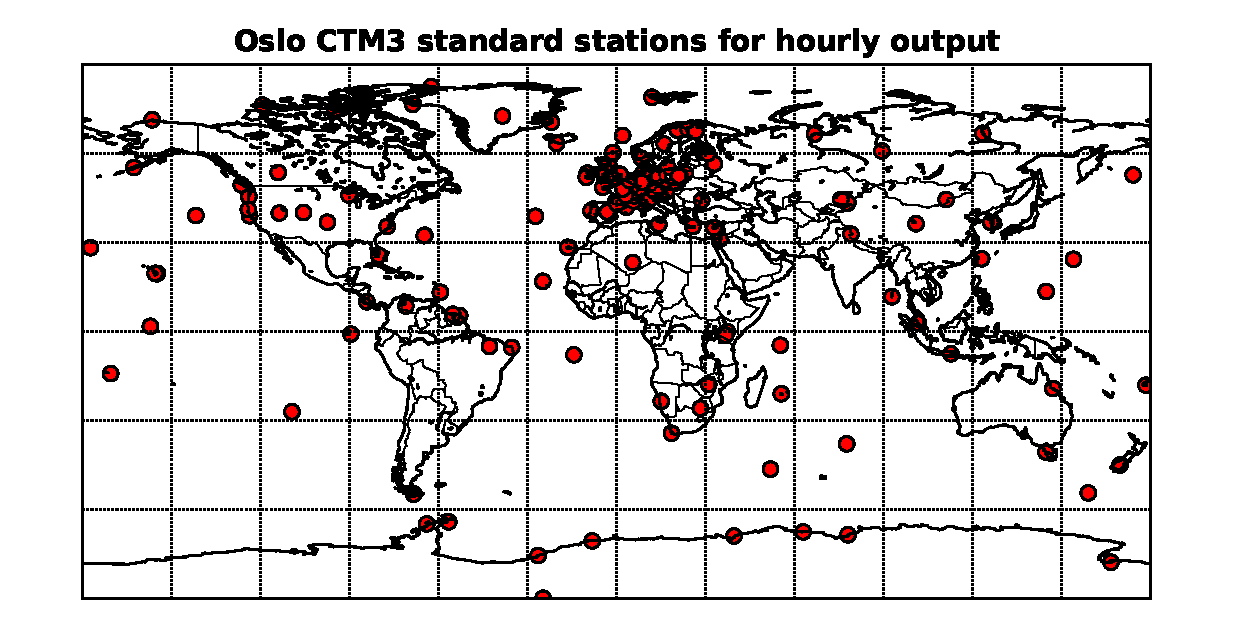
\includegraphics[width=0.97\linewidth]{figures/stations}
  \caption{Map of stations included in the standard output for
    vertical profiles.}
  \label{fig:vprofseriesmap}
\end{figure}



List of output data for each daily file:
\begin{itemize2}
  \item\texttt{year}: Year.
  \item\texttt{month}: Month of year.
  \item\texttt{date}: Date of month.
  \item\texttt{LPAR}: Number of vertical layers.
  \item\texttt{ntracer}: Number of tracers diagnosed.
  \item\texttt{nrofstations}: Number of stations.
  \item\texttt{NTHE}: Number of $\theta$-levels for equivalent latitude.
  \item\texttt{actual\_diag}: Number of \verb#NOPS# steps diagnosed, i.e.
    \verb#NROPSM * NRMETD#.
  \item\texttt{etaa}: Sigma coordinate A ($\eta_a$) for all levels.
  \item\texttt{etab}: Sigma coordinate B ($\eta_b$) for all levels.
  \item\texttt{stt\_components}: Tracer ID numbers diagnosed.
  \item\texttt{mole\_mass}: Molecular mass of tracers.
  \item\texttt{pvthe}: Theta levels for equivalent latitude.
\end{itemize2}
List of output data for each station:
\begin{itemize2}
  \item\texttt{locname}: Station name.
  \item\texttt{loccode}: Station 3-char code.
  \item\texttt{lat}: Latitude.
  \item\texttt{lon}: Longitude.
  \item\texttt{alt}: Altitude.
  \item\texttt{ii}: CTM zonal grid box index.
  \item\texttt{jj}: CTM meridional grid box index.
  \item\texttt{nb\_ii}: Zonal neighbor grid box index.
  \item\texttt{nb\_jj}: Meridional neighbor grid box index.
  \item\texttt{nb\_xfrac}: Fractional distance to zonal neighbor.
  \item\texttt{nb\_yfrac}: Fractional distance to meridional neighbor.
  \item\texttt{areaxy}: Grid box area [m$^2$] (interpolated).
\end{itemize2}
For all diagnostic steps, the following data are stored:
\begin{itemize2}
  \item\texttt{psfc}: Surface pressure [hPa].
  \item\texttt{BLH}: Boundary layer height [m].
  \item\texttt{mass}: Tracer masses [kg/grid box].
  \item\texttt{h2o}: H$_2$O mass [kg/grid box].
  \item\texttt{temperature}: Temperature [K].
  \item\texttt{airmass}: Air mass [kg/grid box].
  \item\texttt{zoflev}: Height of grid box bottoms [m].
  \item\texttt{eqlat}: Equivalent latitude on theta levels.
  \item\texttt{PVU}: Potential vorticity units.
  \item\texttt{tph\_pres}: Tropopause pressure [hPa].
\end{itemize2}




% Satellite vertical profiles
\subsubsection{Satellite vertical profiles}
\label{sxn:satprofs}
\index{diagnostics!Oslo CTM3!vertical profiles}\index{diagnostics!Oslo CTM3!satellite profiles}
A routine for putting out vertical profiles at given locations and times,
e.g.~satellite positions, are included in the file
{\it satelliteprofiles\_mls.f90}\index{source code!oslo!satelliteprofiles\_mls.f90}.
In this file you define which tracers to put out. Some meteorological
components are also diagnosed, e.g.~temperature, pressure, model grid height,
air mass, equivalent latitude, etc.
Using the satellite profile location (latitude and longitude), this
routine linearly interpolates horizontally from the 4~closest grid
boxes.
In the future, it may be better to save data for all columns and do
interpolation in post-processing. Due to the large amount of data per
file, this is not done now.

Since each profile is taken between some start time of \verb#NOPS# and start
time of \verb#NOPS+1#, output is given for both \verb#NOPS# and
\verb#NOPS+1#, allowing temporal interpolation as well.

List of output data for each daily file:
\begin{itemize2}
  \item\texttt{year}: Year.
  \item\texttt{month}: Month of year.
  \item\texttt{date}: Date of month.
  \item\texttt{LPAR}: Number of vertical layers.
  \item\texttt{ntracer}: Number of tracers diagnosed.
  \item\texttt{nsatprofs}: Number of profiles.
  \item\texttt{NTHE}: Number of $\theta$-levels for equivalent latitude.
  \item\texttt{etaa}: Sigma coordinate A ($\eta_a$).
  \item\texttt{etab}: Sigma coordinate B ($\eta_b$).
  \item\texttt{stt\_components}: Tracer ID numbers diagnosed.
  \item\texttt{mole\_mass}: Molecular mass of tracers.
  \item\texttt{pvthe}: Theta levels for equivalent latitude.
\end{itemize2}
List of output data for each profile:
\begin{itemize2}
  \item\texttt{time}: Time of observation.
  \item\texttt{time\_sec}: CTM \verb#NOPS# times before and after.
  \item\texttt{lat}: Latitude.
  \item\texttt{lon}: Longitude.
  \item\texttt{ii}: CTM zonal grid box index.
  \item\texttt{jj}: CTM meridional grid box index.
  \item\texttt{nb\_ii}: Zonal neighbor grid box index.
  \item\texttt{nb\_jj}: Meridional neighbor grid box index.
  \item\texttt{nb\_xfrac}: Fractional distance to zonal neighbor.
  \item\texttt{nb\_yfrac}: Fractional distance to meridional neighbor.
  \item\texttt{areaxy}: Grid box area [m$^2$] (interpolated).
\end{itemize2}
For the two closest \verb#NOPS# steps, the following data are stored:
\begin{itemize2}
  \item\texttt{psfc}: Surface pressure [hPa].
  \item\texttt{BLH}: Boundary layer height [m].
  \item\texttt{mass}: Tracer masses [kg/grid box].
  \item\texttt{H2O}: H$_2$O mass [kg/grid box].
  \item\texttt{temperature}: Temperature [K].
  \item\texttt{airmass}: Air mass [kg/grid box].
  \item\texttt{zoflev}: Height of grid box bottoms [m].
  \item\texttt{eqlat}: Equivalent latitude on theta levels.
  \item\texttt{PVU}: Potential vorticity units.
  \item\texttt{tph\_pres}: Tropopause pressure.
\end{itemize2}



% Ozone column
\subsubsection{O$_3$ column}
\label{sxn:o3_column}
\index{diagnostics!Oslo CTM3!ozone column}
Tropospheric and total columns of O$_3$ are diagnosed in the
subroutine {\it du\_columns}\index{subroutines!du\_columns} in
the file {\it diagnostics\_general.f90}\index{source code!oslo!diagnostics\_general.f90}.
It is called from {\it mp\_diag}\index{subroutines!mp\_diag},
which does diagnoses in each IJ-block.

The columns are diagnosed every meteorological time step (\verb#NMET#)
and are stored once every day. This is carried out in the routine
{\verb#write_ducolumns#}\index{subroutines!write\_ducolumns}.



% 3-hourly output
\subsubsection{3-hourly output}
\label{sxn:3hourlyoutput}
\index{diagnostics!Oslo CTM3!3-hourly output}\index{diagnostics!3-hourly output}
\model\ has the possibility of putting out 3-hourly instantaneous
fields, mostly O$_3$ and aerosols. These are e.g.~used for RF
calculations.

You turn this diagnose on by setting
\verb#LDUMP3HRS=.true.#\index{variables!LDUMP3HRS}
at the top of the file 
{\it gmdump3hrs.f90}\index{source code!oslo!gmdump3hrs.f90}, and the
main routine is \verb#dump3hrs#\index{subroutines!dump3hrs}.

If you want to add other components than O$_3$, this is of course
possible. When you understand the code, it should be easy to
implement.



% Snapshots on theta-levels
\subsubsection{Snapshots on $\theta$-levels}
\label{sxn:snapshot_theta}
\index{diagnostics!Oslo CTM3!snapshots on $\theta$-levels}
In the routine
\verb#write_snapshot_the#\index{subroutines!write\_snapshot\_the},
located in {\it diagnostics\_general.f90},
you can put out instantaneous mixing ratios of selected species, interpolated
to the potential temperature ($\theta$) levels defined in the physics routine,
see Section~\ref{sxn:eqlat}. The number of $\theta$-levels
(\verb#pvthe#\index{variables!pvthe}) are given by \verb#NTHE#.

Routine puts out data every hour, and the default species put out are
O$_3$ and N$_2$O, along with PVU and equivalent latitude.

Routine can put out data for only one hemisphere or both. See the source code
for how to change it.

The routine is called from \verb#nops_diag#, but is commented out by default.
A~second routine,
\verb#write_snapshot#\index{subroutines!write\_snapshot\_the}, is also
available, putting out gridbox mass of selected species on model levels.



% Emission tendencies
\subsubsection{Emission tendencies}
\label{sxn:emissiontendencies}
\index{diagnostics!Oslo CTM3!emission tendencies}
When emissions are treated as production terms in chemistry, i.e.~in
standard Oslo chemistry, the total emitted per day is calculated for
all species, in \verb#tnd_emis_daily#. This is explained in
Section~\ref{sxn:emissions_tnd}.





%%%%%%%%%%%%%%%%%%%%%%%%%%%%%%%%%%%%%%%%%%%%%%%%%%%%%%%%%%%%%%%%%%%%%%
%%%%%%%%%%%%%%%%%%%%%%%%%%%%%%%%%%%%%%%%%%%%%%%%%%%%%%%%%%%%%%%%%%%%%%






%%%%%%%%%%%%%%%%%%%%%%%%%%%%%%%%%%%%%%%%%%%%%%%%%%%%%%%%%%%%%%%%%%%%%%
%%%%%%%%%%%%%%%%%%%%%%%%%%%%%%%%%%%%%%%%%%%%%%%%%%%%%%%%%%%%%%%%%%%%%%
%%%%%%%%%%%%%%%%%%%%%%%%%%%%%%%%%%%%%%%%%%%%%%%%%%%%%%%%%%%%%%%%%%%%%%



%%%%%%%%%%%%%%%%%%%%%%%%%%%%%%%%%%%%%%%%%%%%%%%%%%%%%%%%%%%%%%%%%%%%%%
% Appendix -- #APPX
%%%%%%%%%%%%%%%%%%%%%%%%%%%%%%%%%%%%%%%%%%%%%%%%%%%%%%%%%%%%%%%%%%%%%%
\appendix



%%%%%%%%%%%%%%%%%%%%%%%%%%%%%%%%%%%%%%%%%%%%%%%%%%%%%%%%%%%%%%%%%%%%%%
% Description of model files -- #MODFILES
%%%%%%%%%%%%%%%%%%%%%%%%%%%%%%%%%%%%%%%%%%%%%%%%%%%%%%%%%%%%%%%%%%%%%%
\section{Description of model files}
\label{app:description_of_files}\index{files|see {source code}}
Here the source files are described. Generally, files inherited from
UCI are placed in the main directory, while the OSLO chemistry
and physics are placed in the directory \oslopath.
The files in the main directory is often referred to as the core files,
and will be described next.


% UCI core files
\subsection{UCI core source files}
\label{app:description_UCI_files}\index{source code!core}
The \model\ started out based on the \ucimodel\ version 5.6d, but was
later updated to \qcodelastupdate, before most of the UCI code was
restructured into Fortran90 free format, and all common blocks
were abandoned.
In this process I~renamed most of the files.
Future core update should be fairly straight-forward for a~somewhat
experienced user.

This Section describes the core files necessary to run the \model.
If you want to go back and see the UCI codes, you should contact UCI.

First the global variable files (common files) are listed, then the
core files are listed alphabetically.


% cmn_precision.f90
\subsubsection{\it cmn\_precision.f90}\index{source code!core!cmn\_precision.f90}
\label{app:core_precision}
This file defines the precision of the \model\ floating point variables.
Several are used:
\begin{itemize2}
  \item[r8] Double precision. Most variables use this.
  \item[r4] Single precision.
  \item[rMom] Precision of the second order moments.
    By default this is single precision.
  \item[rAvg] Precision of the global average arrays.
    By default this is single precision.
  \item[rTnd] Precision of the global tendency arrays.
    By default this is single precision.
\end{itemize2}


% cmn_size.F90
\subsubsection{\it cmn\_size.F90}\index{source code!core!cmn\_size.F90}
\label{app:core_size}
Contains the array size parameters and flags. Examples are
\verb#IPAR#\index{variables!IPAR},
\verb#IPARW#\index{variables!IPARW},
\verb#JPAR#\index{variables!JPAR},
\verb#JPARW#\index{variables!JPARW},
\verb#LPAR#\index{variables!LPAR},
\verb#LPARW#\index{variables!LPARW},
\verb#MPIPAR#\index{variables!MPIPAR},
\verb#MPJPAR#\index{variables!MPJPAR},
\verb#NRMETD#\index{variables!NRMETD},
\verb#NPAR#\index{variables!NPAR}, etc.


% cmn_parameters.f90
\subsubsection{\it cmn\_parameters.f90}\index{source code!core!cmn\_parameters.f90}
\label{app:core_parameters}
Contains chemical and physical parameters\index{parameters|see {variables}},
such as the Earth radius (\verb#A0#\index{variables!Earth radius, A0}),
Avogadro's number (\verb#AVOGNR#\index{variables!AVOGNR}),
Apparent molecular weight of dry air
(\verb#M_AIR#\index{variables!M\_AIR}),
gas constants (\verb#R_AIR#\index{variables!R\_AIR},
\verb#R_UNIV#\index{variables!R\_UNIV},
\verb#R_ATM#\index{variables!R\_ATM}),
and many more.
These are all listed in Table~\ref{table:parameters}.

\begin{table*}[ht!]
  \caption{Parameters defined in {\it cmn\_parameters.f90}.}
  \label{table:parameters}
  \begin{tabular}{l|l|l}
    Name & Value & Description\\
    \hline
    \verb#A0# & 6371000 & Earth radius [m]\index{variables!A0}\index{variables!Earth radius (A0)}\\
    \verb#G0# & 9.80665 & Gravitational constant [m/s$^2$]\index{variables!G0}\index{variables!gravitational constant (G0)}\\
    \verb#CPI#\index{variables!Pi} & 3.141592653589793 & $\pi$\\
    \verb#C2PI#\index{variables!C2PI} & \verb#2*CPI# & 2$\pi$\\
    \verb#CPI180#\index{variables!CPI180} & \verb#CPI/180# & Conversions to radians\\
    \verb#ZPI180#\index{variables!ZPI180} & \verb#1/CPI180# & Conversions from radians\\
    \hline
    \verb#atm2Pa#\index{variables!atm2Pa} & 101325 & Conversion from atmospheres to Pa\\
    \verb#Pa2atm#\index{variables!Pa2atm} & \verb#1/atm2Pa# & Conversion from Pa to atm\\
    \verb#J2kcal#\index{variables!J2kcal} & 4186.8 & Numbers of kcal in a~J\\
    \verb#M_AIR#\index{variables!M\_AIR} & 28.97 & Molecular mass for air [g/mol]\\
    \verb#R_UNIV#\index{variables!R\_UNIV} & 8.31446 & Universal gas constant [J/(K\,mol)] = [m$^3$*Pa/(K\,mol)]\\
    \verb#R_ATM#\index{variables!R\_ATM} & \verb#R_UNIV * Pa2atm# & Gas constant in [m$^3$*atm/(K\,mol)] ($\sim$8.205e-5)\\
    \verb#R_AIR#\index{variables!R\_AIR} & \verb#R_UNIV / M_AIR * 1000# & Specific gas constant for air [J/(K\,kg)] ($\sim$287)\\
    \verb#R_H2O#\index{variables!R\_H2O} & \verb#R_UNIV / 18.01528 * 1000# & Specific gas constant for water vapor [J/(K\,kg)] ($\sim$461)\\
    \verb#AVOGNR#\index{variables!AVOGNR} & \verb#6.022149e23# & Avogadro's number [molecules/mol]\\
    \verb#BOLTZMANN#\index{variables!BOLTZMANN} & \verb#1.38063e-23# & Boltzmann's const [J/(K\,molecules)]\\
    \verb#KBOLTZ#\index{variables!KBOLTZ} & \verb#1.e4 * BOLTZMANN# & Boltzmann's const [mb\,cm3/(K\,molecules)]\\
    \verb#cp_air#\index{variables!cp\_air} & 1004 & Specific heat of dry air at constant pressure [J/(K\,kg)\\
      \verb#Lv_0C#\index{variables!Lv\_0C} & \verb#2.501e6# & Latent heat of vaporization at 0$^{\circ}$C [J/kg]\\
      \verb#dLv_dT#\index{variables!dLv\_dT} & \verb#-0.00237e6# & Gradient of Lv between 0C and 100C [(J/kg)/K]\\
      & & \citep[Table C-5 in][]{Stull1988}\\
      \verb#TK_0C#\index{variables!TK\_0C} & 273.15 & Temperature [K] at 0$^{\circ}$C\\
      \verb#es_0C#\index{variables!es\_0C} & 611.2 & Saturation vapor pressure of H$_2$O at 0$^{\circ}$C [Pa]\\
      \verb#secDay#\index{variables!secDay} & 86400 & Seconds in a~day\\
      \verb#secYear#\index{variables!secYear} & 31536000 & Seconds in a~year\\
      \hline
      \verb#MINTEMP#\index{variables!MINTEMP} & 150 & Minimum temperature allowed in chemistry\\
      \verb#MAXTEMP#\index{variables!MAXTEMP} & 350 & Maximum temperature allowed in chemistry\\
      \verb#TEMPRANGE#\index{variables!TEMPRANGE} & \verb#MAXTEMP - MINTEMP# & Temperature range.\\
      \hline
      \verb#LDEBUG#\index{variables!LDEBUG} & .true. & Global flag for including more extensive debugging.\\
      \hline
  \end{tabular}
\end{table*}


% cmn_ctm.f90
\subsubsection{\it cmn\_ctm.f90}\index{source code!core!cmn\_ctm.f90}
\label{app:core_ctm}
Defines the main arrays for the transport model, such as
\verb#STT#\index{variables!STT} and the moments
(\verb#SUT#\index{variables!SUT}, \verb#SVT#\index{variables!SVT},
\verb#SWT#\index{variables!SWT}, \verb#SUU#\index{variables!SUU},
\verb#SVV#\index{variables!SVV}, \verb#SWW#\index{variables!SWW},
\verb#SUV#\index{variables!SUV}, \verb#SUW#\index{variables!SUW}, 
\verb#SVW#\index{variables!SVW}).

Also grid info such as longitude\index{longitude}
(\verb#XGRD#\index{variables!XGRD},
\verb#XDGRD#\index{variables!XDGRD},
\verb#XEDG#\index{variables!XEDG},
\verb#XDEDG#\index{variables!XDEDG}),
latitude
(\verb#YGRD#\index{variables!YGRD},
\verb#YDGRD#\index{variables!YDGRD},
\verb#YEDG#\index{variables!YEDG},
\verb#YDEDG#\index{variables!YDEDG}),
and sigma hybrid coordinates
(\verb#ETAA#\index{variables!ETAA}, \verb#ETAAW#
\verb#ETAB#\index{variables!ETAB}, \verb#ETABW#)
are defined here.


% cmn_chem.f90
\subsubsection{\it cmn\_chem.f90}\index{source code!core!cmn\_chem.f90}
\label{app:core_chem}
Defines the main arrays for emissions and chemistry, such as
\verb#E3DSNEW(LPAR,IPAR,JPAR,E3PAR)#\index{variables!E3DSNEW} and the
tables mapping species to emission datasets:
\begin{itemize2}
  \item \verb#NE2TBL#\index{subroutines!NE2TBL}:
    Total number of 2D emission datasets.
  \item \verb#NM2TBL#\index{subroutines!NM2TBL}:
    Table of months the emissions apply for.
  \item \verb#NY2TBL#\index{subroutines!NM2TBL}:
    Table of months the emissions apply for.
  \item \verb#E2DS#\index{subroutines!E2DS}:
    All 2D emission datasets.
  \item \verb#E2LTBL#\index{subroutines!E2LTBL}:
    Table mapping species to 2D emission datasets.
  \item \verb#E2STBL#\index{subroutines!E2STBL}:
    Table of scaling factors for the mapping of each species
    and 2D emission datasets.
\end{itemize2}
Similar arrays exist for 3D emissions.

Here you also find
the tracer name \verb#TNAME#\index{variables!TNAME},
tracer molecular weight \verb#TMASS#\index{variables!TMASS},
and other variables such as conversion factors
\verb#TMASSMIX2MOLMIX#\index{variables!TMASSMIX2MOLMIX} and
\verb#TMOLMIX2MASSMIX#\index{variables!TMOLMIX2MASSMIX}.

The variables are generally well described in the source code.


% cmn_diag.f90
\subsubsection{\it cmn\_diag.f90}\index{source code!core!cmn\_diag.f90}
\label{app:core_diag}
Defines arrays for diagnostics, such as
\verb#STTAVG#\index{variables!STTAVG},
\verb#AIRAVG#\index{variables!AIRAVG},
\verb#JDO_A#\index{variables!JDO\_A}.


% cmn_fjx.f90
\subsubsection{\it cmn\_fjx.f90}\index{source code!core!cmn\_fjx.f90}
\label{app:core_fjx}
Defines fast-JX parameters and arrays.


% cmn_met.f90
\subsubsection{\it cmn\_met.f90}\index{source code!core!cmn\_met.f90}
\label{app:core_met}
Defines meteorological arrays.


% cmn_sfc.f90
\subsubsection{\it cmn\_sfc.f90}\index{source code!core!cmn\_sfc.f90}
\label{app:core_sfc}
Defines surface variables such as land surface type
(\verb#landSurfTypeFrac#\index{variables!landSurfFracType}),
land-sea mask
(\verb#LSMASK#\index{variables!LSMASK}),
and dry deposition velocity 
(\verb#VDEP#\index{variables!VDEP}).


% averages.f90
\subsubsection{\it averages.f90}
\label{app:core_averages}\index{source code!core!averages.f90}
Contains routines for summing up 3D averages.
\begin{itemize2}
  \item \verb#AVG_WRT_NC4#\index{subroutines!AVG\_WRT\_NC4}:
    Write core 3D averages (the avgsav-files\index{avgsav-files}),
    including \verb#XSTT# averages, surface pressure averages
    (which is 2D), and some meteorological averages.
  \item \verb#AVG_ADD2#\index{subroutines!AVG\_ADD2}:
    Add to 3D averages.
  \item \verb#AVG_CLR2#\index{subroutines!AVG\_CLR2}:
    Clear 3D averages.
  \item \verb#AVG_P1#\index{subroutines!AVG\_P1}:
    Write 1D averages to screen.
  \item \verb#AVG_WRT2#\index{subroutines!AVG\_WRT2}:
    Only included for history. See \verb#AVG_WRT_NC4#.
    Write core 3D averages (the avgsav-files\index{avgsav-files}),
    including \verb#XSTT# averages, surface pressure averages
    (which is 2D), and several meteorological averages.
\end{itemize2}


% budgets.f90
\subsubsection{\it budgets.f90}
\label{app:core_budgets}\index{source code!core!budgets.f90}
Contains routines for summing up tendency budgets.
\begin{itemize2}
  \item \verb#TBGT_G#\index{subroutines!TBGT\_G}:
    Clear budget arrays.
  \item \verb#TBGT_L#\index{subroutines!TBGT\_L}:
    Accumulate budgets layerwise.
  \item \verb#TBGT_IJ#\index{subroutines!TBGT\_IJ}:
    Accumulate budgets in IJ-block.
  \item \verb#TBGT_P0#\index{subroutines!TBGT\_P0}:
    0D print to screen.
  \item \verb#TBGT_P1#\index{subroutines!TBGT\_P1}:
    1D print to screen.
  \item \verb#TBGT_P2#\index{subroutines!TBGT\_P2}:
    2D print to screen.
\end{itemize2}


% cloudjx.f90
\subsubsection{\it cloudjx.f90}
\label{app:core_cloudjx}\index{source code!core!cloudjx.f90}
Routines for treating cloud-J.
%TOBEUPDATED
Currently set up for cloud2 as used by fast-JX 6.7c, but will
be updated when fast-JX 7.3c is included.
\begin{itemize2}
  \item \verb#cloud_init#\index{subroutines!cloud\_init}:
    Initialise cloud-J.
  \item \verb#RANSET#\index{subroutines!RANSET}:
    Set random number. Random seed is
    \verb#RANSEED#\index{variables!RANSEED}, which is set in
    \maininput.
\end{itemize2}

Some important variables for cloud2:
\begin{itemize2}
  \item \verb#LCLDAVG#\index{variables!LCLDAVG}:
  \item \verb#LCLDQMD#\index{variables!LCLDQMD}:
  \item \verb#LCLDQMN#\index{variables!LCLDQMN}:
  \item \verb#LCLDRANA#\index{variables!LCLDRANA}:
  \item \verb#LCLDRANA#\index{variables!LCLDRANA}:
\end{itemize2}



% convection.f90
\subsubsection{\it convection.f90}
\label{app:core_convection}\index{source code!core!convection.f90}
This is the f90 version of the UCI {\it p-cnvw.f}. It has been modified
to \model, calculating elevator fractions, and also the Henry coefficients
used in convective washout.
A~new convective wet loss variable is
included; \verb#CNV_WETL(LPAR,NPAR)#\index{variables!CNV\_WETL}.

\begin{itemize2}
  \item \verb#CONVW_OSLO#\index{subroutines!CONVW\_OSLO}:
    The main routine.
  \item \verb#ADJFLX2#\index{subroutines!ADJFLX2}:
    Adjust convective fluxes so that no more than a~fraction
    of the grid box mass is moved each time step.
  \item \verb#ADJFLX# Old version of \verb#ADJFLX2#.
  \item \verb#QCNVW2_OSLO#\index{subroutines!QCNVW2\_OSLO}:
    Column model calculating convective transport, and also
    convective scavenging by updrafts.
  \item \verb#QCNVW2#: UCI routine kept for history.
  \item \verb#SCAV_UPD#: UCI routine kept for history.
\end{itemize2}




% fastjx.f90
\subsubsection{\it fastjx.f90}\index{source code!core!fastjx.f90}
\label{app:core_fastjx}
%TOBEUPDATED
Contains routines for fastJX, except the main driver which is so far located
in {\it p-phot\_oc.f}. That will change when fast-JX is updated to 7.3.
\begin{itemize2}
  \item \verb#RD_XXX#\index{subroutines!RD\_XXX}: Reads {\it FJX\_spec.dat}.
  \item \verb#RD_MIE#\index{subroutines!RD\_MIE}: Reads \fjxscatfile.
  \item \verb#RD_JS#\index{subroutines!RD\_JS}:
    Reads \ratjfile\ file.
  \item \verb#RD_O1D#\index{subroutines!RD\_O1D}:
    Reads \verb#O1D# entry of \ratjfile\ file.
  \item \verb#SET_ATM#\index{subroutines!SET\_ATM}:
    Reads O$_3$ and temperature climatologies to use above the model
    domain. It can possibly be used in the stratosphere when stratospheric
    chemistry in not included, but \model\ uses its own climatology
    for that. Sets e.g. \verb#TOPT#\index{variables!TOPT},
    \verb#TOPM#\index{variables!TOPM},
    \verb#TOP3#\index{variables!TOP3}.
\end{itemize2}

{\it Changes compared to UCI p-phot.f file}\\
In the subroutine \verb#PHOT_IN# a~small piece of ASAD code was
removed. Some other ASAD variables has been removed.

Also, the subroutine \verb#SET_ATM# had to be modified to include
climatology data for the uppermost layer (\verb#LPAR3#, \verb#LPART#
and \verb#LPARM#).


% grid.f90
\subsubsection{\it grid.f90}
\label{app:core_grid}\index{source code!core!grid.f90}
Routines for setting up model grid.
\begin{itemize2}
  \item \verb#SET_GRID#\index{subroutines!SET\_GRID}:
    Sets up global grid, such as latitude, longitude,
    area of grid boxes, etc.
  \item \verb#LABELG#\index{subroutines!LABELG}:
    For printing grid info to screen.
  \item \verb#DIAGBLK#\index{subroutines!DIAGBLK}:
    Finds grid box start/end indices for box diagnose.
  \item \verb#DIAG_LTSTN#\index{subroutines!DIAG\_LTSTN}:
    Finds grid box indices for station diagnose.
  \item \verb#DIAG_LTGL#\index{subroutines!DIAG\_LTGL}:
    Finds grid box indices for local time station diagnose.
  \item \verb#GAUSST2#\index{subroutines!GAUSST2}:
    Calculate Gaussian quadrature points and weights.
  \item \verb#DBLDBL#\index{subroutines!DBLDBL}:
    Define longitude and latitude of horizontally degraded
    grid.
  \item \verb#AIRSET#\index{subroutines!AIRSET}:
    Sets up 3D air mass.
  \item \verb#SURF_IN#\index{subroutines!SURF\_IN}:
    Reads land fraction datasets.
  \item \verb#gridICAO#\index{subroutines!gridICAO}:
    Not used. I think this finds grid for some ICAO emission
    data.
\end{itemize2}


% initialize.f90
\subsubsection{\it initialize.f90}\index{source code!core!initialize.f90}
\label{app:core_initialize}
Routines for initializing the \model.
\begin{itemize2}
  \item \verb#INPUT#\index{subroutines!INPUT}:
    Reads \maininput.
  \item \verb#SETUP_SPECIES#\index{subroutines!SETUP\_SPECIES}:
    Reads restart file.
  \item \verb#SETUP_UNF_OUTPUT#\index{subroutines!SETUP\_UNF\_OUTPUT}:
    Opens unformatted output files (UCI heritage).
  \item \verb#report_zeroinit#\index{subroutines!report\_zeroinit}:
    Reports which tracers are initialized to zero
    (i.e.~not read from file).
\end{itemize2}


% lightning.f90
\subsubsection{\it lightning.f90}\index{source code!core!lightning.f90}
\label{app:core_lightning}
Contains routines for calculating lightning NOx (L-NOx) emissions.
There are several methods for doing this, as described in
Section~\ref{sxn:emissions_lightning}.
\begin{itemize2}
  \item \verb#getScaleFactors#\index{subroutines!getScaleFactors}:
    Sets scaling factors based on which meteorological dataset is
    used.
  \item \verb#LIGHTNING_OAS2015#\index{subroutines!LIGHTNING\_OAS2015}:
    Default method for calculating L-NOx.
  \item \verb#LIGHTNING_GMD2012#\index{subroutines!LIGHTNING\_GMD2012}:
    L-NOx as described by \citet{SovdeEA2012}.
  \item \verb#LIGHTNING_UCI2015#\index{subroutines!LIGHTNING\_UCI2015}:
    L-NOx as used by UCI-CTM in 2015. I~do not recommend using this.
  \item \verb#LIGHTDIST#\index{subroutines!LIGHTDIST}:
    Sets up vertical distribution of L-NOx.
  \item \verb#filterLNC#\index{subroutines!filterLNC}:
    Filter convective mass fluxes to reduce noise in L-NOx horizontal
    distribution.
  \item \verb#distland#\index{subroutines!distland}:
    Finds grid boxes that are land or have land in 300\,km
    proximity. Test routine to make land near-land lightning
    behaving like land. {\bf Not used.}
  \item \verb#LIGHTNING_ALLEN2002#\index{subroutines!LIGHTNING\_ALLEN2002}:
    L-NOx as described by \citet{AllenPickering2002}. Not evaluated.
\end{itemize2}


% metdata_ecmwf.f90
\subsubsection{\it metdata\_ecmwf.f90}\index{source code!core!metdata\_ecmwf.f90}
\label{app:core_metdataecmwfnc}
Read-in for ECMWF IFS meteorological data on netCDF4 format.

\begin{itemize2}
  \item \verb#update_metdata#\index{subroutines!update\_metdata}:
    Updates meteorological data.
  \item \verb#fluxfilter2#\index{subroutines!fluxfilter2}:
    Filter convective mass fluxes; removes noise.
  \item \verb#data2mpblocks#\index{subroutines!data2mpblocks}:
    Puts globally gridded (\verb#IPAR,JPAR#) data into IJ-block
    (\verb#IDBLK,JDBLK,MPBLK#).
  \item \verb#gotData#\index{subroutines!gotData}: Prints info to standard out.
  \item \verb#skipData#\index{subroutines!skipData}: Prints info to standard out.
\end{itemize2}


% metdata_ecmwf_uioformat.f90
\subsubsection{\it metdata\_ecmwf\_uioformat.f90}\index{source code!core!metdata\_ecmwf\_uioformat.f90}
\label{app:core_metdataecmwfuio}
Traditional read-in for ECMWF IFS meteorological data on UIO binary format.


% omp.f90
\subsubsection{\it omp.f90}
\label{app:core_omp}\index{source code!core!omp.f90}
Routines for switching between global and IJ-block structures.
Slightly modified compared to UCI routines, e.g.~looping is
changed to reduce striding.
\begin{itemize2}
  \item \verb#MPSPLIT#\index{subroutines!MPSPLIT}:
    Split global arrays into IJ-block arrays.
  \item \verb#MPBIND#\index{subroutines!MPBIND}:
    Convert back to global arrays.
  \item \verb#get_iijjmp#\index{subroutines!get\_iijjmp}:
    From global indices \verb#I,J#, find IJ-block indices
    \verb#II,JJ,MP#. Not really necessary because of the array
    \verb#all_mp_indices#\index{variables!all\_mp\_indices}
    and the next routine:
  \item \verb#get_all_mpind#\index{subroutines!get\_all\_mpind}:
    Sets up array
    \verb#all_mp_indices#\index{variables!all\_mp\_indices}
    to map global indices to IJ-block indices.\\
    \verb#all_mp_indices(1,I,J)=II#\\
    \verb#all_mp_indices(2,I,J)=JJ#\\
    \verb#all_mp_indices(3,I,J)=MP#
\end{itemize2}


% pbl_mixing.f90
\subsubsection{\it pbl\_mixing.f90}
\label{app:core_pblmixing}\index{source code!core!pbl\_mixing.f90}
Routines for calculating planetary boundary layer (PBL) mixing.
This is the f90 version of the UCI file {\it p-pbl.f}, but modified
to use the scheme by \citet{HoltslagEA1990}.
\begin{itemize2}
  \item \verb#CNVBDL#\index{subroutines!CNVBDL}:
    Main routine for calculating PBL mixing.
  \item \verb#BULK#\index{subroutines!BULK}:
    Prather bulk scheme.
  \item \verb#get_keddy_L1#\index{subroutines!get\_keddy\_L1}:
    Calculates diffusivity in the lowermost model layer, as done in
    the routine \verb#KPROF#.
  \item \verb#KPROF2#\index{subroutines!KPROF2}:
    Calculates diffusivity of heat used in PBL closure, as used by
    the \citet{HoltslagEA1990} scheme. Should be used instead of
    \verb#KPROF#, since unnecessary calculations have been removed.
  \item \verb#KPROF#\index{subroutines!KPROF}:
    Calculates diffusitivities used in PBL closure, as used by
    the \citet{HoltslagEA1990} scheme.
  \item \verb#PHIM#\index{functions!PHIM}:
    Calculates similarity theory stability correction for momentum.
  \item \verb#PHIH#\index{functions!PHIH}:
    Calculates similarity theory stability correction for heat.
  \item \verb#TRIDIAG#\index{subroutines!TRIDIAG}:
    Solves tri-diagonal system.
  \item \verb#INTERP#\index{subroutines!INTERP}:
    Mass weighted interpolation routine to determine PBL profiles
    from similarity. Ekman solution.
  \item \verb#QXZON#\index{subroutines!QXZON}:
    Combines mass boxes into extended zones.
  \item \verb#QZONX#\index{subroutines!QZONX}:
    Divides one extended zone into equal-mass boxes.
\end{itemize2}


% pmain.f90
\subsubsection{\it pmain.f90}\index{source code!core!pmain.f90}
\label{app:core_pmain}
The main program \pmainf\ has been modified for the \model.
Input routines are changed and also some calls to master routines.
There is also an internal chemistry loop of max 15\,minutes for the
processes mixing/emissions/chemistry/deposition.
This is to reduce the large changes imposed by emissions and
deposition. For large deposition values, all of a~tracer can be
removed at the surface if the time step is too long. For a~16\,m
layer, a~deposition velocity of 1.77\,cm/s will remove everything in
15\,minutes. Linoz calls has been removed.

See Section~\ref{sxn:internal_chem_loop} for more.


% regridding.f90
\subsubsection{\it regridding.f90}\index{source code!core!regridding.f90}
\label{app:core_regridding}
Routines for regridding data.
\begin{itemize2}
  \item \verb#E_GRID#\index{subroutines!E\_GRID}:
    Regridding of 2D horizontal field.
    Field must {\bf not} be per area, i.e. concentrations and
    mixing ratios must be multiplied by area before interpolation,
    and divided by new area afterwards.
    Handles emission dataset which include moments (usually not
    used in \model).
    \verb#XBEDG# and \verb#XDEDG# may have shift at dateline.
    \verb#YBEDG# and \verb#YDEDG# must start at 90S.
  \item \verb#E_GRID_Y#\index{subroutines!E\_GRID\_Y}:
    Regridding of array in meridional direction.
  \item \verb#TRUNG8#\index{subroutines!TRUNG8}:
    Convert double precision (\verb#r8#) field from native resolution
    to degraded horizontal resolution.
  \item \verb#TRUNG4#\index{subroutines!TRUNG4}:
    Convert single precision (\verb#r4#) field from native resolution
    to degraded horizontal resolution.
\end{itemize2}


% source_uci.f90
\subsubsection{\it source\_uci.f90}\index{source code!core!source\_uci.f90}
\label{app:core_sourceuci}
\begin{itemize2}
  \item \verb#SOURCE#\index{subroutines!SOURCE}:
    Routine for adding emissions to emission array each time step, when
    treated as a~separate process (i.e.~not as production term in
    chemistry).\\
    {\bf Not tested with Oslo chemistry}.\\
    When treated as chemistry production term, the routine
    \verb#emis4chem# in {\it emisdep4chem\_oslo.f90} is used
    (see Appendix~\ref{app:emisdep4chem_oslo}).
\end{itemize2}


% scavenging_largescale_uci.f90
\subsubsection{\it scavenging\_largescale\_uci.f90}
\label{app:core_scavls}\index{source code!core!scavenging\_largescale\_uci.f90}
Large scale scavenging as described in Section~\ref{sxn:ls_scav}.
Some modifications from \model\ are implemented.

\begin{itemize2}
  \item \verb#WASHO#\index{subroutines!WASHO}:
    Master routine calling \verb#WASH1# or \verb#WASH2#.
  \item \verb#WASH1#\index{subroutines!WASH1}:
    Simple UCI wet scavenging routine.
    Kept for history; should not be used.
  \item \verb#WASH2#\index{subroutines!WASH2}:
    Routine by \citet{NeuPrather2012}, partly modified for \model.
  \item \verb#DISGAS#\index{subroutines!DISGAS}:
    Calculates the mass of tracer dissolved in aqueous phase.
    Uses the flag \verb#IT258K#\index{variables!IT258K} to
    define how to use Henry's law.
  \item \verb#HENRYS#\index{subroutines!HENRYS}:
    Use Henry's law to calculate mass dissolved in aqueous phase.
    No dissolved tracer below 258\,K, and uses retention
    coefficient\index{retention coefficient} between
    258\,K and 273\,K.
  \item \verb#HENRYSallT#\index{subroutines!HENRYSallT}:
    Same as \verb#HENRYS#, but uses retention coefficient also
    below 258\,K.
  \item \verb#RAINGAS#\index{subroutines!RAINGAS}:
    Calculates tracer (kg) picked up by {\it new} rain.
  \item \verb#WASHGAS#\index{subroutines!WASHGAS}:
    Calculates tracer picked up by falling precipitation (kg)
    and also evaporated from precipitation (kg).
  \item \verb#DIAMEMP#\index{subroutines!DIAMEMP}:
    Empirical fit of precipitation diameter to cloud water
    density and rain rate, following \citet{FieldHeymsfield2003}.
  \item \verb#GAMMAX#\index{subroutines!GAMMAX}:
    Calculates gamma using ln gamma algorithm.
  \item \verb#WETSET_CTM3#\index{subroutines!WETSET\_CTM3}:
    Initialises and sets wet scavenging parameters for \model.
\end{itemize2}


% spectral_routines.f
\subsubsection{\it spectral\_routines.f}
\label{app:core_spectral}\index{source code!core!spectral\_routines.f}
Spectral routines, not collected as module. These are purely inherited
from UCI/\oldmodel.
\begin{itemize2}
  \item \verb#SPE2GP#\index{subroutines!SPE2GP}:
    Converts spectral field to gridded field.
  \item \verb#ZD2UV#\index{subroutines!ZD2UV}:
    Converts spectral fields of vorticity and divergence to
    gridded field of zonal wind (\verb#U#) and meridional wind
    (\verb#V#).
  \item \verb#UVCOEF#\index{subroutines!UVCOEF}:
    Used by \verb#ZD2UV# to calculate spectral coefficients.
  \item \verb#FFT_99#\index{subroutines!FFT\_99}:
    Multiple fast real periodic transform of length N performed
    by removing redundant operations from complex transform
    length N.
  \item \verb#FFT_RPASS#\index{subroutines!FFT\_RPASS}:
    Performs one pass-thru data as part of multiple FFT
    (\verb#FFT_99#).
  \item \verb#FFT_DDSS#\index{subroutines!FFT\_DDSS}:
    Calculate constant arrays needed for evaluating spectral
    coefficients for \verb#U# and \verb#V# from vorticity
    and divergence.
  \item \verb#FFT_SET#\index{subroutines!FFT\_SET}:
    Computes factors of N and trigonometric functions needed
    by \verb#FFT_99#
  \item \verb#LEGGEN#\index{subroutines!LEGGEN}:
    Calculate Legendre functions.
  \item \verb#GAUSST#\index{subroutines!GAUSST}:
    Old routine for calculating Gaussian quadrature points and
    weights. Use \verb#GAUSST2# ({\it grid.f90}) instead.
\end{itemize2}


% steflux.f90
\subsubsection{\it steflux.f90}\index{source code!core!steflux.f90}
\label{app:core_steflux}
Routines for calculating stratosphere-troposphere exchange (STE)
as explained in Section~\ref{sxn:ste}.
This is the f90 version of UCI code {\it p-chemflux.f}.
\begin{itemize2}
  \item \verb#CHEMFLUX#\index{subroutines!CHEMFLUX}:
    Saves the horizontal flux of specified tracer (usually O$_3$) in
    the troposphere, but only for tropospheric to tropospheric boxes.
  \item \verb#CHEMFLUX_E90#\index{subroutines!CHEMFLUX\_E90}:
    Finds horizontal fluxes within the troposphere based
    on e90-tracer.
  \item \verb#dumpuvflux#\index{subroutines!dumpuvflux}:
    Accumulates horizontal fluxes into 3D arrays. Accumulates over
    time period defined by flux calendar
    (\verb#JDO_X#\index{variables!JDO\_X}).
  \item \verb#DUMPTRMASS#\index{subroutines!DUMPTRMASS}:
    Accumulates tropospheric mass of tracer (O$_3$).
  \item \verb#DUMPTRMASS_E90#\index{subroutines!DUMPTRMASS\_E90}:
    Accumulates tropospheric mass of tracer (O$_3$) based on e90 tracer.
  \item \verb#SAVETRMASS#\index{subroutines!SAVETRMASS}:
    Saves daily average mass of tracer (O$_3$).
  \item \verb#STEBGT_CLR#\index{subroutines!STEBGT\_CLR}:
    Clears STE diagnostics.
  \item \verb#STEBGT_WRITE#\index{subroutines!STEBGT\_WRITE}:
    Writes STE budget to netCDF4 file.
  \item \verb#ctm3_pml#\index{subroutines!ctm3\_pml}:
    Calculates tendency (production minus loss; PML) below
    predefined O$_3$ surfaces.
  \item \verb#ctm3_o3scav#\index{subroutines!ctm3\_o3scav}:
    Calculates net scavenged O$_3$ below predefined O$_3$ surfaces.
  \item \verb#chemflux_setup#\index{subroutines!chemflux\_setup}:
    Set up STE diagnostics.
\end{itemize2}



% stt_save_load.f90
\subsubsection{\it stt\_save\_load.f90}
\label{app:stt_save_load}\index{source code!core!stt\_save\_load.f90}
Contains routines to save and load STT from restart files.
\begin{itemize2}
  \item \verb#load_restart_file#\index{subroutines!load\_restart\_file}:
    Restart from netCDF4 files saved by \verb#save_restart_file#.
    Setting argument \verb#MODE# to zero will read the main restart
    file (also setting AIR), while non-zero will read additional fields
    from specified files. This has to be hard-coded in the subroutine
    \verb#SETUP_SPECIES#\index{subroutines!SETUP\_SPECIES} in the file
    {\it initialize.f90}\index{source code!core!initialize.f90}.    
  \item \verb#getField_and_interpolate#\index{subroutines!getField\_and\_interpolate}:
    This routine is bound to \verb#load_restart_file#, and reads
    a~3D field from a~netCDF4 file, with \verb#ncid# as file id and
    \verb#var_id# as variable id.
    If resolution on file differs from model resolution, the field is
    interpolated to model resolution.
    Vertical interpolation is not possible yet.
  \item \verb#save_restart_file#\index{subroutines!save\_restart\_file}:
    Saves netCDF4 restart file. Contains variables necessary for
    restarting a~run, as well as useful variables for other purposes.
    Transported species have prefix \verb#STT_#,
    and for these species there are also moments available, having
    prefixes
    \verb#SUT_#, \verb#SVT_#, \verb#SWT_#, \verb#SUU_#, \verb#SVV_#,
    \verb#SWW_#, \verb#SUV_#, \verb#SUW_#, \verb#SVW_#.
    Non-transported species have prefix \verb#XSTT_#.
% Old versions
  \item \verb#OSLO_CON_RUN#\index{subroutines!OSLO\_CON\_RUN}:
    Restart from files saved by \verb#OC_CON_SAV#.
    Setting argument \verb#MODE# to zero will read the main restart
    file, while non-zero will read additional fields from any
    specified file.
    Must match model resolution.
  \item \verb#OSLO_CON_SAV#\index{subroutines!OSLO\_CON\_SAV}:
    Old routine for saving restart file; instant fields, component by component.
    Called based on input file flag \verb#JDO_C#\index{variables!JDO\_C}.
    The restart file also contains grid info to use when e.g.~interpolating
    to other resolutions.
    Should not be used.
  \item \verb#restart_from_CTM3avg#\index{subroutines!restart\_from\_CTM3avg}:
    Starts from \model\ {\it avgsavDDDDD.dta} files, version~7.
    Reads the file {\it avgsav\_input} (no extension), so you must rename
    the input file accordingly.
    Must match model resolution.
  \item \verb#restart_from_CTM3avg_T42#\index{subroutines!restart\_from\_CTM3avg\_T42}:
    Same as \verb#restart_from_CTM3avg#, but reads T42 resolution
    {\it avgsavDDDDD} files and interpolates to current resolution.
    It reads the file {\it avgsav\_input} (no extension).
  \item \verb#OSLO_CON_RUN42#\index{subroutines!OSLO\_CON\_RUN42}:
    Reads \model\ T42 resolution restart file, and interpolates to
    current resolution. Works on sav-files version~1 and~2.
  \item \verb#OSLO_CON_RUNxx#\index{subroutines!OSLO\_CON\_RUNxx}:
    Reads any \model\ resolution restart file, and interpolates to
    current resolution. Requires that the sav-file is version~2 or
    higher. Will stop if model resolution is the same as on file,
    because not all moments are used.
  \item \verb#OSLO_RESTARTFILE_INFO#\index{subroutines!OSLO\_RESTARTFILE\_INFO}:
    Retrieves resolution info from the old binary restart files.
\end{itemize2}


% utilities.f90
\subsubsection{\it utilities.f90}
\label{app:utilities}\index{source code!core!utilities.f90}
Various utilities for \model. More utilities are given in
{\it utilities\_oslo.f90}.
\begin{itemize2}
  \item \verb#write_log#\index{subroutines!write\_log}:
    Writes start and end of model to screen.
  \item \verb#model_info#\index{subroutines!model\_info}:
    Prints info about run to screen.
  \item \verb#calendar#\index{subroutines!calendar}:
    Calculates day counters, but also some info about next time step,
    such as \verb#JYEAR_NEXT#, \verb#JMON_NEXT#, \verb#JDAY_NEXT#,
    \verb#JDATE_NEXT#.
  \item \verb#is_leap#\index{subroutines!is\_leap}:
    Calculates whether a~year is leap year or not.
  \item \verb#get_soldecdis#\index{subroutines!get\_soldecdis}:
    Calculates solar declination and distance to Sun.
    Same as originally found in \verb#CALENDR#.
  \item \verb#CALENDR_OLD#\index{subroutines!CALENDR\_OLD}:
    Old routine to calculate day counters and also solar declination
    and distance to Sun. Not used.
  \item \verb#CALENDL#\index{subroutines!CALENDL}:
    Looks up calendar and checks for flags.
  \item \verb#LOCSZA#\index{subroutines!LOCSZA}:
    Calculates cosine of local solar zenith angle, and the
    solar flux factor.
  \item \verb#LCM#\index{subroutines!LCM}:
    Calculates the least common multiple of two numbers.
  \item \verb#ctmExitC#\index{subroutines!ctmExitC}:
    Exit routine printing message.
  \item \verb#ctmExitL#\index{subroutines!ctmExitL}:
    Exit routine printing message and label.
  \item \verb#ctmExitIJL#\index{subroutines!ctmExitIJL}:
    Exit routine printing message and \verb#I,J,L#.
  \item \verb#get_free_fileid#\index{functions!get\_free\_fileid}:
    Finds a~free file id number.
  \item \verb#get_dinm#\index{subroutines!get\_dinm}:
    Returns the number of days in months, depending on whether
    year is leap year or not.
  \item \verb#CFRMIN#\index{subroutines!CFRMIN}:
    Set minimum limit on cloud fraction.
  \item \verb#CIWMIN#\index{subroutines!CIWMIN}:
    Set minimum limit on in-cloud water and ice ratios (kg/kg).
  \item \verb#check_btt#\index{subroutines!check\_btt}:
    Checks \verb#BTT# array for negatives and NaNs.
    Allows tracer id 110 (sum of oxygen, SO) to be negative.
  \item \verb#adjust_moments#\index{subroutines!adjust\_moments}:
    Scales down moments if \verb#BTT# has been reduced during
    a~process (if it is smaller than \verb#BTTBCK#).
\end{itemize2}




% p-cloud2.f
\subsubsection{\it p-cloud2.f}\index{source code!core!p-cloud2.f}
\label{app:core_cloud2}
Routines for calculating cloud2\index{cloud2}.
%TOBEUPDATED
Will be updated when cloud-J is included.
\begin{itemize2}
  % OSLO_CON_SAV
  \item \verb#CLOUD#\index{subroutines!CLOUD}:
    Calculates cloud properties.
  \item \verb#QUADCA#\index{subroutines!QUADCA}:
    Generates 4 quadrature independent column atmospheres
    (ICAs)\index{independent column atmospheres}\index{ICA}.
  \item \verb#OD_LIQ#\index{subroutines!OD\_LIQ}:
    Sets effective radius and extinction for liquid clouds.
  \item \verb#CLDQUAD#\index{subroutines!CLDQUAD}:
    Generates independent ICAs from max-random overlap criteria.
  \item \verb#QUADMD#\index{subroutines!QUADMD}:
    Sort ICAs in order of increasing optical depth.
    Calculates weights.
  \item \verb#ICANR#\index{subroutines!ICANR}:
    Evaluate number of ICAs.
  \item \verb#HEAPSRT#\index{subroutines!HEAPSRT}:
    Heap sort.
\end{itemize2}


% p-dyn0.f
\subsubsection{\it p-dyn0.f}
\label{app:core_pdyn0}\index{source code!core!p-dyn0.f}
Sets up atmospheric variables after they have been read from file.
\begin{itemize2}
  \item \verb#DYN0#\index{subroutines!DYN0}:
    Sets up advective fields.
  \item \verb#EPZ_UV#\index{subroutines!EPZ\_UV}:
    Redistributes \verb#U# and \verb#V# fluxes to smooth over
    extended polar zones.
  \item \verb#EPZ_TQ#\index{subroutines!EPZ\_TQ}:
    Average temperature (\verb#T#) and specific humidity (\verb#Q#)
    over extended polar zones.
  \item \verb#EPZ_P#\index{subroutines!EPZ\_P}:
    Average surface pressure (\verb#P#) over extended polar zones.
  \item \verb#PFILTER#\index{subroutines!PFILTER}:
    Global filter to smooth pressure errors. Also adjusts
    the horizontal fluxes accordingly.
  \item \verb#CFLADV#\index{subroutines!CFLADV}:
    Calculates global Lifshitz (not CFL) time step limiter for
    advection step. \verb#NADV#\index{variables!NADV} is the
    number of global advection steps.
\end{itemize2}


% p-dyn0-v2.f
\subsubsection{\it p-dyn0-v2.f}
\label{app:core_pdyn0_v2}\index{source code!core!p-dyn0-v2.f}
Same as {\it p-dyn0.f}, but for more accurate polar cap treatment.


% p-dyn2.f
\subsubsection{\it p-dyn2.f}
\label{app:core_pdyn2}\index{source code!core!p-dyn2.f}
Contains advection subroutines.
\begin{itemize2}
  \item \verb#DYN2UL#\index{subroutines!DYN2UL}:
    Zonal advection.
  \item \verb#DYN2VL#\index{subroutines!DYN2VL}:
    Meridional advection.
  \item \verb#DYN2W_OC#\index{subroutines!DYN2W\_OC}:
    Vertical advection.
  \item \verb#QLIMIT2#\index{subroutines!QLIMIT2}:
    Quick SOM limiter only for LIM=2 (pos+mono) in the X~direction.
  \item \verb#POLES1#\index{subroutines!POLES1}:
    Combine polar-pie box with next lower latitude
    (\verb#J=1,2# and  \verb#J=JM-1,JM#) using SOM.
  \item \verb#POLES2#\index{subroutines!POLES2}:
    Split extended polar-pie box back into two
    (\verb#J=1,2# and  \verb#J=JM-1,JM#).
    Use SOM to split, need to know final air mass in
    \verb#J=1# and \verb#J=JM#.
\end{itemize2}


% p-dyn2-v2.f
\subsubsection{\it p-dyn2-v2.f}
\label{app:core_pdyn2_v2}\index{source code!core!p-dyn0-v2.f}
Same as {\it p-dyn2.f}, but for more accurate polar cap treatment.
Does not use \verb#POLES1# and \verb#POLES2#.
Calls from \pmainf\ needs to be modified (described in \pmainf).


% p-linoz.f
\subsubsection{\it p-linoz.f}\index{source code!core!p-linoz.f}
\label{app:core_linoz}
Linoz is available in \model, but only for STE calculation
(Section~\ref{sxn:ste}). Here are the available routines, but note
that some are not used because Linoz is only used for STE.
\begin{itemize2}
  \item \verb#LNZ_INIT#\index{subroutines!LNZ\_INIT}:
    Read/init Linoz data and other strat chem tables from
    pratmo box model.
  \item \verb#LNZ_SET#\index{subroutines!LNZ\_SET}:
    Set up Linoz (and other stratosphere) table data for
    each day/month/year.
  \item \verb#LNZ_SETO3#\index{subroutines!LNZ\_SETO3}:
    Initialize Linoz O$_3$ (N=N\_LZ) based on supplied climatology.
  \item \verb#LNZ_PML#\index{subroutines!LNZ\_PML}:
    Linoz = linearize P-L for stratospheric ozone based on tables
    from the PRATMO model using climatological T, O$_3$, Month.
  \item \verb#INT_LAT#\index{subroutines!INT\_LAT}:
    Interpolate from pratmo standard tables (85S to 85N) to
    CTM J-grid.
  \item \verb#INT_MID#\index{subroutines!INT\_MID}:
    Interpolation routine, using grid box mid-point.
  \item \verb#INT_SOM#\index{subroutines!INT\_SOM}:
    Interpolation routine using moments.
  \item \verb#DECAY#\index{subroutines!DECAY}:
    Simple e-fold decay of species throughout the model domain.
    {\bf Not used; \model\ uses its own routine}.
  \item \verb#TPAUSEB#\index{subroutines!TPAUSEB}:
    Defines the tropopause level based on Linoz O$_3$.
    {\bf Not used; rather use \verb#TPAUSEB_E90#}.
  \item \verb#TPAUSEG#\index{subroutines!TPAUSEG}:
    {\bf Not used; rather use \verb#TPAUSE_E90#}.
\end{itemize2}


% p-vect3.f
\subsubsection{\it p-vect3.f}\index{source code!core!p-vect3.f}
\label{app:core_vect3}
The second order moment 1D transport routine
\verb#QVECT3#\index{subroutines!QVECT3}.


% p-phot.f
\subsubsection{\it p-phot\_oc.f}
\label{app:core_pphot}\index{source code!core!p-phot\_oc.f}
Contains the column model for fast-JX\index{fast-JX}, used by the
main driver \verb#jv_column# in {\it main\_oslo.f90}.
\begin{itemize2}
  \item \verb#PHOTOJ#\index{subroutines!PHOTOJ}:
    Column model for J-values.
    \verb#T#, \verb#O3# and mass is also set from climatology in the
    uppermost layer (\verb#TTJ#, \verb#DDJ# and \verb#ZZJ# for
    \verb#L1_-1#).
  \item \verb#OPTICL#\index{subroutines!OPTICL}:
    Sets cloud fast-JX properties at the std 5 wavelengths
    (200, 300, 400, 600, 999nm).
  \item \verb#OPTICA#\index{subroutines!OPTICA}:
    Sets aerosol fast-JX properties at the std 5 wavelengths
    (200, 300, 400, 600, 999nm).
  \item \verb#OPTICM#\index{subroutines!OPTICM}:
    Sets fast-JX properties for Mie scattering.
  \item \verb#SOLARZ#\index{subroutines!SOLARZ}:
    Solar zenith angle.
  \item \verb#SPHERE2#\index{subroutines!SPHERE2}:
    Calculation of spherical geometry.
  \item \verb#EXTRAL#\index{subroutines!EXTRAL}:
    Adds sub-layers (JXTRA) to thick cloud/aerosol layers.
  \item \verb#FLINT#\index{subroutines!FLINT}:
    Three point linear interpolation function.
  \item \verb#JRATET#\index{subroutines!JRATET}:
    Interpolates J-values.
  \item \verb#JP_ATM#\index{subroutines!JP\_ATM}:
    Print out atmosphere used in J-value calc
  \item \verb#OPMIE#\index{subroutines!OPMIE}:
    Mie scattering code.
  \item \verb#MIESCT#\index{subroutines!MIESCT}:
    Mie scattering, used by \verb#OPMIE#.
  \item \verb#LEGND0#\index{subroutines!LEGND0}:
    Calculates ordinary Legendre functions.
  \item \verb#BLKSLV#\index{subroutines!BLKSLV}:
    Sets up and solves the block tri-diagonal system.
  \item \verb#GEN_ID#\index{subroutines!GEN\_ID}:
    Generates coefficient matrices for the block tri-diagonal system.
  \item \verb##\index{subroutines!}:
\end{itemize2}





% Oslo source files
\subsection{Oslo source files}
\label{app:oslo_source_files}\label{app:description_OSLO_files}\index{source code!oslo}
The Oslo source files are located in the directory \oslopath.





% cmn_oslo.f90
\subsubsection{\it cmn\_oslo.f90}\index{source code!oslo!cmn\_oslo.f90}
\label{app:cmn_oslo}
Defines variables needed for Oslo chemistry, which are not part of
the transport code.
It may be that some of these variables should have been in the
other {\it cmn}-files.

Physical variables:
\begin{itemize2}
  % LMTROP
  \item \verb#LMTROP(IPAR,JPAR)#: The uppermost level of
  troposphere. Stratosphere starts at
  \verb#LMTROP+1#\index{variables!LMTROP}.
  % NEW_TP
  \item \verb#NEW_TP#\index{variables!NEW\_TP}: Switch used to
    diagnose the calculated tropopause.
  % PARTAREA
  \item \verb#PARTAREA(LPAR,IPAR,JPAR)#\index{variables!PARTAREA}:
  Background aerosol surface area density. Be aware that the indexing
  has changed since \oldmodel.
\end{itemize2}

Convective washout variables:
\begin{itemize2}
  % TCCNVHENRY
  \item \verb#TCCNVHENRY(NPAR)#\index{variables!TCCNVHENRY}:
    Flag to decide which Henry constant to use for convective wash
    out.
  % LELEVTEMP
  \item \verb#LELEVTEMP(2,IDBLK,JDBLK,MPBLK)#\index{variables!LELEVTEMP}:
    Flag for convective plume/elevator temperatures. If minimum plume
    temperature is below 258\,K the first entry is~1, and if maximum
    temperature is below 273.15\,K the second entry is~1. Otherwise
    these flags are~0.
  % QFRAC
  \item \verb#QFRAC#\index{variables!QFRAC}
    Fraction of elevator convective precipitation / elevator liquid
    water volume.
  % LW_VOLCONC
  \item \verb#LW_VOLCONC#\index{variables!LW\_VOLCONC}
    Convective elevator liquid water volume concentration.
\end{itemize2}

Air values:
\begin{itemize2}
  % AIRMOLEC_IJ
  \item \verb#AIRMOLEC_IJ(LPAR,IDBLK,JDBLK,MPBLK)#\index{variables!AIRMOLEC\_IJ}: Air density.
  % DV_IJ
  \item \verb#DV_IJ(LPAR,IDBLK,JDBLK,MPBLK)#\index{variables!DV\_IJ}:
    Gridbox volume.
\end{itemize2}

Tracer related variables:
\begin{itemize2}
  \item \verb#trsp_idx(TRACER_ID_MAX)#:\index{variables!trsp\_idx}
    Mapping from chemical ID to transport number.
  \item \verb#chem_idx(NPAR)#\index{variables!chem\_idx}
    Inverse mapping for \verb#trsp_idx# (from transport number
    to chemical ID).
  \item \verb#Xtrsp_idx(TRACER_ID_MAX)#\index{variables!Xtrsp\_idx}
    Mapping from chemical ID to non-transported number (place in 
    \verb#XSST#).
  \item \verb#Xchem_idx(NOTRPAR)#\index{variables!Xchem\_idx}
    Reverse mapping for \verb#Xtrsp_idx#.
  \item \verb#XTNAME(NOTRPAR)#\index{variables!XTNAME}
    Name array for non-transported tracers.
  \item \verb#XTMASS(NOTRPAR)#\index{variables!XTMASS}
    Tracer mass for non-transported tracers.
  \item \verb#XTMASSMIX2MOLMIX(NOTRPAR)#\index{variables!XTMASSMIX2MOLMIX}
    Conversion from kg/kg to mole/mole (i.e.~\verb#M_AIR/XTMASS#).
  \item \verb#XTMOLMIX2MASSMIX(NOTRPAR)#\index{variables!XTMOLMIX2MASSMIX}
    Conversion from mole/mole to kg/kg (i.e.~\verb#XTMASS/M_AIR#).
  \item \verb#XSTT(LPAR,NOTRPAR,IPAR,JPAR)#:\index{variables!XSTT}
    The non-transported tracer distribution.
  \item \verb#XSTTAVG(LPAR,NOTRPAR,IPAR,JPAR)#:\index{variables!XSTTAVG}
    The diagnostic (avgsav) array of the non-transported tracers.
\end{itemize2}

Chemical variables:
\begin{itemize2}
  \item \verb#JVAL_IJ(JPPJ,LPAR,IDBLK,JDBLK,MPBLK)#\index{variables!JVAL\_IJ}:
    J-values.
  \item \verb#STT_2D_LB#\index{variables!STT\_2D\_LB}:
    Lower boundary conditions for tracers.
  \item \verb#STT_2D_LT#\index{variables!STT\_2D\_LT}:
    Upper boundary conditions for tracers.
  \item \verb#TROPCHEMnegO3(LPAR,MPBLK)#\index{variables!TROPCHEMnegO3}:
    Counting number of negative O$_3$ occurring in the troposphere
    (I~have only found this in the surface layer).
  \item \verb#PR42HET(IPAR,JPAR)#\index{variables!PR42HET}:
    Aerosol surface conversion of N$_2$O$_5$ to HNO$_3$.
  \item \verb#CH4FIELD(IPAR,JPAR)#\index{variables!CH4FIELD}:
    Surface field for CH$_4$ set each month. Not used when CH$_4$
    emissions are turned on.
\end{itemize2}


%TOBEUPDATED 2D scaling and vertical distribution
Emission variables:\index{emissions!variables}
\begin{itemize2}
  % EMIS_IJ
  \item \verb#EMIS_IJ(LPAR,NPAR,IDBLK,JDBLK,MPBLK)#\index{variables!EMIS\_IJ}:
    Emissions for Oslo chemistry treatment as production in chemistry,
    i.e.~units [molec/(cm$^3$s)].
  \item \verb#DIAGEMIS_IJ#\index{variables!DIAGEMIS\_IJ}:
    Diagnose emissions\index{emissions!diagnose} accumulated
    (kg) over time span defined by budget calendar (\verb#JDO_T#).
  \item \verb#emisTotalsDaily(NPAR,366)#\index{variables!emisTotalsDaily}:
    Diagnose daily accumulated emissions (kg).
  \item \verb#emisTotalsOld(NPAR)#:
    Used for the daily accumulated emissions diagnose.
  \item \verb#METHANEMIS#\index{variables!METHANEMIS}:
    Logical specifying whether CH$_4$ emissions are to be used or not.
  % NECAT
  \item \verb#NECAT#\index{variables!NECAT}:
    Number of emission categories to diagnose (only used for diagnostics).
  \item \verb#ECATNAMES(NECAT)#\index{variables!ECATNAMES}:
    3-character names for each emission category. So far the RETRO
    categories are used.
  % E2CTBL
  \item \verb#E2CTBL(ETPAR)#\index{variables!E2CTBL}:
    Mapping category number to emission table.
  % E2LocHourTBL
  \item \verb#E2LocHourTBL(ETPAR)#\index{variables!E2LocHourTBL}:
    Table mapping 2D emission table to diurnal variation index.
    See Section~\ref{sxn:emissions_diurnal}.
  % NE2LocHourVARS
  \item \verb#NE2LocHourVARS#\index{variables!NE2LocHourVARS}:
    Number of local hour scalings.
  % E2LocHourSCALE
  \item \verb#E2LocHourSCALE(24,NECAT,NE2LocHourVARS)#\index{variables!E2LocHourSCALE}:
    Local hour scalings.
  % E22dTBL
  \item \verb#E22dTBL(ETPAR)#\index{variables!E22dTBL}:
    Table mapping 2D emission table to horizontal 2D variation index.
    See Section~\ref{sxn:emissions_diurnal}.
  % NE22dVARS
  \item \verb#NE22dVARS#\index{variables!NE22dVARS}:
    Number of horizontal 2D types.
  % E22dSCALE
  \item \verb#E22dSCALE(IDBLK,JDBLK,MPBLK,NE22dVARS)#\index{variables!E22dSCALE}:
    2D scalings.
  % E2L2dTBL
  \item \verb#E2L2dTBL(NE22dVARS)#\index{variables!E2L2dTBL}:
    Keep track of 2D scalings used.
  % E2vertTBL
  \item \verb#E2vertTBL(ETPAR)#\index{variables!E2vertTBL}:
    Table mapping 2D emissions to vertical distributions.
  % NE2vertVARS
  \item \verb#NE2vertVARS#\index{variables!NE2vertVARS}:
    Number of vertical distributions.
  % NE2vertLVS
  \item \verb#NE2vertLVS#\index{variables!NE2vertLVS}:
    Number of vertical levels for the distributions.
  % E2vertSCALE
  \item \verb#E2vertSCALE(NE2vertLVS,NE2vertVARS)#\index{variables!E2vertSCALE}:
    The vertical scalings.
\end{itemize2}

Forest fires variables\index{forest fires}\index{forest fires!variables|}\index{emissions!forest fires|see {forest fires}}:
\begin{itemize2}
  % FF_TYPE
  \item \verb#FF_TYPE#\index{variables!FF\_TYPE}:
    Type of forest fires emissions.
  \item \verb#FF_YEAR#\index{variables!FF\_YEAR}:
    Year of forest fires dataset.
  \item \verb#FF_PATH#\index{variables!FF\_PATH}:
    Path of forest fires, set in \emisfile.
  \item \verb#NEFIR#\index{variables!NEFIR}:
    Number of components with forest fires emissions.
    Must not be larger than \verb#EPAR_FIR#.
  \item \verb#EPAR_FIR#\index{variables!EPAR\_FIR}:
    Max number of components with forest fires emissions.
  \item \verb#EPAR_FIR_LM#\index{variables!EPAR\_FIR\_LM}:
    Vertical CTM layers covered. 
  \item \verb#ECOMP_FIR(EPAR_FIR)#\index{variables!ECOMP\_FIR}:
    Components emitted.
  \item \verb#EMIS_FIR#\index{variables!EMIS\_FIR}:
    The forest fires emission array of size
    \verb#(EPAR_FIR_LM,EPAR_FIR,IDBLK,JDBLK,MPBLK)#.
\end{itemize2}

Global diagnose variables:
\begin{itemize2}
  \item \verb#DIAGEMIS_IJ#\index{variables!DIAGEMIS\_IJ}:
    Diagnose emissions\index{emissions!diagnose} accumulated
    (kg) over time span defined by budget calendar (\verb#JDO_T#).
  \item \verb#emisTotalsDaily(NPAR,366)#\index{variables!emisTotalsDaily}:
    Diagnose daily accumulated emissions (kg).
  \item \verb#emisTotalsOld(NPAR)#:
    Used for the daily accumulated emissions diagnose.
  \item \verb#CONVWASHOUT(LPAR,NPAR,IDBLK,JDBLK,MPBLK)#\index{variables!CONVWASHOUT}:
    Diagnose tracer removed by convective scavenging (kg),
    accumulated over time span defined by budget calendar (\verb#JDO_T#).
  \item \verb#dobson_snapshot(IPAR,JPAR,24)#\index{variables!dobson\_snapshot}:
    Snapshots of total O$_3$ column each hour (DU).
  \item \verb#dobson_snapshot_ts(IPAR,JPAR,24)#\index{variables!dobson\_snapshot\_ts}:
    Snapshots of tropospheric O$_3$ column each hour (DU).
  \item \verb#TEMPAVG#\index{variables!TEMPAVG}:
    Temperature average, accumulated over time span defined by
    budget calendar (\verb#JDO_T#).
  \item \verb#H2OAVG#\index{variables!H2OAVG}:
    H$_2$O average, accumulated over time span defined by
    budget calendar (\verb#JDO_T#).
  \item \verb#QAVG#\index{variables!QAVG}:
    Specific humidity average, accumulated over time span defined by
    budget calendar (\verb#JDO_T#).
  \item \verb#AMAVG#\index{variables!AMAVG}:
    Air density average, accumulated over time span defined by
    budget calendar (\verb#JDO_T#).
  \item \verb#LMTROPAVG#\index{variables!LMTROPAVG}:
    Average level of tropopause height (\verb#LMTROP#), accumulated over
    time span defined by budget calendar (\verb#JDO_T#).
  \item \verb#SCAV_LS#\index{variables!SCAV\_LS}:
    Accumulated amount (kg) removed by large scale scavenging.
  \item \verb#SCAV_CN#\index{variables!SCAV\_CN}:
    Accumulated amount (kg) removed by convective scavenging.
  \item \verb#SCAV_DD#\index{variables!SCAV\_DD}:
    Accumulated amount (kg) removed by dry deposition.
  \item \verb#SCAV_BRD#\index{variables!SCAV\_BRD}:
    Accumulated burden to be used for calculating average burden.
  \item \verb#SCAV_DIAG(NPAR,4,366)#\index{variables!SCAV\_DIAG}:
    Daily accumulated values. Last entry is average burden.
  \item \verb#SCAV_MAP_WLS#\index{variables!SCAV\_MAP\_WLS}:
    Total (kg) scavenged by large scale scavenging at the surface.
  \item \verb#SCAV_MAP_WCN#\index{variables!SCAV\_MAP\_WCN}:
    Total (kg) scavenged by convective scavenging at the surface.
  \item \verb#SCAV_MAP_DRY#\index{variables!SCAV\_MAP\_DRY}:
    Total (kg) scavenged by dry deposition at the surface.
\end{itemize2}

Help variables:
\begin{itemize2}
  \item \verb#DINM#\index{variables!DINM}:
    Number of days in month, changes depending on leap year or not.
  \item \verb#ZEROINIT#\index{variables!ZEROINIT}:
    Flag to keep track of initialised components.
  \item \verb#XZEROINIT#\index{variables!XZEROINIT}:
    Flag to keep track of initialised non-transported components.
  \item \verb#RESULTDIR#\index{variables!RESULTDIR}:
    Can be used to put results in a~specified directory.
  \item \verb#dustbinsradii#\index{variables!dustbinsradii}:
    Radius of dust bins. Only set if mineral dust module is included.
\end{itemize2}



% aerosols2fastjx.f90
\subsubsection{\it aerosols2fastjx.f90}\index{source code!oslo!aerosols2fastjx.f90}
\label{app:jvaer}
Routine for handling tropospheric aerosols in fast-JX.
\begin{itemize2}
  \item \verb#initialize_tropaerosols#\index{subroutines!initialize\_tropaerosols}: 
    Initialize arrays.
  \item \verb#set_aer4fjx#\index{subroutines!set\_aer4fjx}: 
    Calculate the path of each aerosols, to be used in fast-JX calculations.
  \item \verb#get_tropaerosols#\index{subroutines!get\_tropaerosols}:
    Reads monthly model climatology for specified aerosols.
    {\it Not fully implemented}.
  \item \verb#update_tropaerosols#\index{subroutines!update\_tropaerosols}:
    Sets the climatological values of aerosols, interpolates
    temporally between two monthly climatologies.
  \item \verb#set_aer4fjx_ctm2#\index{subroutines!set\_aer4fjx\_ctm2}:
    Sets simple BC profile as in CTM2.
\end{itemize2}


%bcoc_oslo.f90
\subsubsection{\it bcoc\_oslo.f90}\index{source code!oslo!bcoc\_oslo.f90}
Routines for treating the BCOM module (Section~\ref{sxn:bcoc}).
\begin{itemize2}
  \item \verb#bcoc_init#\index{subroutines!bcoc\_init}:
    Initializes the BCOM; indices are set and dry deposition is set.
  \item \verb#bcoc_master#\index{subroutines!bcoc\_master}:
    Master routine for calculating BCOC. Loops through IJ-blocks and
    their columns and integrates aerosol masses using \verb#QSSA#.
  \item \verb#bcoc_setdrydep#\index{subroutines!bcoc\_setdrydep}:
    Puts deposition rates into \verb#VDEP#\index{variables!VDEP}. It
    is called from the routine
    \verb#setdrydep#\index{subroutines!setdrydep}. Stability is 
    treated in the latter after \verb#VDEP# has been set.
  \item \verb#bcoc_chetinit#\index{subroutines!bcoc\_chetinit}:
    Initialize latitude dependent aging times.
  \item \verb#bcsnow_init#\index{subroutines!bcsnow\_init}:
    Initialize BCsnow.
  \item \verb#bcsnow_diagwetrm#\index{subroutines!bcsnow\_diagwetrm}:
    Diagnose BC removed by wet scavenging and deposited on snow.
  \item \verb#bcsnow_save_restart#\index{subroutines!bcsnow\_save\_restart}:
    Save restart file for BCsnow diagnostics.
  \item \verb#bcsnow_status#\index{subroutines!bcsnow\_status}:
    Print status of BCsnow.
  \item \verb#bcsnow_check_snow#\index{subroutines!bcsnow\_check\_snow} (private): Debug routine for BCsnow.
  \item \verb#bcsnow_getspringsummer#\index{subroutines!bcsnow\_getspringsummer} (private):
    Get dates for spring and summer to be used in melting calculations.
  \item \verb#bcsnow_nmet_output#\index{subroutines!bcsnow\_nmet\_output}:
    Puts BCsnow data to file every NMET.
  \item \verb#bcsnow_nmet_output_nc#\index{subroutines!bcsnow\_nmet\_output\_nc}:
    Puts BCsnow data to netCDF file every NMET.
  \item \verb#bcsnow_collect_ij#\index{subroutines!bcsnow\_collect\_ij} (private):
    Collects diagnosed amount of BC deposited on snow, from wet
    scavenging and dry deposition, thus building snow layers.
  \item \verb#bcsnow_meltevap_ij#\index{subroutines!bcsnow\_meltevap\_ij} (private): Calculates evaporation.
  \item \verb#bcsnow_seaice_ij#\index{subroutines!bcsnow\_seaice\_ij} (private): Corrects calculations over sea ice.
  \item \verb#bcsnow_adjustment_ij#\index{subroutines!bcsnow\_adjustment\_ij} (private): Adjusts calculated snow depth to snow depth from meteorological
    data.
  \item \verb#bcsnow_master#\index{subroutines!bcsnow\_master}:
    BCsnow master routine.
\end{itemize2}


%caribic2.f90
\subsubsection{\it caribic2.f90}\index{source code!oslo!caribic2.f90}
Routines for producing vertical profiles at CARIBIC measurement
locations and times. CARIBIC input is available from 2005.
Called from \verb#nops_diag# in {\it diagnostics\_general.f90}.
\begin{itemize2}
  \item \verb#get_new_events#\index{subroutines!get\_new\_events} (private):
    Find observations for this day.
  \item \verb#caribic_output#\index{subroutines!caribic\_output} (private):
    Produces output for the given NOPS and the previous NOPS.
  \item \verb#caribic_data_to_file#\index{subroutines!caribic\_data\_to\_file} (private):
    Write collected flight path data to file.
  \item \verb#caribic2_master#\index{subroutines!caribic2\_master}:
    Process profiles. Called outside parallel region.
\end{itemize2}


%ch4routines.f90
\subsubsection{\it ch4routines.f90}\index{source code!oslo!ch4routines.f90}\label{app:ch4routines}
Routines for treating CH$_4$ as fixed at surface or as emissions.
To choose type of constant surface data,
use \verb#CH4TYPE# at the top of this file.
To use emissions, set flag \verb#METHANEMIS# in
{\it cmn\_oslo.f90}.
\begin{itemize2}
  \item \verb#update_ch4surface#\index{subroutines!update\_ch4surface}:
    Updates surface mixing ratios. This is mainly done from \pmain.
  \item \verb#ch4surface_hymn#\index{subroutines!ch4surface\_hymn} (private):
    Reads surface data from HYMN, given for years 2003-2005. This is standard.
  \item \verb#ch4surface_scale_hymn#\index{subroutines!ch4surface\_scale\_hymn} (private):
    Scales HYMN 2003 dataset to marine global annual CH$_4$
    observed by ESRL Global Monitoring Division 
    http://www.esrl.noaa.gov/gmd/ccgg/trends\_ch4/
  \item \verb#ch4surface_poet#\index{subroutines!ch4surface\_poet} (private):
    Reads surface data from POET.
  \item \verb#ch4surface_retro#\index{subroutines!ch4surface\_retro} (private):
    Reads surface data from RETRO.
  \item \verb#READCH4#\index{subroutines!READCH4} (private):
    Carries out the actual read-in for POET data.
  \item \verb#set_ch4_stt#\index{subroutines!set\_ch4\_stt}:
    Sets 3D CH$_4$, i.e.~in the \verb#STT# array, to values found in HYMN.
  \item \verb#updateSOILUPTAKEbousquet#\index{subroutines!updateSOILUPTAKEbousquet}:
    Updates soil uptake each month, according to the Bousquet data.
  \item \verb#read_ch4sfc4soiluptake#\index{subroutines!read\_ch4sfc4soiluptake} (private):
    Reads HYMN surface data [kg], to convert Bousquet data from [kg/s]
    to [1/s].
  \item \verb#read_ch4bousquet#\index{subroutines!read\_ch4bousquet} (private):
    Reads the Bousquet data. Can read any year in dataset, but
    standard is to read 2003, matching the HYMN surface data for
    2003.
  \item \verb#ch4drydep_bousquet#\index{subroutines!drydep\_bousquet}:
    Calculates the dry deposition velocity of CH$_4$ to be used in \model.
  \item \verb#reportsfcch4#\index{subroutines!reportsfcch4}:
    Reports global average surface mixing ratio of CH$_4$.
  \item \verb#setch4sfc#\index{subroutines!setch4sfc}:
    Set CH$_4$ at surface to keep it constant.
\end{itemize2}


%chem_oslo.f90
\subsubsection{\it chem\_oslo.f90}\index{source code!oslo!chem\_oslo.f90}
This is where Oslo chemistry master routine will be located in the future.
For now tropospheric chemistry is in {\it tropchem\_oslo.f90} and
stratospheric chemistry is in {\it stratchem\_oslo.f90}.


%chem_oslo_rates.f90
\subsubsection{\it chem\_oslo\_rates.f90}\index{source code!oslo!chem\_oslo\_rates.f90}
Routines for setting up chemistry reaction rates.
\begin{itemize2}
  \item \verb#TCRATE_CONST2#\index{variables!TCRATE\_CONST2}:
    Constant rates and rates depending only on temperature. The latter are
    stored in intervals of 1\,K. Rates used in the troposphere are listed
    first, then the rates only used in the stratosphere are listed.
  \item \verb#set_pr42het#\index{variables!set\_pr42het}:
    Sets aerosol surface uptake reaction for hydrolysis of N$_2$O$_5$
    in the troposphere. This aerosol climatology is an~annual mean
    height-latitude distribution from \citep{DentenerCrutzen1993}, and
    should be revised.
  \item\verb#getRQAER#\index{subroutines!getRQAER} (private):
    %TOBEUPDATED
    Find removal rate by aerosol (\verb#RQAER#), only dependent upon
    land/sea and vertical variation. Crude approximation, should
    be revised.
  \item \verb#TCRATE_TP_IJ_TRP#\index{variables!TCRATE\_TP\_IJ\_TRP}:
    Rates dependent on temperature and pressure in troposphere.
  \item \verb#TCRATE_TP_IJ_STR#\index{variables!TCRATE\_TP\_IJ\_STR}:
    Stratospheric rates dependent on temperature and pressure.
  \item \verb#TCRATE_onAER#\index{variables!TCRATE\_onAER}:
    Gaseous uptake and heterogeneous chemistry on aerosols.
    Includes new and old parameterisations. Tropospheric chemistry.
  \item \verb#TCRATE_HET_IJ#\index{variables!TCRATE\_HET\_IJ}:
    Heterogeneous chemistry reactions in the stratosphere.
\end{itemize2}


%cnv_oslo.f90
\subsubsection{\it cnv\_oslo.f90}\index{source code!oslo!cnv\_oslo.f90}
Oslo wet removal due to convective rain is treated in two steps:
\begin{itemize2}
  \item[1.] Calculating the fraction of convective rain to cloud water
   in the elevator (\verb#QFRAC#\index{variables!QFRAC}).
  \item[2.] Calculating the fraction of tracer in cloud water
  (\verb#DISSOLVEDFRAC#\index{variables!DISSOLVEDFRAC}).
\end{itemize2}
See Section~\ref{sxn:transport_conv} for details. The subroutines in
this file are:
\begin{itemize2}
  \item \verb#elevator_fractions#\index{subroutines!elevator\_fractions}:
    Calculates \verb#QFRAC# and \verb#LW_VOLCONC#. Called from
    \verb#CONVW_OC#.
  \item \verb#liquid_fractions#\index{subroutines!liquid\_fractions}:
    Calculates \verb#DISSOLVEDFRAC# and returns \verb#CNV_WETL#.
    Called from \verb#CONVW_OC#.
  \item \verb#wf_henry#\index{subroutines!wf\_henry}
    (private): Calculates Henry coefficients, possibly modified by
    hard coding.
\end{itemize2}


%dateconv.f90
\subsubsection{\it dateconv.f90}\index{source code!oslo!dateconv.f90}
Routines for date conversion, used e.g. by {\it caribic2.f90}.
\begin{itemize2}
  \item \verb#itau2idate#\index{subroutines!itau2idate}:
    Calculate date from given time in seconds relative to reference year.
  \item \verb#idate2itau#\index{subroutines!idate2itau}:
    Calculate time in seconds since 1~Jan 1995.
  \item \verb#julianday#\index{functions!julianday}:
    Calculate julian day from given date.
  \item \verb#calendardate#\index{subroutines!calendardate}:
    Calculate date from given julian day.
\end{itemize2}


%drydeposition_oslo.f90
\subsubsection{\it drydeposition\_oslo.f90}\index{source code!oslo!drydeposition\_oslo.f90}
\label{app:drydepositionoslo}
Sets up dry deposition velocities.
\begin{itemize2}
  \item \verb#drydepinit#\index{subroutines!drydepinit}: Reads
    {\it drydep.ctm} from directory \inputctmiii.
  \item \verb#update_drydepvariables#\index{subroutines!update\_drydepvariables}:
    Sets up special drydep treatments, e.g.~soil uptake of~CH$_4$ and
    variables for the new dry deposition treatment.
    Called from subroutine \verb#oc_update_chemistry#.
  \item \verb#setdrydep#\index{subroutines!setdrydep}: Sets
    drydeposition velocities each time step, in subroutine
    \verb#oc_main#.
  \item
    \verb#get_ctm2dep#\index{subroutines!get\_ctm2dep}
    (private): Calculate old (CTM2) treatment dry deposition rates.
  \item
    \verb#get_vdep2#\index{subroutines!get\_vdep2}
    (private): Calculate new dry deposition velocities.
  \item
    \verb#get_STC#\index{subroutines!get\_STC}
    (private): Get monthly mean stomatal conductances.
  \item
    \verb#get_PARMEAN#\index{subroutines!get\_PARMEAN}
    (private): Get monthly mean photosynthetically active radiation
    (PAR).
  \item
    \verb#get_asm24h#\index{subroutines!get\_asn24h}
    (private): Get 24-hour mean of $a_{sn}$ variable for new dry
    deposition treatment. I.e.~daily mean of the molar ratio of SO$_2$
    and NH$_3$. Uses all \verb#NOPS# steps to calculate daily mean.
\end{itemize2}



%diagnostics_general.f90
\subsubsection{\it diagnostics\_general.f90}\index{source code!oslo!diagnostics\_general.f90}
\label{app:diagnostics_general}\index{diagnostics!general}
Oslo chemistry diagnostics. Scavenging diagnostics are located in
{\it diagnostics\_scavenging.f90} (Appendix~\ref{app:diagnostics_scavenging}).
\\
Variables (private):
\begin{itemize2}
  \item \verb#o3lim#\index{variables!o3lim}:
    O$_3$ mixing ratio used to find tropopause level \verb#tp_o3#, based on
    where O$_3$ $>$ \verb#o3lim#.
  \item \verb#tp_o3#\index{variables!tp\_o3}:
    From surface upwards, this is the uppermost level where
    O$_3$ $<$ \verb#o3lim#.
  \item \verb#preslim#\index{variables!preslim}:
    Pressure limit for hPa-based tropopause \verb#tp_hpa#.
  \item \verb#tp_hpa#\index{variables!tp\_hpa}:
    From surface upwards, this is the uppermost level where p $<$ 100hPa.
  \item Plus several variables to get running averages of tropospheric
    OH concentration and CH$_4$ lifetime.
\end{itemize2}
%
Subroutines:
\begin{itemize2}
  \item \verb#diag_ohch4n2o_init#\index{subroutines!diag\_ohch4n2o\_init}:
    Initializes the lifetime diagnostics.
  \item \verb#init_lifetime#\index{subroutines!init\_lifetime} (private):
    Initialize CH$_4$ and N$_2$O accumulated losses and burdens.
  \item \verb#du_columns#\index{subroutines!du\_columns}: Calculate
    tropospheric and total O$_3$ columns each meteorological time step.
  \item \verb#write_ducolumns#\index{subroutines!write\_ducolumns}:
    Write the columns to file {\it dobson\_nmet.nc}.
  \item \verb#init_daily_diag#\index{subroutines!init\_daily\_diag}:
    Daily initialisations in the beginning of the day.
  \item \verb#daily_diag_output#\index{subroutines!daily\_diag\_output}:
    Daily output carried out at the end of the day.
  \item \verb#nops_diag#\index{subroutines!nops\_diag}:
    Diagnoses for each \verb#NOPS#, before parallel loop.
  \item \verb#mp_diag#\index{subroutines!mp\_diag}:
    Diagnoses for each IJ-block.
  \item \verb#TBGT_2FILE#\index{subroutines!TBGT\_2FILE}:
    Processes 2D tendency budgets and dumps to file.
  \item \verb#REPORTS_CHEMISTRY#\index{subroutines!REPORTS\_CHEMISTRY}:
    Print out different kinds of reports.
  \item \verb#sumup_burden_and_lifetimes#\index{subroutines!sumup\_burden\_and\_lifetimes}:
    Sum up OH burden and CH$_4$ lifetime for different tropopause definitions,
    for a~given IJ-block.
  \item \verb#report_burden_and_lifetime#\index{subroutines!report\_burden\_and\_lifetime} (private):
    Print out the burdens and lifetimes.
  \item \verb#diag_burden_snapshot#\index{subroutines!diag\_burden\_snapshot} (private):
    Print out burden at specific times.
  \item \verb#write_snapshot#\index{subroutines!write\_snapshot}:
    Writes out snapshots of selected species/metdata for hemisphere or
    global. Mass space is put out.
  \item \verb#write_snapshot_the#\index{subroutines!write\_snapshot\_the}:
    Writes out snapshots of selected species on potential temperature
    surfaces. Put out as mixing ratio. See Section~\ref{sxn:snapshot_theta}.
  \item \verb#ch4n2o_burden2#\index{subroutines!ch4n2o\_burden2}:
    Sums up burden of CH$_4$ and N$_2$O.
  \item \verb#ch4_loss3#\index{subroutines!ch4\_loss3}:
    Sums up monthly chemical loss of CH$_4$.
  \item \verb#n2o_loss3#\index{subroutines!n2o\_loss3}:
    Sums up monthly chemical loss of N$_2$O.
  \item \verb#ocdiags_tpset#\index{subroutines!ocdiags\_tpset}:
    Sets tropopause for burden and lifetime diagnostics.
  \item \verb#report_negO3#\index{subroutines!report\_negO3}:
    Print out the number of negative O3 reported by tropospheric
    chemistry routine.
  \item \verb#tnd_emis_daily#\index{subroutines!tnd\_emis\_daily} (private):
    Saves accumulated emissions for each species per day, in array
    \verb#emisTotalsDaily#\index{variables!emisTotalsDaily}.
  \item \verb#tnd_emis2file#\index{subroutines!tnd\_emis2file}:
    Writes the daily emission totals to file
    {\it emis\_daily\_totals\_YYYY.nc}. Writing follows the
    budget calendar, and is called from \pmain.
    Also writes accumulated emissions in 3D following the tendency
    calendar, to file {\it emis\_accumulated\_3d\_YYYYMMDD\_YYYYMMDD.nc}.
  \item \verb#save_chemPL#\index{subroutines!save\_chemPL}:
    Accumulate chemistry losses, convert to units [kg].
  \item \verb#chembud_output#\index{subroutines!chembud\_output}:
    Write chemistry budgets to file. Burden, CHEMLOSS and CHEMPROD, all
    in units kg/gridbox. Only for selected species.
    Also see Section~\ref{sxn:chemprodloss}.
\end{itemize2}



%diagnostics_scavenging.f90
\subsubsection{\it diagnostics\_scavenging.f90}\index{source code!oslo!diagnostics\_scavenging.f90}
\label{app:diagnostics_scavenging}\index{diagnostics!scavenging}
Routines for diagnosing dry and wet scavenging.
\begin{itemize2}
  \item \verb#scav_diag_init#\index{subroutines!scav\_diag\_init}:
    Initialises separate diagnostics for wet scavenging and dry deposition.
  \item \verb#scav_diag_put_ddep#\index{subroutines!scav\_diag\_put\_ddep}:
    Accumulates kg of tracer deposited by dry deposition.
  \item \verb#scav_diag_brd#\index{subroutines!scav\_diag\_brd}:
    Accumulates burden of tracers each meteorological time step to generate
    averages.
  \item \verb#scav_diag_ls#\index{subroutines!scav\_diag\_ls}:
    Diagnose large scale scavenging.
  \item \verb#scav_diag_cn#\index{subroutines!scav\_diag\_cn}:
    Diagnose convective scavenging.
  \item \verb#scav_diag_collect_daily#\index{subroutines!scav\_diag\_collect\_daily}:
    Collect daily scavenged tracer masses and also the average tracer burden.
  \item \verb#scav_diag_2fileA#\index{subroutines!scav\_diag\_2fileA}:
    Write daily totals of scavenged tracer, plus their burdens, to file
    {\it scavenging\_daily\_totals\_YYYY.nc}.
    Scavenging includes wet removal (large scale and convective) and
    dry deposition.
  \item \verb#scav_diag_2fileB#\index{subroutines!scav\_diag\_2fileB}:
    Write 2D daily totals of scavenged tracer (i.e.~maps) to file
    {\it scavenging\_daily\_2d\_YYYYMMDD.nc}.
    Scavenging includes wet removal (large scale and convective) and
    dry deposition.
\end{itemize2}


%dust_oslo.f90
\subsubsection{\it dust\_oslo.f90}\index{source code!oslo!dust\_oslo.f90}
Routines for treating the DUST module (Section~\ref{sxn:dust}).
\begin{itemize2}
  \item \verb#dust_init#\index{subroutines!dust\_init}:
    Initializes the DUST.
  \item \verb#dustinput_met#\index{subroutines!dustinput\_met}:
    Special input for dust calculations.
  \item \verb#SWradbdg_get#\index{subroutines!SWradbdg\_get}
    (private): calculate approximate solar radiation in and out at
    the surface.
    Not used when available from meteorological data.
  \item \verb#psadjust#\index{subroutines!psadjust} (private):
    Adjust Ps, account for advection.
  \item \verb#dust_globalupdate#\index{subroutines!dust\_globalupdate}:
    Update global DUST parameters. 
  \item \verb#oro_set#\index{subroutines!oro\_set} (private): Set orography.
  \item \verb#plevs0#\index{subroutines!plevs0} (private):
    Get pressure, temperature and height properties for DUST. 
  \item \verb#dust_master#\index{subroutines!dust\_master}:
    Master routine for calculating DUST. Calls column solver for DUST.
  \item \verb#dust_column#\index{subroutines!dust\_column} (private):
    Column treatment of DUST; calls DEAD routines to solve DUST in the
    column.
  \item \verb#dustbdg2d#\index{subroutines!dustbdg2d}:
    Writes dust budget to file.
  \item \verb#dist_set_ssrd#\index{subroutines!dust\_set\_ssrd}:
    Sets meteorological variable \verb#SSRD# in dust code.
  \item \verb#dist_set_strd#\index{subroutines!dust\_set\_strd}:
    Sets meteorological variable \verb#STRD# in dust code.
  \item \verb#dist_set_SWVL1#\index{subroutines!dust\_set\_SWVL1}:
    Sets meteorological variable \verb#SWVL1# in dust code.
  \item \verb#dustbdg2file#\index{subroutines!dustbdg2file}:
    Puts out dust budget to netCDF file.
\end{itemize2}


%emisdep4chem_oslo.f90
\subsubsection{\it emisdep4chem\_oslo.f90}\index{source code!oslo!emisdep4chem\_oslo.f90}
\label{app:emisdep4chem_oslo}
Routines to treat get emissions and deposition values and convert them
for use in chemistry as production and loss terms, respectively.
\begin{itemize2}
  \item \verb#emis4chem#\index{subroutines!emis4chem}:
    Routine similar to the core \verb#SOURCE#, fetching all emissions
    from the emissions array (as kg/s). The output array is
    \verb#EMIS_IJ(LPAR,NPAR,IDBLK,JDBLK,MPBLK)#\index{variables!EMIS\_IJ}.
  \item \verb#getEMISX#\index{subroutines!getEMISX}:
    Fetches the column emissions for all chemical IDs, converts from
    kg/s to molec/(cm$^3$s) and puts them into
    \verb#EMISX(TRACER_ID_MAX,LPAR)#\index{variables!EMISX}.
    Called from chemistry master routine where column values are retrieved.
  \item \verb#getVDEP_oslo#\index{subroutines!getVDEP\_oslo}:
    Converts \verb#VDEP(NPAR,IPAR,JPAR)#\index{dry deposition!VDEP} [m/s] to
    \verb#VDEP_OSLO(TRACER_ID_MAX)#\index{variables!VDEP\_OSLO}\index{dry deposition!VDEP\_OSLO}
    [1/s] to use as loss term in chemistry. See Section
    \ref{sxn:drydep} for more.
\end{itemize2}


%emissions_aircraft.f90
\subsubsection{\it emissions\_aircraft.f90}\index{source code!oslo!emissions\_aircraft.f90}
Routines for reading and updating aircraft emissions. Possible
datasets cover TradeOff, React4C and Quantify.
In the \emisfile, you specify
\verb#AirScen#\index{variables!AirScen} to define the dataset,
and \verb#AirEmisPath#\index{variables!AirEmisPath} to define the
path to where aircraft emissions are in general.

Emissions are interpolated to the model resolution.
Old routines are also available for having the possibility to read
old resolution specific emission data.
Emissions are read into a~separate array, which is used either
in \verb#SOURCE# or in \verb#emis4chem#.
\begin{itemize2}
  \item \verb#aircraft_emis_master#\index{subroutines!aircraft\_emis\_master}:
    Master routine for treating aircraft emissions.
  \item \verb#aircraft_set_species#\index{subroutines!aircraft\_set\_species}:
    Defines which species to emit.
  \item \verb#aircraft_emis_update#\index{subroutines!aircraft\_emis\_update}
    (private): Read data from file.
  \item \verb#aircraft_emis_vinterp#\index{subroutines!aircraft\_emis\_vinterp}
    (private): Vertical interpolation.
  \item \verb#ac_interp#\index{subroutines!ac\_interp}
    (private): Interpolation routine used
    by\verb#aircraft_emis_vinterp#.
  \item \verb#read_original_res#\index{subroutines!read\_original\_res}
    (private): Read original (e.g. 1x1\,degree) data.
  \item \verb#read_tradeoff_original#\index{subroutines!read\_tradeoff\_original}
    (private): Read original TradeOff data.
  \item \verb#read_react4c_original#\index{subroutines!read\_react4c\_original}
    (private): Read original React4C data.
  \item \verb#read_quantify_original#\index{subroutines!read\_quantify\_original}
    (private): Read Quantify data.
  \item \verb#readmass_qfyAIR_month#\index{subroutines!read\_mass\_qfyAIR\_month}
    (private): Routine to do the netCDF reading of Quantify data,
    called by \verb#read_quantify_original#.
  \item \verb#read_ceds_original#\index{subroutines!read\_ceds\_original}:
    (private): Read CEDS data.
  \item \verb#get_xyedges#\index{subroutines!get\_xyedges}
    (private): Get grid box info for interpolation.
  \item \verb#aircraft_zero_400hpa#\index{subroutines!aircraft\_zero\_400hpa}
    (private): Below 400\,hPa, zero out the aircraft tracers
    (H$_2$O). This is done by assuming 1\,hour lifetime. Setting to
    zero may cause negative tracers due to moments not being zeroed.
\end{itemize2}
It should be possible to include a~diurnal variation for aircraft
emissions, but it has not been implemented yet.

% emissions_megan.f90
\subsubsection{\it emissions\_megan.f90}\index{source code!oslo!emissions\_megan.f90}
Contains routines for calculating MEGANv2.10 emissions \citep{GuentherEA2012}.
\model\ routines are:
\begin{itemize2}
  \item \verb#megan_report#\index{subroutines!megan\_report}: reports
    daily totals of MEGAN. Should not be included as default.
  \item \verb#add_meganBiogenic#\index{subroutines!add\_meganBiogenic}:
    Adds MEGAN emissions to species in \model.
  \item \verb#megan_get_co2#\index{subroutines!megan\_get\_co2}:
    Reads file to get monthly CO$_2$ for isoprene activity factor.
  \item \verb#megan_input#\index{subroutines!megan\_input}: Reads
    input table {\it tables/megan\_tables.dat}.
  \item \verb#megan_update_metdata#\index{subroutines!megan\_update\_metdata}:
    Updates meteorological data needed in MEGAN (e.g. accumulated rain).
    Also sets monthly CO2.
  \item \verb#megan_emis#\index{subroutines!megan\_emis}: Main routine
    for calculating emissions.
  \item \verb#getWP#\index{subroutines!getWP}: Get wilting point for soil.
  \item \verb#megan_emis2file#\index{subroutines!megan\_emis2file}: Puts emitted
    amounts to file following the BUDGETS calendar. See
    Section~\ref{sxn:megan_emis2file}.
\end{itemize2}

MEGAN routines adjusted to \model:
\begin{itemize2}
  \item \verb#GAMMA_AGE#\index{subroutines!GAMMA\_AGE}:
    Calculate leaf age activity.
  \item \verb#GAMMA_CANOPY#\index{subroutines!GAMMA\_CANOPY}:
    Calculate activity from canopy.
  \item \verb#DIstomata#\index{functions!DIstomata}:
    Calculate drought-induced effect on stomata (range 0--1) based on
    the Palmer Severity Drought Index. Note that MEGAN sets the
    drought index to zero as default.
  \item \verb#Ea1t99#\index{functions!Ealt99}:
    Temperature dependence activity factor for emission type 1
    (e.g.~isoprene, MBO).
  \item \verb#Ealti99#\index{functions!Ealti99}:
    Calculate light independent algorithms.
  \item \verb#Ea1p99#\index{functions!Ea1p99}:
    Not sure what this does.
  \item \verb#WaterVapPres#\index{functions!WaterVapPres}:
    Convert water mixing ratio (kg/kg) to water vapor pressure.
  \item \verb#Stability#\index{functions!Stability}:
    Temperature lapse rate in canopy, using canopy characteristics and
    solar input.
  \item \verb#GaussianIntegration#\index{subroutines!Stability}:
    Gaussian distribution.
  \item \verb#SolarFractions#\index{subroutines!SolarFractions}:
    Calculate transmission, the fraction of photosynthetic photon flux
    density\index{photosynthetic photon flux density, PPFD}
    (PPFD)\index{PPFD} that is diffuse, and fraction of solar rad that
    is PPFD.
  \item \verb#WeightSLW#\index{subroutines!WeightSLW}:
    Calculates a Gaussian weighting function for LAI in the canopy
    layers.
  \item \verb#CanopyRad#\index{subroutines!CanopyRad}:
    Canopy light environment model.
  \item \verb#CalcExtCoeff#\index{subroutines!CalcExtCoeff}:
    Calculates extinction coefficient.
  \item \verb#CalcRadComponents#\index{subroutines!Ca�cRadComponents}:
    Radiative calculations.
  \item \verb#CanopyEB#\index{subroutines!CanopyEB}:
    Canopy energy balance model for estimating leaf temperature.
  \item \verb#LeafEB#\index{subroutines!LeafEB}:
    Leaf energy balance.
  \item \verb#ConvertHumidityPa2kgm3#\index{functions!ConvertHumidityPa2kgm3}:
    Convert Pa to kg/m$^3$.
  \item \verb#ResSC#\index{functions!ResSC}:
    Leaf stomatal resistance. Not well referenced.
  \item \verb#LeafIROut#\index{functions!LeafIROut}:
    IR thermal radiation energy output by leaf.
  \item \verb#LHV#\index{functions!LHV}:
    Calculate latent heat of vaporisation from \citet{Stull1988}, p.641.
  \item \verb#LeafLE#\index{functions!LeafLE}:
    Latent energy term in energy balance.
  \item \verb#LeafBLC#\index{functions!LeafBLC}:
    Boundary layer conductance.
  \item \verb#LeafH#\index{functions!LeafH}:
    Convective energy term in energy balance (W/m$^2$ heat flux from
    both sides of leaf).
  \item \verb#SvdTk#\index{functions!SvdTk}:
    Calculate saturation vapor density.
  \item \verb#CalcEccentricity#\index{functions!CalcEccentricity}:
    Calculate eccentricity.
  \item \verb#UnexposedLeafIRin#\index{functions!UnexposedLeafIRin}:
    Calculate IR into leaf that is not exposed to the sky.
  \item \verb#ExposedLeafIRin#\index{functions!ExposedLeafIRin}:
    Calculate IR into leaf that is exposed to the sky.
  \item \verb#SOILNOX#\index{subroutines!SOILNOX}:
    Calculation of soil NOx based on \citet{YiengerLevy1995}.
  \item \verb#FERTLZ_ADJ#\index{functions!FERTLZ\_ADJ}:
    Computes fertilizer adjustment factor for soil NOx.
  \item \verb#GROWSEASON#\index{subroutines!GROWSEASON}:
    Computes day of growing season for soil NOx.
  \item \verb#prec_adj#\index{functions!prec\_adj}:
    Calculates precipitation pulse adjustment factor for soil NOx.
  \item \verb#getPulseType#\index{functions!getPulseType}:
    Computes the pulse type from a rainfall rate \citep{YiengerLevy1995}.
  \item \verb#precipfact#\index{functions!precipfact}:
    Computes a precipitation adjustment factor.
\end{itemize2}


%emissions_ocean.f90
\subsubsection{\it emissions\_ocean.f90}\index{source code!oslo!emissions\_ocean.f90}
Routines for treating emissions from ocean.
%TOBEUPDATED
Also sea spray routines will be placed here eventually.
\begin{itemize2}
  \item \verb#emissions_ocean_organiccarbon_init#\index{subroutines!emissions\_ocean\_organiccarbon\_init}:
    Initialise variables for using oceanic emissions.
  \item \verb#emissions_ocean_getChlA#\index{subroutines!emissions\_ocean\_getChlA}:
    Fetches chlorophyll A for specified month.
    Uses MODIS chlorophyll A, which has been binned into 0.5x0.5 degree
    grid. Uses meteorological year for years 2003--2012, and otherwise
    a climatology of those years.
  \item \verb#emissions_ocean_organiccarbon#\index{subroutines!emissions\_ocean\_organiccarbon}:
    Calculate emissions of oceanic organic carbon aerosols (POA), following
    \citet{GanttEA2015}.
    If sea salt module is included, use sea salt production rate,
    otherwise calculate it separately (slightly different method
    for now).
    This routine only depend on meteorological variables, and is called
    from \verb#update_emis_ii# ({\it emissions\_oslo.f90}).
  \item \verb#emissions_ocean_total#\index{subroutines!emissions\_ocean\_total}:
    Print out current total POA flux as [Tg/yr].
  \item \verb#add_oceanOCemis#\index{subroutines!add\_oceanOCemis}:
    Routine to add oceanic carbon emissions.
    Called from either \verb#emis4chem_oslo# or \verb#SOURCE#.
\end{itemize2}


%emissions_oslo.f90
\subsubsection{\it emissions\_oslo.f90}\index{source code!oslo!emissions\_oslo.f90}
\label{app:emissions_oslo}
Routine for reading in emissions, and master routine for short term
variations.
\begin{itemize2}
  \item \verb#emis_input#\index{subroutines!emis\_input}: Reads
    in emission data based on \emisfile.
  \item \verb#update_emis#\index{subroutines!update\_emis}:
    Updates short term variations/emissions globally.
  \item \verb#update_emis_ij#\index{subroutines!update\_emis\_ij}:
    Update short term emissions in an IJ-block.
  \item \verb#emis_prop#\index{subroutines!emis\_prop} (private):
    Set properties for input data.
  \item \verb#emis_unit#\index{subroutines!emis\_unit} (private):
    Unit conversions for datasets.
  \item \verb#emis_check2dscal#\index{subroutines!emis\_check2dscal} (private):
    Check 2D scaling flag and keep track of which ones are used.
\end{itemize2}


%emissions_volcanoes.f90
\subsubsection{\it emissions\_volcanoes.f90}\index{source code!oslo!emissions\_volcanoes.f90}
Variables and routines for volcanic emissions.

Variables:
\begin{itemize2}
  \item \verb#volc_emis_so2#\index{variables!volc\_emis\_so2}:
    Emissions of SO$_2$ for each event.
  \item \verb#volc_elev#\index{variables!volc\_elev}:
    Elevation of the volcano.
  \item \verb#volc_cch#\index{variables!volc\_cch}:
    Cloud column height, i.e.~the height of the cloud rising from
    the volcano. When equal to the elevation, the volcano is
    non-eruptive, i.e.~gassing from the surface.
  \item \verb#volc_ii#\index{variables!volc\_ii}:
    IJ-array zonal index of event.
  \item \verb#volc_jj#\index{variables!volc\_jj}:
    IJ-array meridional index of event.
  \item \verb#volc_mp#\index{variables!volc\_mp}:
    IJ-array number.
  \item \verb#volc_event_start(31,12)#\index{variables!volc\_event\_start}:
    Keeps track of first event for each day, through the year.
  \item \verb#volc_event_end(31,12)#\index{variables!volc\_event\_end}:
    Keeps track of last event for each day, through the year.
\end{itemize2}

Subroutines:
\begin{itemize2}
  \item \verb#init_volcPATH#\index{subroutines!init\_volcPATH}:
    Initialize file path and year for volcanic emissions.
  \item \verb#read_volcEMIS#\index{subroutines!read\_volcEMIS}:
    Master routine for reading volcanic emissions.
  \item \verb#read_volcEMIS_HTAP#\index{subroutines!read\_volcEMIS\_HTAP}:
    Reads HTAP volcanic emissions (1979--2010).
  \item \verb#read_volcEMIS_ACOM#\index{subroutines!read\_volcEMIS\_ACOM}:
    Reads AEROCOM volcanic emissions.
  \item \verb#add_volcEMIS#\index{subroutines!add\_volcEMIS}:
    Adds volcanic SO$_2$ emissions to emission array.
\end{itemize2}


%emisutils_oslo.f90
\subsubsection{\it emisutils\_oslo.f90}\index{source code!oslo!emisutils\_oslo.f90}
Routines used by {\it emissions\_oslo.f90}. When including new types of
emissions/datasets, new read-in routines should be placed here.
\begin{itemize2}
  \item \verb#reademis_2d#\index{subroutines!reademis\_2d}:
    Controls the read-in of 2D emission data and its interpolations.
    This is where you will find info on the 2D format codes used
    in the emission file \emisfile.
  \item \verb#reademis_3d#\index{subroutines!reademis\_3d}:
    Controls the read-in of 3D emission data and its interpolations.
    This is where you will find info on the 3D format codes used
    in the emission file \emisfile.
  \item \verb#reademis_stv#\index{subroutines!reademis\_stv}:
    Controls the read-in and interpolation of 2D fields used for short term
    variations (see Section~\ref{sxn:emissions_stv}).
    This is where you will find info on the STV format codes used
    in the emission file \emisfile.
  \item \verb#emisinterp2d#\index{subroutines!emisinterp2d} (private):
    Interpolates 2D field and designates dataset numbers.
  \item \verb#emis_setscalings#\index{subroutines!emis\_setscalings}:
    Set scaling for tracers using different datasets.
  \item \verb#scale_area#\index{subroutines!scale\_area} (private):
    Scales with dataset by grid box area.
  \item \verb#get_xyedges#\index{subroutines!get\_xyedges}:
    Calculate grid box properties.
  \item \verb#set_diurnal_scalings#\index{subroutines!set\_diurnal\_scalings}:
    Sets simple diurnal scalings. These are e.g.~from TNO/RETRO or such as
    50\,\% up in daytime and 50\,\% down during night.
  \item \verb#emis_setscaling_2dfields#\index{subroutines!emis\_setscaling\_2dfields}:
    Reads scaling data to use for 2D scaling, e.g. daylight temperatures
    or heating-degree-days.
  \item \verb#emis_diag#\index{subroutines!emis\_diag}:
    Accumulates the emissions of each species into
    \verb#DIAGEMIS_IJ#\index{variables!DIAGEMIS\_IJ}.

  \item \verb#ctm2_rdmolec2#\index{subroutines!ctm2\_rdmolec2} (private):
    Reads CTM2 POET format.
  \item \verb#iiasa_read2d#\index{subroutines!iiasa\_read2d} (private):
    Reads IIASA 2D data as in CTM2.
  \item \verb#gfed_read3d#\index{subroutines!gfed\_read3d}:
    Reads GFED 3D data. Not used in the GFED emissions now; this
    routine was used to read monthly emissions into the core emission
    array.
  \item \verb#volc_read1#\index{subroutines!volc\_read1} (private):
    Reads volcanic emissions.
  \item \verb#read_retrobbh#\index{subroutines!read\_retrobbh} (private):
    Reads the vertical distribution of forest fires.
  \item \verb#read_bcoc_bond_2d#\index{subroutines!read\_bcoc\_bond\_2d}:
    Reads Tami Bond data version 4 and 5.
  \item \verb#read_aerocom_2d#\index{subroutines!read\_aerocom\_2d}:
    Reads ascii data from AEROCOM.
  \item \verb#gfed4_rd#\index{subroutines!gfed4\_rd}:
    Reads monthly GFEDv4 data along with partitioning.
  \item \verb#gfed4_init#\index{subroutines!gfed4\_init}:
    Reads emission factors from GFEDv4.
  \item \verb#gfed4_rd_novert#\index{subroutines!gfed4\_rd\_novert}:
    Reads monthly GFEDv4 emissions for distributing according to
    boundary layer height.
  \item \verb#gfed4_rd_novert_daily#\index{subroutines!gfed4\_rd\_novert\_daily}:
    Reads monthly GFEDv4 emissions along with daily fraction of
    emissions per month.
\end{itemize2}


%eqsam_v03d.f90
\subsubsection{\it eqsam\_v03d.f90}\index{source code!oslo!eqsam\_v03d.f90}
Subroutine \verb#eqsam_v03d_sub#\index{subroutines!eqsam\_v03d\_sub} is the
main nitrate (eqsam) driver, based on \citet{MetzgerEA2002}.


%fallingaerosols.f90
\subsubsection{\it fallingaerosols.f90}\index{source code!oslo!fallingaerosols.f90}
Contains routines for calculating gravitational settling of aerosol
using second order moments transport.
Not used yet.
\begin{itemize2}
  \item \verb#aerosolsettling#\index{subroutines!aerosolsettling}:
    Master routine.
  \item \verb#readkasten1968#\index{subroutines!readkasten1968}:
    Reads aerosol fall speeds of \citet{Kasten1968}.
  \item \verb#getGAMAAER#\index{subroutines!getGAMAAER}:
    The vertical velocity of particles are found based on their radius.
    Assumes fixed radius for the whole IJ-block.
  \item \verb#GRAV_SETN#\index{subroutines!GRAV\_SETN}:
    Routine for SOM transport of a~tracer downwards.
  \item \verb#fallspeed#\index{subroutines!fallspeed}:
    Purpose: Given size and density of particle, and column
    thermodynamic profile, compute terminal fall speed.
    Based on DEAD/DUST code.
  \item \verb#turbfallspeed#\index{subroutines!turbfallspeed}:
    Purpose: Given size and density of particle, and column
    thermodynamic profile, compute 
    Based on DEAD/DUST code.
  \item \verb#getGAMAAER_NS#\index{subroutines!getGAMAAER\_NS}:
    Same as \verb#getGAMAAER# but handles different radii and
    vertical properties.
\end{itemize2}


% gmdump3hrs.f90
\subsubsection{\it gmdump3hrs.f90}\index{source code!oslo!gmdump3hrs.f90}
Routine for dumping selected components to netCDF file every
3~hours. Turn on this diagnose by setting its flag
%TOBEUPDATED gmdump3hrs: should possibly set as flag in input file?
\verb#LDUMP3HRS=.true.#\index{variables!LDUMP3HRS}.
\begin{itemize2}
  \item \verb#dump3hrs#\index{subroutines!dump3hrs}:
    Dumps the components.
  \item \verb#gm_dump_nc#\index{subroutines!gm\_dump\_nc} (private):
    Does the writing to netCDF files.
    Converts from kg/gridbox to kg/m$^3$.
\end{itemize2}


%hippo.f90
\subsubsection{\it hippo.f90}\index{source code!oslo!hippo.f90}
Routines for producing vertical profiles at HIPPO measurement
locations and times.
Called from \verb#nops_diag# in {\it diagnostics\_general.f90}.
\begin{itemize2}
  \item \verb#get_new_events#\index{subroutines!get\_new\_events} (private):
    Find observations for this day.
  \item \verb#hippo_output#\index{subroutines!hippo\_output} (private):
    Produces output for the given NOPS and the previous NOPS.
  \item \verb#hippo_data_to_file#\index{subroutines!hippo\_data\_to\_file} private):
    Write collected flight path data to file.
  \item \verb#hippo_master#\index{subroutines!hippo\_master}:
    Process profiles. Called outside parallel region.
\end{itemize2}


% input_oslo.f90
\subsubsection{\it input\_oslo.f90}\index{source code!oslo!input\_oslo.f90}
Subroutines to initialize the \model.
\begin{itemize2}
  \item \verb#clear_oslo_variables#\index{subroutines!clear\_oslo\_variables}:
    Clear arrays used by chemistry (e.g.~\verb#trsp_idx#). Called by routine
    \verb#INPUT#.
  \item \verb#init_oslo#\index{subroutines!init\_oslo}:
    Initialize Oslo chemistry. Tracer related data is read, and constant
    chemical reaction rates are set. Dry deposition parameters are read and
    some diagnostics are also initialized.
  \item \verb#info_oslo#\index{subroutines!info\_oslo} (private):
    Print out info about Oslo chemistry.
  \item \verb#info_qssa#\index{subroutines!info\_qssa} (private):
    Print out info about QSSA solver.
  \item \verb#read_tracer_list#\index{subroutines!read\_tracer\_list}
    (private): Read tracer list, initialize Oslo chemistry.
  \item \verb#tracer_specific_input#\index{subroutines!tracer\_specific\_input} (private):
    Read in the tracer-specific run instructions and data sets.
    Based on UCI \verb#CHEM_IN#, but set up for Oslo chemistry. 
  \item \verb#set_resultdir#\index{subroutines!set\_resultdir}
    (private): Sets a~result directory if defined.
  \item \verb#read_lsmask#\index{subroutines!read\_lsmask}:
    Reads the land-sea mask \verb#LSMASK#.
\end{itemize2}


% main_oslo.f90
\subsubsection{\it main\_oslo.f90}\index{source code!oslo!main\_oslo.f90}
\label{app:main_oslo}
The \verb#module main_oslo# comprises the master subroutine for
chemistry and aerosol packages.
\begin{itemize2}
  \item \verb#master_oslo#\index{subroutines!master\_oslo}: Master routine
    to control Oslo chemistry. Processes for each IJ-block is called
    separately.
  \item \verb#jvalues_oslo#\index{subroutines!jvalues\_oslo} (private):
    Collects J-values in the IJ-block.
  \item \verb#jv_column#\index{subroutines!jv\_column} (private):
    Sets photolysis rates in the column. Based on UCI subroutine
    \verb#PHOTOL#.
  \item \verb#update_chemistry#\index{subroutines!update\_chemistry}:
    Update chemistry, e.g. boundary conditions.
\end{itemize2}


% ncutils.f90
\subsubsection{\it ncutils.f90}\index{source code!oslo!ncutils.f90}
Contains netCDF utilities.
\begin{itemize2}
  \item \verb#readnc_3d_from4d#\index{subroutines!readnc\_3d\_from4d}:
    Read netCDF file containing 4D fields (DIM1,DIM2,DIM3,DIM4), and
    returns 3D-field for a~DIM4 entry.
  \item \verb#readnc_2d_from3d#\index{subroutines!readnc\_2d\_from3d}:
    Read netCDF file containing 3D fields (DIM1,DIM2,DIM3), and
    returns 2D-field for a~DIM3 entry.
  \item \verb#readnc_1d#\index{subroutines!readnc\_1d}:
    Opens a~netCDF file and returns a~1D field of specified size
    from the file.
  \item \verb#readnc_1d_from2d#\index{subroutines!readnc\_1d\_from2d}:
    Opens a~netCDF file and extracts a~1D from a~2D field on file.
    Specifying an entry of DIM2, a~1D array is returned from the 2D
    array (DIM1,DIM2).
  \item \verb#get_netcdf_var_1d#\index{subroutines!get\_netcdf\_var\_1d}:
    Reads 1D variable from netCDF file. Array is allocated in this
    routine, and must be deallocated after use.
  \item \verb#get_netcdf_var_2d#\index{subroutines!get\_netcdf\_var\_2d}:
    Reads 2D variable from netCDF file. Array is allocated in this
    routine, and must be deallocated after use.
  \item \verb#get_netcdf_var_3d#\index{subroutines!get\_netcdf\_var\_3d}:
    Reads 3D variable from netCDF file. Array is allocated in this
    routine, and must be deallocated after use.
  \item \verb#get_netcdf_var_4d#\index{subroutines!get\_netcdf\_var\_4d}:
    Reads 4D variable from netCDF file. Array is allocated in this
    routine, and must be deallocated after use.
  \item \verb#get_netcdf_att_char#\index{subroutines!get\_netcdf\_att\_char}:
    Reads attribute data for variable from netCDF file.
  \item \verb#get_netcdf_var_dims#\index{subroutines!get\_netcdf\_var\_dims}:
    Reads dimensions of variable from netCDF file.
  \item \verb#get_netcdf_r4var_1d_from_2d#\index{subroutines!get\_netcdf\_r4var\_1d\_from\_2d}:
    Returns single precision (\verb#r4#) 1D array from a~2D netCDF field. 
    Used for reading meteorological data on netCDF format.
  \item \verb#get_netcdf_r4var_2d_from_3d#\index{subroutines!get\_netcdf\_r4var\_2d\_from\_3d}:
    Returns single precision (\verb#r4#) 2D array from a~3D netCDF field. 
    Used for reading meteorological data on netCDF format.
  \item \verb#get_netcdf_r4var_3d_from_4d#\index{subroutines!get\_netcdf\_r4var\_3d\_from\_4d}:
    Returns single precision (\verb#r4#) 3D array from a~4D netCDF field. 
    Used for reading meteorological data on netCDF format.
  \item \verb#handle_err#\index{subroutines!handle\_err}:
    Handle netCDF errors. This routine does not print out much
    helpful information.
  \item \verb#handle_error#\index{subroutines!handle\_error}:
    Handle netCDF errors slightly better than \verb#handle_err#.
\end{itemize2}


%nitrate.f90
\subsubsection{\it nitrate.f90}\index{source code!oslo!nitrate.f90}
Nitrate routines. Note that the nitrate equilibrium model is located
in its own file {\it eqsam\_v03d.f90}.
\begin{itemize2}
  \item \verb#nitrate_init#\index{subroutines!nitrate\_init}:
    Initialise nitrate module.
  \item \verb#nitrate_master#\index{subroutines!nitrate\_master}:
    Nitrate master routine.
\end{itemize2}


%pchemc_ij.f90
\subsubsection{\it pchemc\_ij.f90}\index{source code!oslo!pchemc\_ij.f90}
\label{app:oc_pchemc}
The tropospheric 1D chemical integrator, integrating the chemistry in
the tropospheric column.

The Oslo chemistry was originally set up to use emissions as
production terms and deposition as loss terms. This is still default,
and is controlled by the user settings in
\makefile\ (Section~\ref{sxn:makefile}). Note that treating them in
chemistry, the lightning and aircraft emissions are also included in
the emission array. See Section~\ref{app:emisdep4chem_oslo} for more.


%pchemc_str_ij.f90
\subsubsection{\it pchemc\_str\_ij.f90}\index{source code!oslo!pchemc\_str\_ij.f90}
\label{app:oc_pchemc_str}
The stratospheric 1D chemical integrator, integrating the chemistry in
the stratospheric column.


% physics_oslo.f90
\subsubsection{\it physics\_oslo.f90}\index{source code!oslo!physics\_oslo.f90}
\label{app:physics_oslo}
The \verb#module physics_oslo# contains subroutines for doing physical
calculations in the \model.
Parameters and variables are
\begin{itemize2}
  \item \verb#NTHE#\index{variables!NTHE}: number of theta levels to calculate equivalent latitudes.
  \item \verb#pvthe#\index{variables!pvthe}: Potential vorticity on the theta levels.
  \item \verb#theqlat#\index{variables!theqlat}: Equivalent latitude on the theta levels.
\end{itemize2}
%
The subroutines are
\begin{itemize2}
  \item \verb#update_physics#\index{subroutines!update\_physics}: 
    Updates physical variables such as tropopause level.
  \item \verb#defineTP#\index{subroutines!defineTP}:
    Defines the tropopause level, based on the 
    parameter \verb#TP_TYPE=1#\index{variables!TP\_TYPE} in
    {\it cmn\_oslo.f90}.
    Default for the \model\ is a~PVU-based tropopause:
  \item \verb#tp_pvu_ij#\index{subroutines!tp\_pvu\_ij} (private):
    Calculates the tropopause level from PVU and potential temperature
    (\verb#TP_TYPE=1#).
  \item \verb#tp_dtdz_ij#\index{subroutines!tp\_dtdz\_ij} (private):
    Not tested. Calculate the tropopause level using lapse rate
    (\verb#TP_TYPE=2#).
  \item \verb#tp_e90_ij#\index{subroutines!tp\_e90\_ij} (private):
    Not tested. Uses tropopause level from E90 tracer,
    i.e.~as given in \verb#LPAUZTOP#\index{variables!LPAUZTOP}
    (\verb#TP_TYPE=3#).
  \item \verb#tp_03_150#\index{subroutines!tp\_clim} (private):
    Not in use.
    Tropopause based on where O$_3$ < 150ppbv.
  \item \verb#get_pvu#\index{subroutines!get\_pvu}:
    If the meteorological data do not provide PV, it may be calculated
    from the winds in this routine.
  \item \verb#ijlw2lij#\index{subroutines!ijlw2lij}: Converts
    a~field of size (\verb#IPARW,JPARW,LPARW#) to the possibly degraded
    and vertically collapsed (\verb#LPAR,IPAR,JPAR#).
  \item \verb#theta_pv#\index{subroutines!theta\_pv}:
    Interpolate PV to pre-defined theta levels.
  \item \verb#theta_eqlat#\index{subroutines!theta\_eqlat}:
    Calculates equivalent latitudes for pre-defined theta levels.
  \item \verb#IJLfield2ThetaLvs#\index{subroutines!IJLfield2ThetaLvs}:
    Interpolates standard IJL-field to $\theta$-levels.
  \item \verb#metdata_ij#\index{subroutines!metdata\_ij}:
    Sets arrays of air molecular density \verb#AIRMOLEC_IJ# and
    box volume \verb#DV_IJ#. They are used in converting to
    concentration.
  \item \verb#check_lmtrop#\index{subroutines!check\_lmtrop} (private):
    If E90 tracer needs to be initialised, \verb#LMTROP# must be defined.
    If \verb#LMTROP# is calculated from E90-tropopause, it must be set
    in another fashion, and for this the PVU tropopause is used.
    Only carried out at the first time step.
\end{itemize2}


%psc_microphysics.f90
\subsubsection{\it psc\_microphysics.f90}\index{source code!oslo!psc\_microphysics.f90}
Variables and routines to calculate formation and evolution of PSCs.
Some important variables:
\begin{itemize2}
  \item \verb#N_B#\index{variables!N\_B}:
    The number of PSC particle bins. Originally set to 40,
    but since early 2018 the default is 15 bins to save computing time
    (sedimentation is done for each bin).
    Using 15 bins covering the same radius range only changes total O$_3$
    column by up to 0.2\,\%, also in O$_3$ hole conditions (year 2016 have
    been tested).
    If you model $O_3$ loss specifically, you might want to consider
    increasing $N_B$. 
  \item \verb#LAEROSOL#\index{variables!LAEROSOL}:
    Flag to include aerosol heterogeneous chemistry (in stratosphere).
  \item \verb#LPSC#\index{variables!LPSC}:
    Flag to include PSC1 heterogeneous chemistry.
  \item \verb#LPSC2#\index{variables!LPSC2}:
    Flag to include PSC2 heterogeneous chemistry.
    Requires \verb#LPSC=.true.#.
  \item \verb#PSC1#\index{variables!PSC1}:
    PSC1 surface area density.
  \item \verb#PSC2#\index{variables!PSC2}:
    PSC2 surface area density.
  \item \verb#VOLA#\index{variables!VOLA}:
    Volume of frozen aerosols.
  \item \verb#SAT#\index{variables!SAT}:
    Flags when STS have frozen to NAT.
  \item \verb#SPS_PARTAREA#\index{variables!SPS\_PARTAREA}:
    Surface area density of aerosols after PSC modification
\end{itemize2}
And subroutines:
\begin{itemize2}
  \item \verb#oslochem_psc#\index{subroutines!oslochem\_psc}:
    Master routine.
  \item \verb#get_psc12_sad#\index{subroutines!get\_psc12\_sad}:
    Get column values of PSC1, PSC2 and SAD.
  \item \verb#get_mw#\index{subroutines!get\_mw}:
    Fetches coefficients for mass to concentration conversion.
  \item \verb#PSC_1d_07#\index{subroutines!PSC\_1d\_07}:
    Column model for PSC surface area calculation.
  \item \verb#CARS#\index{subroutines!CARS}:
    Carslaw routine.
  \item \verb#H2O_SAT#\index{functions!H2O\_SAT}:
    Calculate saturation concentration of H$_2$O.
  \item \verb#WSED#\index{functions!WSED}:
    Get falling speed of aerosols.
  \item \verb#sedimentation#\index{subroutines!sedimentation}:
    Sedimentation routine.
  \item \verb#SED#\index{subroutines!SED}:
    Old sedimentation routine
  \item \verb#AM_BIN#\index{functions!AM\_BIN}:
    Calculate H$_2$O in binary solution.
  \item \verb#X_CARS#\index{functions!X\_CARS}:
    Used by \verb#AM_BIN#.
  \item \verb#HENRIC#\index{functions!HENRIC}:
    Calculate Henry's law constants.
  \item \verb#RHO_S_CAR#\index{functions!RHO\_S\_CAR}:
    Calculate density of H$_2$SO$_4$ in binary solution.
  \item \verb#RHO_N_CAR#\index{functions!RHO\_N\_CAR}:
    Calculate density of HNO$_3$ in binary solution.
  \item \verb#LOGN#\index{subroutines!LOGN}:
    Get log-normal distribution.
  \item \verb#MOM#\index{subroutines!MOM}:
    Calculate moments of distribution.
  \item \verb#DIS_LN#\index{subroutines!DIS\_LN}:
    Routine for calling \verb#LOGN# and \verb#MOM#.
  \item \verb#sps_SURF#\index{subroutines!sps\_SURF}:
    Calculate H$_2$SO$_4$ mixing ratio from aerosol surface area density.
  \item \verb#sps_WSASAS#\index{subroutines!sps\_WSASAS}:
    Get H$_2$SO$_4$ mass fraction in a~solution with plane surface, and in
    equilibrium with ambient water vapor pressure.
  \item \verb#sps_ROSAS#\index{functions!sps\_ROSAS}:
    Get density of the sulphuric acid solution.
  \item \verb#PSC_diagnose#\index{subroutines!PSC\_diagnose}:
    Simple diagnostic of PSCs.
  \item \verb#set_psc_constants#\index{subroutines!set\_psc\_constants}:
    Initializes the PSC constants.
  \item \verb#getTnat#\index{functions!getTnat}: Calculate
    T$_{\textrm{NAT}}$, the freezing temperature of NAT.
\end{itemize2}


%qssa_integrator.f90
\subsubsection{\it qssa\_integrator.f90}\index{source code!oslo!qssa\_integrator.f90}
Routine for integrating chemistry.
\begin{itemize2}
  \item \verb#qssa#\index{subroutines!qssa}:
    Integrates chemistry.
  \item \verb#qssastr#\index{subroutines!qssastr}:
    Same as \verb#qssa#, but allows negative production due to the
    treatment of the sum of oxygen (SO).
\end{itemize2}


%satelliteprofiles_mls.f90
\subsubsection{\it satelliteprofiles\_mls.f90}\index{source code!oslo!satelliteprofiles\_mls.f90}
\label{app:satelliteprofiles_mls}
Routines for diagnosing satellite profile measurements.
Called from \verb#nops_diag# in {\it diagnostics\_general.f90}.
\begin{itemize2}
  \item \verb#get_satprofiles_mls#\index{subroutines!get\_satprofiles\_mls}
    (private): Get profiles for specified time step.
  \item \verb#initialize_satprofiles_mls#\index{subroutines!initialize\_satprofiles\_mls}
    (private): Initialize.
  \item \verb#satprofs_mls_to_file#\index{subroutines!satprofs\_mls\_to\_file}
    (private): Write to file.
  \item \verb#satprofs_mls_master#\index{subroutines!satprofs\_mls\_master}:
    Control the other routines.
\end{itemize2}


%seasalt.f90
\subsubsection{\it seasalt.f90}\index{source code!oslo!seasalt.f90}
\label{app:seasalt}
Routines for treating the SALT module (Section~\ref{sxn:salt}).
\begin{itemize2}
  \item \verb#seasalt_init#\index{subroutines!seasalt\_init}:
    Initializes the SALT.
  \item \verb#seasalt_master#\index{subroutines!seasalt\_master}:
    Master routine for calculating SALT.
  \item \verb#dry2wet#\index{subroutines!dry2wet} (private): Calculate
    the density and diameter of wet sea salt particles.
  \item \verb#growth_factor#\index{subroutines!growth\_factor}
    (private): Calculate growth factor.
  \item \verb#falling#\index{subroutines!falling} (private):
    Gravitational settling.
  \item \verb#drydeppart#\index{subroutines!drydeppart} (private):
    Dry deposition.
  \item \verb#addtogether#\index{subroutines!addtogether} (private):
    Add the parts together.
  \item \verb#saltbdg2file#\index{subroutines!saltbdg2file}:
    Puts out salt budget to netCDF file.
\end{itemize2}


%seasaltprod.f90
\subsubsection{\it seasaltprod.f90}\index{source code!oslo!seasaltprod.f90}
\label{app:seasaltprod}
Contains different sea salt production routines. They are used by both
the SALT application and the BCOC application.
\begin{itemize2}
  \item \verb#seasalt_production#\index{subroutines!seasalt\_production}:
    The standard \model\ sea salt production, using small particles as in
    \citet{MonahanEA1986} as suggested by \citet{GongEA1997},
    and large particles as in \citet{SmithEA1993}.
  \item \verb#seasalt_production_maartenson03#\index{subroutines!seasalt\_production\_maartenson03}:
    Sea salt production following \citet{MartenssonEA2003}.
  \item \verb#seasalt_production_gantt15#\index{subroutines!seasalt\_production\_gantt15}:
    Sea salt production following \citet{GanttEA2015}, i.e. parameterisation
    of \citet{Gong2003} with sea surface temperature adjustment as in
    \citet{JaegleEA2011}.
\end{itemize2}


%soa_oslo.f90
\subsubsection{\it soa\_oslo.f90}\index{source code!oslo!soa\_oslo.f90}
Routines for calculating secondary organic aerosols (SOA).
\begin{itemize2}
  \item \verb#soa_init#\index{subroutines!soa\_init}:
    Initialise SOA.
  \item \verb#soa_setdrydep#\index{subroutines!soa\_setdrydep}:
    Set dry deposition for SOA.
  \item \verb#SOA_v9_separate#\index{subroutines!SOA\_v9\_separate}:
    Master routine for calculating SOA separation, i.e.~the amount in
    gas phase and in aerosol phase.
  \item \verb#FINDM0#\index{subroutines!FINDM0} (private):
    Find concentration of total organic aerosol.
  \item \verb#FM0#\index{subroutines!FM0}:
    Used by \verb#FINDM0#.
  \item \verb#soa_diag_drydep#\index{subroutines!soa\_diag\_drydep}:
    Diagnose SOA drydep.
  \item \verb#soa_diag_separate#\index{subroutines!soa\_diag\_separate}:
    Diagnose changes in SOA due to separation routine.
  \item \verb#soa_diag2file_nc4#\index{subroutines!soa\_diag2file\_nc4}:
    Writes SOA diagnostics to netCDF4 files, one for 3D for all SOA
    species ({\it soa\_budgets\_*}), and one for daily global totals
    ({\it soa\_dailybudgets\_YYYY}).
  \item \verb#soa_nopsdiag#\index{subroutines!soa\_nopsdiag}:
    SOA diagnoses each \verb#NOPS#.
  \item \verb#soa_diag_lsscav#\index{subroutines!soa\_diag\_lsscav}:
    Diagnose SOA large scale scavenging.
\end{itemize2}


%strat_aerosols.f90
\subsubsection{\it strat\_aerosols.f90}\index{source code!oslo!strat\_aerosols.f90}
Routines for setting stratospheric aerosols, i.e.~the variable
\verb#PARTAREA#\index{variables!PARTAREA}.
Aerosol dataset was made by Considine at NASA.
\begin{itemize2}
  \item \verb#update_strat_backaer#\index{subroutines!update\_strat\_backaer}:
    Update background aerosols by adjusting to meteorology.
  \item \verb#update_ba#\index{subroutines!update\_ba}:
    Update background aerosols. Done every month.
  \item \verb#ctm2_set_partarea#\index{subroutines!ctm2\_set\_partarea}:
    Adjust satellite data to meteorology, mainly pressure.
    Assumes that SAD data are means on geographical latitude (i.e.~not
    equivalent latitude).
  \item \verb#ctm2_set_partarea5#\index{subroutines!ctm2\_set\_partarea5}:
    If a~zonal mean dataset uses equivalent latitudes, it is possible
    to interpolate those to the model by using the model equivalent
    latitude. This routine tries to do that, but is not in use.
  \item \verb#meri_interpol#\index{subroutines!meri\_interpol}:
    Interpolate linearly in latitude.
\end{itemize2}


%strat_h2o.f90
\subsubsection{\it strat\_h2o.f90}\index{source code!oslo!strat\_h2o.f90}
\label{app:strath2o}
Module for H$_2$O treatment in the stratosphere. Also sets H$_2$O in the
troposphere.

Variables and parameters:
\begin{itemize2}
  \item \verb#sumH2#\index{variables!sumH2}:
    Sum of H$_2$+2CH$_4$+H$_2$O in the stratosphere, as volume mixing ratio.
  \item \verb#LOLD_H2OTREATMENT#\index{variables!LOLD\_H2OTREATMENT}:
    .true. means H$_2$O is calculated from the \verb#sumH2#
    (old treatment).
    .false. means H$_2$O is calculated in the chemistry, and requires
    H$_2$, H$_2$O and H$_2$Os to be transported.
  \item \verb#str_h2o#\index{variables!str\_h2o}:
    Array containing stratospheric H$_2$O when calculating from the sum.
  \item \verb#d_h2o#\index{variables!d\_h2o}:
    Sedimented ice from PSC microphysics.
\end{itemize2}
Subroutines:
\begin{itemize2}
  \item\verb#set_trop_h2o_b4trsp_clim#\index{subroutines!set\_trop\_h2o\_b4trsp\_clim}:
    Sets tropospheric H$_2$O values before transport based on model
    climatology.
  \item\verb#reset_trop_h2o#\index{subroutines!reset\_trop\_h2o}:
    Resets tropospheric H$_2$O to values from specific humidity.
  \item\verb#set_strat_h2o_b4chem#\index{subroutines!set\_strat\_h2o\_b4chem}:
    For old treatment, this calculates H$_2$O from \verb#sumH2#.
  \item\verb#set_d_h2o#\index{subroutines!set\_d\_h2o}:
    Sets \verb#d_h2o#, called from PSC microphysics.
  \item\verb#strat_h2o_init#\index{subroutines!strat\_h2o\_init}:
    Initialize arrays for H$_2$O treatment. Will overwrite a~possible
    stored field if H$_2$O is transported.
  \item\verb#strat_h2o_ubc#\index{subroutines!strat\_h2o\_ubc}:
    Set upper boundary conditions for H$_2$O.
  \item\verb#strat_h2o_ubc2#\index{subroutines!strat\_h2o\_ubc}:
    Set upper boundary conditions for H$_2$O and H$_2$ using same
    mixing ratio as layer below.
  \item\verb#strat_h2o_max#\index{subroutines!strat\_h2o\_max}:
    Report max H$_2$O in the stratosphere.
  \item\verb#zc_strh2o#\index{subroutines!zc\_strh2o}:
    Put H$_2$O into \verb#ZC_LOCAL# before chemistry if H$_2$O is not
    transported.
  \item\verb#set_h2_eurohydros#\index{subroutines!set\_h2\_eurohydros}:
    Sets H$_2$ based on monthly means from the EUROHYDROS project.
  \item\verb#strat_h2o_init_clim#\index{subroutines!strat\_h2o\_init\_clim}:
    Initialise tropopause mixing ratio of H$_2$ used as climatology.
\end{itemize2}


%strat_loss.f90
\subsubsection{\it strat\_loss.f90}\index{source code!oslo!strat\_loss.f90}
Subroutines:
\begin{itemize2}
  \item
    \verb#stratloss_oslo#\index{subroutines!stratloss\_oslo}:
      Stratospheric loss of tracers not handled by stratospheric
      chemistry routine.
\end{itemize2}


%strat_o3noy_clim.f90
\subsubsection{\it strat\_o3noy\_clim.f90}\index{source code!oslo!strat\_o3noy\_clim.f90}
\label{app:strato3clim}
When calculating only tropospheric chemistry, the
\verb#module strat_o3noy_clim# sets up stratospheric O$_3$, NOx and HNO$_3$.
\begin{itemize2}
  \item \verb#read_o3clim#\index{subroutines!read\_o3clim}:
    Reads netCDF file with climatologies of O$_3$, HNO$_3$, PANX,
    HO$_2$NO$_2$, NO$_3$, N$_2$O$_5$, NO and NO$_2$, based on
    a~\oldmodel\ T42L60 simulation. Reads monthly mean for current and
    next month.
  \item \verb#get_strato3noy_clim#\index{subroutines!get\_strato3noy\_clim}:
    Main routine for non-parallel region. Called 00UTC each day.
  \item \verb#stratO3_interp#\index{subroutines!stratO3\_interp} (private):
    Interpolates linearly in time between two monthly means of
    climatology, called from \verb#get_strato3noy_clim# once each day.
  \item \verb#update_stratO3#\index{subroutines!update\_stratO3}:
    Sets O$_3$ from time interpolated monthly mean climatology.
    Routine works in parallel over IJ-blocks!
  \item \verb#stratNOY_interp#\index{subroutines!stratNOY\_interp} (private):
    Interpolates NOy components linearly in time between two monthly
    means of climatology, called from \verb#get_strato3noy_clim#
    once each day.
  \item \verb#update_stratNOX#\index{subroutines!update\_stratNOX} (private):
    Sets NOx and HNO$_3$ similar to \oldmodel. Should {\bf not} be used.
  \item \verb#update_stratNOX2#\index{subroutines!update\_stratNOX2} (private):
    Inert stratospheric NOx and HNO$_3$ are scaled to the NOx and
    HNO$_3$ values used in \oldmodel. Should {\bf not} be used.
  \item \verb#update_stratNOY#\index{subroutines!update\_stratNOY} (private):
    Updates stratospheric NOx and HNO$_3$ based on the climatology.
  \item \verb#update_strato3ctm2#\index{subroutines!update\_strato3ctm2}
    (private):
    Old CTM2 routine for L40. Updates stratospheric O$_3$ in the
    uppermost layer assuming an influx of O$_3$. HNO$_3$ and NO are
    set in the stratospheric domain, based on O$_3$. Should be
    replaced with an interpolation to L60 climatology.
\end{itemize2}


%stratchem_oslo.f90
\subsubsection{\it stratchem\_oslo.f90}\index{source code!oslo!stratchem\_oslo.f90}
The \verb#module stratchem_oslo# sets up the stratospheric
chemistry and calls \verb#OSLO_CHEM_STR# located in
{\it pchemc\_str\_ij.f90}.
\begin{itemize2}
  \item \verb#oslochem_strat#\index{subroutines!oslochem\_strat}:
      Master routine for stratospheric chemistry.
  \item \verb#read_oslo2d2#\index{subroutines!read\_oslo2d2}:
      Reads original output from Oslo 2D model and interpolates on the
      fly. Data are read in
      \verb#STT_2D_LT#\index{variables!STT\_2D\_LT} for upper layer
      (T for top) and \verb#STT_2D_LB#\index{variables!STT\_2D\_LT}
      for bottom (B).
  \item \verb#update_strat_boundaries#\index{subroutines!update\_strat\_boundaries}:
      Updates \verb#BTT# from \verb#STT_2D_LT# at surface and
      \verb#STT_2D_LB# at model top.
  \item \verb#set_fam_in_trop#\index{subroutines!set\_fam\_in\_trop}:
      Sums up stratospheric families in the troposphere.
\end{itemize2}


%sulphur_oslo.f90
\subsubsection{\it sulphur\_oslo.f90}\index{source code!oslo!sulphur\_oslo.f90}
Contains a~few variables, and also the ocean concentration of DMS, in
the variable \verb#DMSseaconc#\index{variables!DMSseaconc}.
\begin{itemize2}
  \item \verb#TCRATE_CONST_S#\index{subroutines!TCRATE\_CONST\_S}:
    Sets constant reaction rates for sulphur chemistry.
  \item \verb#TCRATE_TP_S_IJ#\index{subroutines!TCRATE\_TP\_S\_IJ}:
    Calculates heterogeneous reaction rates for sulphur chemistry.
\end{itemize2}


%troccinox_xxx.f90
\subsubsection{\it troccinox\_xxx.f90}\index{source code!oslo!troccinox\_xxx.f90}
Routines for producing vertical profiles at TROCCINOX2 measurement
locations and times, from January 2005 to early March 2005.
'xxx' is 'fal' for Falcon, 'geo' for Geophysica and 'ban' for Bandeirante.
These files are practically identical, and routines are:
Called from \verb#nops_diag# in {\it diagnostics\_general.f90}.
\begin{itemize2}
  \item \verb#get_new_events#\index{subroutines!get\_new\_events}:
  \item \verb#flight_output#\index{subroutines!flight\_output}:
  \item \verb#flight_data_to_file#\index{subroutines!flight\_data\_to\_file}:
  \item \verb#troccixxx_master#\index{subroutines!troccixxx\_master}:
\end{itemize2}


%tropchem_oslo.f90
\subsubsection{\it tropchem\_oslo.f90}\index{source code!oslo!tropchem\_oslo.f90}
The \verb#module tropchem_oslo# takes care of the tropospheric
chemistry calls in the IJ-block. It calls \verb#OSLO_CHEM# located in
{\it pchemc\_ij.f90}.
\begin{itemize2}
  \item \verb#oslochem_trop#\index{subroutines!oslochem\_trop}:
    Master routine for tropospheric chemistry.
\end{itemize2}




% utilities_oslo.f90
\subsubsection{\it utilities\_oslo.f90}\index{source code!oslo!utilities\_oslo.f90}
Contains utilities for the \model, mainly related to Oslo chemistry.
\begin{itemize2}
  \item\verb#gotoZC_IJ#\index{subroutines!gotoZC\_IJ}:
    Put \verb#BTT# into a~local column array for all tracers, indexed by
    tracer IDs.
  \item\verb#backfromZC_IJ#\index{subroutines!backfromZC\_IJ}:
    Convert local tracer array back to \verb#BTT#.
  \item\verb#ZC_MASS2CONC#\index{subroutines!ZC\_MASS2CONC}:
    Convert local tracer array from mass to concentration.
  \item\verb#ZC_CONC2MASS#\index{subroutines!ZC\_CONC2MASS}:
    Convert local tracer array back to mass.
  \item\verb#troe#\index{functions!troe}:
    Old routine to calculate reaction rates for three body reactions.
  \item\verb#rate3b#\index{functions!rate3b}:
    Calculate reaction rates for three-body reactions.
    Used in both troposphere and stratosphere.
  \item\verb#get_chmcycles#\index{subroutines!get\_chmcycles}:
    Find number of internal loops (\verb#CHMCYCLES#) for
    chemistry/boundary layer mixing.
  \item\verb#US76_Atmosphere#\index{subroutines!US76\_Atmosphere}:
    Compute properties of the 1976 standard atmosphere.
  \item\verb#h2o_sat#\index{subroutines!h2o\_sat}:
    Calculate saturation concentration of H$_2$O at a~given temperature.
  \item\verb#source_e90#\index{subroutines!source\_e90}:
    Calculate source for e90 tracer.
  \item\verb#decay_e90#\index{subroutines!decay\_e90}:
    Calculate decay for e90 tracer.
  \item\verb#init_e90#\index{subroutines!init\_e90}:
    Initialise e90 tracer.
  \item\verb#tpause_e90#\index{subroutines!tpause\_e90}:
    Find tropopause based on e90 tracer.
  \item\verb#tpauseb_e90#\index{subroutines!tpauseb\_e90}:
    Find tropopause in IJ-block based on e90 tracer.
  \item\verb#tpauseb_o3#\index{subroutines!tpauseb\_o3}:
    Find tropopause in IJ-block based on Linoz O$_3$ isopleths.
  \item\verb#SZA_PN#\index{subroutines!SZA\_PN}:
    Calculates solar zenith angle and also whether it is polar night (PN),
    i.e.~when sun does not go above the horizon.
  \item \verb#stringUpCase#\index{subroutines!stringUpCase}:
    Changes a~string to upper case letters (English alphabet only).
\end{itemize2}


%verticalprofiles_stations2.f90
\subsubsection{\it verticalprofiles\_stations2.f90}\index{source code!oslo!verticalprofiles\_stations2.f90}
Routines for diagnosing vertical profiles at stations.
Called from \verb#nops_diag# in {\it diagnostics\_general.f90}.
\begin{itemize2}
  \item \verb#vprof_stations#\index{subroutines!vprof\_stations} (private):
    Get profiles for specified time step.
  \item \verb#initialize_stations#\index{subroutines!initialize\_stations}
    (private): Initialize.
  \item \verb#vprofs_to_file#\index{subroutines!vprofs\_to\_file}
    (private): Write to file.
  \item \verb#vprofs_master#\index{subroutines!vprofs\_master}:
    Control the other routines.
\end{itemize2}




% DUST code
\subsection{DUST source code}
The mineral DUST code is located in the directory
\oslopath{\it/DEAD\_COLUMN}.




% Oslo dummy files
\subsection{Oslo dummy files}
When the \model\ is compiled without Oslo chemistry, i.e.~run in
transport mode only, the Oslo modules used by the core source are
replaced with dummy modules in Makefile. The code is designed so that
there are very few such files, and further development should also
keep such files at a~minimum. The files are located in the directory
\oslopath{\it/DUMMIES}.

%%%%%%%%%%%%%%%%%%%%%%%%%%%%%%%%%%%%%%%%%%%%%%%%%%%%%%%%%%%%%%%%%%%%%%
%%%%%%%%%%%%%%%%%%%%%%%%%%%%%%%%%%%%%%%%%%%%%%%%%%%%%%%%%%%%%%%%%%%%%%




%%%%%%%%%%%%%%%%%%%%%%%%%%%%%%%%%%%%%%%%%%%%%%%%%%%%%%%%%%%%%%%%%%%%%%
% SVN -- Subversion -- #SVN
%%%%%%%%%%%%%%%%%%%%%%%%%%%%%%%%%%%%%%%%%%%%%%%%%%%%%%%%%%%%%%%%%%%%%%
\section{SVN -- Subversion}
\label{app:svn}
The \model\ is available through the UiO central subversion system
(SVN)\index{SVN}.
To access the code you have to be member of the group
\verb#gf-ozone#.

SVN is a~version control system, and a~good introduction is the SVN
book, available at
{\it http://svnbook.red-bean.com/}\index{SVN!manual}.

To use SVN you need to have SVN installed/loaded. If it is not
installed on the computer, it could be available as a~module which you
can usually load it with 
\begin{verbatim}
module load svn
\end{verbatim}

Important SVN commands are \verb#checkout#, \verb#add#,
\verb#delete#/\verb#remove#, \verb#commit#, \verb#status#,
\verb#diff#.

For version~1.5 you also have \verb#resolve#, which differs from
previous versions using \verb#resolved#. You can find documentation of
earlier versions on the SVN book home page.



% Repository structure
\subsection{Repository structure}
\label{app:repository}\index{get started!repository structure}\index{source code!repository (SVN)}
Only the \model\ code, i.e.~the \verb#ctm3f90# of SVN, is described
in this manual. But there are other tools available through SVN, given
in different directories of the repository. One of the most important
ones is \verb#utilities#. When you are experienced enough to use
branches and tags, you have separate directories for them.
\begin{verbatim}
  ctm3f90/         (Oslo CTM3 code)
    MANUAL/        (this manual)
      LATEX/       (latex code manual)
    OSLO/          (Oslo chemistry code)
      DEAD_COLUMN/ (Dust code)
      DUMMIES/     (Dummy routines)
    tables/        (tables)
      PMEAN/       (to generate annual mean sfcP)
    tmp/           (where .o-files end up)
    mod/           (where .mod-files end up)
  branches/
  tags/
  utilities/
    generateOpenIFS/
    fast_jx/
      scattering/
        fj_phase/
        mishchenko/
      xsection/
    fortran/
      ec2netcdf4/
      generate_ctm3_restart/
    idl/
    matlab/
  ctm2/            (old CTM2 code)
  trunk/           ("old" Oslo CTM3 code)
    MANUAL/        (this manual)
    OSLO/          (Oslo chemistry code)
      DEAD_COLUMN/ (Dust code)
      DUMMIES/     (Dummy routines)
      ROUTINES_NOT_USED/   (Old routines)
    UCI_Q56D/      (original UCI code)
    UCI_Q60A/      (original UCI code)
    tables/        (tables)
      PMEAN/       (to generate annual mean sfcP)
    tmp/           (for compilation)
\end{verbatim}


% Checkout
\subsection{Checkout}\index{SVN!checkout}
\index{code!where is it?}\index{source code!where is it?}
The \model\ code is located in a~{\it repository}, and you get it by
typing:
{\small
\begin{verbatim}
svn checkout \
  svn+ssh://svn.uio.no/svnroot/osloctm3/ctm3f90 \
  <name of dir to put the code>
\end{verbatim}
}
You can write this on one line in the command window; the backslash
allows you to write a~command on several lines.
The code is now available in your working directory. In the {\it .svn}
directory the original revision files are also available.

If you don't specify the name of directory where the code will be
copied to, it will be named {\it ctm3f90}.

Similarly you can fetch the \verb#utilities# or any other directory
from the repository,
just swap ``ctm3f90'' with the directory you want. For example, if you
only want this manual, use \verb#ctm3f90/MANUAL#.


% Status
\subsection{Status}\index{SVN!status}
SVN can check your working directory files against the original
revision of the repository.
{\it It does not check the repository itself!}
The status tells you whether the file has changed or not.
{\small
\begin{verbatim}
svn status <file or path>
\end{verbatim}
}
If a~file is specified, only that file is checked. If a~directory is
specified (no specified path or file means current directory) all
files in the directory are checked.

The status returns a~letter for each file specified:
\begin{itemize2}
  \item ? File does not exist in repository.
  \item A File is scheduled for addition.
  \item D File is scheduled for removal.
  \item C File is in conflict with repository.
  \item M File is locally modified.
\end{itemize2}

{\bf Important}\\
The current version (i.e.~the latest repository version) may have
changed even though the file status reports the file to be unchanged.
Adding an option to the command allows you to see which
files that have newer versions in the repository (marked by \verb#*#):
{\small
\begin{verbatim}
svn status -u <file or path>
\end{verbatim}
You can also add a~verbose option \verb#-v#.
}


% Conflicts & resolve
\subsection{Conflicts \& resolve}\index{SVN!conflicts}
\index{SVN!conflicts!resolving}\index{SVN!resolve}
Conflicts occur when you try to update your files, and SVN does not
know how to implement your changes into the repository.
This must then be {\it resolved} before you can
commit the changes. Resolving can be carried out immediately or be
postponed, which is usually the best way.

{\bf SVN version 1.4 and older}\\
If you use svn older than version 1.5, you solve a~conflict by doing
changes to the file and then type:
{\small
\begin{verbatim}
svn resolved <file in conflict>
\end{verbatim}
}


{\bf SVN version 1.5 and newer}\\
When getting a~conflict for a~file, several files are generated, their
file names being the original file name + an extension:
\begin{itemize}
  \item{.mine} Your working copy based on revision XX.
  \item{.rXX} Revision which your working copy was based on.
  \item{.rYY} The new file in the repository.
\end{itemize}

For version 1.5 and newer, the command is resolve, and it takes
several options. You can decide to use your version
{\small
\begin{verbatim}
svn resolve --accept mine-full \
  <file in conflict>
\end{verbatim}
}
This can also be done by manually correcting the conflicts in the
file, followed by
{\small
\begin{verbatim}
svn resolve --accept working \
  <file in conflict>
\end{verbatim}
}
Other possibilities are to accept the repository version (no changes
will be committed)
{\small
\begin{verbatim}
svn resolve --accept theirs-full \
  <file in conflict>
\end{verbatim}
}
For resolving conflicts, see Chapter~2 in the SVN book.


% Adding a file
\subsection{Adding a file}\index{SVN!add file}
When adding a~new file or directory you must first update to the most
recent repository version, and then you write
{\small
\begin{verbatim}
svn add <the new file>
\end{verbatim}
}
which schedules the file for the repository.
Then you can commit the file:
{\small
\begin{verbatim}
svn commit <the new file>
\end{verbatim}
}


% Deleting a file
\subsection{Deleting a file}\index{SVN!delete file}
If you want to delete a~file, simply use the \verb#delete# or
\verb#remove# commands, e.g.
{\small
\begin{verbatim}
svn delete <remove-file>
\end{verbatim}
}
which schedules the file for removal, and also removes your local
copy. It will be deleted in the repository when you do the commit:
{\small
\begin{verbatim}
svn commit <remove-file>
\end{verbatim}
}

Remember to have the last repository version before deleting files.

You can also delete directories in the same way. In that case,
however, the local directory is probably not removed until you commit
the changes.


% Commiting changes
\subsection{Committing changes}\index{SVN!commit changes}
Not everybody should be allowed to commit changes. A~moderator should
approve your work before it is committed.

When it has been agreed that your modified files are to be included to
the repository, you first need to make sure the file is otherwise
updated:
{\small
\begin{verbatim}
svn update
\end{verbatim}
}
Then you can commit the changes, unless there are conflicts;
{\small
\begin{verbatim}
svn commit -m ``msg''
\end{verbatim}
}
where ``msg'' is a~message to tag the changes. Instead of a~message
you can send in a~file where you describe the changes. This is done by
\verb#-F <filename># instead of \verb#-m ``msg''#.

If you only want to commit some of the changed files, use
{\small
\begin{verbatim}
svn commit <files to commit> -m ``msg''
\end{verbatim}
}


% Reverting changes
\subsection{Go back to previous version}\index{SVN!revert changes}
If you commit and want to go back to another version, here is what you
have to do. Say you want to go back to revision r203, then you write:
{\small
\begin{verbatim}
svn merge -r HEAD:r203 .
\end{verbatim}
}
You may have to give password several times.
Probably, also \verb#svn merge -c r203# works.
Then, your working copy is updated to r203 and you have to commit it:
{\small
\begin{verbatim}
svn commit -m ``msg''
\end{verbatim}
}



% Diff
\subsection{Diff}\index{SVN!diff}
Diff will give you the differences between your working copy and the
revision of the repository it is updated to, i.e.~what is located in
the {\it .svn} directory. It does not check the repository!

If you want to compare with other revisions, use the option
\verb#-r revision_number#; this will check the repository. The
\verb#revision number# can take several forms, which you should find in
the SVN book. The useful revision is usually the latest,
and the best solution for this is probably:
\begin{verbatim}
  svn diff -r revision <file>
\end{verbatim}
where \verb#revision# may be the wanted revision number, or it may be
some date format e.g.~\verb#{YYYY-MM-DD}# or \verb#{HH:MM}# (must
include parentheses).
See the SVN book for more.


% Log
\subsection{Log}\index{SVN!log}
The changes you specify with \verb#-m# when you commit will be stored
in a~log. You access the log by
\begin{verbatim}
  svn log
\end{verbatim}
to get all changes reported, or by 
\begin{verbatim}
  svn log <file>
\end{verbatim}
to get changes for a~specific file.


% Help
\subsection{Help}\index{SVN!help}
You find out more about the SVN commands by typing
\begin{verbatim}
  svn help <command>
\end{verbatim}


% Branching
\subsection{Branching}\index{SVN!branching}
When you start working on a~large modification to the \model, it is
wise to create a~{\it branch} containing your code. SVN will keep
track of your files as before, but it will not affect the trunk --
only the branch.
Later, when the branch is working well, the branch may be merged into
the trunk.

Read the SVN book to find out more on this.

%%%%%%%%%%%%%%%%%%%%%%%%%%%%%%%%%%%%%%%%%%%%%%%%%%%%%%%%%%%%%%%%%%%%%%
%%%%%%%%%%%%%%%%%%%%%%%%%%%%%%%%%%%%%%%%%%%%%%%%%%%%%%%%%%%%%%%%%%%%%%



%%%%%%%%%%%%%%%%%%%%%%%%%%%%%%%%%%%%%%%%%%%%%%%%%%%%%%%%%%%%%%%%%%%%%%
% Technical notes -- #TECH
%%%%%%%%%%%%%%%%%%%%%%%%%%%%%%%%%%%%%%%%%%%%%%%%%%%%%%%%%%%%%%%%%%%%%%
\section{Technical notes}
\label{app:technicalnotes}
\index{technical notes}
In this Appendix some technicalities are described, e.g.~how the
atmosphere is set up.


% Setting up AIR mass
\subsection{AIR mass}
\label{app:airset}
\index{technical notes!AIR mass}\index{technical notes!AIRSET}
The air mass (\verb#AIR#\index{variables!AIR}) is calculated from the
pressure, in the routine \verb#AIRSET#\index{subroutines!AIRSET}.

Since pressure is force ($mg_0$) per area, we find the mass of each
grid box from the pressure difference $\Delta p$ between grid box top
and bottom, and the grid box area $A$:
\begin{equation}
  m = \frac{\Delta p A}{g_0}
\end{equation}

This air mass is then the wet air
(\verb#AIRWET#\index{variables!AIRWET}), and dry air is calculated 
by using the specific humidity (model field Q):
\begin{equation}
  m_d = m (1 - Q)
\end{equation}

When initializing from a~restart file, \verb#AIR# is also initialized
from that file.


% Calculation of layer heights
\subsection{Calculation of layer heights}
\label{app:layerheights}
\index{height of layer}\index{technical notes!layer heights}
The height of a~layer $L$ is calculated by the hypsometric equation
\begin{equation}
  \Delta z(L) = \frac{R_d T_v(L)}{g_0} \ln\left(\frac{p(L)}{p(L+1)}\right)
\end{equation}
where $p$ is the pressure array for the grid box bottom edges,
starting at the surface. The model variable is called
\verb#ZOFLE#\index{variables!ZOFLE}.

By using specific humidity, the virtual temperature can be calculated:
\begin{equation}
  T_v = T (1-Q)
\end{equation}
UCI assumes 0.5\% mixing ratio, giving $q=0.005$, and instead of
calculating $T_v$, they calculate the corresponding average gas
constant
\begin{equation}
  R = R_d(1-q) + R_v q \approx 288
\end{equation}
and use temperature directly. You find this value where they multiply
with $29.36 \approx 288/g_0$. This is not done in the \model; we use
$Q$ from the meteorological data.


% Calculation of relative humidity
\subsection{Calculation of relative humidity}
\index{relative humidity}\index{technical notes!relative humidity}
Relative humidity is not available as meteorological field. But it can
be calculated from specific humidity ($Q$). Note that when ECMWF reduced
Gaussian fields are interpolated, e.g. from T319 to T42, temperature and
specific humidity are treated differently.
Temperature interpolation takes altitude into account. Thus, in regions of
steep mountains, the calculated relative humidity may become unrealistically
high.
It may also be that the conversion from reduced Gaussian grid to regular
grid may produce some of the same inconsistencies.

However, the openIFS meteorological data is produced in T159N80L60 resolution,
so no conversion to coarser resolution is done.

Specific humidity is defined as
\begin{equation}
  Q = \frac{\varrho_v}{\varrho}
    = \frac{\varrho_v}{\varrho_a + \varrho_v}\label{eq:qhum}
\end{equation}
where $\varrho_v$ is density of water vapor and $\varrho_a$ is
density of dry air.

From the equation of state, we have densities expressed by pressure
$p$ and temperature $T$:
\begin{eqnarray}
  \varrho_a &=& \frac{p_a}{R_a\,T}\label{eq:stateair}\\
  \varrho_v &=& \frac{p_v}{R_v\,T}\label{eq:statewater}
\end{eqnarray}

From Eq.~(\ref{eq:qhum}) we see that
\begin{equation}
  \varrho_v (1 - Q) = \varrho_a \, Q
\end{equation}
and from Eq.~(\ref{eq:stateair}-\ref{eq:stateair}) we get
\begin{equation}
  \frac{R_a}{R_d}\,p_v\,(1 - Q) = p_a\,Q
\end{equation}
With the usual approximation that $p_a \gg p_v$, so that
$p \simeq p_a$, denoting $R_a/R_v = \varepsilon$:
\begin{equation}
  p_v = p \frac{Q}{\varepsilon (1 - Q)}
\end{equation}

For temperature in Kelvin, saturation water vapor pressure
($e_w(T)$) is given by
\begin{equation}
  e_w(T) = 611.2\,\exp(\frac{17.67\,(T - 273.15)}{T - 29.65})
\end{equation}
giving relative humidity
\begin{equation}
  RH = \frac{p_v}{e_w}
\end{equation}

Relative humidity with respect to ice is another matter, and requires that
you calculate $e_i(T)$ instead of $e_w(T)$.
%TOBEUPDATED RHi?



% How Makefile works
\subsection{How Makefile works}
\label{app:makefile}
The code is compiled with GNU make; just write \verb#gmake# (or
\verb#make#) in the code directory). It reads the \makefile\ and sets
up the list of source files and compiles them. All object files are
put into the temporary directory {\it tmp/}. The compilation will be
faster by using the option \verb#-j#, e.g.~\verb#gmake -j8#.

When you add a~file to the code, you need to include some information
about it in \makefile. This may be a~little tricky, so I will go
through the steps here.

% Adding a new file
{\bf Adding a new file}\\
Say you add a~file to the \oslopath\ directory, called
{\it myfile.f90}. Then follow these two steps:

Step 1\\
Add the file to the source list in \makefile: Locate the
\verb#OSLO_SRC# variable and add the file name there.

Step 2\\
Add dependencies; which objects does your file depend on, and which of
the existing files depend on your file. These are listed at the bottom
of \makefile. If your file depend on {\it cmn\_size.f90},
you add
\begin{verbatim}
$(filter %myfile.o, $(ALL_OBJ)): \
    $(filter %cmn_size.o, $(ALL_OBJ))
\end{verbatim}

In the same way you must add \verb#%myfile.o# to the file using your
file.


Try to keep the files in alphabetic order in the dependency
listing. You only need to list module files and common files,
{\it not} regular subroutine files since those are checked only at the
last program linking (but you may still include dependencies if you like).

% Adding a new directory
{\bf Adding a new directory}\\
Follow the structure of \verb#OSLO_PATH# and \verb#OSLO_SRC# and
create your similar directory \verb#MY_PATH# and list \verb#MY_SRC#.

The path must be added to \verb#ALL_DIRS# and perhaps
\verb#INCLUDES#. At the end of the source listing, add \verb#MY_SRC#
to \verb#ALL_SRC# (as is done for \verb#OSLO_PATH#).



% DUST map
\subsection{DUST map}
\label{app:dustmap}\index{DUST!map}
Input files for the DUST application (Section~\ref{sxn:dust}) can be
generated with the {\it map} module written by Charlie Zender.
It is located in the directory \ctmgeopath\toolspath{\it map}.
If you want a~newer version of {\it map} you have to contact Zender
who develops {\it map}.

The map-module takes several 1x1 or 0.25\,x\,0.25\,degree files and
interpolates them to the desired resolution. Commands to generate
datasets are given in the {\it bds.sh} file in the map-directory.

Having the correct input file, it is important to decide what kind of
{\it erodibility factor} you want to use. The program {\it bds.F90}
contains commands to set the right erodibility factor using the
\verb#ncap# command. See Section~\ref{sxn:dust} for more on
erodibility factor.

All input data needed for running {\it map} are available on 
\ctmgeopath\inputpath{\it data}.


% Libraries needed to run the map module
\subsubsection{Libraries needed to run the map module}
\label{sxn:dust_map_lib}\index{DUST!map!libraries needed}
The map module needs several libraries, also written by Charlie Zender.
These libraries are in general non-standard Fortran codes, and are not
compiled.

If you want to compile the libraries from scratch (for example on
Linux, SGI or HP-UX), you have to compile Charlies f-module (available
on \ctmgeopath\toolspath{\it libraries/zender\_f}), Charlie's
c-module (similarly on {\it zender\_c}). In theory: get the files and
write {\it gmake}, in practice, this might cause some pain...

You should have all the compiled library files in one directory,
with write access to the directory (you need to write to this
directory when running the map module).

After you have the libraries, you need to set the environment variable
\verb#MY_LIB_DIR# to be this directory.

All Charlie's programs use the environment variable \verb#NETCDF_INC#
and \verb#NETCDF_LIB#, so you might want to set those before you start
doing anything else. See Appendix~\ref{app:libraries:netcdf} for paths
to netCDF libraries.

%%%%%%%%%%%%%%%%%%%%%%%%%%%%%%%%%%%%%%%%%%%%%%%%%%%%%%%%%%%%%%%%%%%%%%
%%%%%%%%%%%%%%%%%%%%%%%%%%%%%%%%%%%%%%%%%%%%%%%%%%%%%%%%%%%%%%%%%%%%%%




%%%%%%%%%%%%%%%%%%%%%%%%%%%%%%%%%%%%%%%%%%%%%%%%%%%%%%%%%%%%%%%%%%%%%%
% Future work/revisions and limitations -- #REVISETHIS
%%%%%%%%%%%%%%%%%%%%%%%%%%%%%%%%%%%%%%%%%%%%%%%%%%%%%%%%%%%%%%%%%%%%%%
\section{Future work/revisions}
\label{app:revise}\index{revise this}
During my (Amund) 15-ish years of working with this model, here are
some of the changes I~think are needed for the \model.

\subsection{Optimisation}
The parallel region for chemistry spends a lot of time moving data
from regular arrays (e.g. size \verb#IPAR,JPAR,LPAR,NPAR#) to
private arrays (e.g. size \verb#LPAR,NPAR,IDBLK,JDBLK#).

I think the following should be changed:
\begin{itemize2}
  \item \verb#T# should be converted to \verb#T_LIJ#.
  \item \verb#GAMA# should be converted to \verb#LIJ#, which could
    make \verb#GAMAB# unnecessary.
  \item Diagnostic array \verb#STTTND# should be converted.
  \item It should be considered to convert all transport arrays also,
    and do layerwise conversion for horizontal transport. This is
    a~large job and will make the \model\ quite different to work
    with (if you are used to how it is today).
\end{itemize2}


\subsection{Dry deposition update}
The dry deposition is very crude and should be updated. I~have
included a~first try of the EMEP dry deposition scheme
(Section~\ref{sxn:drydep}) and would suggest a~proper testing of that.


\subsection{New chemistry solver}
Ideally, the chemistry routine should cover both troposphere and
stratosphere, but this may be a~lot of work with current schemes.
The best solution, which makes the \model\ more flexible
(e.g.~diagnosing production and loss terms), is to use the kinetic
preprosessor (KPP).

Using KPP would make it easier to diagnose chemical production and
loss terms.

Tropospheric heterogeneous reactions should be revised, as well as
uptake and conversion on tropospheric aerosols.

Sulfur chemistry should be included in the stratosphere. Probably a
microphysics scheme for sulfur aerosols should be included.


\subsection{Uptake and conversion on aerosols}
Uptake of species and conversion on tropospheric aerosols should be
revised. I~have started this work, it can be found in
{\it aerosols2fastjx.f90}\index{source code!oslo!aerosols2fastjx.f90},
see Section~\ref{sxn:photo_aer}.


\subsection{J-values}
FastJX~7.3 should be implemented. Not very important, though.
If not updating to 7.3, OpenMP should be considered included in CLOUD
and then tested saved time in T159. Will not save a lot, since it is
called only every NMET.


\subsection{Aerosol sedimentation}
Sedimentation of aerosols should probably be done as separate process,
probably using the moments. A~first try is given in subroutine
\verb#aerosolsettling#\index{subroutines!aerosolsettling} in
{\it fallingaerosols.f90}. This will require that gravitational
settling in the DUST module will have to be turned off.


\subsection{PSC microphysics}
I think it should be considered to replace PSC microphysics
(Section~\ref{sxn:stratchem_microphysics}) with an even more detailed
scheme, without the current assumptions which are somewhat unexplained
(nonphysical?).

%TOBEUPDATED
At least, the current 40~size bins makes the code rather slow.
Using kess bins may be an option; tests have shown that 15~bins may be
enough and would save some computational time.


\subsection{Upper and lower boundary conditions}
The upper and lower boundary conditions must be revised: They are taken
from the Oslo~2D model, which is outdated and not possible to run. The
last year available is 2011.
For upper boundary, a~zero flux or other treatment may be considered,
otherwise such fields could be generated using e.g.WACCM.

It should be noted that the Oslo 2D model actually uses zero
flux conditions, i.e. it could be possible also in \model.
But it could lead to a~larger drift -- may want to have
UBC unchanged from year to year.
Zero flux is that no tracer leaves UB; we could do
chemistry in LPAR or set mixrat(LPAR) = mixrat(LPAR-1).
For long-lived species we could use mixing ratio gradient, but I'm not
sure why this would be better than doing chemistry.


\subsection{Lightning factors}
Note that scaling factors for lightning may not have been produced for
all different resolutions and meteorological data.




%%%%%%%%%%%%%%%%%%%%%%%%%%%%%%%%%%%%%%%%%%%%%%%%%%%%%%%%%%%%%%%%%%%%%%
%%%%%%%%%%%%%%%%%%%%%%%%%%%%%%%%%%%%%%%%%%%%%%%%%%%%%%%%%%%%%%%%%%%%%%



%%%%%%%%%%%%%%%%%%%%%%%%%%%%%%%%%%%%%%%%%%%%%%%%%%%%%%%%%%%%%%%%%%%%%%
% Compiler options and optimisation -- #COMP
%%%%%%%%%%%%%%%%%%%%%%%%%%%%%%%%%%%%%%%%%%%%%%%%%%%%%%%%%%%%%%%%%%%%%%
\section{Compiler options and optimisation}
\label{app:compiler}
\index{Makefile!compiler options and optimisation}\index{compiler options}
In \makefile, there are three main choices when it comes to optimisation:
\verb#OPTS=D# for debug options,
\verb#OPTS=O# for O2 optimisation,
and \verb#OPTS=A# (denoting more aggressive optimisation) for
O3 and a~few more additions.
O2 is typically judged to be ``safe'', whereas O3 may cause small
inaccuracies to speed up the code. I have never found O3 to fail, and
recommend using \verb#OPTS=A#.

Depending on the machine structure, there are different compilers
available, and they have different options.


% Linux
\subsection{Linux}
On Linux machines the usual compilers are \verb#intel# and
\verb#portland#.


% intel
\subsubsection{intel -- ifort}
\index{compilers!intel}\index{compilers!ifort|see {intel}}\index{intel compiler|see {compilers}}\index{ifort|see {compilers}}
For more information, see manual pages for \verb#ifort# (man ifort).

{\bf Standard options}
\begin{itemize2}
  \item \verb#-auto#:\index{compilers!intel!-auto}
    Cause all local variables to be allocated on the run time stack.
    Default if OpenMP.
  \item \verb#-fpp#:\index{compilers!intel!-fpp}
    Enable use of C preprocessor really only needed for
    {\it .F90} files and not {\it .f90} files, but doesn't harm
    compilation of {\it .f} files.
  \item \verb#-ftz#:\index{compilers!intel!-ftz}
    Set abnormally low values to zero; i.e. values below
    $10^{-34}$ will be zero if \verb#real*4# is used.
  \item \verb#-mcmodel=large#:
    \index{compilers!intel!-mcmodel=medium}
    Allow for large executable file as we will get with many components
    and high resolution (medium can be set to \verb#large#).
  \item \verb#-shared-intel#:\index{compilers!intel!-shared-intel}
    Libraries provided by intel are linked dynamically (old intel
    versions: \verb#i-dynamic#).
\end{itemize2}

{\bf Debug options}
\begin{itemize2}
  \item \verb#-mp#:\index{compilers!intel!-mp}
    Maintain floating point precision. This will reduce optimisations!
  \item \verb#-check bounds#:\index{compilers!intel!-check bounds}
    Check array bounds.
  \item \verb#-check uninit#:\index{compilers!intel!-check uninit}
    Check whether variables are used without being initialised first.
  \item \verb#-traceback#:\index{compilers!intel!-traceback}
    Should trace back the error to a~specific line in the code.
  \item \verb#-openmp#:\index{compilers!intel!-openmp}
    Enable OpenMP.
\end{itemize2}

{\bf Optimizing options}
\begin{itemize2}
  \item \verb#-inline-forceinline#:
    \index{compilers!intel!-inline-forceinline}
    Inline code (see O2 option).
  \item \verb#-O2#:\index{compilers!intel!-O2}
    Including  global  code scheduling\footnote{Schedule instruction
      so that hardware is effectively used}, software
    pipelining\footnote{Makes the processor work all the time, avoids
      waiting}, predication, and speculation\footnote{E.g. guesses
      results of if-tests and starts calculations in advance}. It also
    enables inlining\footnote{Include subroutines directly into code}
    and removes unreferenced variables.
  \item \verb#-openmp#:\index{compilers!intel!-openmp}
    Enable OpenMP.
  \item \verb#-mp1#:\index{compilers!intel!-mp1}
    As \verb#-mp#, it tries to maintain floating point precision, but
    disables fewer optimisations than \verb#-mp# (see below).
\end{itemize2}


{\bf Aggressive optimizing options}\\
As for Optimizing options, but instead of \verb#-O2#, use
\begin{itemize2}
  \item \verb#-O3#:\index{compilers!intel!-O3}
    Enables \verb#-O2# optimisations plus more aggressive
    optimisations, such as prefetching\footnote{Grabs code and starts
      calculating instead of waiting for the calculation to arrive},
    scalar replacement\footnote{Checks if any calculation can be
      replaced by constants}, and loop transformations. Enables
    optimisations for maximum speed, but does not guarantee higher
    performance unless loop and memory access transformations take
    place.
\end{itemize2}

In addition use
\begin{itemize2}
  \item \verb#-fno-alias#:\index{compilers!intel!-fno-alias}
    Specifies  that  aliasing  should not be assumed in the program.
  \item
    \verb#-fomit-frame-pointer#:\index{compilers!intel!-fomit-frame-pointer} 
    Disables use of EBP as a~general purpose register so it can be
    used as a~stack frame pointer.
\end{itemize2} 



% portland
\subsubsection{portland -- pgf90}
\index{compilers!portland}\index{compilers!pfg90|see {portland}}\index{portland compiler|see {compilers}}\index{pfg90|see {compilers}}
For more information, see manual pages for \verb#pgf90# (man pgf90 or
pgf90 -help).


{\bf Standard options}
\begin{itemize2}
  \item \verb#-mcmodel=medium#:
    \index{compilers!portland!-mcmodel=medium}
    Allow for large executable file. Necessary to run the \model.
\end{itemize2}

{\bf Debug options}
\begin{itemize2}
  \item \verb#-Mbounds#:\index{compilers!portland!-Mbounds}
    Check array bounds.
  \item \verb#-g#:\index{compilers!portland!-g}
    Generate symbolic debug information.
\end{itemize2}

{\bf Optimizing options}
\begin{itemize2}
  \item \verb#-O2#:\index{compilers!portland!-O2}
    Including  global  code scheduling.
  \item \verb#-mp#:\index{compilers!portland!-mp}
    Enable OpenMP.
  \item \verb#-Minline#:\index{compilers!portland!-Minline}
    Pass options to the function inliner.
  \item \verb#-Mprefetch#:\index{compilers!portland!-Mprefetch}
    Pass options to the function inliner.
\end{itemize2}


{\bf Aggressive optimizing options}\\
As for Optimizing options, but instead of \verb#-O2#, use
\begin{itemize2}
  \item \verb#-O3#:\index{compilers!portland!-O3}
    Enables \verb#-O2# optimisations plus more aggressive
    optimisations.
  \item \verb#-mp#:\index{compilers!portland!-mp}
    Enable OpenMP.
  \item \verb#-Minline=reshape#:\index{compilers!portland!-Minline}
    Pass options to the function inliner. Also reshape arrays that
    would hinder normal inlining.
  \item \verb#-Mprefetch#:\index{compilers!portland!-Mprefetch}
    Add (don't add) prefetch instructions for those processors that
    support them.
  \item \verb#-Munroll#:\index{compilers!portland!-Munroll}
    Unroll loops.
\end{itemize2}

%%%%%%%%%%%%%%%%%%%%%%%%%%%%%%%%%%%%%%%%%%%%%%%%%%%%%%%%%%%%%%%%%%%%%%
%%%%%%%%%%%%%%%%%%%%%%%%%%%%%%%%%%%%%%%%%%%%%%%%%%%%%%%%%%%%%%%%%%%%%%



%%%%%%%%%%%%%%%%%%%%%%%%%%%%%%%%%%%%%%%%%%%%%%%%%%%%%%%%%%%%%%%%%%%%%%
% HPC - #HPC
%%%%%%%%%%%%%%%%%%%%%%%%%%%%%%%%%%%%%%%%%%%%%%%%%%%%%%%%%%%%%%%%%%%%%%
\section{HPC}
\label{app:hpc}
You will probably use a~high performance computing (HPC) facility
to run the model. These usually require that you submit a~simulation
to a~queue system, using a~job script.

Some smaller systems may not have queues, but use the
traditional \verb#nohup# command. Queue systems usually also have
a~possibility to run jobs {\it interactively}, meaning that you can log
on to a~computer and run the model in your terminal window. This is
the typical choice for testing your program.

You will have to find a~suitable computer or cluster to run the model.

Some computing clusters use the slurm queue system. An example 
can be found in the job file example {\it c3run.job} in your working
directory, or the example given in
Table~\ref{tbl:jobscripthpc_1} and~\ref{tbl:jobscripthpc_2}.

Basically, the script consists of four steps: First is the setting of
number of CPUs and memory usage, second copying and linking to work
(scratch) directory, then running the model and copying the results to
somewhere else.

Directory names can be modified, as well as the copying and linking
statements.

It is vital to set the stack size properties, also when you do not use
a~queue system.


%Job script table 1
\begin{table}[t!]
  \caption{Job script for USIT HPC, part 1.}
  \label{tbl:jobscripthpc_1}
\begin{minipage}{\linewidth}
\strek\vspace{-3mm}
\begin{verbatim}
#!/bin/bash
# Job name:
#SBATCH --job-name=testscript
# Project:
#SBATCH --account=account_name
# Wall clock limit:
#SBATCH --time=1:0:0
# Max memory usage:
#SBATCH --mem-per-cpu=2000M
# Possibly use hugemem nodes
####SBATCH --partition=hugemem
# Number of cores:
#SBATCH --ntasks-per-node=8
# Number of nodes:
#SBATCH --nodes=1
# Work disk space
#SBATCH --tmp=60G
# Set up job environment
source /site/bin/jobsetup
# ------------------------------
# No need to change this section

# Must set large stack size (unlimited)
ulimit -s unlimited
# Set ulimit also to unlimited
ulimit unlimited
# Print out information about ulimit
ulimit -a

# allocate specified memory to each thread
export THREAD_STACKSIZE=100m
#   ifort: KMP_STACKSIZE
export KMP_STACKSIZE=$THREAD_STACKSIZE

# number of OpenMP threads (number of CPUs)
export OMP_NUM_THREADS= \
       $SLURM_NTASKS_PER_NODE
\end{verbatim}
\vspace{-4mm}\strek
\end{minipage}
\end{table}

%Job script table 2
\begin{table}[t!]
  \caption{Job script for USIT HPC, part 2.}
  \label{tbl:jobscripthpc_2}
\begin{minipage}{\linewidth}
\strek\vspace{-3mm}
\begin{verbatim}
# the PID number (if you want it)
export PID=`date +"%d%m%y".$$`

# ---------------------------
# Do changes here

# Model dir
export MODELDIR=$HOME/WHERE_THE_MODEL_IS

# Scenario name (use e.g. job name)
export SCEN=$SLURM_JOB_NAME

# Result directory at $HOME
export RESULTDIR=$HOME/DONE.$SCEN

# Copy or link files to work directory:
cp $MODELDIR/myprogram  $SCRATCH/

# Go to work directory
cd $SCRATCH

# Run command (using $SCEN)
./myprogram > results.$SCEN

# Make the result directory
mkdir $RESULTDIR

# Copy files to result directory
cp results* $RESULTDIR/

# Done
\end{verbatim}
\vspace{-4mm}\strek
\end{minipage}
\end{table}



% HPC interactively
\subsection{slurm interactively}\index{interactive run}
To run the model interactively, use \verb#qlogin#. You
will also need to specify the account, CPUs etc (see top of
Table~\ref{tbl:jobscripthpc_1}).

You need to be a~bit careful when setting the memory per CPU; the total
(number of CPUs times memory per CPU) should not exceed what is
available on a~node.

It may be that the cluster also have some nodes with more memory than
this, possibly defined by an~option such as hugemem
(see top of Table~\ref{tbl:jobscripthpc_1}).

To have an idea on the total memory required to run the model, use
the UNIX command \verb#size#\index{interactive run:program size}:
{\small
\begin{verbatim}
size osloctm3
\end{verbatim}
}
and look at the number \verb#bss#, which for T42L60 with tropospheric
and stratospheric chemistry is typically between 5\,GB and 9\,GB
depending on which modules you include.

While running your program interactively, you can also use the command
\verb#top# to see the virtual memory used by your program.


% 8 CPUs
{\bf Interactively 8 CPUs}\index{interactive run:on 8 CPUs}
{\small
\begin{verbatim}
qlogin --account=ACCOUNT_NAME \
       --ntasks-per-node=8 \
       --mem-per-cpu=2000M
       --nodes=1
\end{verbatim}
}

If your specified amount of memory is too low, or the defined stack size
is too low, the program may stop. The latter will usually only produce
a~segmentation fault, while the first may produce better info.

Given that the program stops with a~segmentation
fault\index{segmentation fault}, try setting:\\
\begin{verbatim}
ulimit -s unlimited
\end{verbatim}
If that does not help, try to increase the thread stack size:
\begin{verbatim}
export THREAD_STACKSIZE=300m
export KMP_STACKSIZE=$THREAD_STACKSIZE
\end{verbatim}
These should be set in job scripts, but may be too low for some applications.


Remember the UNIX command \verb#size# to get an idea on the total
memory required.


% Checking your run
\subsection{Checking your run}
\index{checking simulation}
You can check your run using the command \verb#squeue#. If you want more
info than standard output, you can e.g.~use  (put everything on one line):
\begin{verbatim}
  squeue -o '%.8i %16j %8u %.1t %.10M %.4C %.5D
              %R' -S '-t' -u USER
\end{verbatim}
where \verb#USER# is your user name.

To check end time (put everything on one line):
\begin{verbatim}
  squeue -o '%.8i %16j %8u %9a %.1t %.19e %.10M %.4C %.5D
             %.7m %R' -S '-t' -u USER
\end{verbatim}

To check time and time left (put everything on one line):
\begin{verbatim}
  squeue -o '%.8i %12j %8u %7a %.1t %.10M %.10L %.3C %.3D
             %R' -S '-e' -u USER
\end{verbatim}


%%%%%%%%%%%%%%%%%%%%%%%%%%%%%%%%%%%%%%%%%%%%%%%%%%%%%%%%%%%%%%%%%%%%%%
%%%%%%%%%%%%%%%%%%%%%%%%%%%%%%%%%%%%%%%%%%%%%%%%%%%%%%%%%%%%%%%%%%%%%%



%%%%%%%%%%%%%%%%%%%%%%%%%%%%%%%%%%%%%%%%%%%%%%%%%%%%%%%%%%%%%%%%%%%%%%
% Libraries -- #XLIB
%%%%%%%%%%%%%%%%%%%%%%%%%%%%%%%%%%%%%%%%%%%%%%%%%%%%%%%%%%%%%%%%%%%%%%
\section{External libraries}
\label{app:libraries}
\index{libraries}
So far the only external libraries needed to run the \model\ is
netCDF.


% netCDF
\subsection{netCDF}
\label{app:libraries:netcdf}\index{libraries!netCDF}
To run the model, you need the netCDF libraries, and their path should
be exported as environment variables \verb#NETCDF_INC# and
\verb#NETCDF_LIB#. This is done in \makefile, and the paths are given
here for different machines.

{\bf Abel}\index{libraries!netCDF on Abel}\\
Use \verb#module load netcdf.intel# or similar for other compilers.
This sets environment variables used by \makefile.


% HDF
\subsection{HDF}
\label{app:libraries:hdf}\index{libraries!hdf}
No need for HDF, but if you are considering it, here is a~note:
Using both HDF and netCDF may not work unless they are compiled
with the same of compiler version.


%%%%%%%%%%%%%%%%%%%%%%%%%%%%%%%%%%%%%%%%%%%%%%%%%%%%%%%%%%%%%%%%%%%%%%
%%%%%%%%%%%%%%%%%%%%%%%%%%%%%%%%%%%%%%%%%%%%%%%%%%%%%%%%%%%%%%%%%%%%%%



%%%%%%%%%%%%%%%%%%%%%%%%%%%%%%%%%%%%%%%%%%%%%%%%%%%%%%%%%%%%%%%%%%%%%%
% Meteorological data -- #METDATA
%%%%%%%%%%%%%%%%%%%%%%%%%%%%%%%%%%%%%%%%%%%%%%%%%%%%%%%%%%%%%%%%%%%%%%
\section{Meteorological data}
\label{app:metdata}\index{meteorological data}\index{meteorological fields}
So far the \model\ only reads ECMWF data produced at UiO, but can be
set up to use data from any GCM, as long as the required meteorological
fields are available.

Until 2015, the meteorological data were produced with the
Integrated Forecast System (IFS) model at the ECMWF computing facilities.
During 2015, the openIFS model was installed at the UiO computing
facility Abel. This allowed production of more years of data.

The openIFS data are available in netCDF4 format, and also as old UiO
binary format for some years. Standard read-in is netcdf4.

At CICERO, the data are stored at \metdatastore, and as the catalog
names indicate, there are data from different cycles of IFS, and also
data from the openIFS model.

Note that the data must be copied to the computer system where the
\model\ is to be run.
At CICERO we have put most of what is needed at
\ctmciceropath\ and \hpcdatageo.


% ECMWF meteorological data
\subsection{ECMWF meteorological data}\index{meteorological data!ECMWF}
The IFS/openIFS data are 36-hour forecasts, with 12\,hours spin-up, starting
from reanalyses fields at 12\,UTC the day before.
Since cycle~36r1, the reanalyses have been from ERA-Interim, but before
that the IFS model was started from operational analyses.

Typical ECMWF horizontal resolutions are listed in
Table~\ref{table:ecmwf_res}. We use T159/N80 in openIFS, while
the older IFS cycle~36r1 used T319/N160.
\begin{table}
  \caption{Resolutions available from the ECMWF, taken from
    {\it http://www.ecmwf.int/}}
  \label{table:ecmwf_res}
  \begin{tabular}{l|c|l|c|c}
    Spectral & Grid & Degrees & \verb#IPAR# & \verb#JPAR#\\
    \hline
    T42    & N32  & 2.8125&  128 &   64\\
    T63    & N48  & 1.875 &  192 &   96\\
    T106   & N80  & 1.125 &  320 &  160\\
    T159   & N80  & 1.125 &  320 &  160\\
    T319   & N160 & 0.5625&  640 &  320\\
    T511   & N256 & 0.351 & 1024 &  512\\
    T799   & N400 & 0.225 & 1600 &  800\\
    T1023  & N512 & 0.176 & 2048 & 1024\\
    \hline
 \end{tabular}
\end{table}
The IFS and openIFS models are usually run in Gaussian reduced grids,
but at least the IFS model has previously been used to put out
data on regular grids.

Conversion from reduced Gaussian grid to regular Gaussian grid is done
with the GRIB API, either at the ECMWF or locally.




% File format
\subsubsection{File format}\label{app:metdata_fileformat}\index{meteorological data!file format}
Until 2015, the meteorological data were provided in a~binary little-endian
format, the UiO binary format\index{meteorological data!UiO binary format}.

Since late 2015, the meteorological data are available in
netCDF4\index{meteorological data!netCDF4 format} format,
which is now the standard read-in for \model.

You define which format to use by the \verb#metTYPE# in \maininput:
\begin{itemize2}
  \item \verb#ECMWF_oIFSnc4#: OpenIFS generated in netCDF4 format.
  \item \verb#ECMWF_oIFS#: OpenIFS generated in UiO binary format.
  \item \verb#ECMWF_IFS#: IFS data generated in UiO binary format.
\end{itemize2}
However, to use the UiO binary format you need to use a~different
read-in, which can be found in {\it metdata\_ecmwf\_uioformat.f90}.
The \model\ should tell you if that is the case.


% UiO binary format
{\bf UiO binary format}\index{meteorological data!UiO binary format}\\
The UiO binary format provides data in 3~files per day:
\begin{itemize2}
  \item Files {\it EC*.b01}: Spectral data.
  \item Files {\it EC*.b02}: 3D data on Gaussian grid.
  \item Files {\it EC*.b03}: Surface (2D) data.
\end{itemize2}
All data for one meteorological time step is written before the next time
step is written, allowing a~sequential read. This is rather quick, since
when continuing read-in for a~time step always continues where you left
off in the previous time step.
Spectral data are converted using a~fast Fourier transform.

% netCDF4 format
{\bf netCDF4 format}\index{meteorological data!netCDF4 format}\\
In the netCDF4 format, all meteorological fields are given on one file
per meteorological time step. This means that there are 8~files per
day; 2790 files per year. They have therefore been grouped in directories
for each month.
This is the quickest way to access all data for a~time step, so the netCDF
will not have to locate a~part of a~3D or 4D array, but can access the
fields almost sequential.



% Available fields
\subsubsection{Available fields}\label{app:metdata_available}\index{meteorological data!available fields}
The meteorological fields, including their names, details and ID numbers
(the UiO format IDs) are given in
Table~\ref{table:metfields1}--\ref{table:metfields3}
(tables located after references).
The netCDF4 files also contain info about the grid, which are also listed
in the tables.

IFS and openIFS generally use the local table~2 version~128 for
naming and numbering of output variables. 
The UiO format IDs generally follow this table, with the exception of
the extra fields put out.

ECMWF uses GRIB output format, so their result files have to be converted
to our format. This is done locally at CICERO/UiO, and currently involves
creating UiO binary format files, which are then converted to netCDF4.
A~short description on how to do this is described
in Appendix~\ref{app:metdata_prodopenifs}.



% Producing openIFS data
\subsubsection{Producing openIFS data}\label{app:metdata_prodopenifs}\index{meteorological data!producing openIFS data}
At Abel, the openIFS model was set up in 2015.
As the IFS model before it, it includes a~special branch that diagnoses
the convective mass fluxes and 3D precipitation fluxes
(convective and large scale).

To run the openIFS model, it must be compiled, and at Abel
it can be loaded using module:
\begin{verbatim}
module load openifs
\end{verbatim}

In the {\it openifs/38r1v04/} directory (or {\it openifs/40r1v1/} for
cycle 40r1), located in
{\it /cluster/software/VERSIONS/}, you find the subdirectory
{\it osloctm}. In principle this should be copied to your own suitable
directory, but in my opinion the files should be slightly modified.
Such modified files can be found in the repository directory
{\it utilities/}\generateOpenIFS.

There are four job scripts that you will use, and one input file:
\begin{itemize2}
  \item {\it getEIdata.job}
  \item {\it runInterpolation.job}
  \item {\it runOpenIFS.job}
  \item {\it runECgrib2CTM.job}
  \item {\it initrun}
\end{itemize2}
The scripts should be run separately, although it is possible to let
one start the next. That has been tested and may cause problems.

In {\it initrun}, you define the resolution and date to retrieve.
It should look like this for T159L60N80 resolution:
\begin{verbatim}
# Experiment id (has to stay the same from
# interpolation to running openIFS.
EXPVER=b0z5
# Resolution
RESOL=159
# Number of vertical levels
LEVELS=60
# reduced GG to regular GG
NGG=80
# for openIFS l_2 if higher resolution is used
GRID_TYPE="l_2"

# start date YYYYMMDD
SDATE=20150801
# end date YYYYMMDD
EDATE=20150831
# TIME is given as a list of times separated
# by / i.e. 00/12 
TIME=12
# TIMESTEP timestep to run openIFS
TIMESTEP=1200.0
# FCLENGTH is the FORECAST LENGTH (hours) to
# run openIFS
FCLENGTH=36
\end{verbatim}

\verb#EXPVER# is experiment version you may alter, however, it has to
stay the same from interpolation to running the OpenIFS.

\verb#TIME# is the start hour of the run, which is noon.
If you specify other values also, you will get more data.
This is not necessary.

To use coarser resolution such as \verb#RESOL=42#, you
need to set \verb#GRID_TYPE=_2#.

The job scripts needs an environment variable
\verb#WORKDIR#, which on Abel is your work directory.
These are set up when you load openIFS using module.


% Retrieve analyses from ECMWF
{\bf Retrieve analyses from ECMWF}\index{meteorological data!producing openIFS data!Retrieve reanalyses}\\
To retrieve restart fields for openIFS, you must have a~registered
account at ECMWF, see
{\it software.ecmwf.int/wiki/display/OIFS/} for more on this.

The {\it getEIdata.job} will put retrieved reanalysis fields in the
directory {\it \$WORKDIR/EI/}.
Retrieving one month of data usually takes less than one hour.
It is wise to download several months of data before doing the next steps.

{\it Important}\\
ECMWF wants you to download {\it no more} than one month of data in
each job.


% Interpolate to specified resolution
{\bf Interpolate to specified resolution}
\index{meteorological data!producing openIFS data!Interpolate}\\
I have set up {\it runInterpolation.job} to use 12\,CPUs on one node,
since I~found it most effective (less queue, still fairly fast).

Interpolated fields will be located in the
directory {\it \$WORKDIR/\$RESOL/}.

Interpolating one month of data usually takes less than 15~minutes.
I~suggest running at least 3~months at a~time.


% Run the openIFS
{\bf Run the openIFS}
\index{meteorological data!producing openIFS data!Run openIFS}\\
I have set up {\it runOpenIFS.job} to use 16\,CPUs on one node,
since I~found it most effective.
Running one month usually takes about 2~hours.
32\,CPUs on several nodes is usually not much faster; it is very often slower.

Output will be located in the directory {\it \$WORKDIR/\$RESOL/}.




% Convert to UiO binary format
{\bf Convert to UiO binary format}
\index{meteorological data!producing openIFS data!Convert to UiO binary}\\
{\it runECgrib2CTM.job} runs on 1\,CPU, and takes a~bit of time.
It reads GRIB files and converts to UiO binary format.

Output will be located in the directory {\it \$WORKDIR/OSLOCTM/\$RESOL}.

Processing one month usually takes about 2--3~hours.

Note that the file day number changes from openIFS to CTM fields,
which is because the openIFS was started at noon and we only use data
for the next day.


% Convert to netCDF4
{\bf Convert to netCDF4}
\index{meteorological data!producing openIFS data!Convert to netCDF4}
\index{meteorological data!Convert to netCDF4}\\
In the repository utilities, there is a~fortran program available
which converts UiO binary format to netCDF4.
The program is available at {\it utilities/fortran/ec2netcdf4/},
and at the top of the source code you find info on how to compile it.

You must specify where the UiO binary files are.
After compiling the program, you run it
using\index{meteorological data!ec2nc4.f90}\index{ec2nc4.f90}
\begin{verbatim}
ec2ncdf4 YYYY
\end{verbatim}
where \verb#YYYY# is the year to process.
Output data will be placed in the directory where you run the program.



% Producing IFS data
\subsubsection{Producing IFS data}\index{meteorological data!producing IFS data}
Since 2015 we started using the openIFS model for producing meteorological
data, but here is a~very short description of how IFS retrieval worked.

The IFS model is run through web interface at the ECMWF, where you
select the wanted resolution.

After that the archived data are retrieved in the same or lower
resolution (it is interpolated at ECMWF). Note that the native resolution
usually is {\it reduced} Gaussian, and we need to specify we need
{\it regular} Gaussian data.
This is a~user choice in the retrieval of data from the MARS
archive at ECMWF.

The files retrieved from ECMWF are on GRIB format, from which the UiO
binary format files are retrieved locally at UiO.



% Meteorological fields in the Oslo CTM3
\subsection{Meteorological fields in the \model}\index{meteorological data!Oslo CTM3}
\label{app:met_ctm}
The \model\ puts the meteorological data into arrays, where some are
used directly, and others are converted to the suitable units.
As already explained, the variable names are listed and described
in Table~\ref{table:metfields1}--\ref{table:metfields3}
(tables located after references).

Some meteorological fields are described more closely here.


% Convective mass flux
\subsubsection{Convective mass flux}\index{meteorological data!convective mass flux}
\label{app:met_ctm_mflux}
The updraft mass flux (\verb#CWETE#\index{variables!CWETE})
and downdraft mass flux (\verb#CWETD#\index{variables!CWETD}, which is
negative downwards) is given on {\it half-levels}\index{half-levels},
meaning they are values valid at the {\it bottom of each grid box}.

Their original units are accumulated kg/(m$^2$s), and 
since the flux up or down at the surface it is always zero, the
{\it first level stored is for layer 2.}

Conversion to kg/s is done by dividing by the time span (3~hours for
ECMWF IFS and openIFS) and multiplying with grid box area.

More special is the entrainment into updrafts
\verb#CENTU#\index{variables!CENTU} and into downdrafts
\verb#CENTD#\index{variables!CENTD}. These are built from detrainment
rates\index{detrainment!rate}\index{detrainment!into
  updrafts}\index{detrainment!into downdrafts}, which are given as
accumulated kg/(m$^2$s) per grid height, so the units are accumulated
[kg/(m$^3$s)]. Detrainment rates are given for
{\it full-levels}\index{full-levels}, i.e.~grid center values.

To convert to detrainment fluxes\index{detrainment!flux}, these rates
are multiplied with grid height and area and divided by the time span.
Entrainment ($E$) is build from the mass flux ($F$) in at bottom
and out of top and detrainment ($D$) by considering incoming versus
outgoing air:
\begin{equation}
  F(L) + E(L) = F(L+1) + D(L)\label{eq_mfbalance}
\end{equation}
Another way to look at this is similarly to the IFS documentation
\begin{equation}
  \frac{dF}{dz}dz = E(L) - D(L)
\end{equation}
which gives the same result
\begin{equation}
  F(L+1) - F(L) = E(L) - D(L)
\end{equation}


Equation (\ref{eq_mfbalance}) applies for downdrafts as well, since
the downdraft mass fluxes are negative (total mass in: $-F(L+1) + E$,
total mass out: $-F(L) - D$).




% GCM meteorological data
\subsection{GCM meteorological data}\index{meteorological data!GCM}
If you want to set up the model to use meteorological data from a~GCM,
you need the correct hybrid coordinates, and you need to make a~new
routine reading the data.
Note that if the GCM puts out spectral data, the \model\ routines for
converting to grided data may not be suitable, so it may be best to
use gridded data directly.

Also note that for the boundary layer height\verb#BLH#, the retrieval
of the next time step value (\verb#BLH_NEXT#) may be difficult if the
data are structured in a bad way (but not impossible, of course).


\subsubsection{Read-in routine}\index{meteorological data!Read-in routine}
There is no read-in available for other meteorological data, so you have
to make your own. Use the ECMWF read-in as starting point.

%%%%%%%%%%%%%%%%%%%%%%%%%%%%%%%%%%%%%%%%%%%%%%%%%%%%%%%%%%%%%%%%%%%%%%
%%%%%%%%%%%%%%%%%%%%%%%%%%%%%%%%%%%%%%%%%%%%%%%%%%%%%%%%%%%%%%%%%%%%%%



%%%%%%%%%%%%%%%%%%%%%%%%%%%%%%%%%%%%%%%%%%%%%%%%%%%%%%%%%%%%%%%%%%%%%%
% Trouble shooting -- #TROUBLE
%%%%%%%%%%%%%%%%%%%%%%%%%%%%%%%%%%%%%%%%%%%%%%%%%%%%%%%%%%%%%%%%%%%%%%
\section{Trouble shooting}
\label{app:trouble}
\index{trouble shooting}
When you log on to the computers, you may experience
a~few problems. Do not hesitate to ask the experienced \model\ users
about this, they have probably been there!

One of the first problem you will run into is the compiling. You
choose the compiler in \makefile, and it is typically intel.

The compilers may not be loaded by default, you may need to load them
manually. Ask the experienced users or see the user manual for the
computing facility.

The next problem is probably that the model crashes, so you should
look up Appendix~\ref{app:hpc} for environment variables you
need to set; \verb#OMP_NUM_THREADS# and
\verb#KMP_STACKSIZE# (for intel).
And you also need to set 
\begin{verbatim}
  ulimit -s unlimited
\end{verbatim}

If the program says
``OpenMP cannot create thread''\index{thread!cannot create}, it is
often a~stack size problem, but it can also be problems with arrays
not declared correctly (e.g.~in arguments etc.). Look in parallel
regions first.

Also, the program may just say ``Segmentation fault'' if you have set
the \verb#KMP_STACKSIZE# too low.

{\bf -O3 floating point exception}\\
If you compile a~loop where one index of the loop is zero (set by
parameter), the compiling may fail in the Optimizer loop nesting.
Can usually be solved by better programming on the loop.

{\bf To stop when array is out of bounds}\index{out of bounds: stop}
\index{arrays out of bounds}\index{F90\_BOUNDS\_CHECK\_ABORT}\\
\index{stop when out of bounds}\\
You force the program to stop at array out of bounds by setting the
environment variable
\begin{verbatim}
  export F90_BOUNDS_CHECK_ABORT=YES
\end{verbatim}


{\bf Strange things happen}\\
If suddenly very strange messages occur when compiling, there may have been
e.g.~updates to compilers. Clear the compilation (\verb#gmake clean#) and
compile all from start.


{\bf Negative mass after mp-splitting}\index{negative mass}\index{negative mass!after mp-splitting}\\
This is not trivial. Locate the call to \verb#check_btt# in
\pmain\ and insert similar calls after each process.

If you are using non-ECMWF meteorological data, it may be that
convection creates a~very large \verb#GAMACB# (vertical subsidence due
to convective updrafts), so that vertical advection (\verb#DYN2W_OC#)
transports too much out of a~grid box (Lifshitz-criterion may not be
well defined).
This may mean that the convective mass flux is not good. To continue
using the meteorological data as is, a~solution is to increase the
number of advection steps \verb#NADV#. See
Section~\ref{sxn:transport_adv} for a~possible work-around.


%%%%%%%%%%%%%%%%%%%%%%%%%%%%%%%%%%%%%%%%%%%%%%%%%%%%%%%%%%%%%%%%%%%%%%
%%%%%%%%%%%%%%%%%%%%%%%%%%%%%%%%%%%%%%%%%%%%%%%%%%%%%%%%%%%%%%%%%%%%%%



%%%%%%%%%%%%%%%%%%%%%%%%%%%%%%%%%%%%%%%%%%%%%%%%%%%%%%%%%%%%%%%%%%%%%%
% Chemical reactions -- #CHEMREACT
%%%%%%%%%%%%%%%%%%%%%%%%%%%%%%%%%%%%%%%%%%%%%%%%%%%%%%%%%%%%%%%%%%%%%%
\newpage
\section{Chemical reactions}
Reactions taken into account in the \model\ are listed here, separated
into photolytic reactions, bi-molecular reactions, tri-molecular reactions,
and heterogeneous reactions.

Listed are the JPL \citep{jpl06-2} reaction numbers, that consist of a
letter followed by number (e.g. A1), and the IUPAC \citep{IUPACweb}
numbers which use more letters to describe the reaction. The numbering
should be evident once you look at JPL/IUPAC.

If reaction data are provided by both JPL and IUPAC ,
the number in {\it italics} is not used. In the tables below, the
JPL/IUPAC values are listed as 'Reference' or 'Ref.'.

Sometime during 2015-2016, I changed the reaction names in \model\, so
that reaction of A + B is called \verb#r_a_b#. They are listed in the
file {\it chem\_oslo\_rates.f90}\index{source code!chem\_oslo\_rates.f90}.


% Photolytic reactions
\subsection{Photolytic reactions}

\footnotesize

{\normalsize\bf Tropospheric chemistry module}\\
\begin{tabular}{l|l}
\hline
Reaction & Reference \\
\hline
% Ox
{\bf Ox} & \\
O$_3$ + h$\nu$ $\longrightarrow$ O$_2$ + O($^3$P) & A1/\\
O$_3$ + h$\nu$ $\longrightarrow$ O$_2$ + O($^1$D) & A2/\\
% HOx
{\bf HOx} & \\
H$_2$O$_2$ + h$\nu$ $\longrightarrow$ 2OH         & B3/\\
% NOx
{\bf NOx} & \\
NO$_2$ + h$\nu$ $\longrightarrow$ NO + O($^3$P)   & C1/PNOx4\\
NO$_3$ + h$\nu$ $\longrightarrow$ NO$_2$ + O($^3$P)   & C2a/PNOx5\\
%NO$_3$ + h$\nu$ $\longrightarrow$ NO + O$_2$  & C2b & PNOx5\\ % all is NO2
N$_2$O$_5$ + h$\nu$ $\longrightarrow$ NO$_2$ + NO$_3$   & C5/PNOx7\\
HNO$_3$ + h$\nu$ $\longrightarrow$ NO$_2$ + OH         & C7/PNOx2\\
HO$_2$NO$_2$ + h$\nu$ $\longrightarrow$ NO$_2$ + HO$_2$ & C8a+b/PNOx3\\
% Organic
{\bf Organic} & \\
CH$_2$O + h$\nu$ $\longrightarrow$ H + HCO           & D1/P1\\
CH$_2$O + h$\nu$ $\longrightarrow$ H$_2$ + CO        & D1/P1\\
CH$_3$CHO + h$\nu$ $\longrightarrow$ CHO + CH$_3$    & D2/P3\\
CH$_3$O$_2$H + h$\nu$ $\longrightarrow$ OH + CH$_3$O & D7/P12\\
CH$_3$COCH$_2$CH$_3$ + h$\nu$ $\longrightarrow$ &\\
    \hspace*{5mm} CH$_3$CO + C$_2$H$_5$O$_2$ & /P8\\
CH$_3$COCOCH$_3$ + h$\nu$ $\longrightarrow$ 2 CH$_3$CO & use D18/P6\\
HCOHCO + h$\nu$ $\longrightarrow$ CO + CH$_2$O & D17/P4\\
CH$_3$COHCO + h$\nu$ $\longrightarrow$ &\\
     \hspace*{5mm} CO + CH$_3$CHO & D18/P6\\
CH$_3$COCH$_3$ + h$\nu$ $\longrightarrow$ & \\
    \hspace*{5mm} CH$_3$CO + CH$_3$ & /0.7P8\\
\hline
\end{tabular}

\vspace*{10mm}
{\normalsize\bf Stratospheric chemistry module}\\
\begin{tabular}{l|l}
\hline
Reaction & Reference \\
\hline
% Ox
{\bf Ox} & \\
O$_3$ + h$\nu$ $\longrightarrow$ O$_2$ + O($^3$P) & A2/POx1 \\
O$_3$ + h$\nu$ $\longrightarrow$ O$_2$ + O($^1$D) & A2/POx1 \\
O$_2$ + h$\nu$ $\longrightarrow$ 2 O($^3$P)       & A1/POx2 \\
% HOx
{\bf HOx} & \\
H$_2$O + h$\nu$ $\longrightarrow$ OH + H         & B2/PHOx1 \\
H$_2$O$_2$ + h$\nu$ $\longrightarrow$ 2OH         & B3/PHOx2 \\
% NOx
{\bf NOx} & \\
NO + h$\nu$ $\longrightarrow$ N + O               & N/A \\
NO$_2$ + h$\nu$ $\longrightarrow$ NO + O($^3$P)   & C1/PNOx4\\
NO$_3$ + h$\nu$ $\longrightarrow$ NO$_2$ + O($^3$P) & C2a/PNOx5\\
NO$_3$ + h$\nu$ $\longrightarrow$ NO + O$_2$        & C2b/PNOx5\\
N$_2$O + h$\nu$ $\longrightarrow$ N2 + O($^1$D)     & C3/PNOx6\\
N$_2$O$_5$ + h$\nu$ $\longrightarrow$ NO$_2$ + NO$_3$   & C5/PNOx7\\
HNO$_3$ + h$\nu$ $\longrightarrow$ NO$_2$ + OH         & C7/PNOx2\\
HO$_2$NO$_2$ + h$\nu$ $\longrightarrow$ NO$_2$ + HO$_2$ & C8a/PNOx3\\
HO$_2$NO$_2$ + h$\nu$ $\longrightarrow$ NO$_3$ + OH     & C8b/PNOx3\\
% Organic
{\bf Organic} & \\
CH$_2$O + h$\nu$ $\longrightarrow$ H + HCO           & D1/P1 \\
CH$_2$O + h$\nu$ $\longrightarrow$ H$_2$ + CO        & D1/P1 \\
CH$_3$O$_2$H + h$\nu$ $\longrightarrow$ CH$_3$O + OH & N/A \\
\end{tabular}
\begin{tabular}{l|l}
% ClOx
{\bf ClOx} & \\
Cl$_2$ + h$\nu$ $\longrightarrow$ Cl + Cl         & F1/PCl11 \\
ClO + h$\nu$ $\longrightarrow$ Cl + O($^3P$)      & F2/ \\
OClO + h$\nu$ $\longrightarrow$ O($^3P$) + ClO    & F4/PCl3 \\
Cl$_2$O$_2$ + h$\nu$ $\longrightarrow$ ClOO + Cl  & F7/PCl5 \\
%HCl + h$\nu$ $\longrightarrow$ H + Cl            & F13/ \\ % zero
OHCl + h$\nu$ $\longrightarrow$ OH + Cl           & F14a/PCl2 \\
%OHCl + h$\nu$ $\longrightarrow$ O($^3P$) + HCl   & F14b/PCl2 \\
ClONO$_2$ + h$\nu$ $\longrightarrow$ Cl + NO$_3$  & F18/PCl10 \\
CF$_2$Cl$_2$ (CFC12) + h$\nu$ $\longrightarrow$ Clx & /PCl15 \\
CFCl$_3$ (CFC11) + h$\nu$ $\longrightarrow$ Clx & PCl16\\
CHF$_2$Cl (HCFC22)+ h$\nu$ $\longrightarrow$ Clx & / PCl14\\
CH$_3$Cl + h$\nu$ $\longrightarrow$ Clx          & /PCl12 \\
CH$_3$CCl$_3$ + h$\nu$ $\longrightarrow$ Clx     & /PCl20 \\
CF$_3$CHCl$_2$ (HCFC123) + h$\nu$ $\longrightarrow$ Clx  & F42/PCl22 \\
CF$_2$ClCFCl$_2$ (CFC113) + h$\nu$ $\longrightarrow$ Clx & /PCl23 \\
CF$_2$ClCF$_2$Cl (CFC114)+ h$\nu$ $\longrightarrow$ Clx  & /PCl24 \\
CF$_3$CF$_2$Cl (CFC115) + h$\nu$ $\longrightarrow$ Clx   & /PCl25 \\
CH$_3$CFCl$_2$ (HCFC141b) + h$\nu$ $\longrightarrow$ Clx & F45/PCl19 \\
CH$_3$CF$_2$Cl (HCFC142b) + h$\nu$ $\longrightarrow$ Clx & F46/PCl18 \\
% BrOx
{\bf BrOx} & \\
Br$_2$ + h$\nu$ $\longrightarrow$ Br + Br & G1/PBr9 \\
HBr + h$\nu$ $\longrightarrow$ H + Br      & G2/PBr1 \\
BrO + h$\nu$ $\longrightarrow$ Br + O     & G3/PBr3 \\
OHBr + h$\nu$ $\longrightarrow$ OH + Br    & G6/PBr2 \\
BrONO$_2$ + h$\nu$ $\longrightarrow$ BrO + NO$_2$ & G9/PBr7 \\
BrCl + h$\nu$ $\longrightarrow$ Br + Cl    & G10/PBr8 \\
CH$_3$Br + h$\nu$ $\longrightarrow$ Bry    & G12/PBr10 \\
CF$_2$ClBr (Halon-1211) + h$\nu$ $\longrightarrow$ Bry  & G25/PBr12 \\
CF$_3$Br (Halon-1301) + h$\nu$ $\longrightarrow$ Bry    & G26/PBr11 \\
\hline
\end{tabular}




\vspace*{10mm}
% Bi-molecular reactions
% Amund Sovde, February 2011
\subsection{Bi-molecular reactions}

{\normalsize\bf Tropospheric chemistry module}\\
\begin{tabular}{l|l}
\hline
Reaction & Ref.  \\
\hline
% Ox
%{\bf Ox} & \\
% O(1D)
{\bf O($^1$D)} & \\
O($^1$D) + O$_2$ $\longrightarrow$ O($^3$P) + O$_2$ & A3 \\
O($^1$D) + H$_2$O $\longrightarrow$ 2OH             & A6 \\
O($^1$D) + N$_2$ $\longrightarrow$ O($^3$P) + N$_2$  & A7 \\
% HOx
{\bf HOx} & \\
O$_3$ + OH $\longrightarrow$ O$_2$ + HO$_2$         & B6\\
OH + H$_2$ $\longrightarrow$ H$_2$O + H             & B7\\
OH + HO$_2$ $\longrightarrow$ H$_2$O + O$_2$        & B10\\
OH + H$_2$O$_2$ $\longrightarrow$ H$_2$O + HO$_2$   & B11 \\
O$_3$ + HO$_2$ $\longrightarrow$ OH + 2O$_2$        & B12 \\
HO$_2$ + HO$_2$ $\longrightarrow$ H$_2$O$_2$ + O$_2$ & B13 \\
HO$_2$ + HO$_2$ + M $\longrightarrow$ & \\
   \hspace*{5mm} H$_2$O$_2$ + O$_2$ + M  & B13 \\
% NOx
{\bf NOx} & \\
O($^3$P) + NO$_2$ $\longrightarrow$ NO + O$_2$      & C1\\
OH + HNO$_3$ $\longrightarrow$ NO$_3$ + H$_2$O      & C9\\
NO + HO$_2$ $\longrightarrow$ NO$_2$ + OH          & C12\\
OH + HO$_2$NO$_2$ $\longrightarrow$ &  \\
   \hspace*{5mm} NO$_2$ + O$_2$ + HO$_2$ & C10/R4017\\
O$_3$ + NO $\longrightarrow$ NO$_2$ + O$_2$         & C20\\
NO + NO$_3$ $\longrightarrow$ 2NO$_2$               & C21\\
O$_3$ + NO$_2$ $\longrightarrow$ NO$_3$ + O$_2$      & C22\\
NO$_2$ + NO$_3$ $\longrightarrow$ &  \\
   \hspace*{5mm} NO + NO$_2$ + O$_2$ & C23\\
% Organic
{\bf Organic} & \\
O$_3$ + C$_2$H$_4$ $\longrightarrow$  HCHO  & D8\\
   \hspace*{5mm}+ 0.12HO$_2$ + 0.44CO &\\
O$_3$ +  C$_3$H$_6$ $\longrightarrow$  0.25HO$_2$ & Ox\_VOC6/ \\
   \hspace*{5mm}+ 0.5(HCHO + CH$_3$CHO) & \\
   \hspace*{5mm}+ 0.15OH + 0.03CH$_3$O & \\
   \hspace*{5mm}+ 0.31CH$_3$ + 0.07CH$_4$ &\\
   \hspace*{5mm}+ 0.4CO &\\
OH + CH$_4$ $\longrightarrow$ CH$_3$ + H$_2$O     & D11\\
OH + C$_2$H$_6$  $\longrightarrow$               & D21\\
   \hspace*{5mm}C$_2$H$_5$O$_2$ + H$_2$O &\\
OH + CH$_3$OH $\longrightarrow$ & JPL17 \\
   \hspace*{5mm} CH$_3$O/CH$_2$OH + H$_2$O &  \\
   \hspace*{5mm} $\longrightarrow$ 0.15 (CH$_3$ + HO$_2$ + H$_2$O) & \\
   \hspace*{5mm} $\longrightarrow$ 0.85 (CH$_2$O + HO$_2$ + H$_2$O) &\\
%NO$_3$ + C$_2$H$_6$ $\longrightarrow$
%    C$_2$H$_5$O$_2$ + HNO$_3$ & NO3\_VOC4/\\
\end{tabular}
%
%
%
\begin{tabular}{l|l}
OH + C$_3$H$_8$ $\longrightarrow$         & D22/HOx\_VOC6\\
   \hspace*{5mm}C$_3$H$_7$O$_2$ + H$_2$O  & \\
OH + C$_4$H$_{10}$ $\longrightarrow$             &  /HOx\_VOC7\\
   \hspace*{5mm} C$_4$H$_9$O$_2$ + H$_2$O        & \\
OH + C$_6$H$_{14}$ $\longrightarrow$ & \\
   \hspace*{5mm}C$_6$H$_{13}$O$_2$ + H$_2$O       & NA \\
OH + m-Xylene $\longrightarrow$ 0.6AR1          & NA \\
OH + Isoprene $\longrightarrow$ ISOR1           & HOx\_VOC8\\
OH + HCHO $\longrightarrow$ CHO + H$_2$O       & D14\\
CH$_3$O$_2$ + HO$_2$ $\longrightarrow$ & D35\\
   \hspace*{5mm}CH$_3$O$_2$H + O$_2$           &\\
CHO + O$_2$ $\longrightarrow$ HO$_2$ + CO      & D44\\
CH$_3$O + O$_2$ $\longrightarrow$ HO$_2$ + HCHO & D46\\
CH$_3$O$_2$ + CH$_3$O$_2$  $\longrightarrow$ & D50\\
   \hspace*{5mm}0.4(2CH$_3$O + O$_2$) & \\
   \hspace*{5mm}+ 0.6HCHO &\\
OH + CH$_3$O$_2$H $\longrightarrow$ & D16\\
   \hspace*{5mm}CH$_3$O$_2$ + H$_2$O  &\\
OH + CH$_3$O$_2$H $\longrightarrow$ & D16\\
   \hspace*{5mm}HCHO + OH + H$_2$O &\\
OH + AR2 $\longrightarrow$ AR3             & NA\\
OH + CH$_3$COCH$_2$CH$_3$ $\longrightarrow$ & HOx\_VOC20\\
   \hspace*{5mm}CH$_3$COCH(O$_2$)CH$_3$     & \\
OH + ISOK $\longrightarrow$                & HOx\_VOC2/\\
   \hspace*{5mm}ISOR2                      & \\
OH + HCOHCO $\longrightarrow$                 & HOx\_VOC16\\
   \hspace*{5mm}fa$_{45}$ (CHO + CO)           & \\
   \hspace*{5mm}+ fb$_{45}$ (CH$_3$CO)          &\\
   \hspace*{5mm}+ fc$_{45}$ (2CO + HO$_2$)      &\\
OH + RCOHCO $\longrightarrow$                 & HOx\_VOC18\\
   \hspace*{5mm}CH$_3$CO + CO                   &\\
OH + CH$_3$COCH$_3$ $\longrightarrow$           & HOx\_VOC19\\
   \hspace*{5mm}H$_2$O + CH$_3$COCH$_2$          & \\
   \hspace*{5mm}$\stackrel{\textrm{O}_3}{\longrightarrow}$CH$_3$COCH$_2$(O$_2$) &\\
OH + CH$_3$CHO $\longrightarrow$              & HOx\_VOC12 \\
   \hspace*{5mm}CH$_3$CO + H$_2$O             & \\
OH + PAN $\longrightarrow$ HCHO + NO$_2$  & HOx\_VOC44\\
   \hspace*{5mm}+ CO$_2$ + H$_2$O            & \\
%
NO + CH$_3$O$_2$ $\longrightarrow$            & D51\\
   \hspace*{5mm}fa$_{48}$ (NO$_2$ + CH$_3$O)    & \\
NO + C$_2$H$_5$O$_2$ $\longrightarrow$  fa$_{49}$(NO$_2$ &\\
   \hspace*{5mm}+ (1$-$fb$_{49}$)(HCHO + CH$_3$)     &{\it D57}/ROO\_2\\
   \hspace*{5mm}+ fb$_{49}$(HO$_2$ + CH$_3$CHO))        &\\
NO + C$_3$H$_7$O$_2$ $\longrightarrow$ fa$_{50}$(NO$_2$ &\\
   \hspace*{5mm}+ (1-fb$_{50}$(CH$_3$CHO + CH$_3$O$_2$) & {\it ROO\_4}\\
   \hspace*{5mm}+ fb$_{50}$(HO$_2$ + CH$_3$COCH$_3$))   & \\
NO + C$_4$H$_9$O$_2$ $\longrightarrow$ fa$_{51}$(NO$_2$ & use ROO\_4\\
   \hspace*{5mm}+ (1$-$fb$_{51}$(CH$_3$CHO            & \\
   \hspace*{10mm} + C$_2$H$_5$O$_2$) &\\
   \hspace*{5mm}+ fb$_{51}$(HO$_2$ &\\
   \hspace*{10mm}+ CH$_3$COCH$_2$CH$_3$)) &\\
NO + C$_6$H$_{13}$O$_2$ $\longrightarrow$ fa$_{52}$(NO$_2$ &use ROO\_4\\
   \hspace*{5mm}+ C$_4$H$_9$O$_2$ + CH$_3$CHO)           & \\
NO + AR1 $\longrightarrow$ NO$_2$ + HO$_2$           & use D51\\
   \hspace*{5mm}+ AR2 + RCOHCO                      & \\
NO + AR3 $\longrightarrow$ NO$_2$ + HO$_2$           & use D51\\
   \hspace*{5mm}+ HCOHCO + RCOHCO                   & \\
NO + ISOR1 $\longrightarrow$ fa$_{55}$(NO$_2$ + HO$_2$ & use D51\\
   \hspace*{5mm}+ ISOK + HCHO)                     &\\
1.5NO + ISOR2 $\longrightarrow$                    & use D51\\
   \hspace*{5mm}1.5NO$_2$ + 0.67HO$_2$              & \\
   \hspace*{5mm}+ 0.43HCHO + 0.67RCOHCO &\\
   \hspace*{5mm}+ 0.33CH$_3$CO + 0.33CH$_3$CHO &\\
NO + CH$_3$COCH(O$_2$)CH$_3$ $\longrightarrow$       & use D51\\
   \hspace*{5mm}fa$_{57}$ (NO$_2$ + HO$_2$            & \\
   \hspace*{7mm}+ CH$_3$COCOCH$_3$) &\\
NO + CH$_3$COCH$_2$(O$_2$) $\longrightarrow$         & use D51\\
   \hspace*{5mm}NO$_2$ + HO$_2$ + CH$_3$COCHO        & \\
NO + CH$_3$CH(O$_2$)CH$_2$OH $\longrightarrow$    & use D51\\
   \hspace*{5mm}NO$_2$ + HCHO                     & \\
   \hspace*{5mm}+ CH$_3$CHO + HO$_2$ &\\
NO$_3$ + CH$_3$CHO $\longrightarrow$                 & D41\\
   \hspace*{5mm}HNO$_3$ + CH$_3$CO                   & \\
CH$_3$CO + O$_2$ $\longrightarrow$                   & R\_Oxygen11\\
   \hspace*{5mm}CH$_3$COO$_2$                        & \\
CH$_3$COO$_2$ + NO $\longrightarrow$ CH$_3$          & D59\\
   \hspace*{5mm}+ NO$_2$ + CO$_2$                    & \\
\end{tabular}
%
%
%
\begin{tabular}{l|l}
CH$_3$COO$_2$ + CH$_3$O$_2$ $\longrightarrow$      & D52/{\it ROO\_23}\\
   \hspace*{5mm}CH$_3$O + CH$_3$ + CO$_2$ + O$_2$  & \\
CH$_3$COO$_2$ + CH$_3$O$_2$ $\longrightarrow$      & D52/{\it ROO\_23}\\
   \hspace*{5mm}HCHO + CH$_3$COOH + O$_2$       &  \\
CH$_3$O$_2$ + C$_2$H$_5$O$_2$ $\longrightarrow$    & ROO\_41\\
   \hspace*{5mm}0.5(CH$_3$O                       & \\
   \hspace*{7mm}+ (1-fb$_{68}$)(HCHO + CH$_3$) &\\
   \hspace*{7mm}+ fb$_{68}$ (HO$_2$ + CH$_3$CHO)) &\\
   \hspace*{5mm}+ 0.25(HCHO + CH$_3$CHO) &\\
CH$_3$O$_2$ + C$_3$H$_7$O$_2$ $\longrightarrow$ 0.5(CH$_3$O & use ROO\_41\\
   \hspace*{7mm}+ (1$-$fb$_{69}$)(CH$_3$CHO            & \\
   \hspace*{10mm}+ CH$_3$O$_2$) &\\
   \hspace*{7mm}+ fb$_{69}$(HO$_2$ + CH$_3$COCH$_3$))  &\\
   \hspace*{5mm}+ 0.25(HCHO + CH$_3$COCH$_3$) &\\
CH$_3$O$_2$ + C$_4$H$_9$O$_2$ $\longrightarrow$ 0.5(CH$_3$O & use ROO\_41\\
   \hspace*{7mm}+ (1$-$fb$_{70}$)(CH$_3$CHO             & \\
   \hspace*{10mm}+ C$_2$H$_5$O$_2$) &\\
   \hspace*{7mm}+ fb$_{70}$(HO$_2$ + &\\
   \hspace*{10mm}CH$_3$COCH$_2$CH$_3$)) &\\
   \hspace*{5mm}+ 0.25(HCHO                          & \\
   \hspace*{7mm}+ CH$_3$COCH$_2$CH$_3$)               &\\
CH$_3$O$_2$ + C$_6$H$_{13}$O$_2$ $\longrightarrow$     & use ROO\_41\\
   \hspace*{5mm}CH$_3$O + CH$_3$CHO + C$_4$H$_9$O$_2$ & \\
CH$_3$O$_2$ + CH$_3$COCH$_2$(O$_2$) $\longrightarrow$ & ROO\_24\\
   \hspace*{5mm}CH$_3$O + CH$_3$COCHO                & \\
   \hspace*{5mm}+ HCHO + HO$_2$ & \\
CH$_3$O$_2$ + CH$_3$CH(O$_2$)CH$_2$OH $\longrightarrow$ & use ROO\_41\\
   \hspace*{5mm}CH$_3$O + CH$_3$CHO                  & \\
   \hspace*{5mm}+ HCHO + HO$_2$                      &\\
CH$_3$O$_2$ + CH$_3$COCH(O$_2$)CH$_3$ $\longrightarrow$ & ?\\
   \hspace*{5mm}CH$_3$O + HO$_2$ + CH$_3$COCOCH$_3$ & \\
CH$_3$O$_2$ + ISOR1 $\longrightarrow$              & use ROO\_41\\
   \hspace*{5mm}HCHO + CH$_3$O + HO$_2$ + ISOK     & \\
CH$_3$O$_2$ + ISOR2 $\longrightarrow$              & use ROO\_41\\
   \hspace*{5mm}RCOHCO + CH$_3$O + HO$_2$          & \\
HO$_2$ + CH$_3$O(O$_2$) $\longrightarrow$ & HOx\_VOC54\\
   \hspace*{5mm}CH$_3$O$_2$H + O$_2$ & \\
HO$_2$ + C$_2$H$_5$O$_2$ $\longrightarrow$ CH$_3$O$_2$H & D36\\
HO$_2$ + C$_3$H$_7$O$_2$ $\longrightarrow$ CH$_3$O$_2$H & D36\\
HO$_2$ + C$_4$H$_9$O$_2$ $\longrightarrow$ CH$_3$O$_2$H & D36\\
HO$_2$ + C$_6$H$_{13}$O$_2$ $\longrightarrow$ CH$_3$O$_2$H & D36\\
HO$_2$ + CH$_3$COCH$_2$(O$_2$) $\longrightarrow$ & D36/{\it HOx\_VOC57}\\
   \hspace*{5mm}CH$_3$O$_2$H                     & \\
HO$_2$ + CH$_3$CH(O$_2$)CH$_2$OH $\longrightarrow$ & use D36\\
   \hspace*{5mm}CH$_3$O$_2$H                      & \\
HO$_2$ + CH$_3$COCH(O$_2$)CH$_3$ $\longrightarrow$ & use D36\\
   \hspace*{5mm}CH$_3$O$_2$H                       & \\
HO$_2$ + ISOR1 $\longrightarrow$ CH$_3$O$_2$H & use D36\\
HO$_2$ + ISOR2 $\longrightarrow$ CH$_3$O$_2$H & use D36\\
\hline
\end{tabular}


\newpage
{\normalsize\bf Stratospheric chemistry module}\\
\begin{tabular}{l|l}
\hline
Reaction & Ref.  \\
\hline
% Ox
{\bf Ox} & \\
O($^3$P) + O$_3$ $\longrightarrow$ O$_2$ + O$_2$ & A1\\
% O(1D)
{\bf O($^1$D)} & \\
O($^1$D) + N$_2$O $\longrightarrow$ N$_2$ + O$_2$ & A8\\
O($^1$D) + N$_2$O $\longrightarrow$ NO + NO       & A7\\
O($^1$D) + H$_2$O $\longrightarrow$ OH + OH      & A6\\
O($^1$D) + CH$_4$ $\longrightarrow$ OH + CH$_3$   & A11,B\\
O($^1$D) + CH$_4$ $\longrightarrow$ HCHO + H$_2$  & A11\\
O($^1$D) + H$_2$ $\longrightarrow$ OH + H         & A5\\
O($^1$D) + N$_2$ $\longrightarrow$ O($^3$P) + N$_2$ & A7\\
O($^1$D) + O$_2$ $\longrightarrow$ O($^3$P) + O$_2$ & A3\\
O($^1$D) + HCl $\longrightarrow$ Cl + OH           & A12\\
O($^1$D) + CFCl$_3$ $\longrightarrow$ Clx       & A19\\
O($^1$D) + CF$_2$Cl$_2$ $\longrightarrow$ Clx   & A20\\
O($^1$D) + CHCl$_2$CF$_3$ $\longrightarrow$ Clx & A42\\
O($^1$D) + CH$_3$CCl$_2$F $\longrightarrow$ Clx & A36\\
O($^1$D) + CH$_3$CClF$_2$ $\longrightarrow$ Clx & A37\\
% HOx
{\bf HOx} & \\
O($^3$P) + OH $\longrightarrow$ O$_2$ + H     & B1\\
O($^3$P) + HO$_2$ $\longrightarrow$ OH + O$_2$ & B2\\
H + O$_3$ $\longrightarrow$ OH + O$_2$        & B4\\
H + HO$_2$ $\longrightarrow$ 2OH              & B5\\
H + HO$_2$ $\longrightarrow$ O + H$_2$O       & B5\\
H + HO$_2$ $\longrightarrow$ H$_2$ + O$_2$    & B5\\
OH + O$_3$ $\longrightarrow$ HO$_2$ + O$_2$   & B6\\
OH + H$_2$ $\longrightarrow$ H$_2$O + H       & B7\\
OH + OH $\longrightarrow$ H$_2$O + O($^3$P)   & B9\\
OH + HO$_2$ $\longrightarrow$ H$_2$O + O$_2$  & B10\\
OH + H$_2$O$_2$ $\longrightarrow$ H$_2$O + HO$_2$   & B11\\
HO$_2$ + O$_3$ $\longrightarrow$ OH + 2O$_2$        & B12\\
HO$_2$ + HO$_2$ $\longrightarrow$ H$_2$O$_2$ + O$_2$ & B13\\
HO$_2$ + HO$_2$ + M $\longrightarrow$               & B13\\
   \hspace*{5mm}H$_2$O$_2$ + O$_2$ + M &\\
% NOx
{\bf NOx} & \\
O($^3$P) + NO$_2$ $\longrightarrow$ NO + O$_2$     & C1\\
OH + HNO$_3$ $\longrightarrow$ H$_2$O + NO$_3$     & C9\\
OH + HO$_2$NO$_2$ $\longrightarrow$              & C10\\
   \hspace*{5mm}O$_2$ + H$_2$O + NO$_2$ &\\
NO + HO$_2$ $\longrightarrow$ NO$_2$ + OH          & C12\\
N + O$_2$ $\longrightarrow$ NO + O($^3$P)           & C16\\
N + NO $\longrightarrow$ N$_2$ + O($^3$P)           & C18\\
O$_3$ + NO $\longrightarrow$ NO$_2$ + O$_2$        & C20\\
NO + NO$_3$ $\longrightarrow$ 2NO$_2$             & C21\\
O$_3$ + NO$_2$ $\longrightarrow$ NO$_3$ + O$_2$    & C22\\
NO$_2$ + NO$_3$ $\longrightarrow$                 & C23\\
   \hspace*{5mm}NO + NO$_2$ + O$_2$ &\\
% Organic
{\bf Organic} & \\
O($^3$P) + HCHO $\longrightarrow$ HCO + OH            & D4\\
OH + CH$_4$ $\longrightarrow$ CH$_3$ + H$_2$O     & D11\\
OH + HCHO $\longrightarrow$ H$_2$O + HCO          & D14\\
OH + CH$_3$OH $\longrightarrow$                  & JPL17 \\
   \hspace*{5mm} CH$_3$O/CH$_2$OH + H$_2$O &  \\
   \hspace*{5mm} $\longrightarrow$ CH$_2$O + HO$_2$ + H$_2$O &\\
OH + CH$_3$O$_2$H $\longrightarrow$              & D16\\
   \hspace*{5mm}0.7 (CH$_3$O$_2$ + H$_2$O) &\\
OH + CH$_3$O$_2$H $\longrightarrow$              & D16\\
   \hspace*{5mm}0.3 (CH$_2$O + OH + H$_2$O) &\\
HO$_2$ + CH$_3$O$_2$ $\longrightarrow$ CH$_3$OOH + O$_2$   & D35\\
CH$_3$O$_2$ + NO $\longrightarrow$ CH$_3$O + NO$_2$      & D51\\
% ClOx
{\bf ClOx} & \\
O($^3$P) + ClO $\longrightarrow$ Cl + O$_2$   & F1\\
O($^3$P) + OClO $\longrightarrow$ ClO + O$_2$ & F2\\
O($^3$P) + HCl $\longrightarrow$ OH + Cl      & F4\\
O($^3$P) + ClONO$_2$ $\longrightarrow$ NO$_3$ + ClO & F6\\
OH + ClO $\longrightarrow$ HO$_2$ + Cl        & F10\\
OH + ClO $\longrightarrow$ HCl + O$_2$        & F10\\
OH + HCl $\longrightarrow$ H$_2$O + Cl        & F12\\
OH + OHCl $\longrightarrow$ H$_2$O + ClO      & F13\\
OH + ClONO$_2$ $\longrightarrow$ OHCl + NO$_3$ & F15\\
OH + CH$_3$Cl $\longrightarrow$ Clx            & F16\\
OH + CHF$_2$Cl $\longrightarrow$ Clx        & F22\\
OH + CH$_3$CCl$_3$ $\longrightarrow$ Clx      & F26\\
OH + CH$_3$CCl$_2$F $\longrightarrow$ Clx     & F27\\
OH + CH$_3$CClF$_2$ $\longrightarrow$ Clx     & F28\\
OH + CHCl$_2$CF$_3$ $\longrightarrow$ Clx     & F33\\
HO$_2$ + Cl $\longrightarrow$ HCl + O$_2$     & F45\\
HO$_2$ + Cl $\longrightarrow$ OH + ClO       & F45\\
HO$_2$ + ClO $\longrightarrow$ OHCl + O$_2$  & F46\\
\end{tabular}
\begin{tabular}{l|l}
NO + OClO $\longrightarrow$ NO$_2$ + ClO    & F48\\
Cl + O$_3$ $\longrightarrow$ ClO + O$_2$     & F52\\
Cl + H$_2$ $\longrightarrow$ HCl + H        & F53\\
Cl + H$_2$O$_2$ $\longrightarrow$ HCl + HO$_2$ & F54\\
Cl + CH$_4$ $\longrightarrow$ HCl + CH$_3$   & F59\\
Cl + HCHO $\longrightarrow$ HCl + HCO       & JPL17 \\
Cl + CH$_3$OH $\longrightarrow$             & JPL17 \\
   \hspace*{5mm} CH$_2$OH + HCl &  \\
   \hspace*{5mm} $\longrightarrow$ CH$_2$O + HO$_2$ + HCl &\\
Cl + ClONO$_2$ $\longrightarrow$ 2Cl + NO$_3$ & F85\\
ClO + NO $\longrightarrow$ NO$_2$ + Cl      & F111\\
ClO + CO $\longrightarrow$ Cl + CO$_2$      & F114\\
% BrOx
{\bf BrOx} & \\
O($^3$P) + BrO $\longrightarrow$ Br + O$_2$ & G1\\
O($^3$P) + HBr $\longrightarrow$ OH + Br    & G2\\
OH + Br$_2$ $\longrightarrow$ OHBr + Br     & G5\\
OH + BrO $\longrightarrow$ HBr + O$_2$      & G6\\
OH + BrO $\longrightarrow$ Br + HO$_2$      & G6\\
OH + HBr $\longrightarrow$ H$_2$O + Br      & G7\\
OH + CH$_3$Br $\longrightarrow$ Bry         & G8\\
HO$_2$ + Br $\longrightarrow$ HBr + O$_2$   & G24\\
HO$_2$ + BrO $\longrightarrow$ OHBr +O$_2$  & G25\\
Br + O$_3$ $\longrightarrow$ BrO + O$_2$    & G31\\
Br + H$_2$O$_2$ $\longrightarrow$ HBr + HO$_2$ & G32\\
Br + HCHO $\longrightarrow$ HBr + CHO      & G34\\
BrO + O$_3$ $\longrightarrow$ Br + 2O$_2$  & G38\\
BrO + NO $\longrightarrow$ NO$_2$ + Br     & G39\\
BrO + ClO $\longrightarrow$ Br + OClO     & G41\\
BrO + ClO $\longrightarrow$ Br + ClOO     & G41\\
BrO + ClO $\longrightarrow$ BrCl + O$_2$   & G41\\
BrO + BrO $\longrightarrow$ 2Br + O$_2$    & G42\\
BrO + BrO $\longrightarrow$ Br$_2$ + O$_2$ & G42\\
\hline
\end{tabular}



\vspace*{10mm}
% Tri-molecular reactions
% Amund Sovde, February 2011
\subsection{Tri-molecular reactions}
{\normalsize\bf Tropospheric chemistry module}\\
\begin{tabular}{l|l}
\hline
Reaction & Ref. \\
\hline
% Ox
{\bf Ox} & \\
O($^3$P) + O$_2$ + M $\longrightarrow$ O$_3$ + M & \\
% O(1D)
%{\bf O($^1$D)} & \\
% HOx
{\bf HOx} & \\
OH + OH + M  $\longrightarrow$         & \\
   \hspace*{5mm} H$_2$O$_2$             & B2\\
HO$_2$ + HO$_2$ + M $\longrightarrow$ & \\
   \hspace*{5mm}H$_2$O$_2$ + O$_2$ + M  & See bi-molecular \\
% NOx
{\bf NOx} & \\
OH + NO$_2$ + M $\longrightarrow$ HNO$_3$ + M      & C4 \\
NO$_2$ + HO$_2$ + M $\longrightarrow$              & C5\\
   \hspace*{5mm}HO$_2$NO$_2$ + M  &\\
NO$_2$ + NO$_3$ + M $\longrightarrow$             & C6\\
   \hspace*{5mm}N$_2$O$_5$ + M    &\\
HO$_2$NO$_2$ + M $\longrightarrow$               & NOx17\\
   \hspace*{5mm}HO$_2$ + NO$_2$ + M &\\
N$_2$O$_5$ + M $\longrightarrow$                 & NOx32\\
   \hspace*{5mm}NO$_2$ + NO$_3$ + M &\\
% Organic
{\bf Organic} & \\
OH + CO + O$_2$ $\longrightarrow$         & HOx\_VOC10 \\
   \hspace*{5mm}HO$_2$ + CO$_2$           & \\
OH + C$_2$H$_4$ + M $\longrightarrow$               & D5\\
   \hspace*{5mm}CH$_3$ + HCHO + M                  & \\
OH + C$_3$H$_6$ + M  $\longrightarrow$           & /HOx\_VOC5\\
   \hspace*{5mm}CH$_3$CH(O$_2$)CH$_2$OH  + M    & \\
CH$_3$ + O$_2$ + M  $\longrightarrow$  & D3/{\it R\_Oxygen1}\\
   \hspace*{5mm}CH$_3$O$_2$ + M & \\
CH$_3$COO$_2$ + NO$_2$ + M $\longrightarrow$ & D12\\
   \hspace*{5mm}PAN + M                     & \\
PAN + M $\longrightarrow$                   & ROO\_15\\
   \hspace*{5mm}CH$_3$COO$_2$ + NO$_2$ + M   & \\
\hline
\end{tabular}


%\vspace*{10mm}
\newpage
{\normalsize\bf Stratospheric chemistry module}\\
\begin{tabular}{l|l}
\hline
Reaction & Ref. \\
\hline
% Ox
{\bf Ox} & \\
O($^3$P) + O$_2$ + M $\longrightarrow$ O$_3$ + M & A1\\
% HOx
{\bf HOx} & \\
H + O$_2$ + M $\longrightarrow$ HO$_2$ + M    & B1\\
OH + OH + M $\longrightarrow$                & B2\\
   \hspace*{5mm}H$_2$O + O($^3$P) + M &\\
% NOx
{\bf NOx} & \\
O($^3$P) + NO$_2$ + M $\longrightarrow$ NO$_3$ + M & C2\\
OH + NO$_2$ + M $\longrightarrow$ HNO$_3$ + M      & C4\\
NO$_2$ + HO$_2$ + M $\longrightarrow$ HO$_2$NO$_2$ + M & C5\\
NO$_2$ + NO$_3$ + M $\longrightarrow$ N$_2$O$_5$ + M     & C6\\
% Organic
{\bf Organic} & \\
OH + CO + O$_2$ $\longrightarrow$         & HOx\_VOC10 \\
   \hspace*{5mm}HO + CO$_2$              & \\
% ClOx
{\bf ClOx} & \\
Cl + O$_2$ + M $\longrightarrow$ ClOO + M    & F1\\
ClO + NO$_2$ + M $\longrightarrow$ ClONO$_2$ + M & F8\\
ClO + ClO + M $\longrightarrow$ Cl$_2$O$_2$ + M     & F10\\
% BrOx
{\bf BrOx} & \\
BrO + NO$_2$ + M $\longrightarrow$ BrONO$_2$ + M & G2\\
\hline
\end{tabular}



\vspace*{5mm}
% Instantaneous reactions
% Amund Sovde, February 2011
\subsection{Instantaneous reactions}
{\normalsize\bf Stratospheric chemistry module}\\
\begin{tabular}{l|l}
\hline
Reaction & Ref. \\
\hline
CH$_3$ + O$_2$ $\longrightarrow$ CH$_3$O$_2$      & D42/R\_Oxygen1\\
HCO + O$_2$ $\longrightarrow$ CO + HO$_2$         & D44/R\_Oxygen10\\
CH$_3$O + O$_2$ $\longrightarrow$ CH$_2$O + HO$_2$ & D46/R\_O1\\
\hline
\end{tabular}


\vspace*{5mm}
% Thermal decomposition reactions
% Amund Sovde, February 2011
\subsection{Thermal decomposition reactions}
{\normalsize\bf Stratospheric chemistry module}\\
\begin{tabular}{l|l}
\hline
Reaction & JPL Ref. \\
\hline
HO$_2$NO$_2$ $\longrightarrow$ HO$_2$ + NO$_2$ & T3-1.2\\
N$_2$O$_5$ $\longrightarrow$ NO$_2$ + NO$_3$  & T3-1.4\\
ClOO $\longrightarrow$ Cl + O$_2$            & T3-1.11\\
Cl$_2$O$_2$ $\longrightarrow$ ClO + ClO       & T3-1.14\\
\hline
\end{tabular}


\vspace*{5mm}
% Heterogeneous reactions
% Amund Sovde, February 2011
\subsection{Heterogeneous reactions}
{\normalsize\bf Tropospheric chemistry module}\\
\begin{tabular}{l|l}
\hline
Reaction & Ref./CTM \\
\hline
N$_2$O$_5$ + aq(aerosol) $\longrightarrow$ 2HNO$_3$(aq)  & NA/PR42HET\\
\hline
\end{tabular}

%\vspace*{2mm}
\newpage
{\normalsize\bf Stratospheric chemistry module}\\
See the code in {\it chem\_oslo\_rates.f90} for full references.
\begin{tabular}{l|l}
\hline
Reaction & CTM \\
\hline
% PSCs
{\bf On PSCs} &\\
N$_2$O$_5$ + HCl (s) $\longrightarrow$ ClNO$_2$ + HNO$_3$ (s) & ACPAR\\
N$_2$O$_5$ + H$_2$O (s) $\longrightarrow$ 2HNO$_3$ (s)      & ADPAR\\
ClONO$_2$ + HCl (s) $\longrightarrow$ Cl$_2$ + HNO$_3$ (s) & BCPAR\\
ClONO$_2$ + H$_2$O (s) $\longrightarrow$ HOCl + HNO$_3$ (s) & BDPAR\\
HOCl + HCl (s) $\longrightarrow$ Cl$_2$ + H$_2$O (s)        & ECPAR\\
BrONO$_2$ + H$_2$O (s) $\longrightarrow$ OHBr + HNO$_3$ (s) & FDPAR\\
BrONO$_2$ + HCl (s)  $\longrightarrow$ BrCl + HNO$_3$ (s) & FCPAR\\
OHBr + HCl (s) $\longrightarrow$ BrCl + H$_2$O (s)        & GCPAR\\
ClONO$_2$ + HBr (s) $\longrightarrow$ BrCl + H$_2$O (s)    & BHPAR\\
% On sulfuric aerosols
{\bf On sulfuric aerosols} &\\
N$_2$O$_5$ + HCl $\longrightarrow$ ClNO$_2$ + HNO$_3$ & ACPARBK\\
N$_2$O$_5$ + H$_2$O $\longrightarrow$ 2HNO$_3$      & ADPARBK\\
ClONO$_2$ + HCl $\longrightarrow$ Cl$_2$ + HNO$_3$ & BCPARBK\\
ClONO$_2$ + H$_2$O $\longrightarrow$ HOCl + HNO$_3$ & BDPARBK\\
HOCl + HCl $\longrightarrow$ Cl$_2$ + H$_2$O        & ECPARBK\\
BrONO$_2$ + H$_2$O $\longrightarrow$ OHBr + HNO$_3$ & FDPARBK\\
BrONO$_2$ + HCl  $\longrightarrow$ BrCl + HNO$_3$ & FCPARBK\\
OHBr + HCl $\longrightarrow$ BrCl + H$_2$O        & GCPARBK\\
\hline
\end{tabular}
For reactions on PSCs, the species marked (s) stay on the particle.

% reset font size
\normalsize

%%%%%%%%%%%%%%%%%%%%%%%%%%%%%%%%%%%%%%%%%%%%%%%%%%%%%%%%%%%%%%%%%%%%%%
%%%%%%%%%%%%%%%%%%%%%%%%%%%%%%%%%%%%%%%%%%%%%%%%%%%%%%%%%%%%%%%%%%%%%%



%%%%%%%%%%%%%%%%%%%%%%%%%%%%%%%%%%%%%%%%%%%%%%%%%%%%%%%%%%%%%%%%%%%%%%
% Peer-reviewed papers -- #PEER
%%%%%%%%%%%%%%%%%%%%%%%%%%%%%%%%%%%%%%%%%%%%%%%%%%%%%%%%%%%%%%%%%%%%%%
\section{Peer-reviewed papers}\label{apx:peerreviewed}
Here you find the peer-reviewed papers of \model\ and Oslo~CTM2.
and a~few older Oslo~CTM1 papers at the end.

\subsection{2017 -- 6 papers}
%--------------------------------------------------------------------------
Regional temperature change potentials for short-lived climate forcing
based on radiative forcing from multiple models
\citep{AamaasEA2017}.

Investigation of global particulate nitrate from the AeroCom phase III
experiment \citep{BianEA2017}.

Emission metrics for quantifying regional climate impacts of aviation
\citep{LundEA2017b}.

Sensitivity of black carbon concentrations and climate impact to aging and
scavenging in OsloCTM2-M7 \citep{LundEA2017a}.

Multi-model simulations of aerosol and ozone radiative forcing due to
anthropogenic emission changes during the period 1990-2015
\citep{MyhreEA2017}.

Aerosols at the poles: an AeroCom Phase II multi-model evaluation
\citep{SandEA2017}.


\subsection{2016 -- 11 papers}
%--------------------------------------------------------------------------
Regional emission metrics for short-lived climate forcing from multiple models
\citep{AamaasEA2016}.

Atmospheric methane evolution the last 40 years
\citep{DalsorenEA2016}.

What controls the vertical distribution of aerosol? Relationships between
process sensitivity in HadGEM3-UKCA and inter-model variation from AeroCom
Phase II \citep{KiplingEA2016}.

Evaluation of the aerosol vertical distribution in global aerosol models
through comparison against CALIOP measurements: AeroCom phase II results
\citep{KoffiEA2016}.

Evaluation of observed and modelled aerosol lifetimes using
radioactive tracers of opportunity and an ensemble of 19 global models
\citep{KristiansenEA2016}.

Extensive release of methane from Arctic seabed west of Svalbard during
summer 2014 does not influence the atmosphere \citep{MyhreEA2016}.

Comparison of aerosol optical properties above clouds between POLDER
and AeroCom models over the South East Atlantic Ocean during the fire
season \citep{PeersEA2016}.

Radiative forcing from aircraft emissions of NOx: model calculations with
CH4 surface flux boundary condition \citep{PitariEA2016}.

Multi-model evaluation of short-lived pollutant distributions over East
Asia during summer 2008 \citep{QuennehenEA2016}.

The effect of future ambient air pollution on human premature mortality to 2100 using output from the ACCMIP model ensemble \citep{SilvaEA2016}.

Global and regional radiative forcing from 20\,\% reductions in BC, OC and SO4 - an HTAP2 multi-model study \citep{StjernEA2016}.


\subsection{2015 -- 5 papers}
%--------------------------------------------------------------------------
AMAP Assessment 2015: Methane as an Arctic climate forcing
\citep{AMAP2015}.

Current model capabilities for simulating black carbon and sulfate concentrations in the Arctic atmosphere: a multi-model evaluation using a comprehensive measurement data set
\citep{EckhardtEA2015}.

Impact of coupled NOx-aerosol aircraft emissions on ozone photochemistry and radiative forcing
\citep{PitariEA2015}.

Measuring and Modeling the Lifetime of Nitrous Oxide including its Variability
\citep{PratherEA2015}.

Evaluating the climate and air quality impacts of short-lived pollutants
\citep{StohlEA2015}.


\subsection{2014 -- 11 papers}
%--------------------------------------------------------------------------
Forty-seven years of weekly atmospheric black carbon measurements in the Finnish Arctic: Decrease in black carbon with declining emissions
\citep{DutkiewiczEA2014}.

Climate penalty for shifting shipping to the Arctic
\citep{FuglestvedtEA2014}.

How shorter black carbon lifetime alters its climate effect
\citep{HodnebrogEA2014}.

Atmospheric Ozone and Methane in a Changing Climate
\citep{IsaksenEA2014a}.

An AeroCom assessment of black carbon in Arctic snow and sea ice
\citep{JiaoEA2014}.

Climate impacts of short-lived climate forcers versus CO2 from biodiesel: A case of the EU on-road sector
\citep{LundEA2014a}.

Global and regional climate impacts of black carbon and co-emitted species from the on-road diesel sector
\citep{LundEA2014b}.

Modelled black carbon radiative forcing and atmospheric lifetime in AeroCom Phase II constrained by aircraft observations
\citep{SamsetEA2014}.

Aircraft emission mitigation by changing route altitude: A multi-model estimate of aircraft NOx emission impact on O3 photochemistry
\citep{SovdeEA2014}.

The AeroCom evaluation and intercomparison of organic aerosol in global models
\citep{TsigaridisEA2014}.

The influence of future non-mitigated road transport emissions on regional ozone exceedences at global scale
\citep{WilliamsEA2014}.


\subsection{2013 -- 20 papers}
%--------------------------------------------------------------------------
Evaluation of ACCMIP outgoing longwave radiation from tropospheric ozone using TES satellite observations
\citep{BowmanEA2013}.

Environmental impacts of shipping in 2030 with a particular focus on the Arctic region
\citep{DalsorenEA2013}.

Reducing CO2 from shipping - do non-CO2 effects matter?
\citep{EideEA2013}.

Ozone Variations Derived by a Chemical Transport Model
\citep{EleftheratosEA2013}.

Elemental carbon measurements in European Arctic snow packs
\citep{ForsstromEA2013}.

Improvements to the retrieval of tropospheric NO2 from satellite stratospheric correction using SCIAMACHY limb/nadir matching and comparison to Oslo CTM2 simulations
\citep{HilbollEA2013}.

Global Warming Potentials and Radiative Efficiencies of Halocarbons and Related Compounds: A Comprehensive Review
\citep{HodnebrogEA2013}.

Future methane, hydroxyl, and their uncertainties: key climate and emission parameters for future predictions
\citep{HolmesEA2013}.

Multi-model mean nitrogen and sulfur deposition from the Atmospheric Chemistry and Climate Model Intercomparison Project (ACCMIP): evaluation of historical and projected future changes
\citep{LamarqueEA2013b}.

The Atmospheric Chemistry and Climate Model Intercomparison Project (ACCMIP): overview and description of models, simulations and climate diagnostics
\citep{LamarqueEA2013a}.

Evaluation of preindustrial to present-day black carbon and its albedo forcing from Atmospheric Chemistry and Climate Model Intercomparison Project (ACCMIP)
\citep{LeeEA2013}.

Radiative forcing of the direct aerosol effect from AeroCom Phase II simulations
\citep{MyhreEA2013}.

Preindustrial to present-day changes in tropospheric hydroxyl radical and methane lifetime from the Atmospheric Chemistry and Climate Model Intercomparison Project (ACCMIP)
\citep{NaikEA2013}.

Comparison of spheroidal carbonaceous particle (SCP) data with modelled atmospheric black carbon concentration and deposition, and airmass sources in northern Europe, 1850-2010
\citep{RuppelEA2013}.

Black carbon vertical profiles strongly affect its radiative forcing uncertainty
\citep{SamsetEA2013}.

Radiative forcing in the ACCMIP historical and future climate simulations
\citep{ShindellEA2013}.

Global premature mortality due to anthropogenic outdoor air pollution and the contribution of past climate change
\citep{SilvaEA2013}.

Tropospheric ozone changes, radiative forcing and attribution to emissions in the Atmospheric Chemistry and Climate Model Inter-comparison Project (ACCMIP)
\citep{StevensonEA2013}.

Analysis of present day and future OH and methane lifetime in the ACCMIP simulations
\citep{VoulgarakisEA2013}.

Pre-industrial to end 21st century projections of tropospheric ozone from the Atmospheric Chemistry and Climate Model Intercomparison Project (ACCMIP)
\citep{YoungEA2013}.


\subsection{2012 -- 8 papers}
%--------------------------------------------------------------------------
Future air quality in Europe: a multi-model assessment of projected exposure to ozone
\citep{ColetteEA2012}.

Global air quality and climate
\citep{FioreEA2012}.

Future impact of traffic emissions on atmospheric ozone and OH based on two scenarios
\citep{HodnebrogEA2012}.

Attribution of the Arctic ozone column deficit in March 2011
\citep{IsaksenEA2012}.

Application of the CALIOP Layer Product to evaluate the vertical distribution of aerosols estimated by global models: Part 1. AeroCom phase I results
\citep{KoffiEA2012}.

Parameterization of black carbon aging in the OsloCTM2 and implications for regional transport to the Arctic
\citep{LundBerntsen2012}.

The chemical transport model Oslo CTM3
\citep{SovdeEA2012}.

Short-lived climate forcers from current shipping and petroleum activities in the Arctic
\citep{OdemarkEA2012}.


\subsection{2011 -- 16 papers}
%--------------------------------------------------------------------------
Inferring absorbing organic carbon content from AERONET data
\citep{ArolaEA2011}.

Observed and Modelled record ozone decline over the Arctic during winter/spring 2011
\citep{BalisEA2011}.

Air quality trends in Europe over the past decade: a first multi-model assessment
\citep{ColetteEA2011}.

A note on the comparison between total ozone from Oslo CTM2 and SBUV satellite data
\citep{EleftheratosEA2011}.

Future impact of non-land based traffic emissions on atmospheric ozone and OH - an optimistic scenario and a possible mitigation strategy
\citep{HodnebrogEA2011}.

A review of the anthropogenic influence on biogenic secondary organic aerosol
\citep{HoyleEA2011b}.

Representation of tropical deep convection in atmospheric models - Part 2: Tracer transport
\citep{HoyleEA2011}.

Global dust model intercomparison in AeroCom phase I
\citep{HuneeusEA2011}.

Strong atmospheric chemistry feedback to climate warming from Arctic methane emissions
\citep{IsaksenEA2011}.

Radiative forcing due to changes in ozone and methane caused by the transport sector
\citep{MyhreEA2011}.

Representation of tropical deep convection in atmospheric models - Part 1: Meteorology and comparison with satellite observations
\citep{RussoEA2011}.

Vertical dependence of black carbon, sulphate and biomass burning aerosol radiative forcing
\citep{SamsetMyhre2011}.

Black carbon in the atmosphere and snow, from pre-industrial times until present
\citep{SkeieEA2011}.

Anthropogenic radiative forcing time series from pre-industrial times until 2010
\citep{SkeieEA2011b}.

The HNO3 forming branch of the HO2 + NO reaction: pre-industrial-to-present trends in atmospheric species and radiative forcings
\citep{SovdeEA2011b}.

Estimation of Arctic Ozone Loss in the Winter 2006/07 using a Chemical Transport Model and Data Assimilation
\citep{SovdeEA2011}.


\subsection{2010 -- 4 papers}
%--------------------------------------------------------------------------
Direct radiative effect of aerosols emitted by transport: from road, shipping and aviation
\citep{BalkanskiEA2010}.

Impacts of the Large Increase in International Ship Traffic 2000-2007 on Tropospheric Ozone and Methane
\citep{DalsorenEA2010}.

Transport impacts on atmosphere and climate: Aviation
\citep{LeeEA2010}.

Transport impacts on atmosphere and climate: Land transport
\citep{UherekEA2010}.


\subsection{2009 -- 13 papers}
%--------------------------------------------------------------------------
Effect of emission changes in southeast Asia on global hydroxyl and methane levels
\citep{DalsorenEA2009}.

Update on emissions and environmental impacts from the international fleet of ships: the contribution from major ship types and ports
\citep{DalsorenEA2009b}.

Transport impacts on atmosphere and climate: Shipping
\citep{EyringEA2009}.

The impact of traffic emissions on atmospheric ozone and OH: results from QUANTIFY
\citep{HoorEA2009}.

Anthropogenic influence on SOA and the resulting radiative forcing
\citep{HoyleEA2009}.

Present-day contribution of anthropogenic emissions from China to the global burden and radiative forcing of aerosol and ozone
\citep{HoyleEA2009b}.

Atmospheric composition change: Climate-Chemistry interactions
\citep{IsaksenEA2009}.

Evaluation of black carbon estimations in global aerosol models
\citep{KochEA2009}.

Modelled radiative forcing of the direct aerosol effect with multi-observation evaluation
\citep{MyhreEA2009}.

Consistency Between Satellite-Derived and Modeled Estimates of the Direct Aerosol Effect
\citep{Myhre2009}.

Modelling of chemical and physical aerosol properties during the ADRIEX aerosol campaign
\citep{MyhreEA2009b}.

The influence of foreign vs. North American emissions on surface ozone in the US
\citep{ReidmillerEA2009}.

Costs and global impacts of black carbon abatement strategies
\citep{RypdalEA2009}.


\subsection{2008 -- 4 papers}
%--------------------------------------------------------------------------
Climate forcing from the transport sectors
\citep{FuglestvedtEA2009}.

Modeling of the solar radiative impact of biomass burning aerosols during the Dust and Biomass burning Experiment (DABEX)
\citep{MyhreEA2008}.

European surface ozone in the extreme summer 2003
\citep{SolbergEA2008}.

Evaluation of the chemical transport model Oslo CTM2 with focus on Arctic winter ozone depletion
\citep{SovdeEA2008}.


\subsection{2007 -- 10 papers}
%--------------------------------------------------------------------------
Sulphate trends in Europe: are we able to model the recent observed decrease?
\citep{BerglenEA2007}.

Environmental impacts of the expected increase in sea transportation, with a particular focus on oil and gas scenarios for Norway and Northwest Russia
\citep{DalsorenEA2007}.

Changes in Nitrogen Dioxide and Ozone over Southeast and East Asia between Year 2000 and 2030 with Fixed Meteorology
\citep{GaussEA2007}.

Climate impact of supersonic air traffic: An approach to optimize a potential future supersonic fleet - Results from the EU-project SCENIC
\citep{GreweEA2007}.

Secondary organic aerosol in the global aerosol - chemical transport model Oslo CTM2
\citep{HoyleEA2007}.

A Study of Tropospheric Ozone over China with a 3-D Global CTM Model
\citep{LiuEA2007}.

Comparison of the radiative properties and direct radiative effect of aerosols from a global aerosol model and remote sensing data over ocean
\citep{MyhreEA2007b}.

Aerosol-cloud interaction inferred from MODIS satellite data and global aerosol models
\citep{MyhreEA2007c}.

Aircraft pollution: A futuristic view
\citep{SovdeEA2007}.

The effect of harmonized emissions on aerosol properties in global models - an AeroCom experiment
\citep{TextorEA2007}.


\subsection{2006 -- 13 papers}
%--------------------------------------------------------------------------
Abatement of Greenhouse Gases: Does Location Matter?
\citep{BerntsenEA2006}.

CTM study of changes in tropospheric hydroxyl distribution 1990-2001 and its impact on methane
\citep{DalsorenIsaksen2006}.

Nitrogen and sulfur deposition on regional and global scales: A multimodel evaluation
\citep{DentenerEA2006b}.

The Global Atmospheric Environment for the Next Generation
\citep{DentenerEA2006a}.

Impact of aircraft NOx emissions on the atmosphere - tradeoffs to reduce the impact
\citep{GaussEA2006}.

Radiative forcing since preindustrial times due to ozone change in the troposphere and the lower stratosphere
\citep{GaussEA2006b}.

An AeroCom initial assessment - optical properties in aerosol component modules of global models
\citep{KinneEA2006}.

Modelling of nitrate and ammonium-containing aerosols in presence of sea salt
\citep{MyhreEA2006a}.

Multi-model ensemble simulations of tropospheric NO2 compared with GOME retrievals for the year 2000
\citep{vanNoijeEA2006}.

Radiative forcing by aerosols as derived from the AeroCom present-day and pre-industrial simulations
\citep{SchulzEA2006}.

Multimodel simulations of carbon monoxide: Comparison with observations and projected near-future changes
\citep{ShindellEA2006}.

Multimodel ensemble simulations of present-day and near-future tropospheric ozone
\citep{StevensonEA2006}.

Analysis and quantification of the diversities of aerosol life cycles within AeroCom
\citep{TextorEA2006}.


\subsection{2005 -- 5 papers}
%--------------------------------------------------------------------------
Response of climate to regional emissions of ozone precursors: sensitivities and warming potentials
\citep{BerntsenEA2005}.

An evaluation of the performance of chemistry transport models - Part 2: Detailed comparison with two selected campaigns
\citep{BrunnerEA2005}.

Model simulations of dust sources and transport in the global atmosphere: Effects of soil erodibility and wind speed variability
\citep{GriniEA2005}.

Tropospheric ozone changes at unpolluted and semipolluted regions induced by stratospheric ozone changes
\citep{IsaksenEA2005}.

Radiative effect of surface albedo change from biomass burning
\citep{MyhreEA2005}.


\subsection{2004 -- 4 papers}
%--------------------------------------------------------------------------
A global model of the coupled sulfur/oxidant chemistry in the troposphere: The sulfur cycle
\citep{BerglenEA2004}.

Roles of saltation, sandblasting, and wind speed variability on mineral dust aerosol size distribution during the Puerto Rican Dust Experiment (PRIDE)
\citep{GriniZender2004}.

NOx change over China and its influences
\citep{LiuEA2004}.

Uncertainties in the Radiative Forcing Due to Sulfate Aerosols
\citep{MyhreEA2004}.


\subsection{2003 -- 10 papers}
%--------------------------------------------------------------------------
An evaluation of the performance of chemistry transport models by comparison with research aircraft observations. Part 1: Concepts and overall model performance
\citep{BrunnerEA2003}.

Emission from international sea transportation and environmental impact
\citep{EndresenEA2003}.

Impact of H2O emissions from cryoplanes and kerosene aircraft on the atmosphere
\citep{GaussEA2003a}.

Radiative forcing in the 21st century due to ozone changes in the troposphere and the lower stratosphere
\citep{GaussEA2003c}.

Impact of aircraft NOx emission on NOx and ozone over China
\citep{LiuEA2003a}.

The possible influences of the increasing anthropogenic emissions in India on tropospheric ozone and OH
\citep{LiuEA2003b}.

Modeling the radiative impact of mineral dust during the Saharan Dust Experiment (SHADE) campaign
\citep{MyhreEA2003b}.

Modeling the solar radiative impact of aerosols from biomass burning during the Southern African Regional Science Initiative (SAFARI-2000) experiment
\citep{MyhreEA2003a}.

Fresh air in the 21st century?
\citep{PratherEA2003}.

Chemical transport model ozone simulations for spring 2001 over the western Pacific: Comparisons with TRACE-P lidar, ozonesondes, and Total Ozone Mapping Spectrometer columns
\citep{WildEA2003}.


\subsection{2002 -- 4 papers}
%--------------------------------------------------------------------------
Modeling the Annual Cycle of Sea Salt in the Global 3D Model Oslo CTM2: Concentrations, Fluxes, and Radiative Impact
\citep{GriniEA2002}.

Impacts of NOx emissions from subsonic aircraft in a global three-dimensional chemistry transport model including plume processes
\citep{KraabolEA2002}.

Model intercomparison of the transport of aircraft-like emissions from sub- and supersonic aircraft
\citep{RogersEA2002}.

Photochemical Activity and Solar Ultraviolet Radiation (PAUR) Modulation Factors: An overview of the project
\citep{ZerefosEA2002}.


\subsection{2001 -- 4 papers}
%--------------------------------------------------------------------------
Atmospheric degradation and global warming potentials of three perfluoroalkenes
\citep{AcerboniEA2001}.

Chemistry-transport model comparison with ozone observations in the midlatitude lowermost stratosphere
\citep{BregmanEA2001}.

Model calculations of present and future levels of ozone and ozone precursors with a global and a regional model
\citep{JonsonEA2001}.

Sulphate particles from subsonic aviation: impact on upper tropospheric and lower stratospheric ozone
\citep{PitariEA2001}.


\subsection{Oslo CTM1 -- 12 papers}
%--------------------------------------------------------------------------
NOx Emissions from Aircraft: Its Impact on the Global Distribution of CH4 and O3 and on Radiative Forcing
\citep{IsaksenEA2001}.

Time evolution of tropospheric ozone and its radiative forcing
\citep{BerntsenEA2000}.

Trend analysis of O3 and CO in the period 1980-1996: A three-dimensional model study
\citep{KarlsdottirEA2000}.

Radiative forcing due to changes in tropospheric ozone in the period 1980 to 1996
\citep{MyhreEA2000}.

Effects of lightning and convection on changes in tropospheric ozone due to NOx emissions from aircraft
\citep{BerntsenEA1999}.

Influence of Asian emissions on the composition of air reaching the north western United States
\citep{BerntsenEA1999}.

3-D global simulations of tropospheric CO distributions: Results of the GIM/IGAC intercomparison 1997 exercise
\citep{KanakidouEA1999}.

Estimation of the direct radiative forcing due to sulfate and soot aerosols
\citep{MyhreEA1998}.

Global distribution of sulphate in the troposphere: A three-dimensional model study
\citep{RestadEA1998}.

Effects of anthropogenic emissions on tropospheric ozone and its radiative forcing
\citep{BerntsenEA1997}.

A global three-dimensional chemical transport model: 2. Nitrogen oxides and nonmethane hydrocarbon results
\citep{JaffeEA1997}.

A global three-dimensional chemical transport model for the troposphere: 1. Model description and CO and Ozone results
\citep{BerntsenIsaksen1997}.

%%%%%%%%%%%%%%%%%%%%%%%%%%%%%%%%%%%%%%%%%%%%%%%%%%%%%%%%%%%%%%%%%%%%%%
%%%%%%%%%%%%%%%%%%%%%%%%%%%%%%%%%%%%%%%%%%%%%%%%%%%%%%%%%%%%%%%%%%%%%%



%%%%%%%%%%%%%%%%%%%%%%%%%%%%%%%%%%%%%%%%%%%%%%%%%%%%%%%%%%%%%%%%%%%%%%
% Contact information -- #CONTACT
%%%%%%%%%%%%%%%%%%%%%%%%%%%%%%%%%%%%%%%%%%%%%%%%%%%%%%%%%%%%%%%%%%%%%%
\section{Contact information}
\label{app:contact}\index{author}\index{contact information}
CICERO\\
P.O. Box 1129 Blindern\\
N-0318 Oslo\\
Norway\\
e-mail: post@cicero.oslo.no\\
web: http://www.cicero.oslo.no/

The easiest way of getting in touch with us is to send an e-mail to
CICERO or to the \model\ user mailing list.

\model\ mail list: \osloctmmail\\

%%%%%%%%%%%%%%%%%%%%%%%%%%%%%%%%%%%%%%%%%%%%%%%%%%%%%%%%%%%%%%%%%%%%%%
%%%%%%%%%%%%%%%%%%%%%%%%%%%%%%%%%%%%%%%%%%%%%%%%%%%%%%%%%%%%%%%%%%%%%%



%%%%%%%%%%%%%%%%%%%%%%%%%%%%%%%%%%%%%%%%%%%%%%%%%%%%%%%%%%%%%%%%%%%%%%
% Acknowledgements -- #ACKN
%%%%%%%%%%%%%%%%%%%%%%%%%%%%%%%%%%%%%%%%%%%%%%%%%%%%%%%%%%%%%%%%%%%%%%
\section*{Acknowledgements}\index{acknowledgements}
\addcontentsline{toc}{section}{Acknowledgements}
Parts of this manual was written during my time at the
Department of Geosciences at the University of Oslo, although
considerable amount of it, including revisions, have been written on
my spare time or during model development in projects at CICERO.

Thanks to Alf Grini for starting the \oldmodel\ manual; some
sections in this manual are based on his work.
Also thanks to EGU for \LaTeX\ bibliography style.

I (Amund) left CICERO and \model\ in February 2018, and hope this
manual will be a~good tool for future users of \model.

%%%%%%%%%%%%%%%%%%%%%%%%%%%%%%%%%%%%%%%%%%%%%%%%%%%%%%%%%%%%%%%%%%%%%%
%%%%%%%%%%%%%%%%%%%%%%%%%%%%%%%%%%%%%%%%%%%%%%%%%%%%%%%%%%%%%%%%%%%%%%



%%%%%%%%%%%%%%%%%%%%%%%%%%%%%%%%%%%%%%%%%%%%%%%%%%%%%%%%%%%%%%%%%%%%%%
% References
%%%%%%%%%%%%%%%%%%%%%%%%%%%%%%%%%%%%%%%%%%%%%%%%%%%%%%%%%%%%%%%%%%%%%%
%\section*{References}
\addcontentsline{toc}{section}{References}
\bibliographystyle{egu}
\bibliography{references_ctm}
%%%%%%%%%%%%%%%%%%%%%%%%%%%%%%%%%%%%%%%%%%%%%%%%%%%%%%%%%%%%%%%%%%%%%%
%%%%%%%%%%%%%%%%%%%%%%%%%%%%%%%%%%%%%%%%%%%%%%%%%%%%%%%%%%%%%%%%%%%%%%



%%%%%%%%%%%%%%%%%%%%%%%%%%%%%%%%%%%%%%%%%%%%%%%%%%%%%%%%%%%%%%%%%%%%%%
% Scavenging list
\clearpage
\begin{table*}[!ht]
  \caption{Oslo CTM3 v1.0 wet deposition parameters (Haslerud August
    2017).} \label{table:scavlist1}
\begin{minipage}{\linewidth}
\small\strek\vspace{-3mm}
\begin{verbatim}
Tracer       SOLU CHN TCHENA  TCHENB  TCKAQA TCKAQB   ISCVFR  IT
O3           1.00  1  1.1d-02   2400     0      0     0.0d-00  0 
OH           1.00  0  2.5d+01   5300     0      0     0.0d-00  0 
HO2          1.00  1  4.0d+03   5900     0      0     0.0d-00  0 
NO           1.00  0  1.9d-03   1400     0      0     0.0d-00  0 
NO3          1.00  1  2.0d+00   2000     0      0     0.0d-00  0 
NO2          1.00  0  1.2d-02   2500     0      0     0.0d-00  0 
N2O5         1.00  1  2.1d+00   3400     0      0     0.0d-00  0 
HONO         1.00  0  4.9d+01   4800     0      0     0.0d-00  0 
HNO3         1.00  3  2.1d+05   8700     1      1     1.0d-00  1 
HO2NO2       1.00  1  1.2d+04   6900     0      0     0.0d-00  0 
H2O2         1.00  1  7.1d+04   6800     0      1     0.0d-00  0 
CH4          1.00  0  1.4d-03   1600     0      0     0.0d-00  0 
CH3O2        1.00  1  2.0d+03   6600     0      0     0.0d-00  0 
CH3O2H       1.00  1  3.1d+02   5200     0      0     0.0d-00  0 
CH2O         1.00  1  3.2d+03   6800     1      0     0.0d-00  0 
CO           1.00  0  9.5d-04   1300     0      0     0.0d-00  0 
O2           1.00  0  1.3d-03   1500     0      0     0.0d-00  0 
N2           1.00  0  6.1d-04   1300     0      0     0.0d-00  0 
C2H6         1.00  0  1.9d-03   2300     0      0     0.0d-00  0 
C2H5O2       1.00  1  2.2d+03   7200     0      0     0.0d-00  0 
EtOOH        1.00  0  3.4d+02   6000     0      0     0.0d-00  0 
CH3CHO       1.00  1  1.4d+01   5600     0      0     0.0d-00  0 
MeCO3        1.00  0  1.0d-01      0     0      0     0.0d-00  0 
PANX         1.00  1  2.9d+00   5900     0      0     0.0d-00  0 
Alkane       1.00  0  1.2d-03   3100     0      0     0.0d-00  0 
ROHOO        1.00  0  0.0d+00      0     0      0     0.0d-00  0 
Alkene       1.00  0  7.4d-03   3400     0      0     0.0d-00  0 
Aromatic     1.00  0  1.5d-01   4000     0      0     0.0d-00  0 
ISOPRENE     1.00  0  1.3d-02      0     0      0     0.0d-00  0 
MVKMACR      1.00  0  2.1d+01   7800     0      0     0.0d-00  0 
ISOK         1.00  1  1.3d+01   7800     0      0     0.0d-00  0 
H2S          1.00  0  8.7d-02   2100     0      0     0.0d-00  0 
DMS          1.00  0  4.8d-01   3100     0      0     0.0d-00  0 
Me2SO        1.00  0  5.0d+04      0     0      0     0.0d-00  0 
Me2SO2       1.00  0  5.0d+04      0     0      0     0.0d-00  0 
MeSO3H       1.00  0  1.0d+08      0     0      0     0.0d-00  0 
MSA          1.00  3  5.0d+04      0     0      0     0.0d-00  0 
SO2          1.00  1  1.2d+00   3020     1      0     0.0d-00  0 
SO3          1.00  0  1.0d+08      0     0      0     0.0d-00  0 
SO4          1.00  3  1.0d+08      0     0      1     0.1d-00  0 
SF6          1.00  0  2.4d-04   2400     0      0     0.0d-00  0 
Rn           1.00  0  9.3d-03   2600     0      0     0.0d-00  0 
omBB1fil     1.00  3  1.0d+08      0     0      1     0.1d-00  4 
omFF1fil     1.00  3  1.0d+08      0     0      1     0.1d-00  4 
omBF1fil     1.00  3  1.0d+08      0     0      1     0.1d-00  4 
omOCNfil     1.00  3  1.0d+08      0     0      1     0.1d-00  4 
omBB1fob     1.00  6  1.0d+08      0     0      1     0.2d-00  4 
omFF1fob     1.00  6  1.0d+08      0     0      1     0.2d-00  4 
omBF1fob     1.00  6  1.0d+08      0     0      1     0.2d-00  4 
omOCNfob     1.00  6  1.0d+08      0     0      1     0.2d-00  4 
bcBB1fil     1.00  3  1.0d+08      0     0      1     0.1d-00  4 
bcFF1fil     1.00  3  1.0d+08      0     0      1     0.1d-00  4 
bcBF1fil     1.00  3  1.0d+08      0     0      1     0.1d-00  4 
bcBB1fob     1.00  6  1.0d+08      0     0      1     0.2d-00  4 
bcFF1fob     1.00  6  1.0d+08      0     0      1     0.2d-00  4 
bcBF1fob     1.00  6  1.0d+08      0     0      1     0.2d-00  4 
\end{verbatim}
\vspace{-4mm}
\strek
\end{minipage}
\end{table*}
\begin{table*}[!ht]
  \caption{Oslo CTM3 v1.0 wet deposition parameters continued for sea
    salt, mineral dust and nitrate.} \label{table:scavlist2}
\begin{minipage}{\linewidth}
\small\strek\vspace{-3mm}
\begin{verbatim}
Tracer       SOLU CHN TCHENA  TCHENB  TCKAQA TCKAQB   ISCVFR  IT
SALT01       1.00  3  1.0d+08      0     0      1     0.1d-00  0 
SALT02       1.00  3  1.0d+08      0     0      1     0.1d-00  0 
SALT03       1.00  3  1.0d+08      0     0      1     0.1d-00  0 
SALT04       1.00  3  1.0d+08      0     0      1     0.1d-00  0 
SALT05       1.00  3  1.0d+08      0     0      1     0.1d-00  0 
SALT06       1.00  3  1.0d+08      0     0      1     0.1d-00  0 
SALT07       1.00  3  1.0d+08      0     0      1     0.1d-00  0 
SALT08       1.00  3  1.0d+08      0     0      1     0.1d-00  0 
DUST01       1.00  3  1.0d+08      0     0      1     0.5d-00  4 
DUST02       1.00  3  1.0d+08      0     0      1     0.5d-00  4 
DUST03       1.00  3  1.0d+08      0     0      1     0.5d-00  4 
DUST04       1.00  3  1.0d+08      0     0      1     0.5d-00  4 
DUST05       1.00  3  1.0d+08      0     0      1     0.5d-00  4 
DUST06       1.00  3  1.0d+08      0     0      1     0.5d-00  4 
DUST07       1.00  3  1.0d+08      0     0      1     0.5d-00  4 
DUST08       1.00  3  1.0d+08      0     0      1     0.5d-00  4 
HNO3s        1.00  3  2.1d+05   8700     1      1     1.0d-00  1 
NH3          1.00  1  3.3d+06      0     0      0     0.0d-00  0 
NH4fine      1.00  3  1.0d+08      0     0      1     0.1d-00  0 
NH4coarse    1.00  3  1.0d+08      0     0      1     0.1d-00  0 
NO3fine      1.00  3  1.0d+08      0     0      1     0.1d-00  0 
NO3coarse    1.00  3  1.0d+08      0     0      1     0.1d-00  0 
\end{verbatim}
\vspace{-4mm}
\strek
\end{minipage}
\end{table*}
\begin{table*}[!ht]
  \caption{Oslo CTM3 v1.0 wet deposition parameters continued for SOA species.} \label{table:scavlist3}
\begin{minipage}{\linewidth}
\small\strek\vspace{-3mm}
\begin{verbatim}
Tracer       SOLU CHN TCHENA  TCHENB  TCKAQA TCKAQB   ISCVFR  IT
SOAGAS11     1.00  1  1.0d+05     12     0      0     1.0d-00  0 
SOAGAS21     1.00  1  1.0d+05     12     0      0     1.0d-00  0 
SOAGAS31     1.00  1  1.0d+05     12     0      0     1.0d-00  0 
SOAGAS41     1.00  1  1.0d+05     12     0      0     1.0d-00  0 
SOAGAS51     1.00  1  1.0d+05     12     0      0     1.0d-00  0 
SOAGAS12     1.00  1  1.0d+05     12     0      0     1.0d-00  0 
SOAGAS22     1.00  1  1.0d+05     12     0      0     1.0d-00  0 
SOAGAS32     1.00  1  1.0d+05     12     0      0     1.0d-00  0 
SOAGAS42     1.00  1  1.0d+05     12     0      0     1.0d-00  0 
SOAGAS52     1.00  1  1.0d+05     12     0      0     1.0d-00  0 
SOAGAS13     1.00  1  1.0d+05     12     0      0     1.0d-00  0 
SOAGAS23     1.00  1  1.0d+05     12     0      0     1.0d-00  0 
SOAGAS33     1.00  1  1.0d+05     12     0      0     1.0d-00  0 
SOAGAS43     1.00  1  1.0d+05     12     0      0     1.0d-00  0 
SOAGAS53     1.00  1  1.0d+05     12     0      0     1.0d-00  0 
SOAGAS61     1.00  1  1.0d+05     12     0      0     1.0d-00  0 
SOAGAS62     1.00  1  1.0d+05     12     0      0     1.0d-00  0 
SOAGAS71     1.00  1  1.0d+04     12     0      0     1.0d-00  0 
SOAGAS72     1.00  1  1.0d+03     12     0      0     1.0d-00  0 
SOAGAS81     1.00  1  1.0d+03     12     0      0     1.0d-00  0 
SOAGAS82     1.00  1  1.0d+03     12     0      0     1.0d-00  0 
Apine        1.00  1  2.3d-02      0     0      0     1.0d-00  0 
Bpine        1.00  1  2.3d-02      0     0      0     1.0d-00  0 
Sabine       1.00  1  2.3d-02      0     0      0     1.0d-00  0 
D3carene     1.00  1  2.3d-02      0     0      0     1.0d-00  0 
Trp_Ket      1.00  1  2.3d-02      0     0      0     1.0d-00  0 
Limon        1.00  1  7.0d-02      0     0      0     1.0d-00  0 
Trpolene     1.00  1  6.7d-02      0     0      0     1.0d-00  0 
Trpinene     1.00  1  6.7d-02      0     0      0     1.0d-00  0 
Myrcene      1.00  1  5.4d+01      0     0      0     1.0d-00  0 
Ocimene      1.00  1  5.4d+01      0     0      0     1.0d-00  0 
TrpAlc       1.00  1  5.4d+01      0     0      0     1.0d-00  0 
Sestrp       1.00  1  4.9d-02      0     0      0     1.0d-00  0 
SOAAER11     0.80  3  1.0d+08      0     0      1     2.0d-01  4 
SOAAER21     0.80  3  1.0d+08      0     0      1     2.0d-01  4 
SOAAER31     0.80  3  1.0d+08      0     0      1     2.0d-01  4 
SOAAER41     0.80  3  1.0d+08      0     0      1     2.0d-01  4 
SOAAER51     0.80  3  1.0d+08      0     0      1     2.0d-01  4 
SOAAER12     0.80  3  1.0d+08      0     0      1     2.0d-01  4 
SOAAER22     0.80  3  1.0d+08      0     0      1     2.0d-01  4 
SOAAER32     0.80  3  1.0d+08      0     0      1     2.0d-01  4 
SOAAER42     0.80  3  1.0d+08      0     0      1     2.0d-01  4 
SOAAER52     0.80  3  1.0d+08      0     0      1     2.0d-01  4 
SOAAER13     0.80  3  1.0d+08      0     0      1     2.0d-01  4 
SOAAER23     0.80  3  1.0d+08      0     0      1     2.0d-01  4 
SOAAER33     0.80  3  1.0d+08      0     0      1     2.0d-01  4 
SOAAER43     0.80  3  1.0d+08      0     0      1     2.0d-01  4 
SOAAER53     0.80  3  1.0d+08      0     0      1     2.0d-01  4 
SOAAER61     0.80  3  1.0d+08      0     0      1     2.0d-01  4 
SOAAER62     0.80  3  1.0d+08      0     0      1     2.0d-01  4 
SOAAER71     0.80  3  1.0d+08      0     0      1     2.0d-01  4 
SOAAER72     0.80  3  1.0d+08      0     0      1     2.0d-01  4 
SOAAER81     0.80  3  1.0d+08      0     0      1     2.0d-01  4 
SOAAER82     0.80  3  1.0d+08      0     0      1     2.0d-01  4
\end{verbatim}
\vspace{-4mm}
\strek
\end{minipage}
\end{table*}


%%%%%%%%%%%%%%%%%%%%%%%%%%%%%%%%%%%%%%%%%%%%%%%%%%%%%%%%%%%%%%%%%%%%%%
% Include the ECMWF tables
\clearpage
\begin{table*}
\caption{ECMWF meteorological fields in netCDF4 files and in UiO
  binary files. Units, whether field is instantaneous or accumulated
  (I/A). If field is used in \model, it has a~CTM name.
  Also lists the UiO index and file where data is found:
  spectral (SP), gridded 3D (GG) or gridded 2D (surface, SFC).}
\label{table:metfields1}
\begin{minipage}{\linewidth}\small
\begin{tabular}{|l|l|l|l|c|c|c|}
\hline
Field   & CTM  &                       &        &     & UiO & UiO \\
name    & name &Description            & Unit   & I/A &  ID  & file\\
\hline\hline
lon     & XDGRD$^{\dagger}$ & Longitude at grid center
                                       & degree East &---&---&---\\
lat     & YDGRD$^{\dagger}$ & Latitude at grid center
                                       & degree North &---&---&---\\
ilon    & XDEDG$^{\dagger}$ & Longitude at interstices
                                       & degree East &---&---&---\\
ilat    & YDEDG$^{\dagger}$ & Latitude at interstices
                                       & degree North &---&---&---\\
hyai    & ETAA$^{\dagger}$ & Hybrid sigma coordinate A at interstices
                                       & hPa &---&---&---\\
hybi    & ETAB$^{\dagger}$ & Hybrid sigma coordinate B at interstices
                                       & 0--1 &---&---&---\\
data\_date & --- & Date and UTC hour for data &---&---&---&---\\
         & & given as YYYYMMDDHH & & & & \\
time\_span & --- & Time span of accumulated period & s &---&---&---\\
         & & i.e. meteorological time step & & & & \\
\hline
\multicolumn{7}{|l|}{$^{\dagger}$Field is not read, but is calculated
  or read from other input.}\\
\hline
temperature & T & Temperature        & K      & I  & 130 & SPE\\
U       & U  & Horizontal wind at grid center$^*$    & m/s*cos(lat) &I&---&---\\
        &    & Unit is converted in CTM: &kg/s & & &\\
V       & V  & Meridional wind at interstices$^*$    & m/s*cos(lat) &I&---&---\\
        &    & Unit is converted in CTM: &kg/s & & &\\
\hline
\multicolumn{7}{|l|}{$^*$In UiO format, U and V are calculated from vorticity and divergence:}\\
\hline
   &   & Vorticity, relative$^*$& s$^{-1}$ & I   & 138 & SPE\\
   &   & Divergence$^*$        & s$^{-1}$  & I   & 155 & SPE\\
\hline
\hline
qhum & Q &Specific humidity         & kg/kg  & I & 133 & GG\\
lwc  &CLDLWC& Cloud liquid water content & kg/kg & I  & 246 & GG\\
iwc  &CLDIWC& Cloud ice water content   & kg/kg  & I  & 247 & GG\\
cfr  &CLDFR & Cloud cover               & (0--1)  & I  & 248 & GG\\
cflxu&---& Mass flux into updrafts   & kg\,m$^{-2}$s$^{-1}$ &A&212&GG\\
     & & (1/2-levels starting first level above sfc) & & & & \\
%     & & (half-levels starting first level above surface) & & & & \\
     &CWETE& Unit is converted in CTM:             &kg\,s$^{-1}$ & & & \\
cflxd&---& Mass flux into downdrafts & kg\,m$^{-2}$s$^{-1}$ &A&213&GG\\
     & & (1/2-levels starting first level above sfc) & & & & \\
     &CWETD& Unit is converted in CTM:             &kg\,s$^{-1}$ & & & \\
cdetu&
     & Mass flux detrainment into updrafts &kg\,m$^{-3}$s$^{-1}$&A&214&GG\\
     &CDETU& Unit is converted in CTM:             &kg\,s$^{-1}$ & & & \\
cdetd&
     & Mass flux detrainment into downdrafts &kg\,m$^{-3}$s$^{-1}$&A&215&GG\\
     &CDETD& Unit is converted in CTM:             &kg\,s$^{-1}$ & & & \\
convrain&---
     & Convective precipitation  & kg\,m$^{-2}$s$^{-1}$&A& 217 & GG\\
     & & (half-levels starting at surface) & & & & \\
     &PRECCNV& Unit is converted in CTM:             &kg\,s$^{-1}$ & & & \\
lsrain&---
     & Large scale precipitation  & kg\,m$^{-2}$s$^{-1}$&A& 218 & GG\\
     & & (half-levels starting at surface) & & & & \\
     &PRECLS& Unit is converted in CTM:             &kg\,s$^{-1}$ & & & \\
PV   & --- & Potential Vorticity       &K m$^2$\,kg$^{-1}$\,s$^{-1}$ &I&60&GG\\
     & PVU & Unit is converted to PVU in CTM: &10$^6$\,PV & & &\\
\hline
\multicolumn{7}{|l|}{Some derived 3D fields in \model}\\
\hline
--- &CENTU
     & Mass flux entrainment into updrafts &kg\,s$^{-1}$ & & & \\
     && Calculated from CWETE and CDETU. & & & & \\
--- &CENTD
     & Mass flux entrainment into downdrafts &kg\,s$^{-1}$ & & & \\
     && Calculated from CWETD and CDETD. & & & & \\
--- &ZOFLE
     & Height of grid box interstices (bottom) & m & & & \\
\hline
\end{tabular}
\end{minipage}
\end{table*}

\begin{table*}
\caption{Meteorological fields (continued).}
\label{table:metfields2}
\begin{minipage}{\linewidth}\small
\begin{tabular}{|l|l|l|l|c|c|c|}
\hline
Field   & CTM  &                       &        &     & UiO & UiO \\
name    & name &Description            & Unit   & I/A &  ID & file\\
\hline\hline
U10M & SFU & 10 metre U wind component & m\,s$^{-1}$ &I& 165 & SFC\\
V10M & SFV & 10 metre V wind component & m\,s$^{-1}$ &I& 166 & SFC\\
U10G &---&10 metre wind gust          & m\,s$^{-1}$ &I&  49 & SFC\\
TDEW2M &---& 2 metre dewpoint temperature & K & I & 168 & SFC\\
       &  & to calculate specific humidity SFQ & & & &\\
T2M  & SFT &2 metre temperature          & K & I & 167 & SFC\\
BLD  &---& Boundary layer dissipation & W\,m$^{-2}$ & A & 145 & SFC\\
BLH  & BLH\_CUR & Boundary layer height & m & I & 159 & SFC\\
     &          & for current time step &   &   &     &\\
BLH  & BLH\_NEXT & Boundary layer height & m & I & 159 & SFC\\
     &          & for next time step    &   &   &     &\\
     & BLH & Boundary layer height & m & I & 159 & SFC\\
     &     & Set from BLH\_CUR and BLH\_NEXT & & & & \\
CHNK &---& Charnock parameter      &---& I & 148 & SFC\\
CAPE &---&Convective available potential energy & J\,kg$^{-1}$ & I & 59 & SFC\\
CONVPREC &---&Convective precipitation           & m          & A & 143 & SFC\\
DUVRS &---& Downward UV radiation at the surface & W\,m$^{-2}$ & A & 57 & SFC\\
EWSS & EWSS & East-West surface stress           & N\,m$^{-2}$ & A & 180 & SFC\\
E    &---& Evaporation                           & m of water & A & 182 & SFC\\
SA   &SA & Forecast surface albedo               & 0--1       & I & 243 & SFC\\
FLZOH &---& Forecast ln(surface roughness for heat) &ln(m) & I & 245 & SFC\\
FSR &---& Forecast surface roughness             & m       & I & 244 & SFC\\
ZSFC &---& Surface Geopotential             & m$^2$s$^{-2}$ & I & 129 & SFC\\
GWD  &---& Gravity wave dissipation         & W m$^{-2}$ s & A & 197 & SFC\\
HCC  &---& High cloud cover                 & 0--1 & I & 188 & SFC\\
ISTL1 &---& Ice surface temperature layer 1 & K & I & 35 & SFC\\
ISTL2 &---& Ice surface temperature layer 2 & K & I & 36 & SFC\\
ISTL3 &---& Ice surface temperature layer 3 & K & I & 37 & SFC\\
ISTL4 &---& Ice surface temperature layer 4 & K & I & 38 & SFC\\
LSM  &---& Land-sea mask                   & 0--1 & I & 172 & SFC\\
LSPF &---& Large-scale precipitation fraction  & 0--1 & A & 50 & SFC\\
LSPREC & LSPREC & Large-scale precipitation & m & A & 142 & SFC\\
LGWS &---& Latitudinal component of gravity wave stress
                                           & N\,m$^{-2}$ & A & 195 & SFC\\ 
LZOH &---& ln(surface roughness length for heat)  & ln(m) & I & 234 & SFC\\
LCC  &---& Low cloud cover                 & 0--1 & I & 186 & SFC\\
MX2T &---& Maximum temperature at 2\,m     & K & I & 201 & SFC\\
MSLP &---& Mean sea level pressure         & Pa & I & 151 & SFC\\
MCC  &---& Medium cloud cover              & 0--1 & I & 187 & SFC\\
MGWS &---& Meridional component of gravity wave stress
                                           & N\,m$^{-2}$ & A & 196 & SFC\\
MN2T &---& Minimum temperature at 2m       & K & I & 202 & SFC\\
NSSS & NSSS & North-South surface stress   & N\,m$^{-2}$ & A & 181 & SFC \\
PAR & PAR& Photosynthetically active radiation & W\,m$^{-2}$ & A & 58 & SFC\\
    &    & at the surface                      & & & &\\
RO &---& Runoff                            & m & A & 205 & SFC\\
SSTK &---& Sea surface temperature-Kelvin  & K & I & 34 & SFC\\
CI   & CI & Sea-ice cover                  & 0--1 & I & 31 & SFC\\
SRC &---& Skin reservoir content           & m of water & I & 198 & SFC\\
SKT &---& Skin temperature                 & K & I & 235 & SFC\\
ASN &---& Snow albedo                      & 0--1 & I & 32 & SFC\\
RSN &---& Snow density                     & kg\,m$^{-3}$ & I & 33 & SFC\\
SD & SD & Snow depth               & m of water & I & 141 & SFC\\
   &    &                          & equivalent & & &\\
ES & ES & Snow evaporation         & m of water & A & 44 & SFC\\
SF & SF & Snowfall (conv. + strat.) & m of water & A & 144 & SFC\\
   &    &                          & equivalent & & &\\
SMLT & SMLT & Snowmelt             & m of water & A & 45 & SFC\\
STL1$^*$ &---& Soil temperature level 1     & K & I & 139 & SFC\\
     &   & $^*$Erroneously called SLT1 on netCDF files  &  &  &  & \\
STL2 &---& Soil temperature level 2     & K & I & 170 & SFC\\
STL3 &---& Soil temperature level 3     & K & I & 183 & SFC\\
STL4 &---& Soil temperature level 4     & K & I & 236 & SFC\\
SUND &---& Sunshine duration            & 1 & A & 189 & SFC\\
\hline
\end{tabular}
\end{minipage}
\end{table*}

\begin{table*}
\caption{Meteorological fields (continued).}
\label{table:metfields3}
\begin{minipage}{\linewidth}\small
\begin{tabular}{|l|l|l|l|c|c|c|}
\hline
Field   & CTM  &                       &        &     & UiO & UiO \\
name    & name &Description            & Unit   & I/A &  ID & file\\
\hline\hline
SLHF & SLH & Surface latent heat flux   & W m$^{-2}$ & A & 147 & SFC\\
SNSRCS &---& Surface net solar radiation, clear sky & W m$^{-2}$ & A & 210 & SFC\\
SNTRCS &---& Surface net thermal radiation, clear sky & W m$^{-2}$ & A & 211 & SFC\\
pres\_sfc & P  & Surface pressure & hPa & I & 152 & SPE\\
          &    & UiO format: ln(Pa) & & & &\\
SSHF & SHF & Surface sensible heat flux & W m$^{-2}$ & A & 146 & SFC\\
SSR &---& Surface solar radiation       & W m$^{-2}$ & A & 176 & SFC\\
SSRD & SSRD$^{**}$ & Surface solar radiation downwards & W m$^{-2}$ & A & 169 & SFC\\
STR &---& Surface thermal radiation     & W m$^{-2}$ & A & 177 & SFC\\
STRD & STRD$^{**}$& Surface thermal radiation downwards & W\,m$^{-2}$ & A & 177 & SFC\\
TSN &---& Temperature of snow layer      & K & I & 238 & SFC\\
TSRC &---& Top net solar radiation, clear sky & W\,m$^{-2}$ & A & 208 & SFC\\
TTRC &---& Top net thermal radiation, clear sky & W\,m$^{-2}$ & A & 209 & SFC\\
TSR &---& Top solar radiation             & W\,m$^{-2}$ & A & 178 & SFC\\
TTR &---& Top thermal radiation           & W\,m$^{-2}$ & A & 179 & SFC\\
TCC &---& Total cloud cover               & 0--1 & I & 164 & SFC\\
TCIW &---& Total column ice water         & kg\,m$^{-2}$ & I & 79 & SFC\\
TCLW &---& Total column liquid water      & kg\,m$^{-2}$ & I & 78 & SFC\\
TCW &---& Total column water              & kg\,m$^{-2}$ & I & 136 & SFC\\
TCWV &---& Total column water vapor       & kg\,m$^{-2}$ & I & 137 & SFC\\
SWVL1 & SWVL1$^{**}$ & Volumetric soil water layer 1 & m m$^{-3}$ & I & 39 & SFC\\
SWVL2 &---& Volumetric soil water layer 2 & m m$^{-3}$ & I & 40 & SFC\\
SWVL3 &---& Volumetric soil water layer 3 & m m$^{-3}$ & I & 41 & SFC\\
SWVL4 &---& Volumetric soil water layer 4 & m m$^{-3}$ & I & 42 & SFC\\
\hline
\multicolumn{7}{|l|}{$^{**}$ These are available only in DUST code.}\\
\hline
\multicolumn{7}{|l|}{Some derived 2D fields in \model}\\
\hline
--- & SFQ & Specific humidity at surface & kg/kg & I &---&---\\
--- & USTR & Friction velocity           & m/s   & I &---&---\\
\hline
\end{tabular}
\end{minipage}
\end{table*}


%%%%%%%%%%%%%%%%%%%%%%%%%%%%%%%%%%%%%%%%%%%%%%%%%%%%%%%%%%%%%%%%%%%%%%
%%%%%%%%%%%%%%%%%%%%%%%%%%%%%%%%%%%%%%%%%%%%%%%%%%%%%%%%%%%%%%%%%%%%%%



%%%%%%%%%%%%%%%%%%%%%%%%%%%%%%%%%%%%%%%%%%%%%%%%%%%%%%%%%%%%%%%%%%%%%%
% Index list
%%%%%%%%%%%%%%%%%%%%%%%%%%%%%%%%%%%%%%%%%%%%%%%%%%%%%%%%%%%%%%%%%%%%%%
\newpage
\addcontentsline{toc}{section}{Index}
\printindex

%%%%%%%%%%%%%%%%%%%%%%%%%%%%%%%%%%%%%%%%%%%%%%%%%%%%%%%%%%%%%%%%%%%%%%
%%%%%%%%%%%%%%%%%%%%%%%%%%%%%%%%%%%%%%%%%%%%%%%%%%%%%%%%%%%%%%%%%%%%%%




%%%%%%%%%%%%%%%%%%%%%%%%%%%%%%%%%%%%%%%%%%%%%%%%%%%%%%%%%%%%%%%%%%%%%%
\end{document}
%%%%%%%%%%%%%%%%%%%%%%%%%%%%%%%%%%%%%%%%%%%%%%%%%%%%%%%%%%%%%%%%%%%%%%
%%%%%%%%%%%%%%%%%%%%%%%%%%%%%%%%%%%%%%%%%%%%%%%%%%%%%%%%%%%%%%%%%%%%%%
